\chapter{Simulation-based comparison of solar powered power plants}
To compare CSP and PV technologies, a simulated case study was performed on the basis of a CR system and PTC system. 
%Special attention was paid in this comparison for a high run time of the system during the day and the covering of a prescribed demand curve.
Specific attention was given to maximizing daytime operation and meeting the demand curve. 
% For this comparison the PV system was expanded with an electrical energy storage.
The photovoltaic system was extended with battery storage. 
% For the simulation an battery storage was selected.
% The dimension of the stored energy in this simulation went much beyond the actual technical capacity of individual electrical storage units and reaches more than one-sixt of the actual world battery storage capacity \SI{690}{GW} \cite{IEA2015}.
The storage capacity allocated for the simulation considerably exceeds the real capacity of electrical storage units currently available and is more than one-sixth the globally installed battery storage capacity of \SI{690}{GW}.\cite{IEA2015}
 %Therefor must be said at this point that this is a theoretical comparison from the viewpoint of the PV, in particular for this plant and storage scale.
Due to the scale and particularly with respect to the photovoltaic plant, the comparison is theoretical in nature.
\pagebreak
\section{General assumptions}
With the aim of producing quantifiable and comparable results, the different solar supplied power plants will be simulated under different input  parameters. After that, selected comparable output parameters will be analyzed, evaluated and rated.

The plant technologies selected for comparison are: 
\begin{itemize}
\item CSP molten salt central receiver with thermal energy storage
\item CSP synthetic oil parabolic trough with thermal energy storage
\item PV fixed elevated flat plate collectors with adapted electrical energy storage
\end{itemize}
The PV plant has been extended with a lithium-ion battery storage for the simulation, while the thermal energy storage of the CSP plant uses molten salt technology.
%All power plants got laid out for a maximum power output of \SI{100}{MW}$_{el}$.
All plants were laid out for a maximum power output of \SI{100}{\mega\wattel}.
% For the comparison the power plants are forced to cover a selected load scenario.
The plants are driven to match a selected load scenario.
% In order to find an individual suitable power plant design to cover the scheduled output of the scenario, different layout conditions, using various storage and collecting field sizes, was tried.
In order to find an appropriate power plant design to match the load of the scenario, different layout parameters, using various storage and collecting field sizes, were tested.
% The scenario and there goals are discussed and defined in Section~\ref{Overall simulated configuration}. The location and related weather data is defined in Section~\ref{Location and weather data}.
The scenario and requirements are defined and discussed in Section~\ref{Overall simulated configuration}. The location and related weather data are described in Section~\ref{Location and weather data}.
%The solar power plants are implemented and simulated in NREL’s System Advisor Model (SAM) version SAM 2015.6.30 r3 for OS X \cite{NREL2015}.
The solar power plants are implemented and simulated in NREL’s System Advisor Model (SAM) version SAM 2015.6.30 r3 for OS X \cite{NREL2015}. 
% SAM is designed to simulate performance and financial models of different types of renewable energies. For the simulation the performance part of the software was used. The financial analysis was made separately. 
SAM is designed to simulate performance and financial models of different types of renewable energy. For this simulation, only the performance component was used. The financial analysis was done separately. 

The financial parameters and the resulting levelized cost of electricity (LCOE) are calculated separately for all power plants in Microsoft Excel 2011 (vers. 14.5.7) for Mac, using a simplified method which is documented in Appendix~\ref{ChapterLCOE} on page \pageref{ChapterLCOE} using a lifetime of \SI{25}{years} for each plant.

\subsection{Scenario of simulations} \label{Overall simulated configuration}
%Power plants are forced to supply the system load/demand.
A hard requirement is that plants meet the full electrical demand in the system. Figure~\ref{LoadScenarios} shows the daily average system load/demand in South Africa for the winter and summer period.
% The profiles from both load shapes rises at approx 7:00 in the morning and has there peak demand at 20:00 during the summer period.
Both profiles feature a sharp rise at approx 7:00 and have their peak demand at 20:00 during the summer period.
In winter, there is an initial peak at 9:00 and a second at 19:00.
%In order to supply this system load the simulated solar power plants are forced to generate full power output of \SI{100}{MW} from 7:00 to 22:00. When the system demand comes down during the night also the power plants reduce there output from 22:00 to 7:00 to \SI{50}{MW}. The scenario is called "night-reduction".
In order to match this system load, the simulated solar power plants must operate at full power output of \SI{100}{MW} from 7:00 to 22:00. When the system demand drops during the night, the plants reduce there output from 22:00 to 7:00 to \SI{50}{MW}. The scenario is called "night reduction".
\begin{figure}[htbp]  
\centering
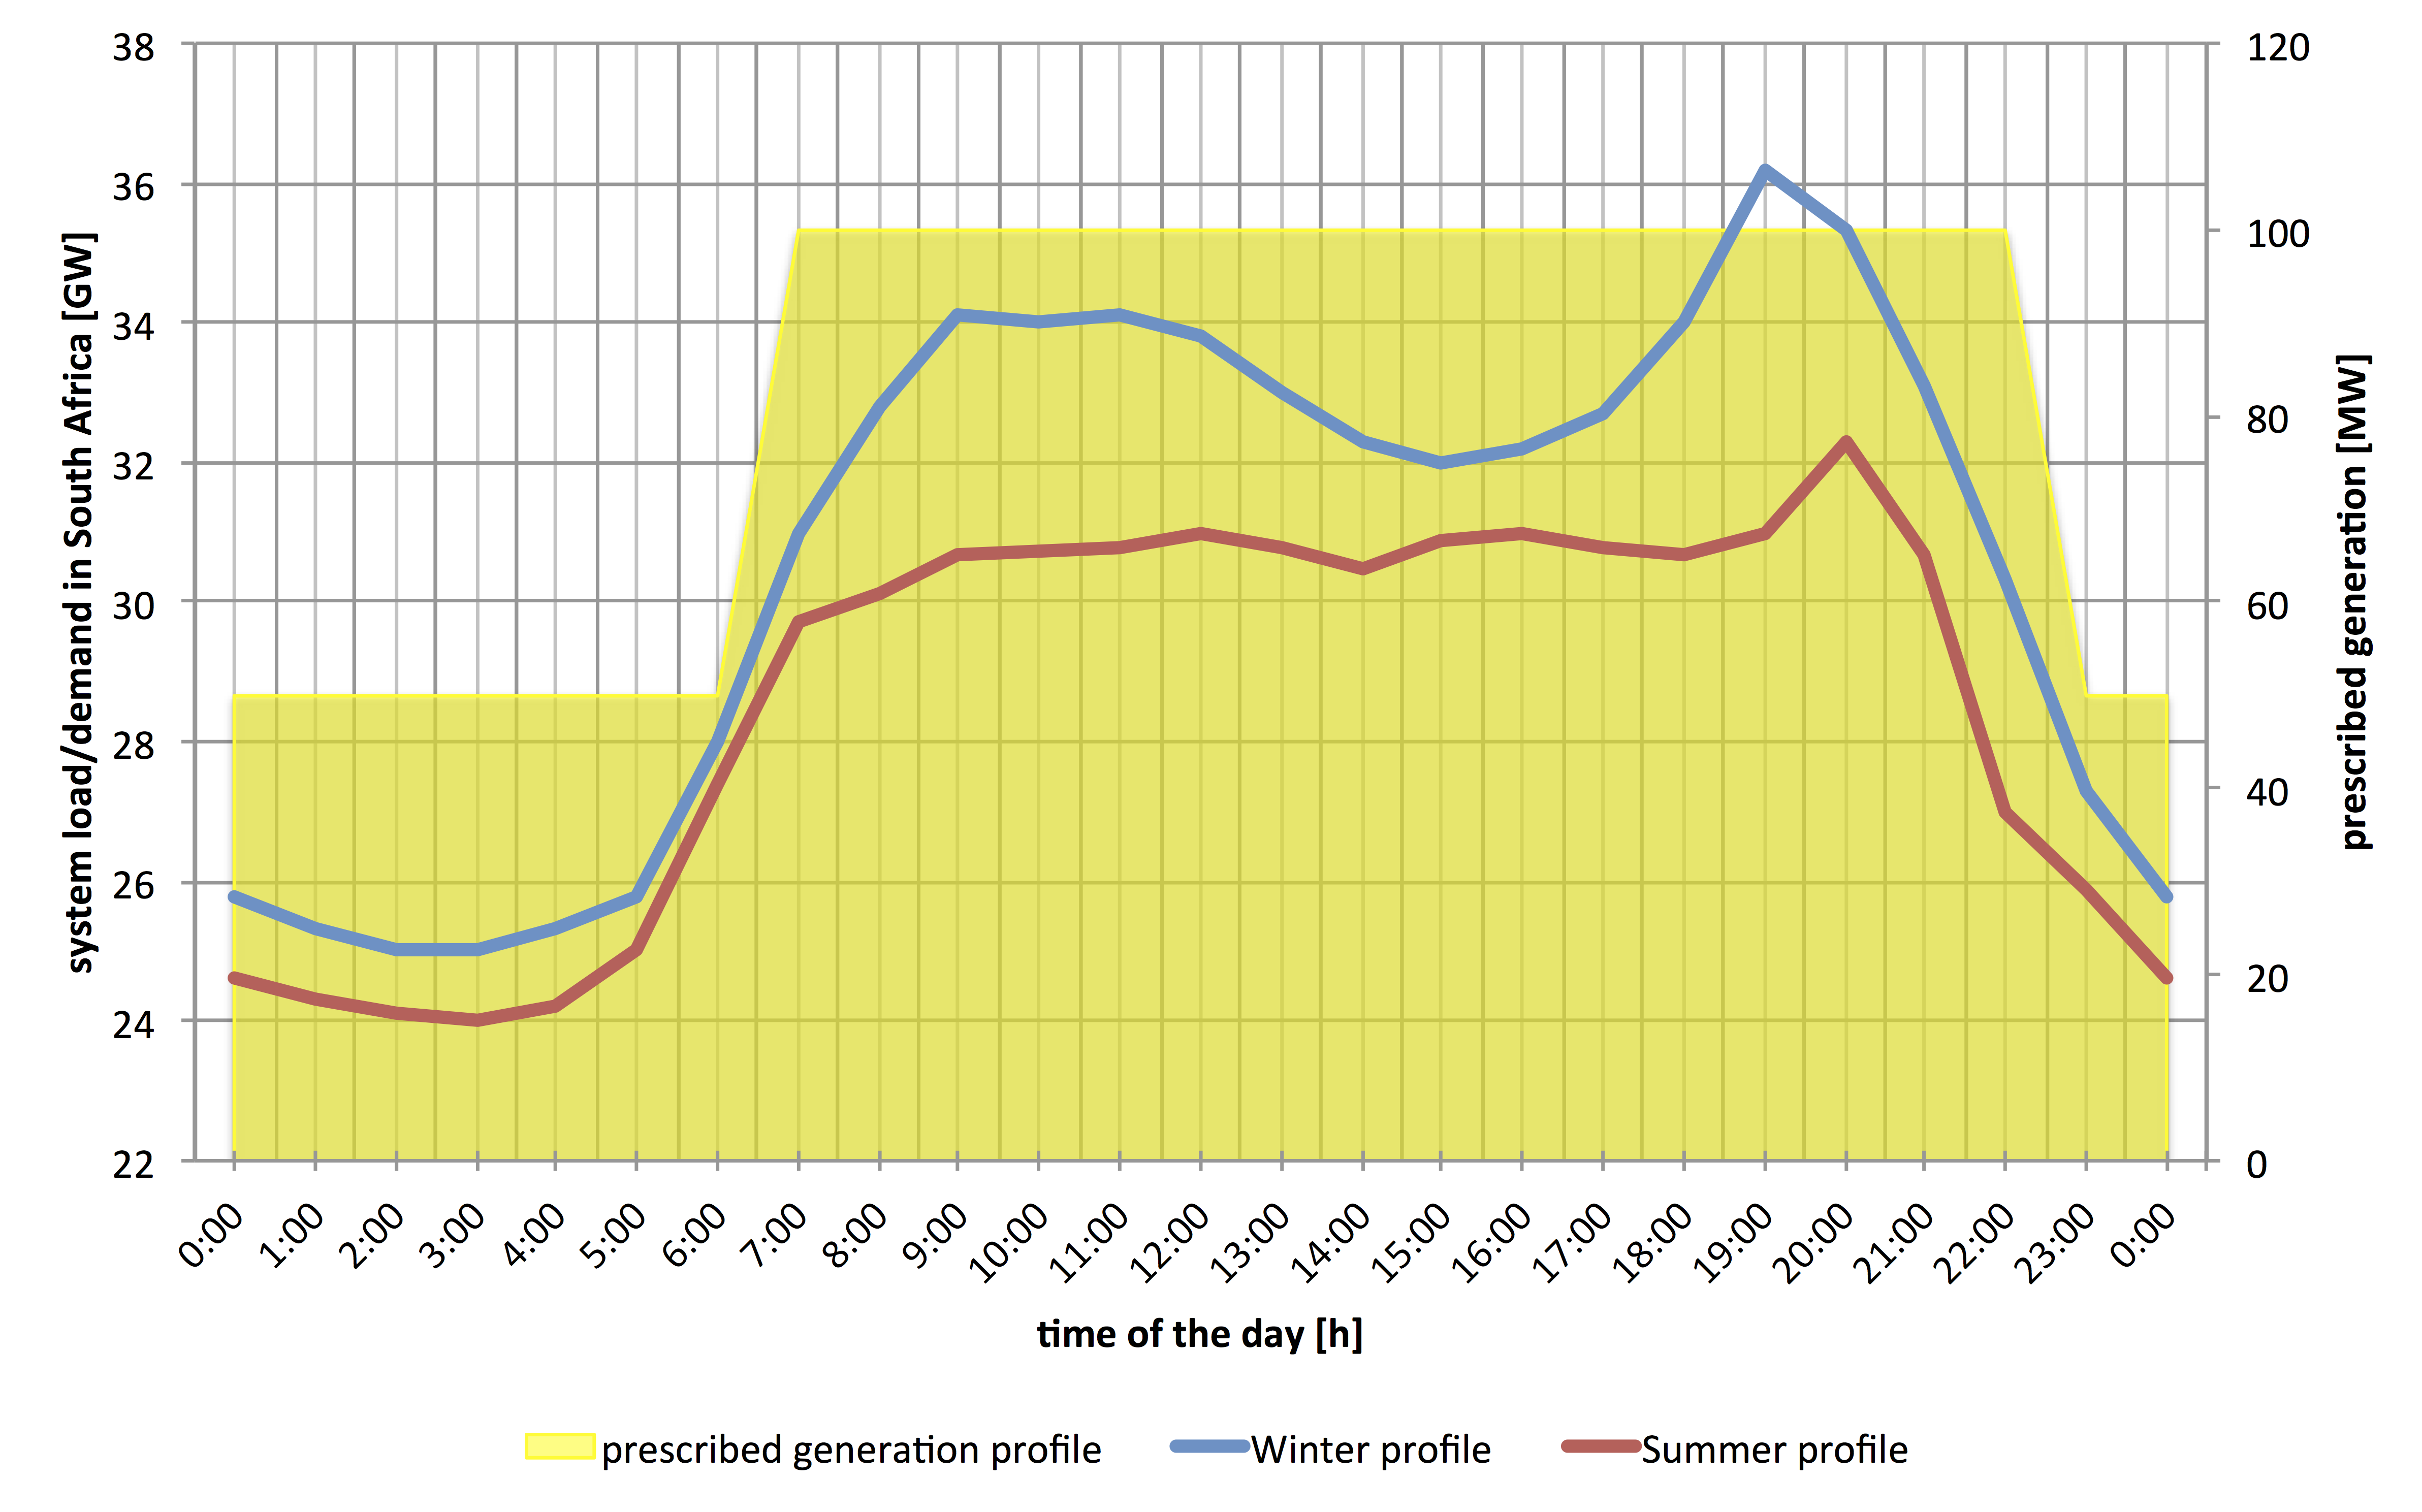
\includegraphics[width=1\linewidth]{FIG/LoadScenarios}
\caption[South Africa daily average system load/demand for summer and winter days, with scheduled power production curve.]{South Africa daily average system load/demand for summer and winter days, with scheduled power production curve.}\label{LoadScenarios}
\end{figure}
%For the comparison the power plants there system design is forced to cover 90~\% of the scheduled electricity production over the first year.  Usually, in feed-in contracts the power output is fixed at specified values. The overproduction is not content of these contracts and is not remunerated. In order to generate exploitable and comparable results and also considering the common feed-in contracts for power plants, the hourly power production is cut to the planed values. So overproduction will not considered in the evaluation and analyses of the systems.
In this comparison, the system design must handle 90~\% of the scheduled electricity production over the first year. Usually, in feed-in contracts, the deliverable energy is fixed. Any overproduction is not covered by such contracts and is not remunerated. In order to generate exploitable and comparable results and considering standard feed-in contracts, the hourly power production is cut to the planned values and thus overproduction is not considered in this analysis.

%The results of the simulated scenarios and the financial analyses will be rated in two selected categories:
The results of the simulation and the financial analyses will be evaluated by the following quantitative measures:
\begin{itemize}
%\item \textbf{Load curve covering factor} [\%]: The Load curve covering factor (LCCF) describes quantitative how effective the power plant follows the required load curve of the scenarios.
\item \textbf{Load curve covering factor} [\%]: The load curve covering factor (LCCF) is an effectiveness measure describing how closely the plant follows the load curve.
%\item \textbf{Levelized cost of electricity} [\textcent /kWh]: The levelized cost of electricity (LCOE) represents the total project lifecycle costs. It is the present value of project costs expressed in cents per kilowatt-hour of electricity generated by the system over its life. \cite{NREL2015a}
\item \textbf{Levelized cost of electricity} [\textcent /kWh]: The levelized cost of electricity (LCOE) represents the total project life-cycle costs. It is the present value of project costs expressed in cents per kilowatt-hour of electricity generated by the system over its life. \cite{NREL2015a}
\end{itemize}
%There is a huge difference between the mentioned LCCF and the widespread capacity factor (CF). The CF is the ratio of the system's predicted electrical output in the first year of operation to the nameplate output, which is equivalent to the quantity of energy the system would generate if it operated at its nameplate capacity for every hour of the year \cite{NREL2015a}. As it is mentioned above is the LCCF calculated from the sum value of load covering in each hour of the year.
There is an important difference between the LCCF and the widely-used \emph{capacity factor} (CF). The CF is the ratio of the system's electrical output in the first year of operation to the nameplate output, which is equivalent to the quantity of energy the system would generate if it operated at its nameplate capacity for every hour of the year \cite{NREL2015a}. The LCCF is calculated from the sum value of load coverage in each hour of the year. At a covering of 100~\% of the predicted load the solar power plants would produce \SI{711.75}{GWh} per year. But at a 100~\% CF the solar power plants would need to produce \SI{876.00}{GWh} per year. Therefore is in the selected scenario a maximum CF of just 81.25~\% with a full covering of the predicted load possible.

\subsection{Location and weather data} \label{Location and weather data}
%For the simulation of the solar power plants the locations and weather parameter of Upington, Northern Cape was used. This location is situated in a region with one of the highest irradiation values of the country, but also has a good water access by the Orange River. This locations was mentioned before in Chapter~\ref{Solar power in South Africa} and is marked in the GHI- and DNI-maps of SA in Figure \ref{irradiation} on Page \pageref{irradiation}.
In this simulation, locations and weather data for Upington, Northern Cape were used. This region has among the highest irradiation values in the country, but also has good water access due to the Orange River. This location was mentioned before in Chapter~\ref{Solar power in South Africa} and is marked in the GHI- and DNI-maps of SA in Figure \ref{irradiation} on Page \pageref{irradiation}. 
 
\begin{table}[!h]  
  \centering
	\begin{tabular}{  p{4.0cm}  C{4.0cm}  C{3.0cm} } 

	\hline	
\textbf{Item}  & \textbf{Value} & \textbf{Unit} \\ \hline \hline
Location & Upington & -\\ 
Station ID &  684240& -  \\ 
Data source & White Box Technologies, Inc. (31.05.2015) & -\\ \hline
Latitude & -28.40 &$\,^{\circ}$N \\ 
Longitude &  21.27 &$\,^{\circ}$E \\ 
Elevation &  836 & m \\ 
Total GHI per year  &  2~280 & \si{\kilo\watt\hour\per\square\metre}\\ 
Total DNI per year &  2~621 & \si{\kilo\watt\hour\per\square\metre}\\ 
Total DHI per year &  516 & \si{\kilo\watt\hour\per\square\metre}\\ 
Mean temp. &  21 & \si{\celsius}\\ 
Mean wind speed & 3.3 & \si{\metre\per\second}\\ \hline
\end{tabular}
\caption[Location and characteristics for the simulation in SAM.]{Location and characteristics for the simulation in SAM.}\label{tbl: Location}
\end{table}


%The input weather data for the simulation with SAM are in the EPW-format (EnergyPlus Weather Data) and produced by White Box Technologies, Inc. \cite{WhiteBoxTechnologies2015}. The EPW-files are data sets of hourly values of solar radiation and meteorological elements for a typical one-year period. This includes air temperature, dew point temperature, relative Humidity, atmospheric pressure, global horizontal solar radiation, diffuse Horizontal solar radiation, direct normal radiation, wind Speed, wind Direction and cloud cover. The for the simulation most relevant values are summarized in Table \ref{tbl: Location}. The hourly values of global horizontal and direct normal irradiance from the EPW-file is shown in Figure~\ref{Upington_GHI/DNI}. The highest irradiance value during the summer time is 1~\SI{199}{Wh/m}^2 for GHI and 1~\SI{154}{Wh/m}^2 for DNI. At the shortest day the highest irradiance is \SI{625}{Wh/m}^2 for GHI and \SI{820}{Wh/m}^2 for DNI.
The weather data for the simulation in SAM are in EPW format (EnergyPlus Weather Data) and produced by White Box Technologies, Inc. \cite{WhiteBoxTechnologies2015}. The EPW files are data sets of hourly values of solar radiation and meteorological elements for a typical one-year period. These include air temperature, dew point temperature, relative humidity, atmospheric pressure, global horizontal solar radiation, diffuse horizontal solar radiation, direct normal radiation, wind speed, wind direction and cloud cover. The most relevant parameters for this simulation are summarized in Table \ref{tbl: Location}. The hourly values of global horizontal and direct normal irradiance from the EPW file are shown in Figure~\ref{Upington_GHI/DNI}. The highest irradiance value during the summer is \SI{1199}{\watt\hour\per\square\metre} for GHI and \SI{1154}{\watt\hour\per\square\metre} for DNI. At the northern solstice, the highest irradiance is \SI{625}{\watt\hour\per\square\metre} for GHI and \SI{820}{\watt\hour\per\square\metre} for DNI.


\begin{figure}[!htbp]
        \centering
                \begin{subfigure}[b]{1\textwidth}
                \centering
                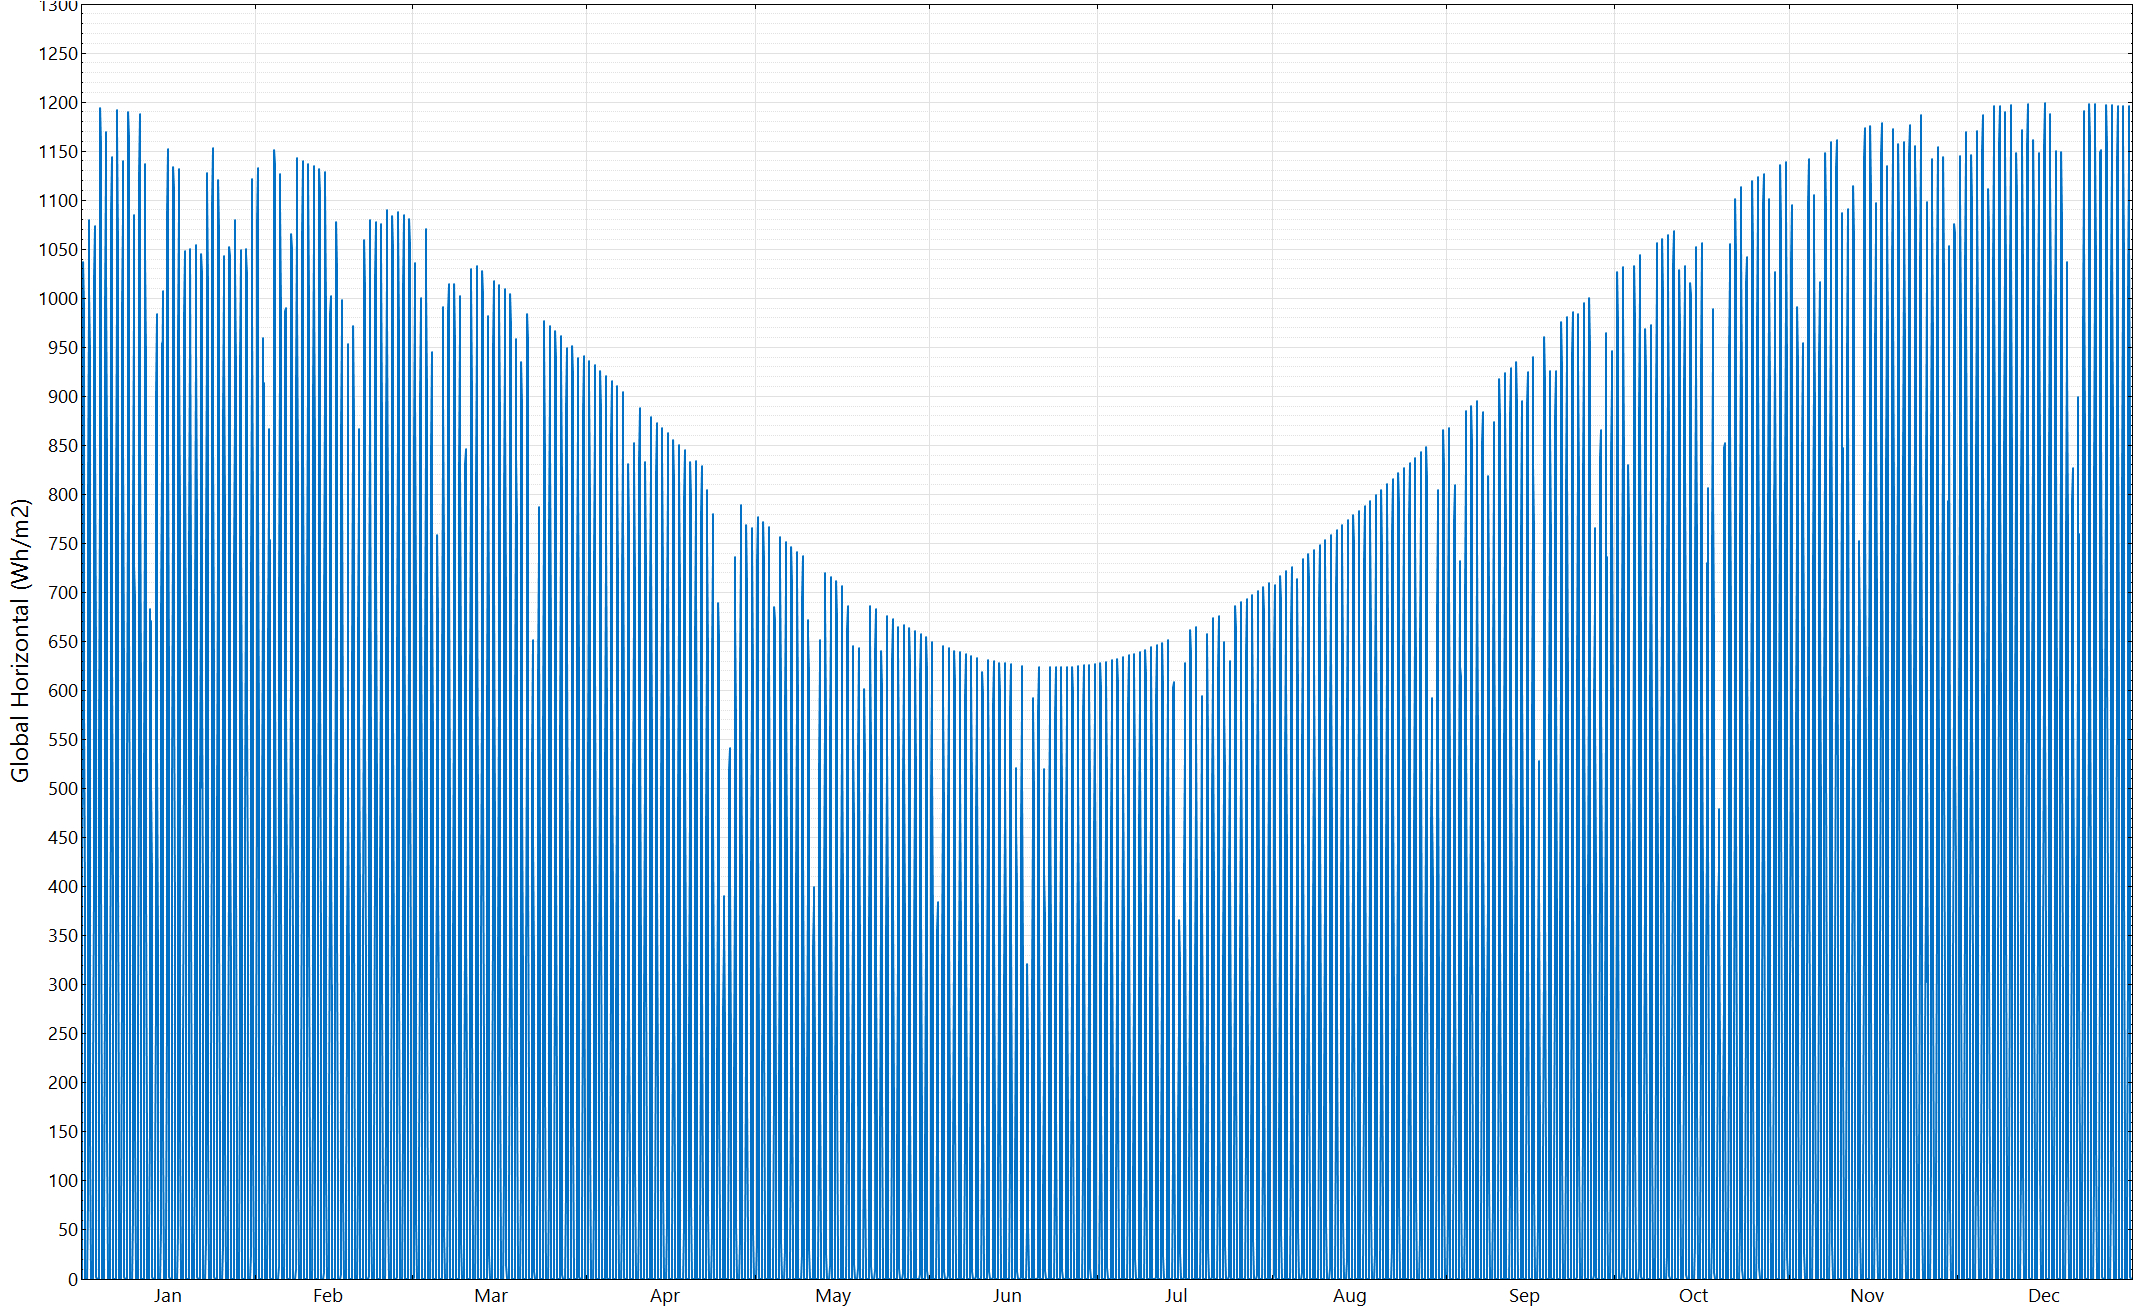
\includegraphics[width=1\textwidth]{FIG/Upington_GHI}
                \caption{Global horizontal}\label{Upington_GHI}
        \end{subfigure}%
\par\medskip % Linebreak      
        \begin{subfigure}[b]{1\textwidth}
                \centering
                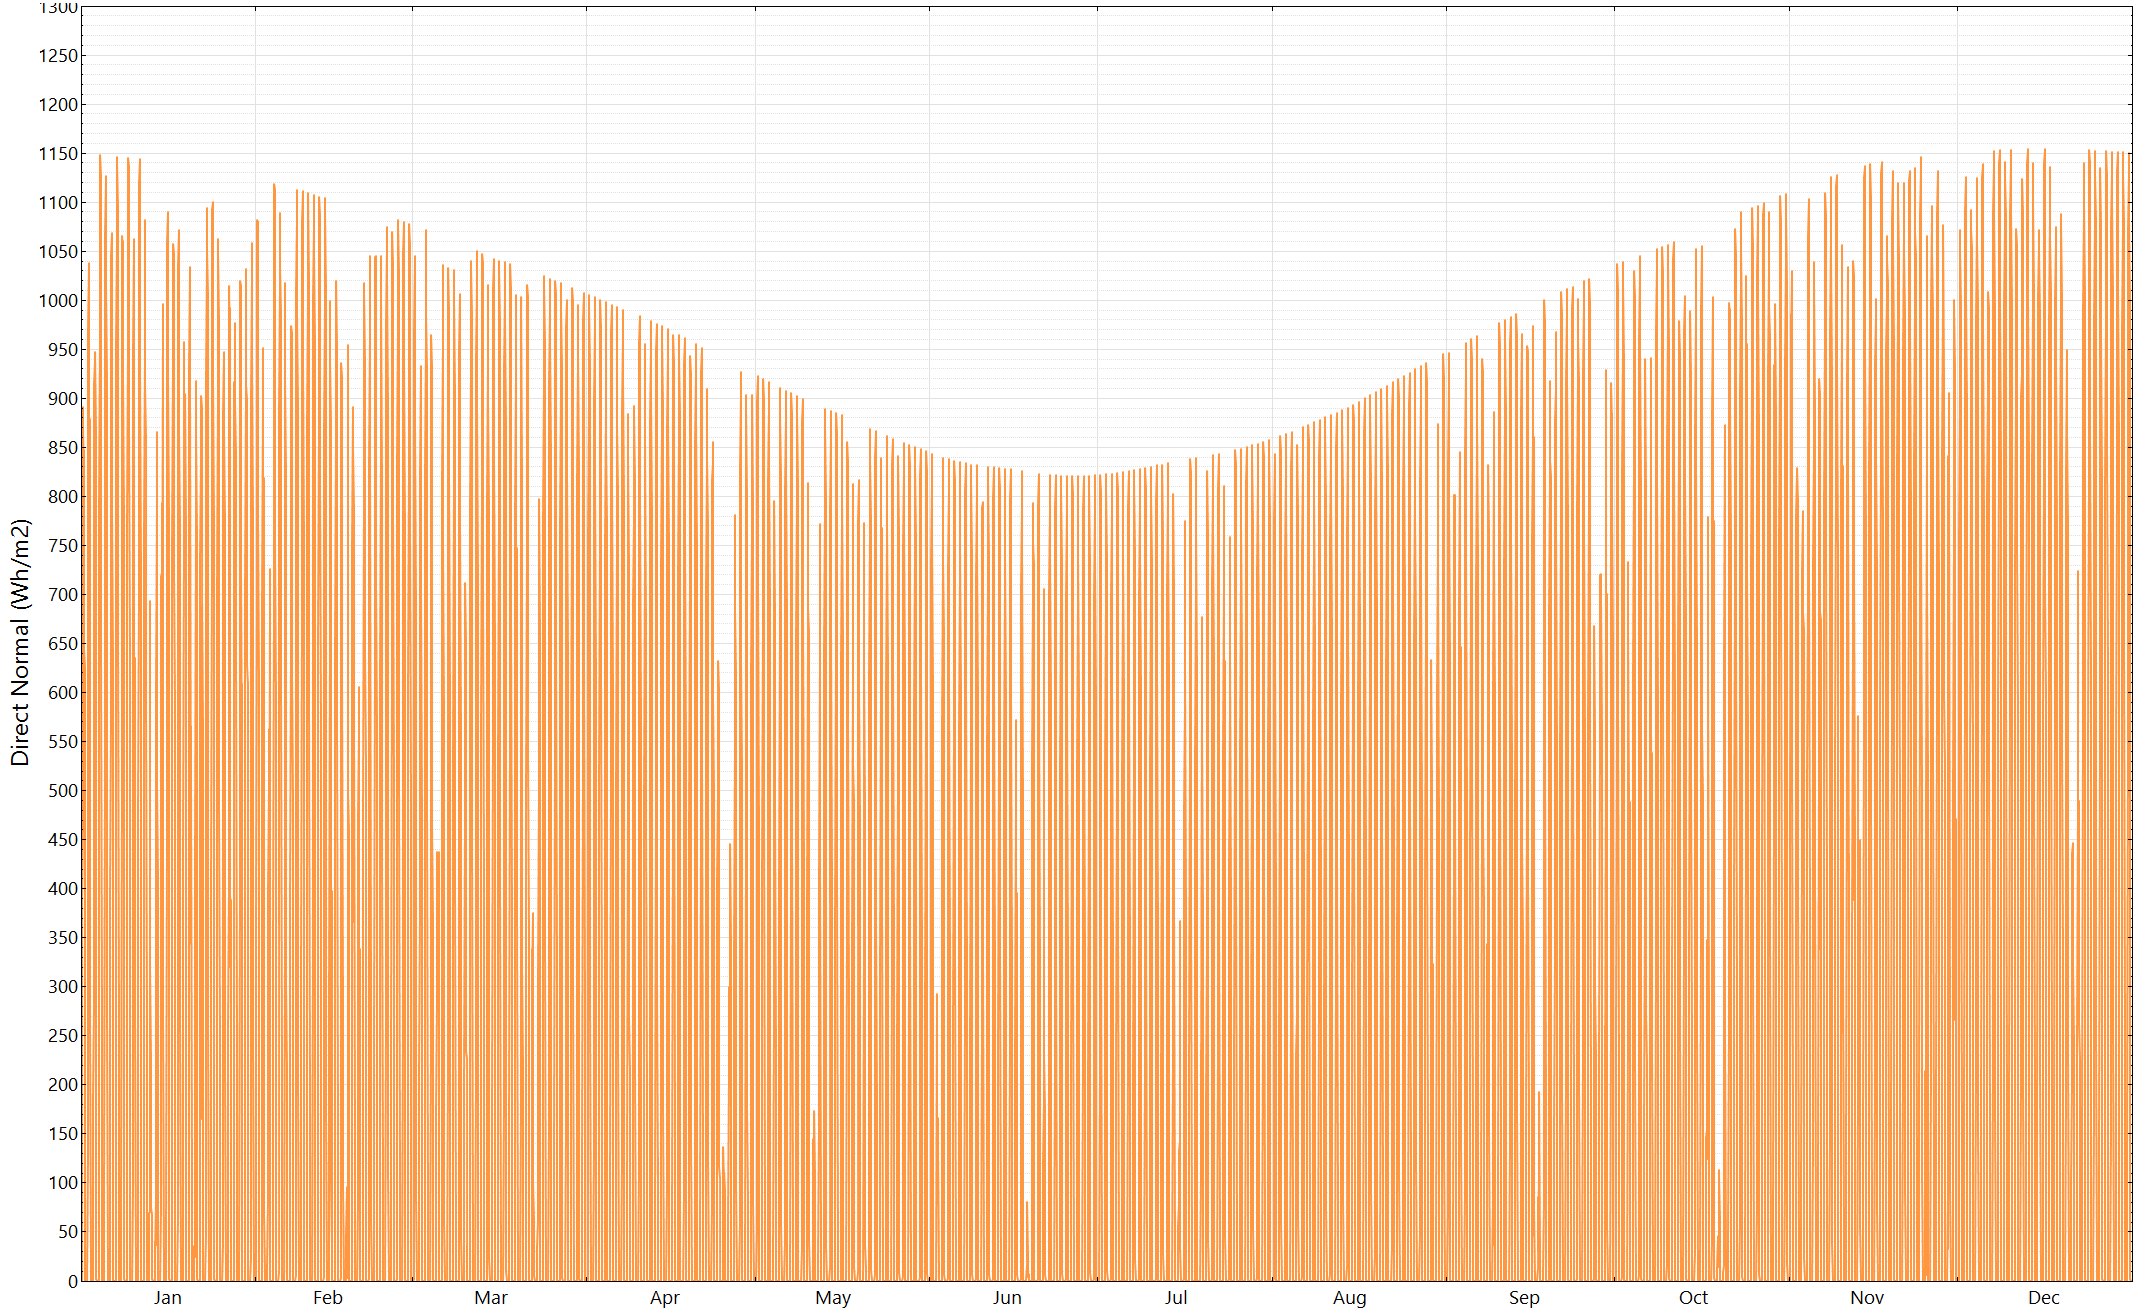
\includegraphics[width=1\textwidth]{FIG/Upington_DNI}
                \caption{Direct normal }\label{Upington_DNI}
        \end{subfigure}%

        \caption[Hourly values of irradiance over a full year from Upington used in the simulation.]{Hourly values of irradiance over a full year from Upington used in the simulation.}\label{Upington_GHI/DNI}
\end{figure}
\newpage \noindent
%Most relevant for the simulation is also the position of the sun. SAM calculates the path of the sun by the position of longitude and latitude. Figure~\ref{SunPathUpington} shows the sun path diagram of Upington. From this it appears that the longest day in Upington has \SI{13}{h} and \SI{56}{minutes} with a maximum sun height of 85.05$\,^{\circ}$ while the shortest day has just \SI{10}{h} and \SI{19}{minutes} and a maximum sun height of 35.93$\,^{\circ}$.
SAM calculates the path of the sun by the position of longitude and latitude. Figure~\ref{SunPathUpington} shows the solar path diagram at Upington. It is apparent that the longest day in Upington has a duration of \SI{13}{h} and \SI{56}{minutes} with a maximum sun height of \SI{85.05}{\degree} while the shortest day has a duration of just \SI{10}{h} and \SI{19}{minutes} and a maximum sun height of \SI{35.93}{\degree}.

\begin{figure}[htbp]  
\centering
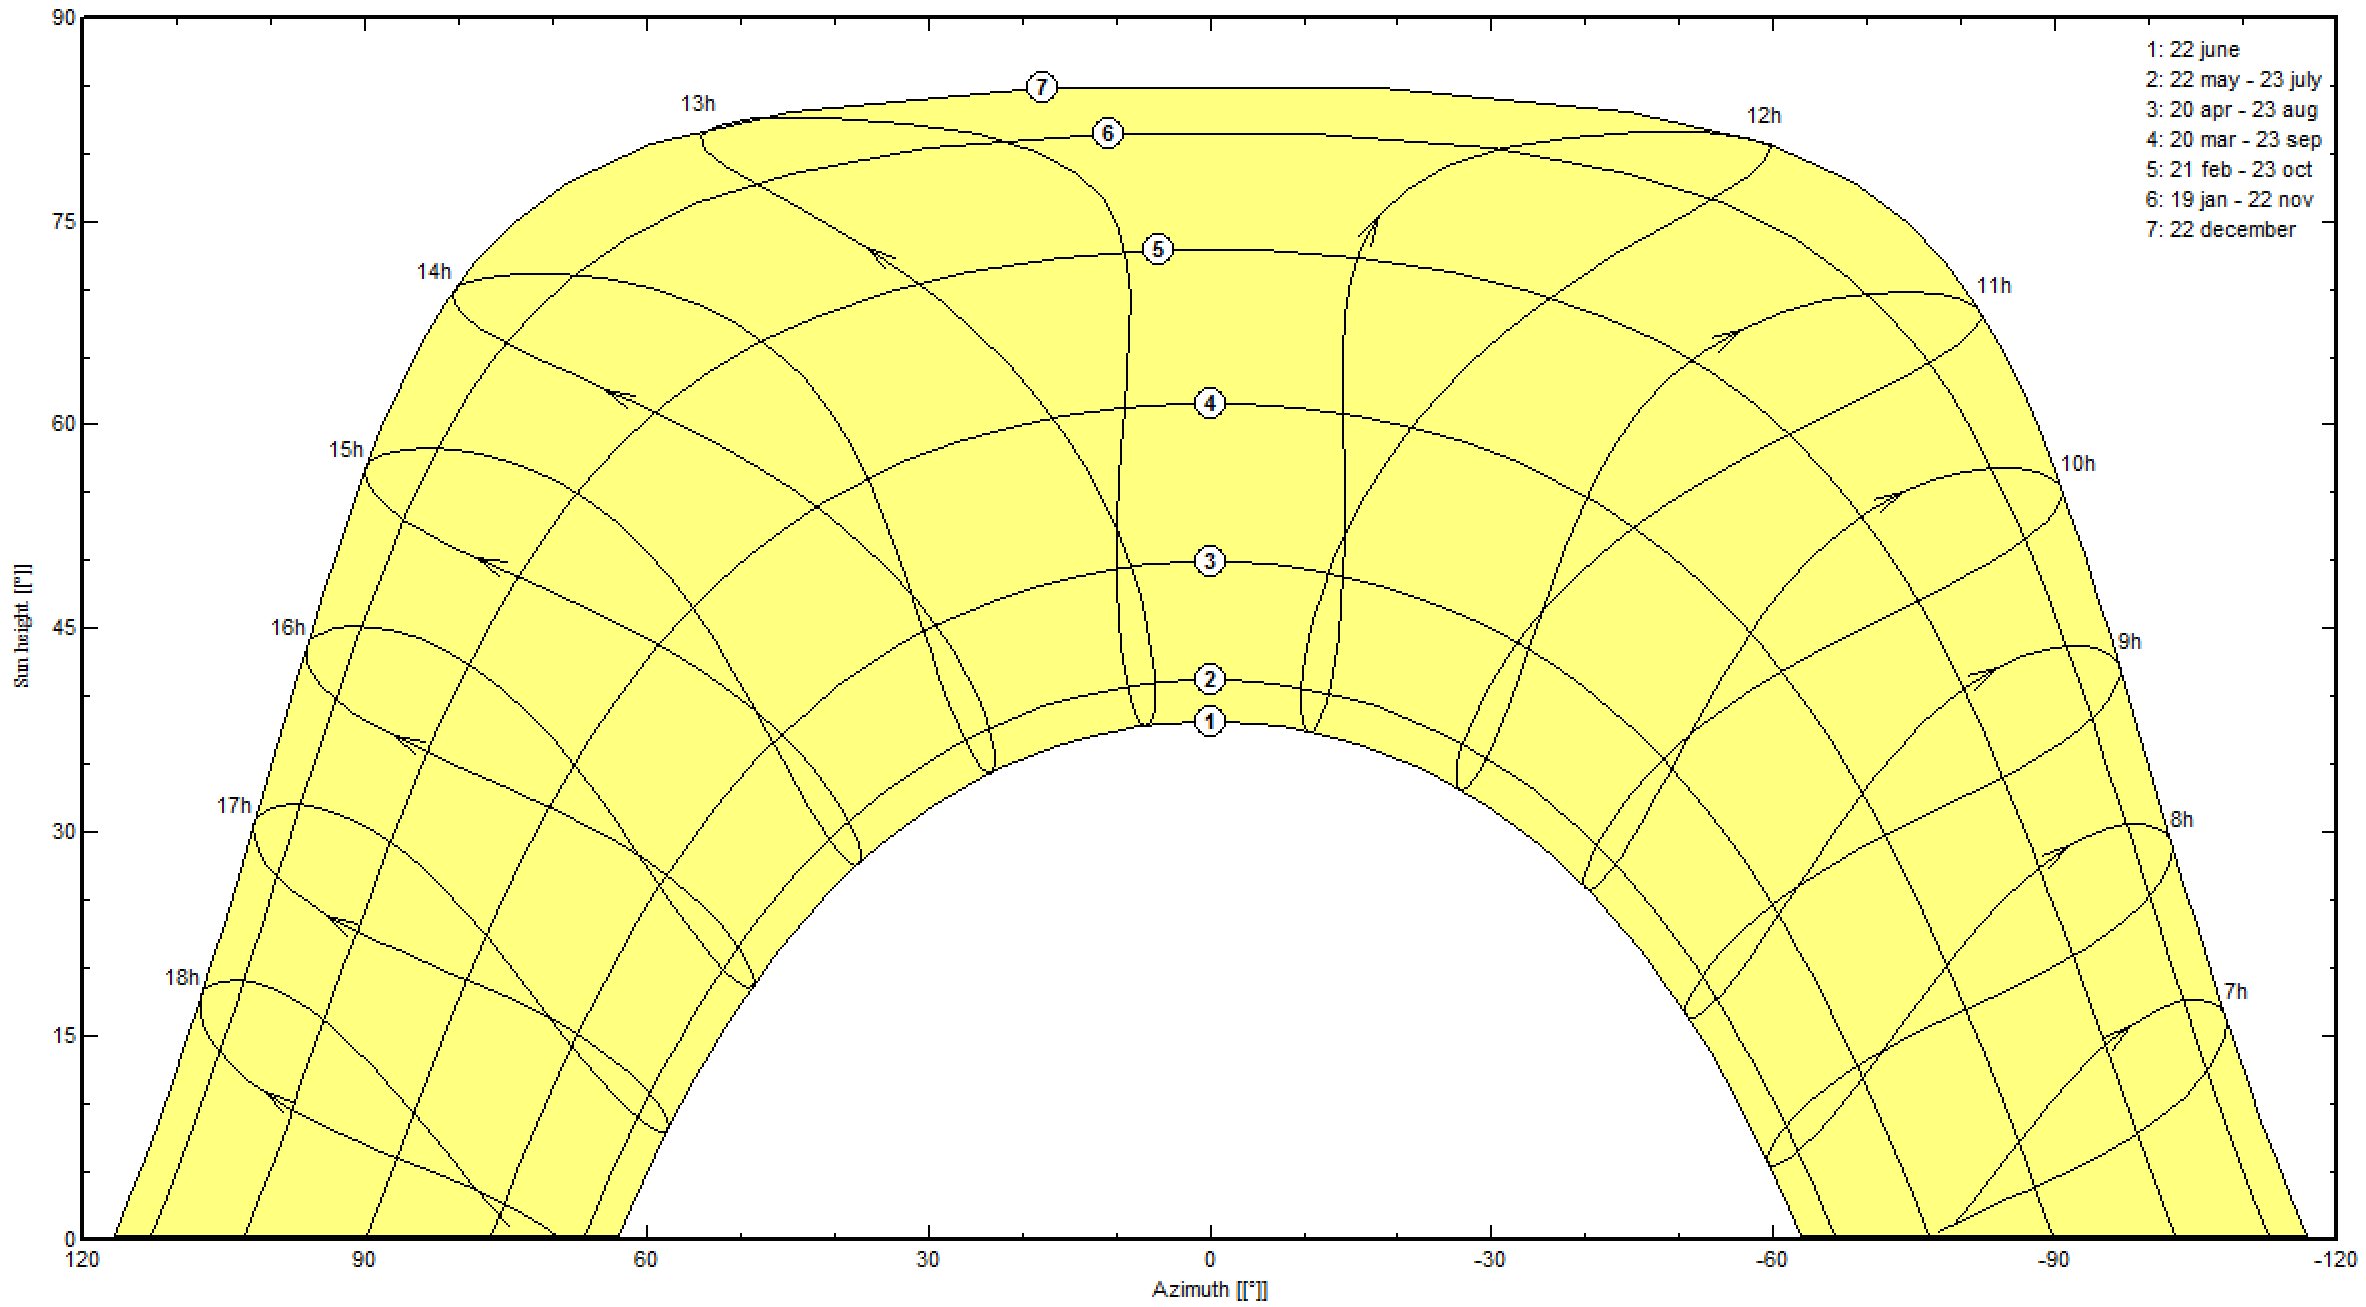
\includegraphics[width=0.95\linewidth]{FIG/SunPathUpington}
\caption[Solar path diagram for Upington.]{Solar path diagram Upington \cite{PVsystSA2015}.}\label{SunPathUpington}
\end{figure}
\pagebreak 
\section{CR power plant}
\subsection{Design  and simulation} \label{CR power plant design  and simulation}
%For the CR power plant simulation in SAM the “CSP power tower molten salt" model was used. The EPW weather file for Upington from Section~\ref{Location and weather data} was used as an input file to specify the hourly atmospheric conditions. SAM uses the following input data for the simulation:
For the CR plant simulation in SAM, the \enquote{CSP power tower molten salt} model was used. The EPW weather file for Upington from Section~\ref{Location and weather data} was used as an input file to specify the hourly atmospheric conditions. SAM uses the following input data for the simulation:
\begin{itemize}
\item Latitude (\si{\degree})
\item Longitude (\si{\degree})
\item Elevation above sea level (\si{\metre})
\item DNI (\si{\watt\per\square\metre})
\item Atmospheric pressure (\si{\milli\bar})
\item Dry bulb temperature (\si{\celsius})
\item Wet bulb temperature (\si{\celsius})
\item Relative humidity (\si{\percent})
\item Wind velocity (\si{\metre\per\second})
\end{itemize}
This Chapter describes in detail the crucial inputs of the CR power plant components, namely the power cycle, heliostat field, tower and receiver and thermal energy storage (TES).

As already mentioned, financial parameters and the LCOE are calculated separately in Microsoft Excel using a simplified method which is documented in Appendix~\ref{ChapterLCOE} on Page \pageref{ChapterLCOE}.

\subsubsection{Simulated configurations}
%The simulated configurations had the goal to reach 90~\% of the scheduled production curve by using variation of solar multiple and full load hours of TES. Also the simulated configurations covers a broad view on the technology possibilities. As already mentioned in Section~\ref{Large scale concentrated solar power (CSP) plants} is the SM the ratio of the receivers thermal output to the power cycles thermal input at design point. So a CR system with a SM of 1 has a receiver and a heliostat field which provides the thermal power needed for the power block to run at full load at the system design point. A receiver and collector field with a SM of 1 don't produce enough thermal power to store energy in a TES while feeding the turbine. A CR system with a SM of 1 is just suitable for systems without TES. To covering the scheduled load the solar multiple was varied from 2 to 3.5 in steps of 0.5. Also the storage full load hours were varied from 8 to \SI{16}{h} in steps of \SI{2}{h}. The target of \SI{100}{MW} net capacity was reached with a gross capacity of \SI{111}{MW} with an estimated gross-to-net conversion factor of 0.90. Table~\ref{tbl: CR_OverallConfig} summarizes the simulated configurations.
The simulated configurations were to meet 90~\% of the scheduled production curve by using variation of solar multiples and full load hours of TES. As mentioned in Section~\ref{Large scale concentrated solar power (CSP) plants} the solar multiple (SM) is the ratio of the receiver's thermal output to the power cycles thermal input at the design point. Thus, a CR system with a SM of 1 has a receiver and a heliostat field which provides the thermal power needed for the power block to run at full load at the system design point. A receiver and collector field with an SM of 1 do not produce enough thermal power to store energy in a TES while also feeding the turbine. A CR system with a SM of 1 is just sufficient for systems without TES. In order to cover the expected load, the solar multiple was varied from 2 to 3.5 in steps of 0.5, while storage full load hours were varied from 8 to \SI{16}{h} in steps of \SI{2}{h}. The target of \SI{100}{MW} net capacity was reached with a gross capacity of \SI{111}{MW} with an estimated gross-to-net conversion factor of \si{0.90}. Table~\ref{tbl: CR_OverallConfig} summarizes the simulated configurations.

\begin{table}[!h]  
  \centering
	\begin{tabular}{ p{4.0cm}  C{1.0cm} C{0.3cm} C{0.3cm} C{0.3cm} C{0.3cm} C{0.3cm} | C{0.3cm} C{0.3cm} C{0.3cm} C{0.3cm} C{0.3cm} } 
	\hline	
\textbf{Item} & \textbf{Unit} & \multicolumn{10}{c}{\textbf{Value}} \\ \hline \hline
Net turbine capacity & \si{\mega\wattel} & \multicolumn{10}{c}{100} \\
Gross turbine capacity & \si{\mega\wattel} & \multicolumn{10}{c}{111} \\ \hline
Solar multiple & - & \multicolumn{5}{c}{2.0} & \multicolumn{5}{c}{2.5} \\
TES capacity & h &  8 & 10 & 12 & 14 & 16 &  8 & 10 & 12 & 14 & 16 \\ \hline 
Solar multiple & - & \multicolumn{5}{c}{3.0} & \multicolumn{5}{c}{3.5} \\
TES capacity & h &   8 & 10 & 12 & 14 & 16 &  8 & 10 & 12 & 14 & 16 \\ \hline 
\end{tabular}
\caption[Simulated CR solar multiple and thermal energy storage configurations.]{Simulated CR solar multiple and thermal energy storage  configurations.}\label{tbl: CR_OverallConfig}
\end{table}
\subsubsection{Power cycle}
The power cycle of the simulated CR system features a Rankine-cycle steam engine, two open feed-water heaters, a pre-heater, boiler and super-heater \cite{NREL2015a}. As mentioned above has the turbine a gross capacity of \SI{111}{\mega\wattel} and a nameplate (net) capacity of 100 \si{\mega\wattel}. 
\begin{table}[!h]  
  \centering
	\begin{tabular}{  p{7.0cm}  C{2.0cm}  C{2.0cm} } 
	\hline	
\textbf{Item} & \textbf{Value} & \textbf{Unit} \\ \hline \hline
Turbine design capacity, gross  & 111 & \si{\mega\wattel} \\ 
Turbine design capacity, net & 100 & \si{\mega\wattel} \\ 
Boiler operating pressure & 125 & bar \\ 
Design inlet temperature & 288 & \si{\celsius} \\ 
Design outlet temperature & 566 & \si{\celsius} \\ 
Cycle conversion efficiency & 41.2 & \% \\ 
Steam generator design thermal power & 269.42 & \si{\mega\wattth}  \\
Power block start-up time & 0.5 & h \\ 
Minimum required start-up temperature & 500 & \si{\celsius} \\
Plant availability  & 96 & \\
Condenser type & air-cooled & - \\ 
\hline
\end{tabular}
\caption[CR power block and condecer input parameter in SAM.]{CR power block and condecer input parameter in SAM.}\label{tbl: CRPowerplant}
\end{table}
The steam generator has a HTF inlet temperature of \SI{566}{\celsius} and outlet temperature of \SI{288}{\celsius} at design point and operates at a pressure of \SI{125}{\bar}. In combination with a air-cooled condenser the CR power cycle system was simulated with a cycle gross efficiency of \SI{41.2}{\percent}. A wet-cooled condenser would reaches some higher efficiency, but because of the lack of water in the area of Upington and the requirement by the South African government for CSP plants, a air-cooled condenser was selected. The HTF inlet temperature, pressure and efficiency values where adapted for the configuration from \cite{Kolb2011a}. For starting up the system 
needs 30 minutes and a min. required temperature of \SI{500}{\celsius}. A plant availability of 96~\% was adapted from \cite{Morin2012} in order to simulate system down-times for outages or scheduled maintenance.
\subsubsection{Heliostat field}
The heliostat field design was done in SAM using its heliostat field layout optimization tool. For the design, optimization and simulation process, heliostat data from the Sanlúcar 120 heliostat was used \cite{Noone2012}. The Sanlúcar 120 is used in the Planta Solar 10 (PS10) near Seville, Spain and is the origin of Abengoas actual heliostat ASUP 140. For a simulation with the ASUP 140 no sufficient data was available. 
\begin{table}[!htbp]  
  \centering
	\begin{tabular}{ p{4.5cm}  C{1.5cm} C{1.2cm} C{1.2cm} C{1.2cm} C{1.2cm} } 
	\hline	
\textbf{Item} & \textbf{Unit} & \multicolumn{4}{c}{\textbf{Value}} \\ \hline \hline
racking & - &  \multicolumn{4}{c}{two-axis} \\
Height & m  &  \multicolumn{4}{c}{9.45} \\
Width & m  &  \multicolumn{4}{c}{12.84} \\
Reflective area & \si{\square\metre} &  \multicolumn{4}{c}{120.00} \\
Heliostat availability& \% &  \multicolumn{4}{c}{99} \\
Design-point DNI & \si{\watt\per\square\metre} &  \multicolumn{4}{c}{950} \\
\hline
\textbf{Solar multiple}& \textbf{-} & \textbf{2.0} & \textbf{2.5} & \textbf{3.0} & \textbf{3.5}\\ \hline 
Number of heliostats & - & 9~131 & 11~530 & 13~976 & 16~658 \\
Max. distance from tower & m & 1~528 & 1~708 & 1~883 & 2010 \\
Reflective area  & ha & 109.58 & 138.36 & 167.72 & 199.90 \\
Field land area & ha & 655.59 & 821.92 & 997.95 & 1~190.99 \\ 
\hline
\end{tabular}
\caption[CR heliostat parameter.]{CR heliostat parameter.}\label{tbl: CRHeliostats}
\end{table}
The Sanlúcar 120 heliostats have an effective reflective area of \SI{120}{\square\metre} and are tracked on 2 axes. The heliostat field layout optimization and there design depends on the turbine gross and the SM. The heliostat field was optimized therefore for all four considered configurations. SAM first generates a coarse layout and optimizes the number of heliostats and their position. The goal of the optimization is the maximum flux with minimum power constraints according to the specified design-point DNI which represents the DNI at which the power plant achieves its rated thermal capacity. Table~\ref{tbl: CRHeliostats} summarizes the heliostat datas and the values of the optimized field design for all considered solar multiples.

The optimized heliostat field layouts of the four considered SM are depict in Figure~\ref{SM}. In order to avoid mutual shading from the heliostats the heliostat density decreases with distance from the tower. The maximum heliostat distance to the tower rises with the higher SM which can be seen in the field diameter. 
\begin{figure}[!htbp]
        \centering   
        \begin{subfigure}[b]{0.5\textwidth}
                \centering
                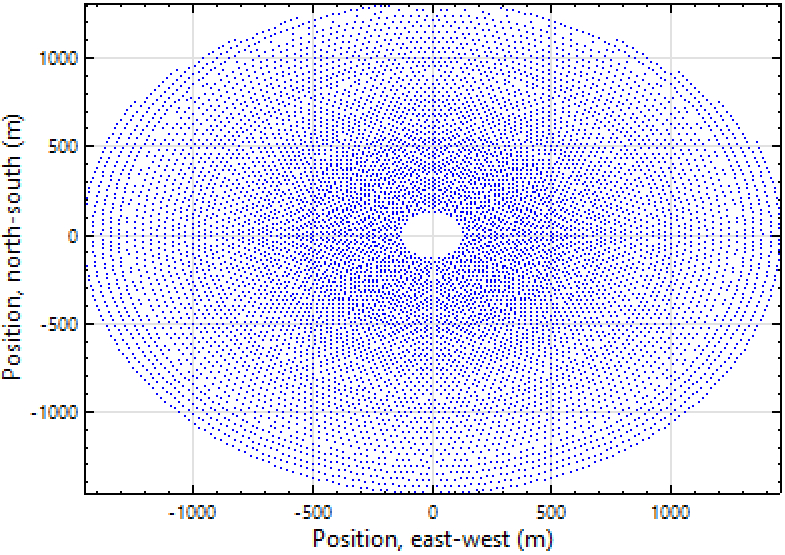
\includegraphics[width=0.95\textwidth]{FIG/SM20}
                \caption{SM:~2.0}\label{SM2.0}
        \end{subfigure}%
        ~
        \begin{subfigure}[b]{0.5\textwidth}
                \centering
                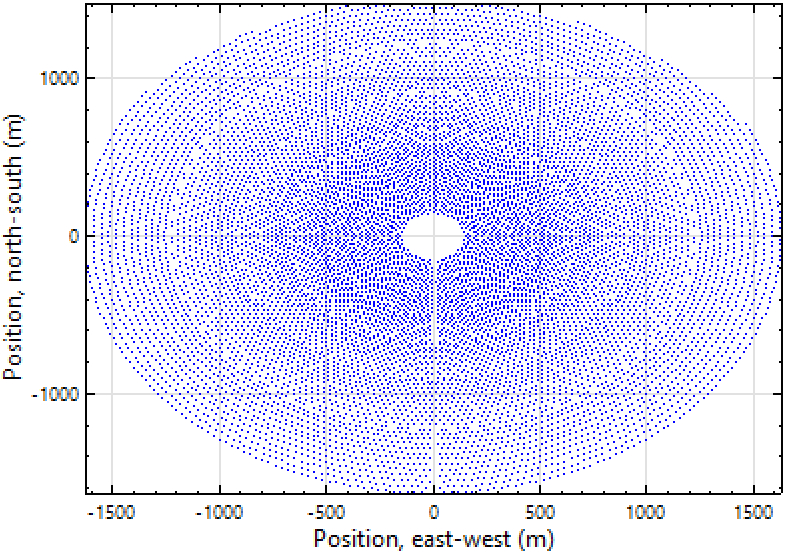
\includegraphics[width=0.95\textwidth]{FIG/SM25}
                \caption{SM:~2.5}\label{SM2.5}
        \end{subfigure}
        
\par\medskip % Linebreak
                
        \begin{subfigure}[b]{0.5\textwidth}
                \centering
                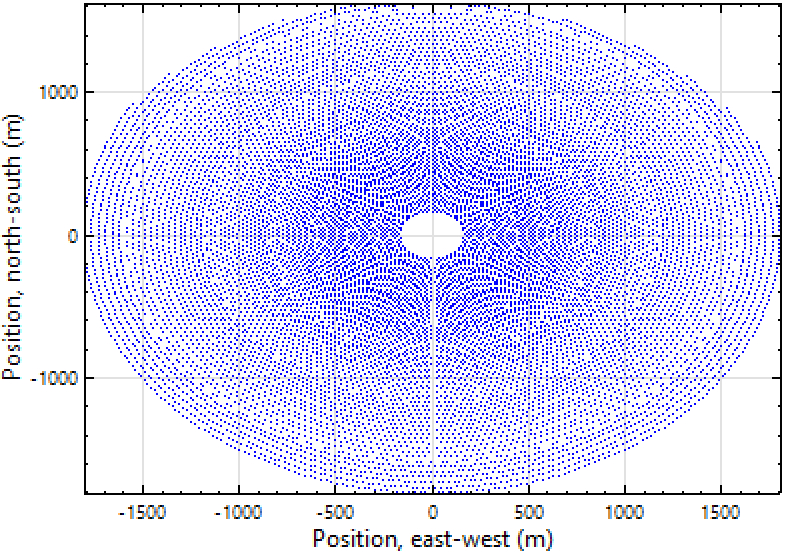
\includegraphics[width=0.95\textwidth]{FIG/SM30}
                \caption{SM:~3.0}\label{SM3.0}
        \end{subfigure}%
        ~
        \begin{subfigure}[b]{0.5\textwidth}
                \centering
                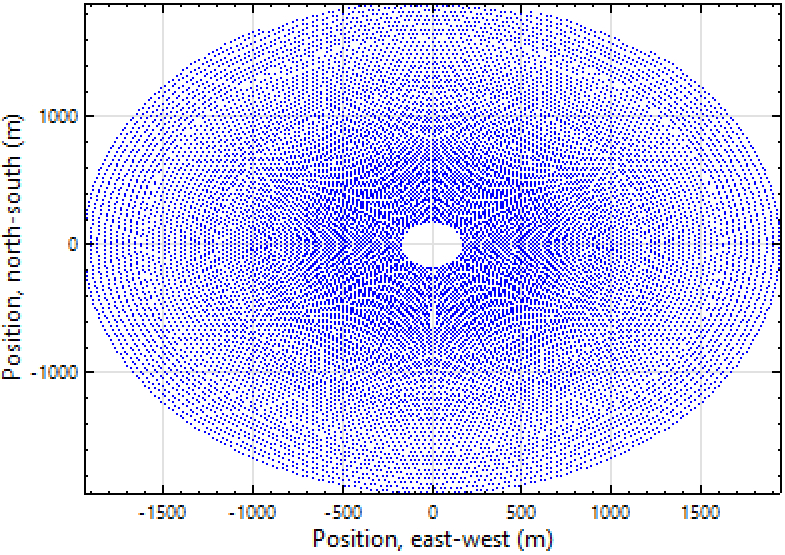
\includegraphics[width=0.95\textwidth]{FIG/SM35}
                \caption{SM:~3.5}\label{SM3.5}
        \end{subfigure}
        \caption[Simulated heliostat field layout at diferent solar multiples (SM).]{Simulated heliostat field layout at diferent solar multiples (SM).}\label{SM}
\end{figure}
\subsubsection{Tower and receiver}
The receiver collects the concentrated irradiance from the surrounding heliostat field. The simulated receiver is build as an external cylindrical receiver and is configurated with 24 panels of thin walled (1.25 mm) receiver tubes with an outer diameter of 60 mm arranged in a circle around the tower. The receiver tubes are made from 316H stainless steel and the external surfaces of the tubes are coated with a black Pyromark paint. The paint is resistant to high temperatures and thermal cycling, and absorbed 95\% of the incident sunlight. This configuration is similar to the receiver of the  Solar Two Project accept of the outer diameter \cite{Bradshaw2002}. The panels containing molten salt (60~\% NaNO\textsubscript{3} and 40~\% KNO\textsubscript{3}) as heat transfer fluid (HTF). The receiver design inlet temperature of 288$\,^{\circ}\mathrm{C}$ and the outlet temperature of 566$\,^{\circ}\mathrm{C}$ was set before in the power block configuration. In order to achieve the desired receiver thermal power output, the height of the tower and receiver dimensions got also adjust with the optimization of the heliostat field design. The results of the optimization is shown in Table~\ref{tbl: CRSolarfield}, as well as the fixed tower and receiver parameter. The heights of the tower range from 179.77 to \SI{236.50}{m}. The receiver proportions rises with the SM and the field sizes and results in a receiver thermal power range from 538.8 to 943.0 \si{\mega\wattth}.
\begin{table}[!h]  
  \centering
	\begin{tabular}{ p{5.5cm}  C{1.5cm} C{1.2cm} C{1.4cm} C{1.4cm} C{1.4cm} } 
	\hline	
\textbf{Item} & \textbf{Unit} & \multicolumn{4}{c}{\textbf{Value}} \\ \hline \hline
Receiver configuration & - &  \multicolumn{4}{c}{external cylindrical receiver}\\
Heat transfer fluid & - &  \multicolumn{4}{c}{60~\% NaNO\textsubscript{3} and 40~\% KNO\textsubscript{3}}\\
Inlet temperatures & $\,^{\circ}\mathrm{C}$  &  \multicolumn{4}{c}{288}\\
Outlet temperatures & $\,^{\circ}\mathrm{C}$  &  \multicolumn{4}{c}{566}\\
Receiver tube material & - &  \multicolumn{4}{c}{AISI316 stainless steal}\\
Receiver tube outer diameter & \si{\milli\metre} &  \multicolumn{4}{c}{60}\\
Receiver tube wall thickness & \si{\milli\metre} &  \multicolumn{4}{c}{1.25}\\
Number of panels & - &  \multicolumn{4}{c}{24}\\
Absorption factor  & - &  \multicolumn{4}{c}{0.95}\\
\hline
\textbf{Solar multiple} &  & \textbf{2.0} & \textbf{2.5} & \textbf{3.0} & \textbf{3.5}\\ \hline 
Tower height & \si{\metre} & 179.77 & 200.96 & 221.57 &  236.50\\
Receiver height  & \si{\metre} & 22.55 & 25.45 & 27.74 &  29.94\\
Receiver diameter & \si{\metre} & 14.85 & 16.66 & 17.91 & 18.77\\ 
Receiver aperture area & \si{\square\metre} & 1~052 & 1~332 & 1~561 & 1~765 \\ 
Receiver thermal power & \si{\mega\wattth} & 538.8 & 673.5 & 808.3 & 943.0 \\
\hline
\end{tabular}
\caption[CR heliostat field parameter.]{CR heliostat field parameter.}\label{tbl: CRSolarfield}
\end{table}
\subsubsection{Thermal energy storage (TES)}
The CR system was simulated using a direct two-tank molten salt thermal energy storage (TES). The storage uses directly the HTF (60~\% NaNO\textsubscript{3} and 40~\% KNO\textsubscript{3}) from the receiver as storage medium. Figure~\ref{towerdirecttwotank} on Page~\pageref{towerdirecttwotank} shows a schema of the direct storage for CR system. The design temperature of the hot storage tank (566$\,^{\circ}\mathrm{C}$) and the cold storage tank (288$\,^{\circ}\mathrm{C}$) depends also from the set value in the power block settings as before the design receiver temperatures. So the design temperature difference between the tanks is 278$\,^{\circ}\mathrm{C}$.



As defined at the beginning of this Chapter, the full load hours of TES are varied in steps of \SI{2}{h} from 8 to \SI{16}{h}. The TES full load hours represents the time in which the storage can supply enough energy to the steam turbine and the power block to run at full design capacity. So a higher value of TES full load hours extended the time that the power plant can run during nights or cloudy days. Table~\ref{tbl: CRTES} shows that with higher TES full load hours the thermal capacity and tank volume increases as well. The simulated storage capacity is in a range of 2~\SI{155}{\mega\wattth\hour} using 8 full load hours and 4~\SI{311}{\mega\wattth\hour} using 16 full load hours. 
\begin{table}[!h]  
  \centering
	\begin{tabular}{ p{3.9cm}  C{1.0cm} C{1.2cm} C{1.2cm} C{1.2cm} C{1.2cm} C{1.2cm} } 
	\hline	
\textbf{Item} & \textbf{Unit} & \multicolumn{5}{c}{\textbf{Value}} \\ \hline \hline
Storage type & - &  \multicolumn{5}{c}{direct two-tank molten salt}\\
Storage fluid & - &  \multicolumn{5}{c}{60~\% NaNO\textsubscript{3} and 40~\% KNO\textsubscript{3}}\\
Hot tank design temp. & \si{\celsius} & \multicolumn{5}{c}{566}\\
Cold tank design temp. & \si{\celsius} & \multicolumn{5}{c}{288}\\
\hline
\textbf{TES full load hours} & \textbf{h} & \textbf{8} & \textbf{10} & \textbf{12} & \textbf{14} & \textbf{16}\\ \hline 
Thermal capacity & \si{\mega\wattth\hour} & 2~155 & 2~694 & 3~233 & 3~772 &  4~311\\
Storage volume  & \si{\cubed\metre} & 10~229 & 12~787 & 15~345 & 17~902 & 20~460\\
\hline
\end{tabular}
\caption[CR system TES parameter.]{CR system TES parameter.}\label{tbl: CRTES}
\end{table}

SAM 2015.6.30 r3 don't have a power control to follow prescribed hourly net output values. The turbine output of each day needs to be scheduled in front for the simulation. Thereby the parasitic consumer needs highly attention. Figure~\ref{CR_turbineoutput} shows the for the simulation scheduled turbine output matrix. The individual values was fixed during experimental trial. It can be seen that the turbine output is reduced to 50\% during the night as it is specified in the scenario. The power plant follows the schedule till there is no solar irradiance and no more thermal capacity in the storage left to generate power. 
\begin{figure}[htbp]  
\centering
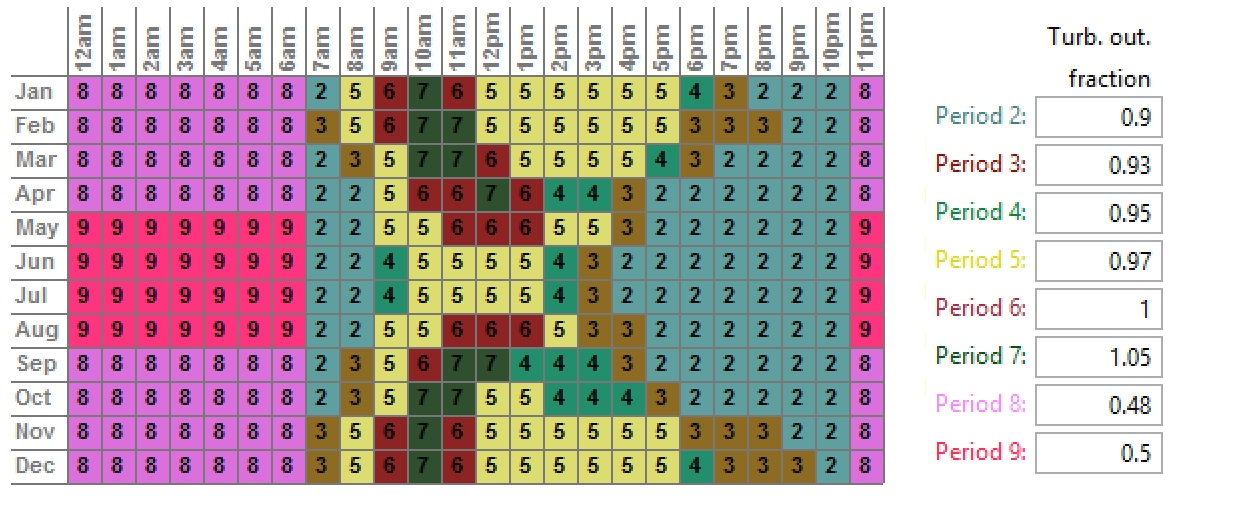
\includegraphics[width=0.95\linewidth]{FIG/CR_turbineoutput}
\caption[TES dispatch control matrix for turbine output fraction of CR simulation in SAM.]{TES dispatch control matrix for turbine output fraction of CR simulation in SAM.}\label{CR_turbineoutput}
\end{figure}
\pagebreak
\subsubsection{Financial parameter}
The financial parameter for the LCOE calculation of the CR power plant are seperated in different specific cost parts and are sumerized in Table~\ref{tbl: CRFinance}. The method for calculating the LCOE is documented in Appendix~\ref{ChapterLCOE} on Page \pageref{ChapterLCOE} using a lifetime of \SI{25}{years} and a real interest rate of 7.5~\% \cite{FraunhoferISE2013}. The interest rate could be reduced with a rising market potential.



The specific costs of the heliostat field of \SI{180}{\usd\per\square\metre} coming from J. B. Blackmon \cite{Blackmon2012}. He analyzed the costs of heliostat as a function of area for a representative solar central receiver power plant and calculated the total installed costs for a field of 5~000 heliostats with \SI{148}{\square\metre} reflective area of approximately \SI{180}{\usd\per\square\metre}. The analyze results showed that the costs are increasing with the size of the heliostats from \SI{40}{\square\metre} on. So the adopted value of \SI{180}{\usd\per\square\metre} reflective area for \SI{140}{\square\metre} heliostats can be assumed as conservative.

The remaining investment costs are based on the "Power Tower Technology Roadmap and Cost Reduction Plan" \cite{Kolb2011} from 2011.

On top of the investment costs a came 15 \% once-off surcharge for EPC and contingencies \cite{Platzer2014}.

Fichtner analyzed the annual O\&M costs with 1.84-1.96~\% of the total investment costs for CR power plants in SA \cite{Fichtner2010}. The value of 2~\% can so also be assumed as conservative.

The costs for the land purchase comes from the "African Agriculture Review" report of the Nedbank Capital, which reported the prices for farmland in SA. For the LCOE calculation of the CSP and PV system was the land purchase costs of 3~\SI{000}{USD/ha} assumed which is based on these report \cite{Cassell2012}.

\begin{table}[!h]  
  \centering
	\begin{tabular}{  p{5.0cm} C{2.0cm} C{1.5cm}  C{1.5cm}  C{4.0cm} } 
	\hline	
\textbf{Item} & \textbf{Symbol}& \textbf{Value} & \textbf{Unit} & \textbf{Source}\\ \hline \hline
Heliostat field &$c_{HF}$ & 180 & \si{\usd\square\metre} & \cite{Blackmon2012}\\ 
Power block & $c_{PB,CR}$ & 1000 & \si{\usd\per\kilo\wattel} & \cite{Kolb2011}\\ 
Thermal energy storage&$c_{TES,CR}$ & 30 & \si{\usd\per\kilo\wattth\hour}  & \cite{Kolb2011}\\ 
Tower and receiver& $c_{T+R}$& 200 & \si{\usd\per\kilo\wattth} & \cite{Kolb2011}\\ 
Annual O\&M & $f_{O\&M,CR}$ & 2 & \% &\cite{Fichtner2010}\\
Land purchase&$c_{LP}$ & 3~000 & \si{\usd\per\hectare} & \cite{Cassell2012}\\ \hline
Lifetime &$n$ & 25 & \si{\year} & \cite{FraunhoferISE2013} \\ 
Interest rate & $i_{CR}$ & 7.5 & \si{\percent} & \cite{FraunhoferISE2013} \\ 
Annual insurance costs& $f_{ins,CR}$ & 0.5 & \si{\percent} & \cite{IRENA2012}\\
Surcharge for EPC, project management and risk & $f_{EPC,CR}$& 15 & \si{\percent} & \cite{Platzer2014} \\
Total plant availability & $f_{avail,plant,CR}$ & 96 & \si{\percent} & \cite{Morin2012} \\ 
\hline
\end{tabular}
\caption[Finacial input parameter for CR-simulation in SAM.]{Finacial input parameter for CR-simulation in SAM.}\label{tbl: CRFinance}
\end{table}
\subsection{Results of CR power plant simulation}
The following sections illustrates and discuss the obtained simulation and calculation results of the above defined CR power plant. Therefore the load curve covering performance and LCOE as well as the belonging load profiles and duration curves are described and analyzed. The configuration of the power plants to reach 90~\% of the prescribed load while using the best belonging LCOE is defined at the end of each section.
\subsubsection{Load curve covering}
To find the suitable power plant configuration of the CR system to reach the target of 90~\% load curve covering, there was 20 various configurations simulated. This section presets and compare mainly the results of the simulation with the lowest SM and hours of TES configuration (SM: 2.0 \& TES: \SI{8}{h}) with the simulation using the highest SM and hours of TES configuration (SM: 3.5 \& TES: \SI{16}{h}) representative for all in between. All simulated configurations are shown in Table~\ref{tbl: CR_OverallConfig} on Page~\pageref{tbl: CR_OverallConfig}.

\begin{figure}[htbp]  
\centering
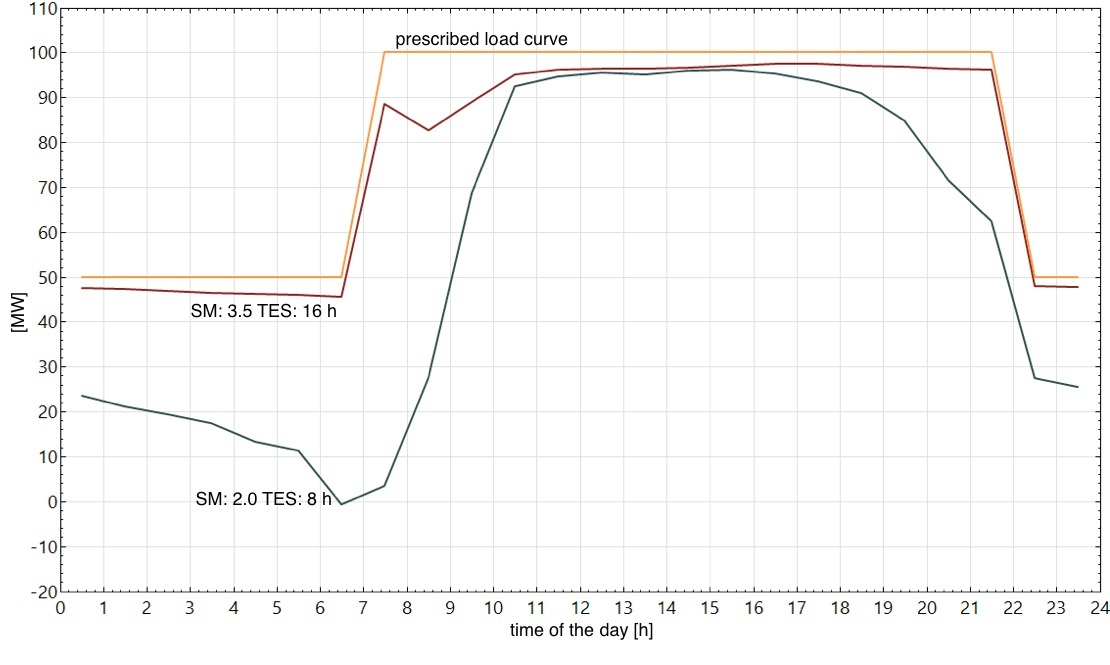
\includegraphics[width=0.8\linewidth]{FIG/CR_annual_profil}
\caption[Annual average load profile of selected CR power plant configurations.]{Annual average load profile of selected CR power plant configurations.}\label{CR_annual_profil}
\end{figure}
Figure~\ref{CR_annual_profil} shows the annual load curve covering of the above mentioned CR power plant high and low configurations with the prescribed load curve. The Figure shows, that the CR power plant using a SM of 3.5 and \SI{16}{h} of TES for the configuration can cover almost at any time of the year the prescribed load curve. The decreasing of the supplied electricity 8:00 leads from the winter duration and will be shown in the following. The lower CR power plant configuration can just cover between 11:00 and 17:00 almost the same amount electricity during the year than the high configuration. In the morning times between 6:00 and 7:00 the energy production is coming to standstill the whole year. The results of all annual average load profiles can be found in Appendix~\ref{all_load_profile}.

At this point it might be necessary to remind, that it is just the electricity used for the annual load covering as well as for the LCOE calculation which is actually supplied at the requested time step. So the electricity which is overproduced at any time of the year is not considered. This can also be seen in Figure~\ref{CR_winter_load}. 
\begin{figure}[htbp]  
\centering
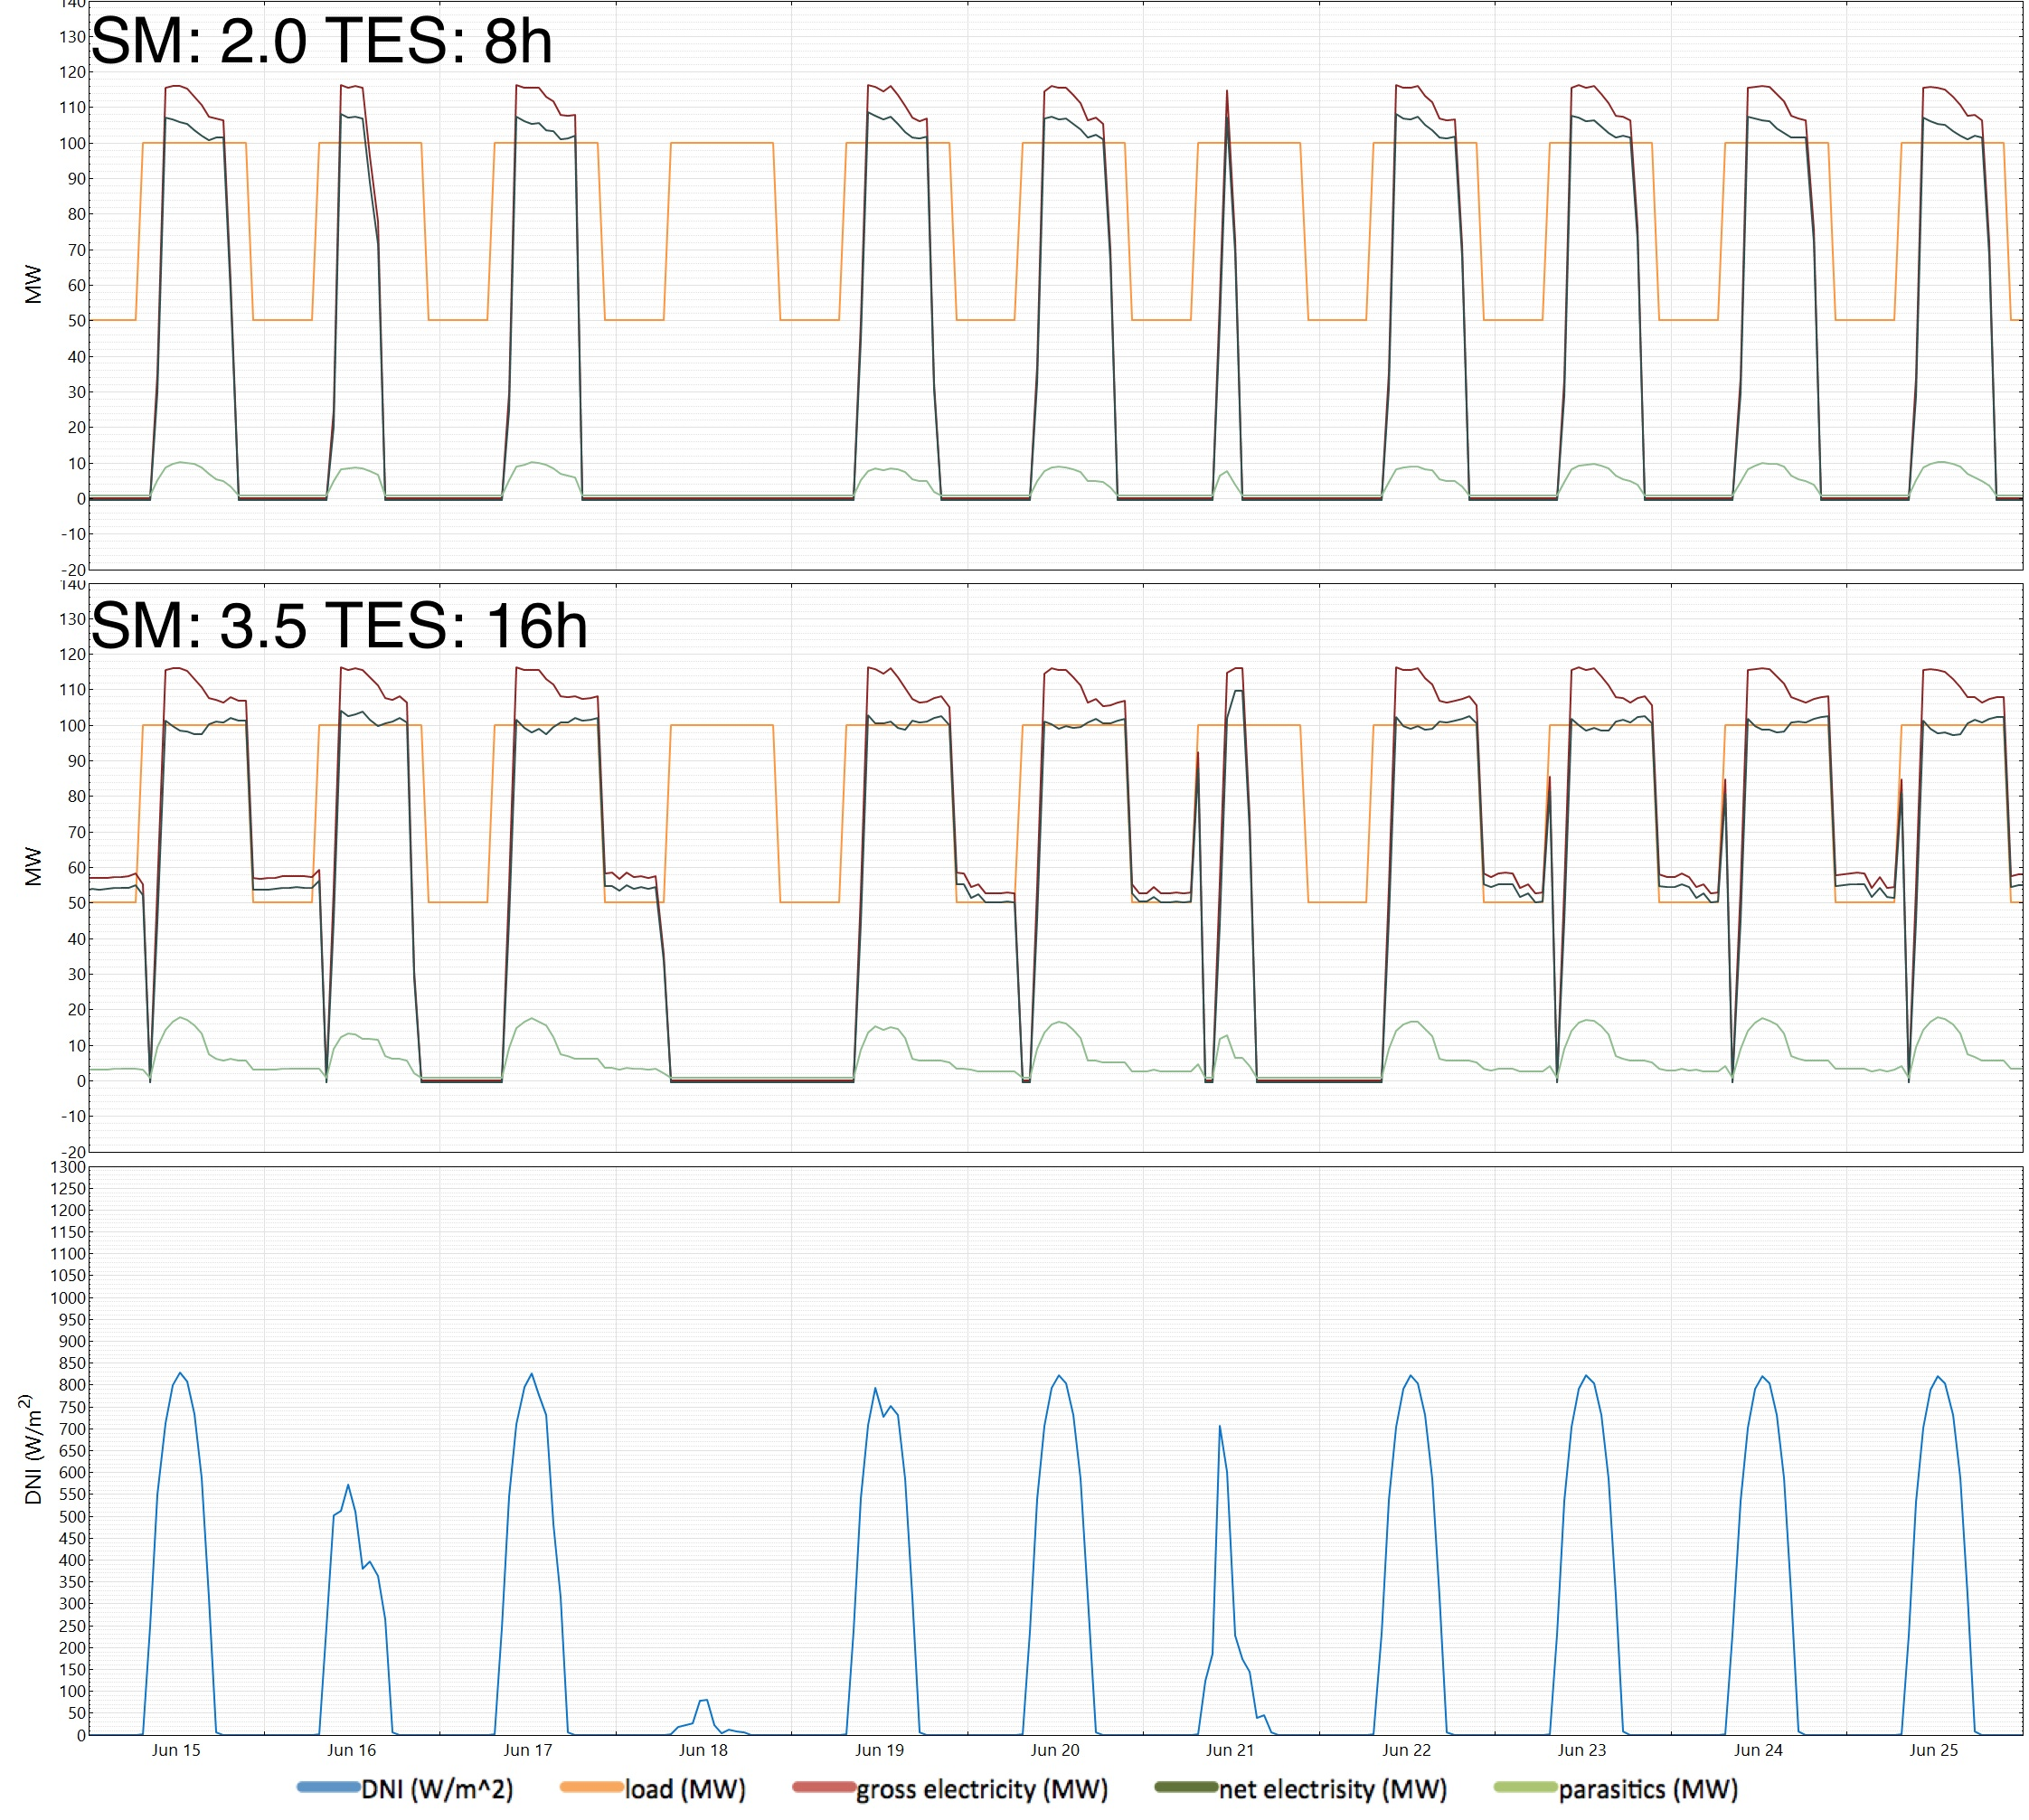
\includegraphics[width=1\linewidth]{FIG/CR_winter_load}
\caption[CR load profile during the time of winter solstice (15. June - 25. June).]{CR load profile during the time of winter solstice (15. June - 25. June).}\label{CR_winter_load}
\end{figure}
This figure shows exemplary the load curve behavior of the CR power plants during the time with the least hours of sunlight during a day of the year. The DNI is around \SI{830}{\watt\per\square\metre} in peak times at these days and there are also days with less or almost no direct irradiance. As mentioned, it can be seen that the net electricity production is in both cases at some times across the prescribed load curve and is not consulted further. This reaches mainly from the described dispatch control matrix from Figure~\ref{CR_turbineoutput} on Page~\pageref{CR_turbineoutput} to control the turbine output. This is not accurate at all to follow a specific load exactly during each day of the year. 

However, Figure~\ref{CR_winter_load} mainly shows the load curve behavior of the CR power plants in low and high configuration. At a SM of \si{2.0} with \SI{8}{h} of TES the power plant can't produce enough power during the day to fill up the TES for generating power during the night. Compared to that, the CR power plant with a SM of \si{3.5} and \SI{16}{h} of TES can almost anytime generate electricity over the whole night. But with the rising load in the morning hours the energy production stops due to the empty storage. 
\begin{figure}[htbp]  
\centering
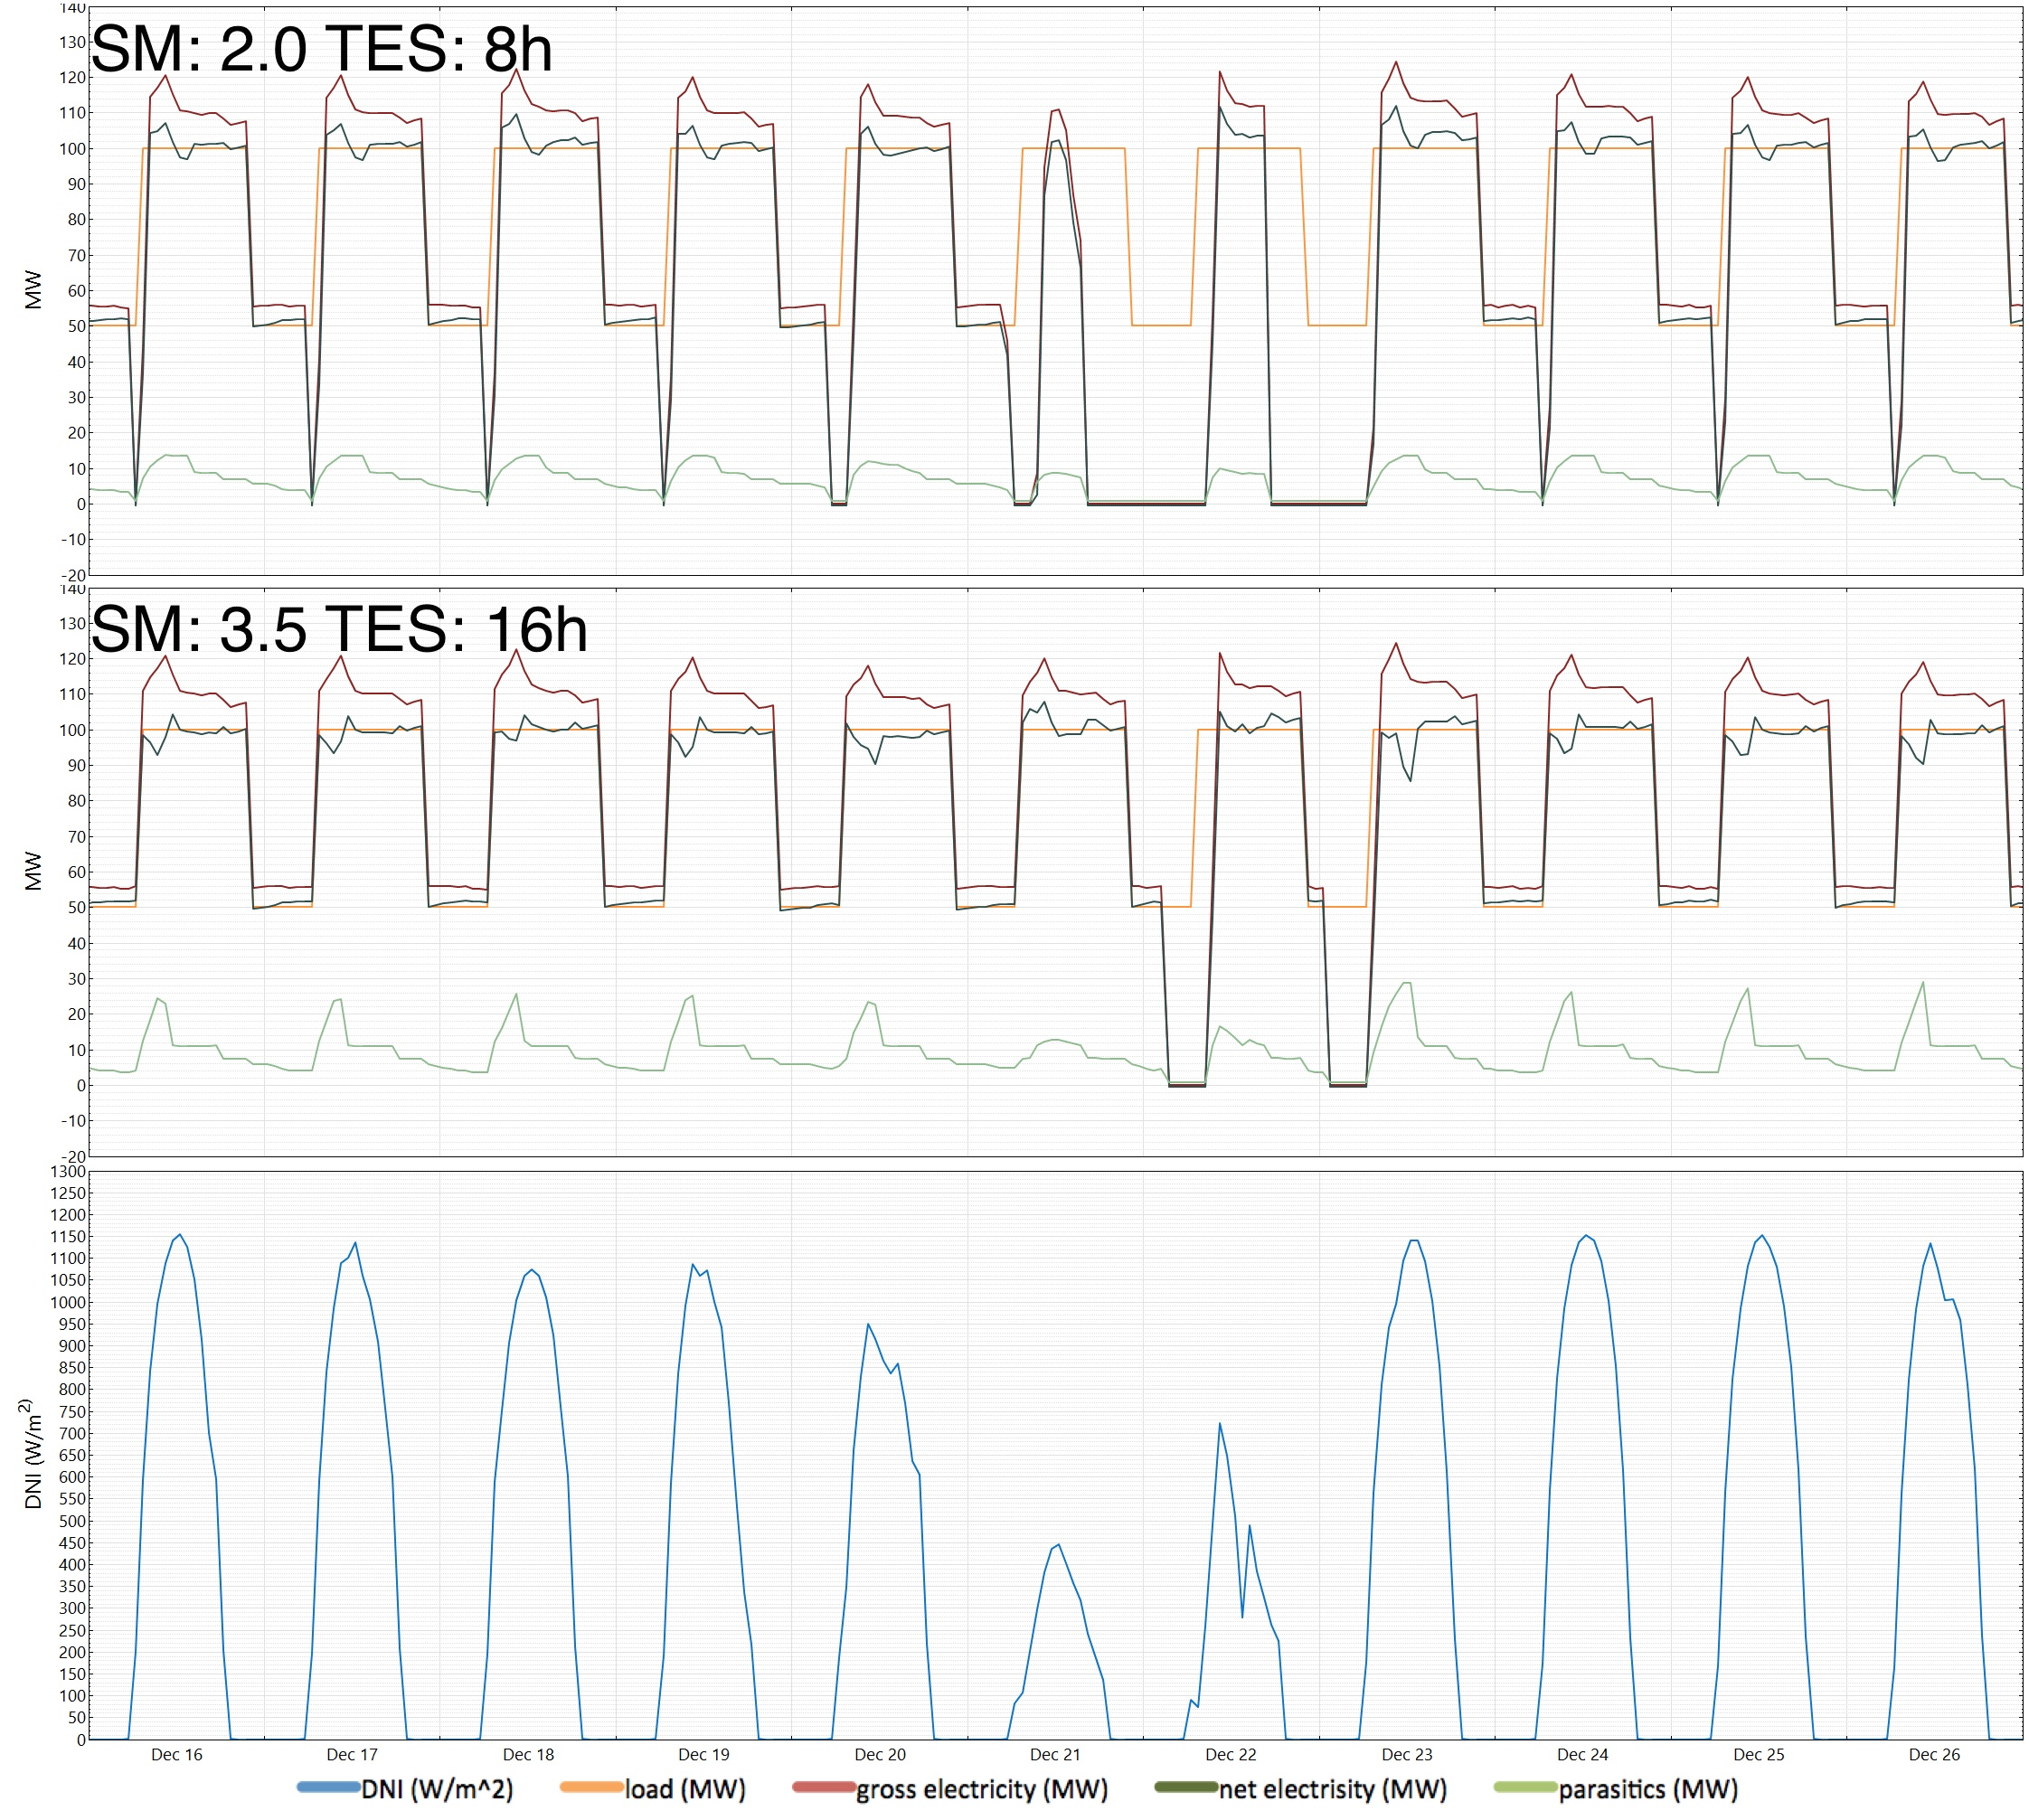
\includegraphics[width=1\linewidth]{FIG/CR_summer_load}
\caption[CR load profile during the time of summer solstice (16. December - 26. December).]{CR load profile during the time of summer solstice (16. December - 26. December).}\label{CR_summer_load}
\end{figure}
This leads also to the above mentioned decreasing in supply at \SI{8}{am} in the annual average load profile. The difference between the gross and net electricity production is coming from the parasitic consume within the power plant.

Figure~\ref{CR_summer_load} describes the load behavior of the  same power plants during the longest days of the year. It is clearly to see, that the irradiation is higher and longer during the days compare to the winter solstice. The peaks of DNI are about 1~\SI{150}{\watt\per\square\metre} during that days. At a SM of 2.0 and \SI{8}{h} of TES the CR power plant is not able to follow the prescribed electricity load over the whole day. It's coming to standstill between 6 and \SI{7}{am} at least. Therefrom also the annual average load profile is coming to stand still at these time of the day. The CR power plant with a SM of 3.5 and \SI{16}{h} of TES can follow the prescribed load mostly without any problems. Outstanding for the high productivity of the plant configuration is the electricity output while having low direct irradiance. At the 21. of December the plant can supply almost the whole prescribed load using reserves from the TES.

A detailed look to the parasitic behaviors of the CR power plant with a SM of \si{3.5} and \SI{16}{h} of TES reveals a strong decreasing after a moderate increasing during the midday. This happens when the storage is full loaded and the steam turbine don't need more power. At this point a specified amount of heliostats defocusing the receiver and the power of the receivers HTF pump is getting reduced. 

\begin{figure}[!htbp]
        \centering   
        \begin{subfigure}[b]{0.65\textwidth}
                \centering
                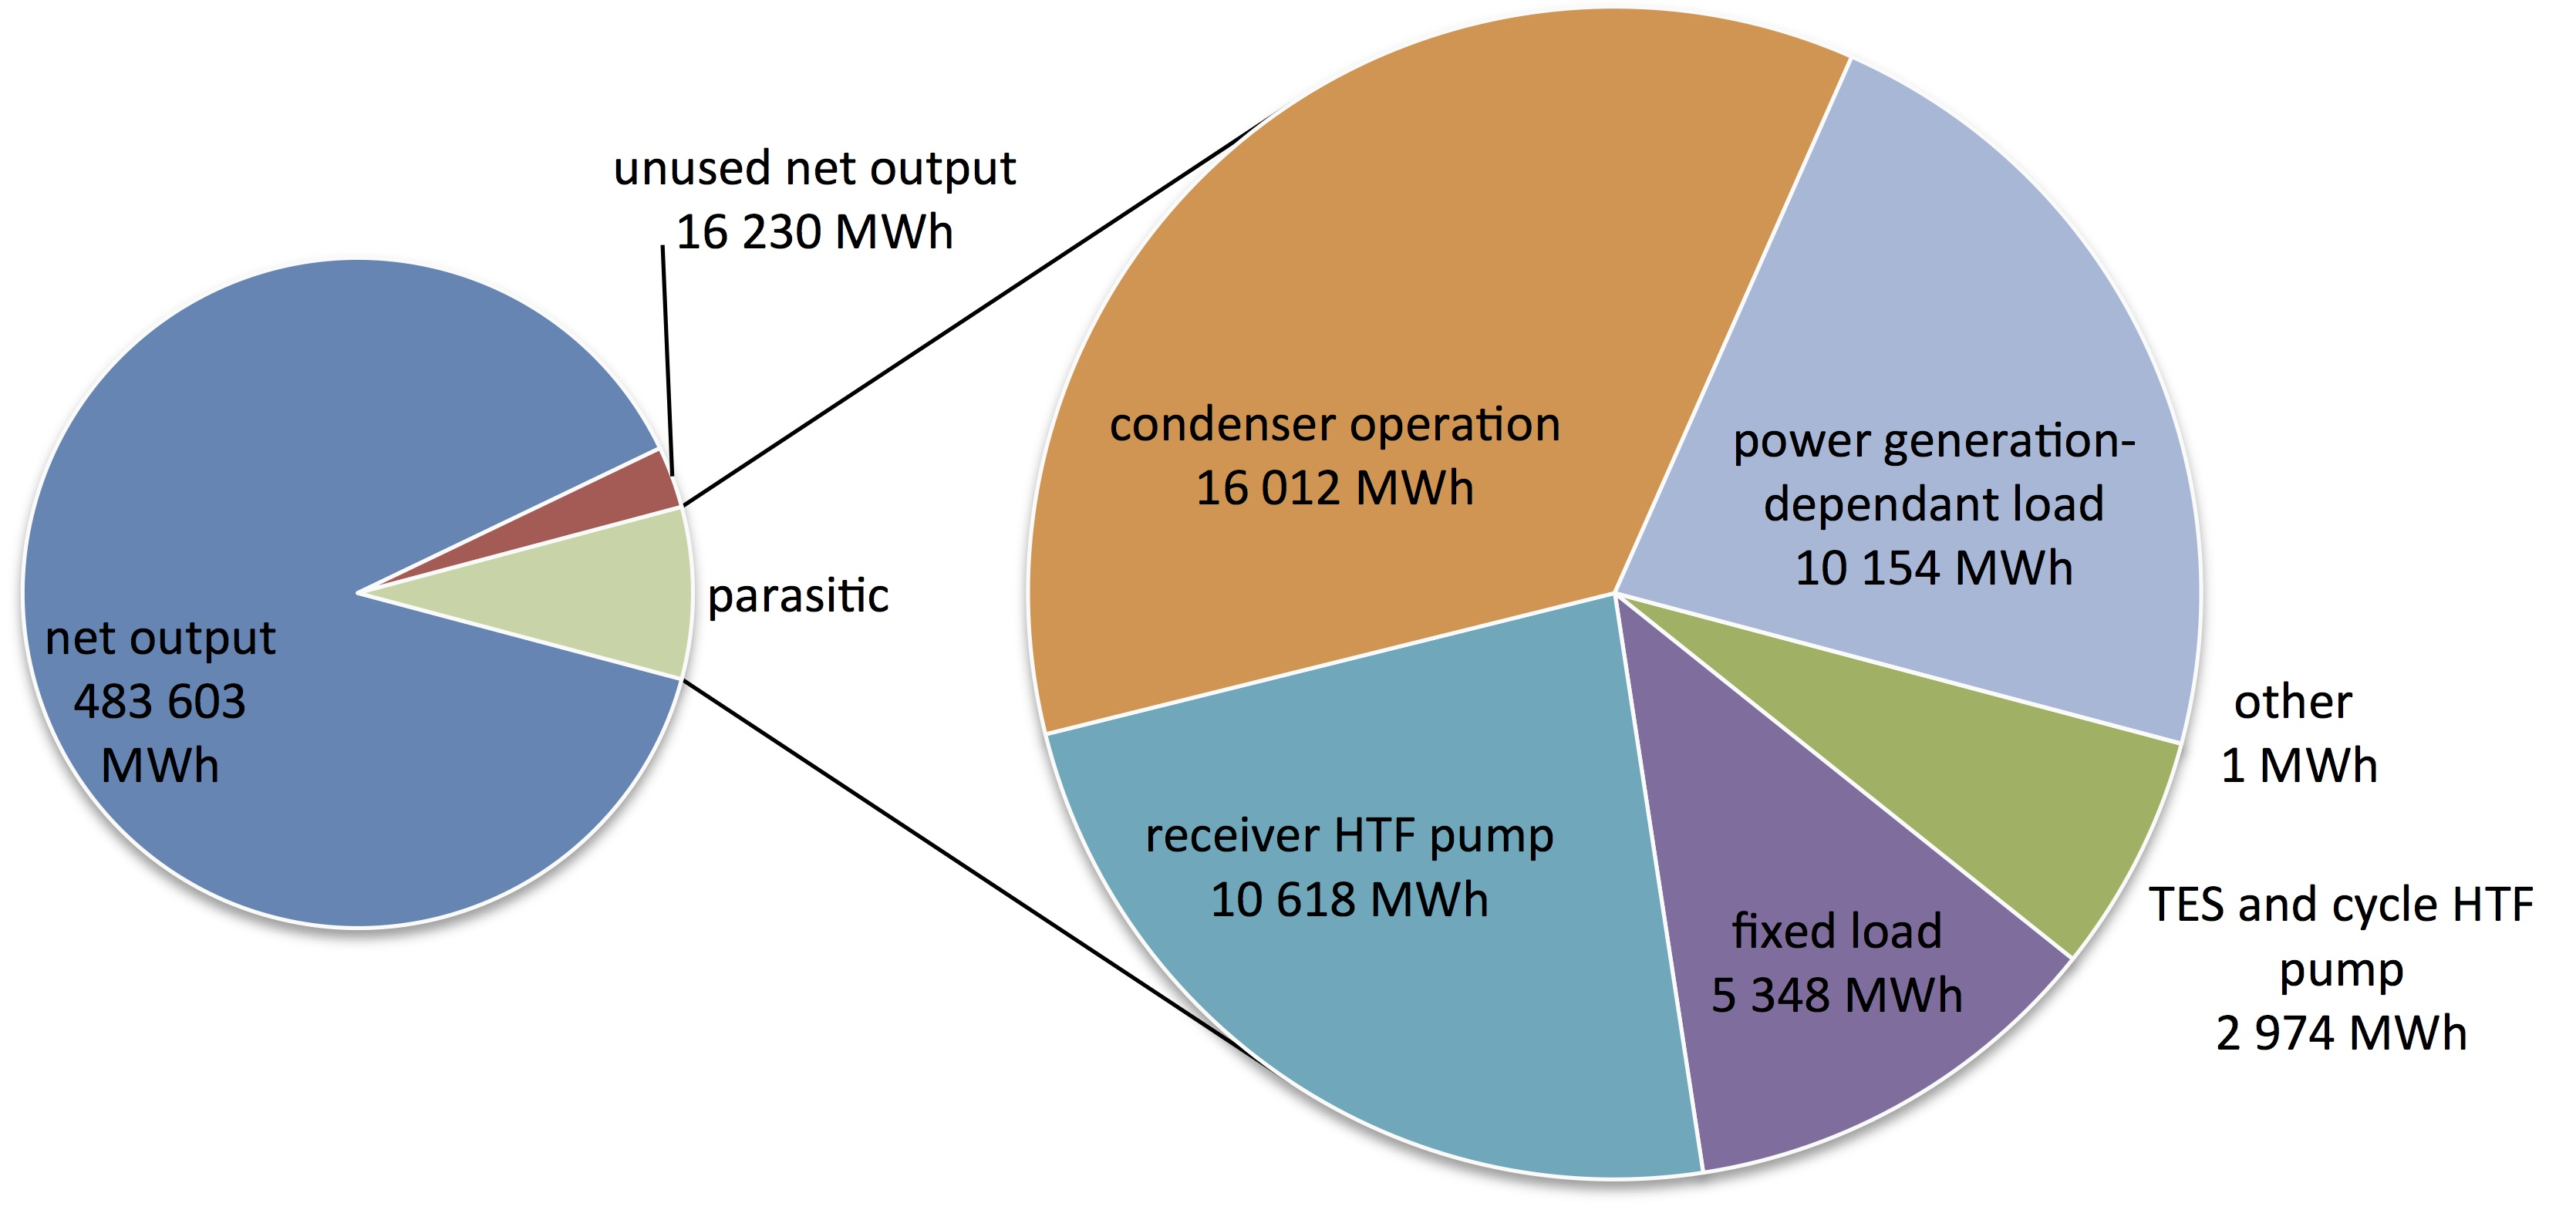
\includegraphics[width=1\textwidth]{FIG/CR_parasitics_low}
                \caption{SM: 2.0 TES: 8 h}\label{CR_parasitics_low}
        \end{subfigure}
\par\medskip % Linebreak              
        \begin{subfigure}[b]{0.65\textwidth}
                \centering
                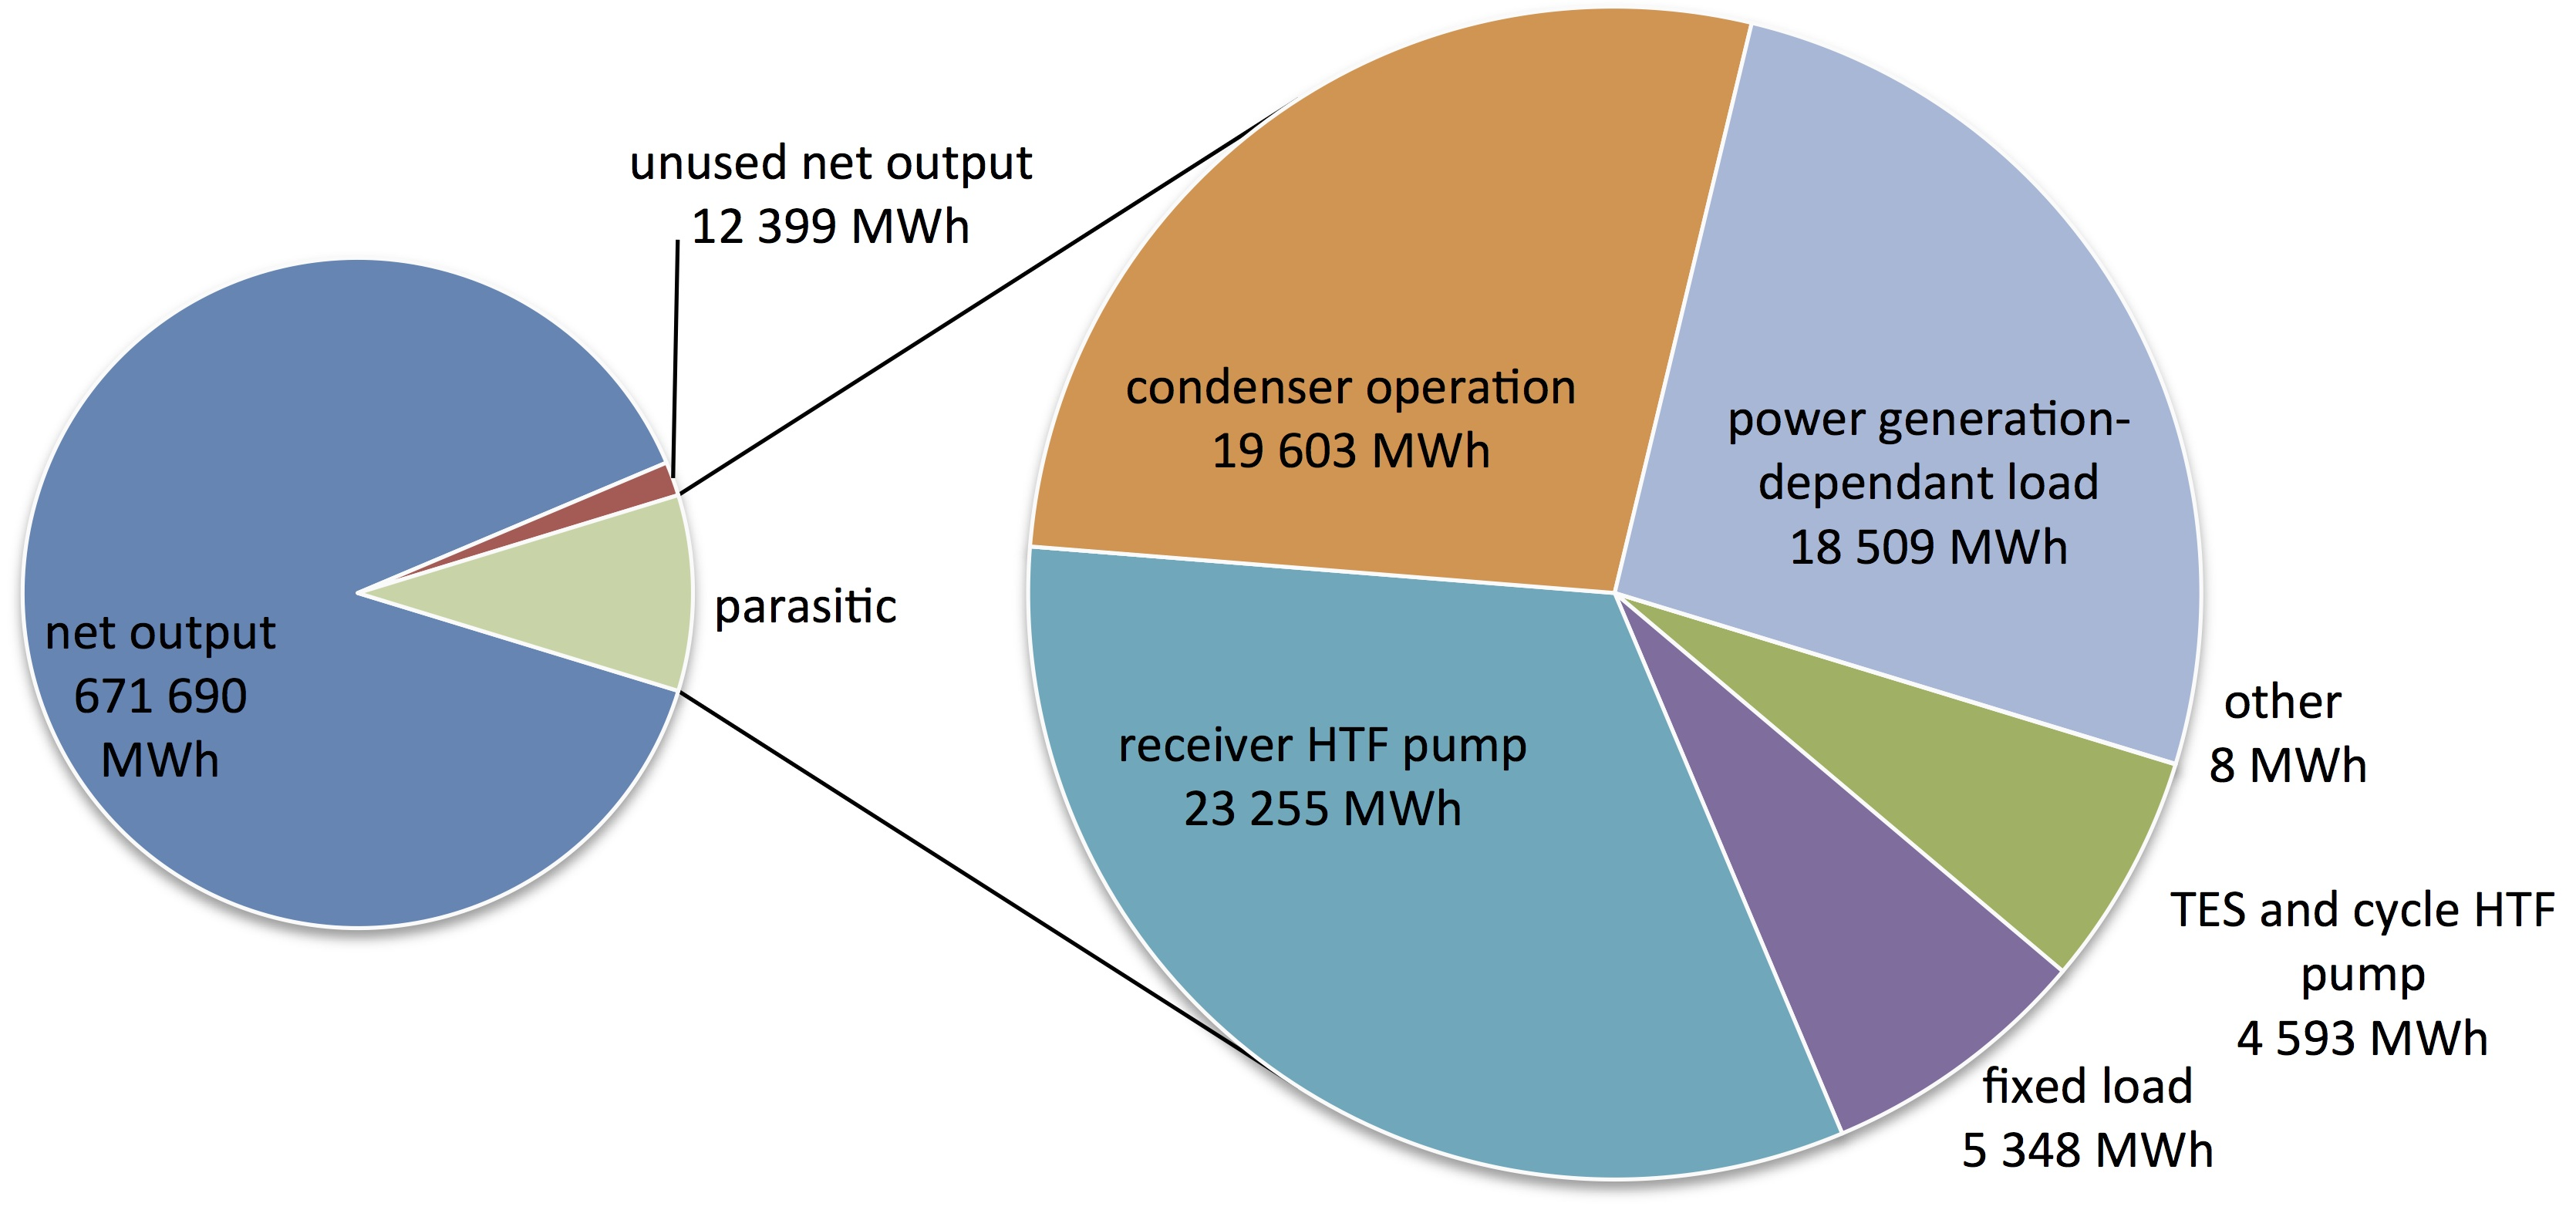
\includegraphics[width=1\textwidth]{FIG/CR_parasitics_high}
                \caption{SM: 3.5 TES: 16 h}\label{CR_parasitics_high}
        \end{subfigure}
        \caption[Share of annual gross energy output of selected CR power plant configurations.]{Share of annual gross energy output of selected CR power plant configurations.}\label{CR_parasitics}
\end{figure}
The parasitic load is composed from various electrical loads of the power plant, namely pumping loads, cooling loads, fixed loads and loads depending from the power generation. The share of these electrical parasitic loads and the total share of the gross energy output of the selected CR power plans can be seen in Figure~\ref{CR_parasitics}. The share of the net energy production out of the gross energy production is about 90~\%. The unused net energy output share of all simulated CR power plants is between 1.6 and 3.2~\% and went not into the LCOE calculation.

Figure~\ref{CR_parasitics_low} shows, that the net outputs share of the lowest CR power plant configuration is about \SI{483.60}{GWh}.  The total sum of the annual prescribed load is \SI{711.75}{GWh}. So the power plant covers the prescribed load for 67.9~\%. The net outputs share of the highest CR power plant configuration from Figure~\ref{CR_parasitics_high} is \SI{671.69}{GWh} and is covering the prescribed load for 94.4~\% over the year.

Figure~\ref{CR_LCCF} summarizes the results of the load curve covering for all simulated CR configurations. The chart shows that at a SM of 2.0 all TES variations besides \SI{8}{h} a covering more than 70~\% of the prescribed load. At a SM of 2.5 the and a TES about \SI{10}{h} the results showed over 80~\% load covering. A load curve covering of about 90~\% is reached at a SM of 3.0 and more than \SI{14}{h} of TES. The configuration with a \SI{12}{h} TES reaches just 89.1~\% at a SM of 3.0. 

\begin{figure}[htbp]  
\centering
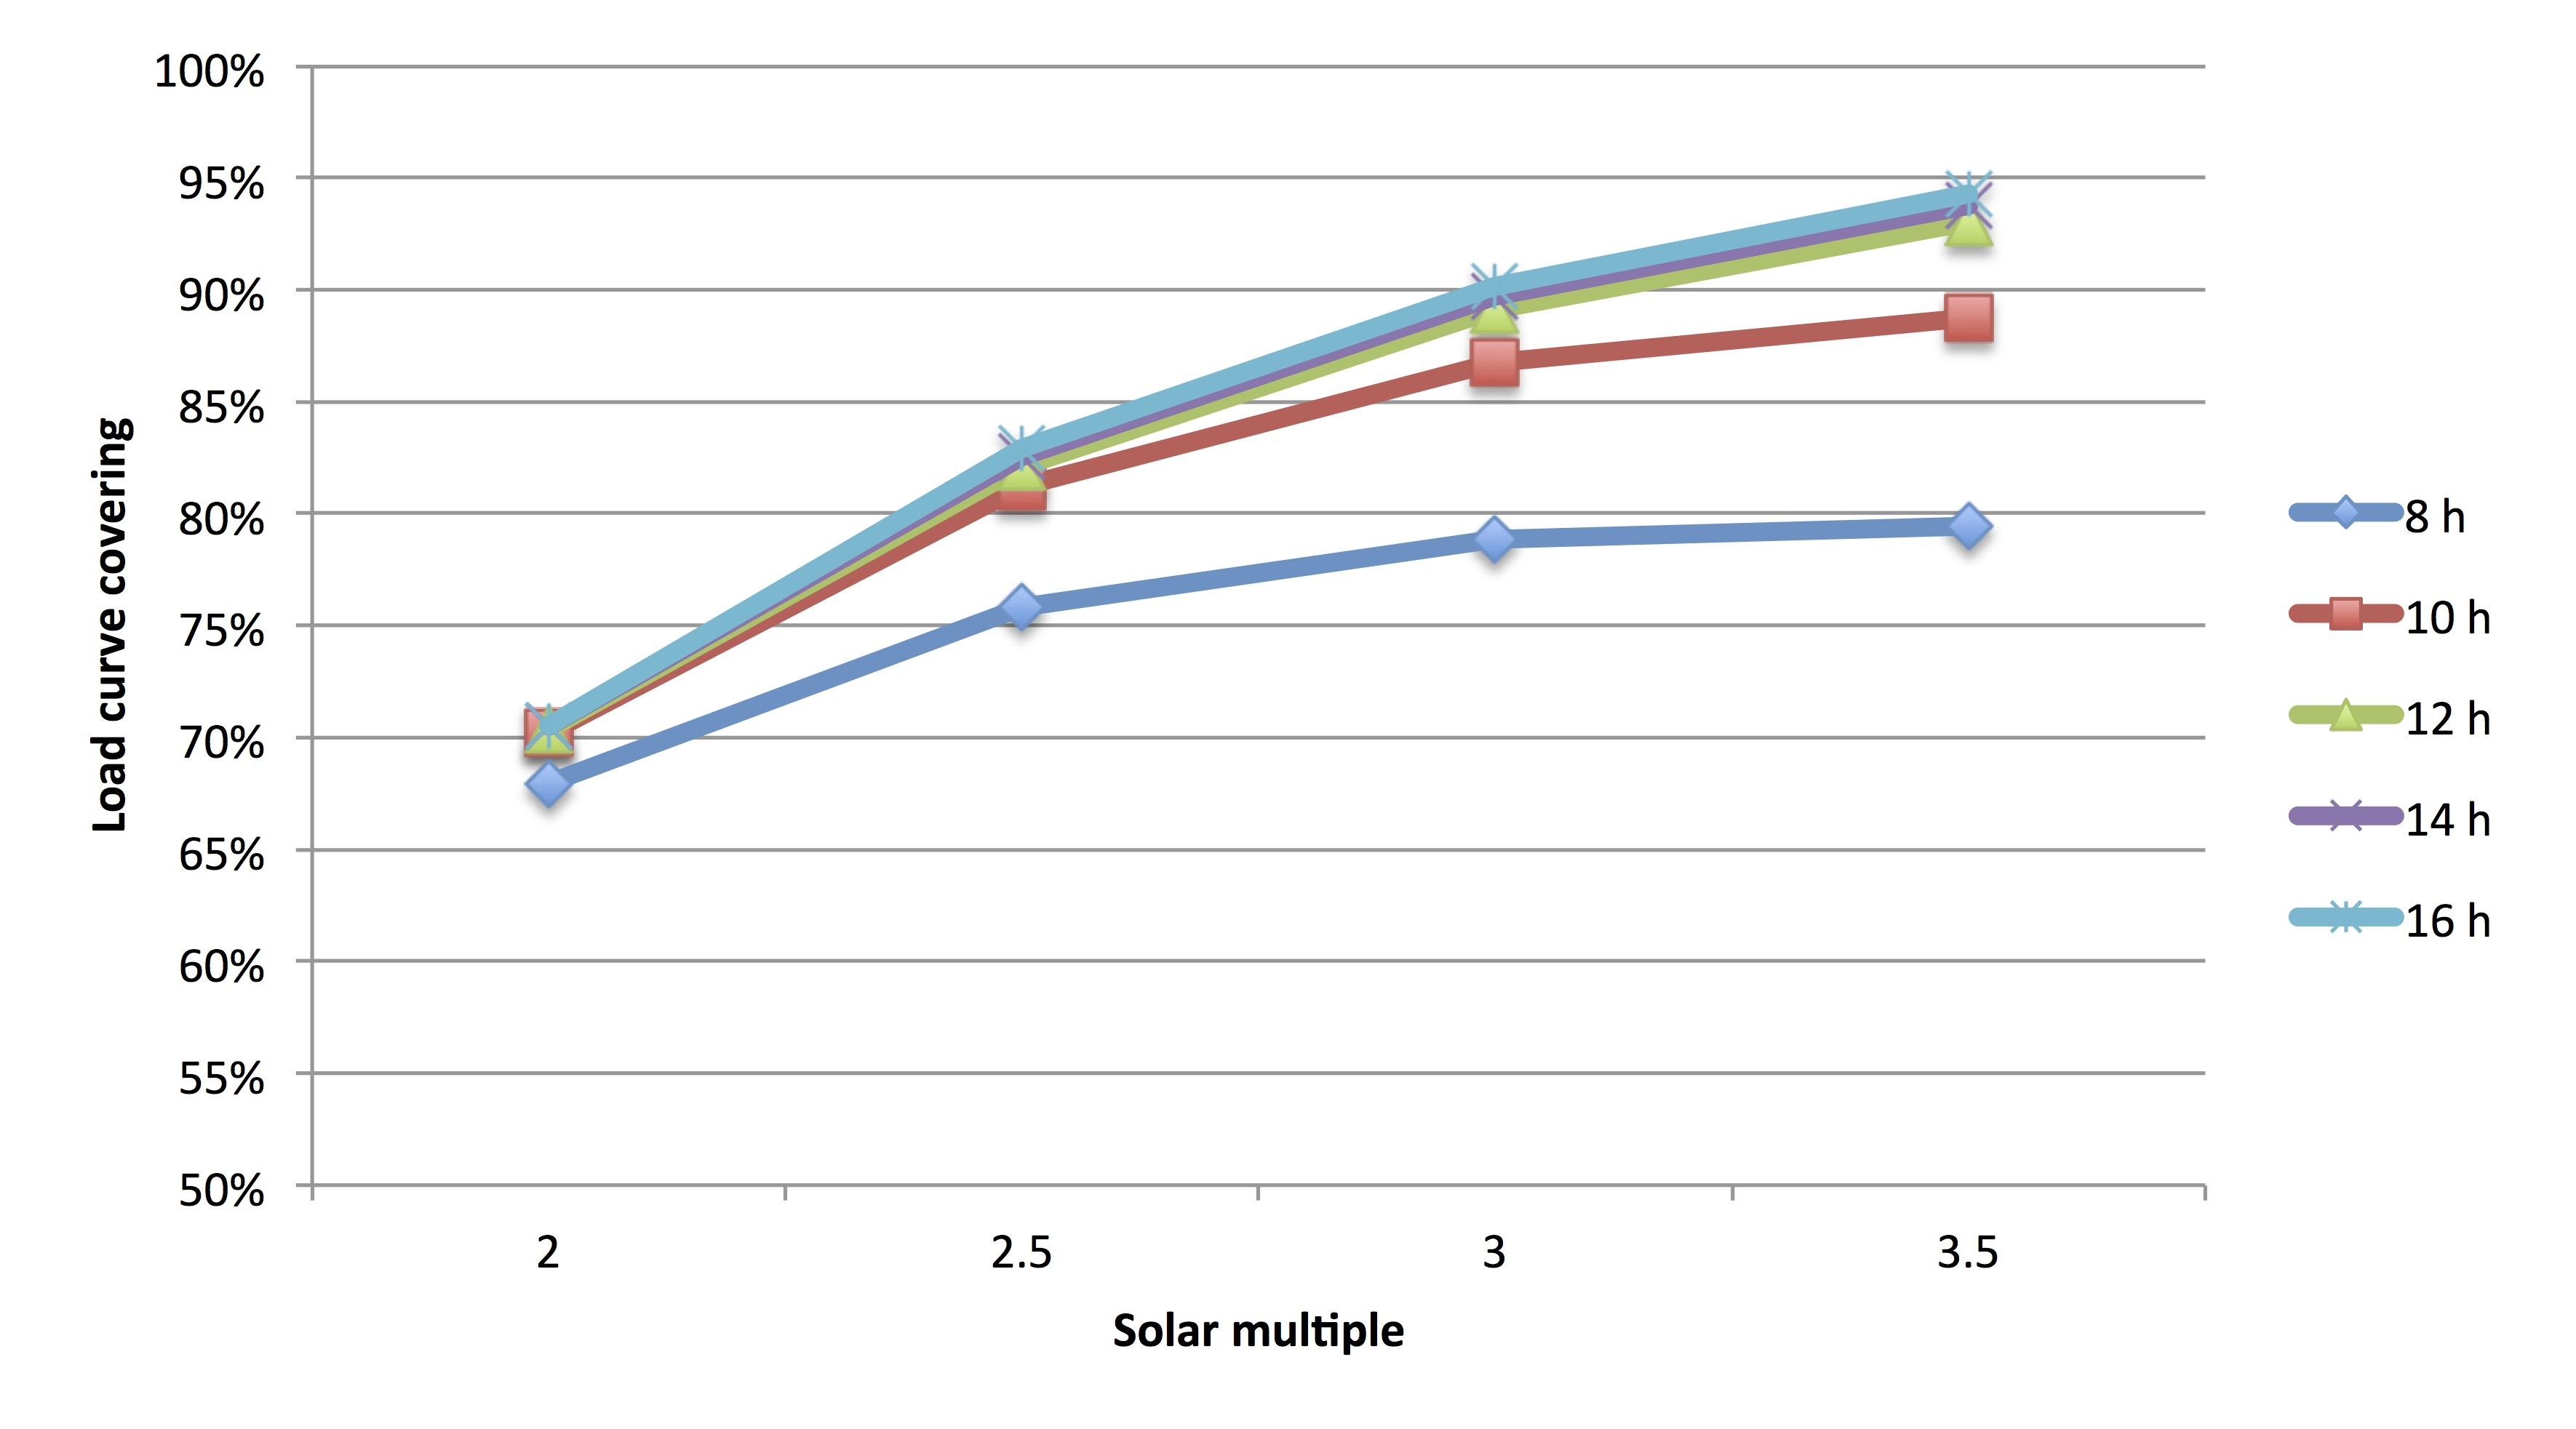
\includegraphics[width=1\linewidth]{FIG/CR_LCCF}
\caption[Load curve covering result of simulated CR systems.]{Load curve covering result of simulated CR systems.}\label{CR_LCCF}
\end{figure}
The results of the load curve covering shows that there is no appreciable difference between the 12, 14 and \SI{16}{h} of TES. At a SM of 3.5 the difference is just 1.4~\% load curve covering between 12 and \SI{16}{h} of TES. There is just a addition of 0.6~\% for the \SI{8}{h} TES and the SM 3.0 to 3.5 configurations. 
\subsubsection{Levelized costs of electricity}
The results of the LCOE claculation for the simulated CR configurations can be seen in Figure~\ref{CR_LCOE}. They are calculated using the finacial input parameter in Table~\ref{tbl: CRFinance} and a simplified method which is documented in Appendix~\ref{ChapterLCOE} on Page \pageref{ChapterLCOE}.

\begin{figure}[htbp]  
\centering
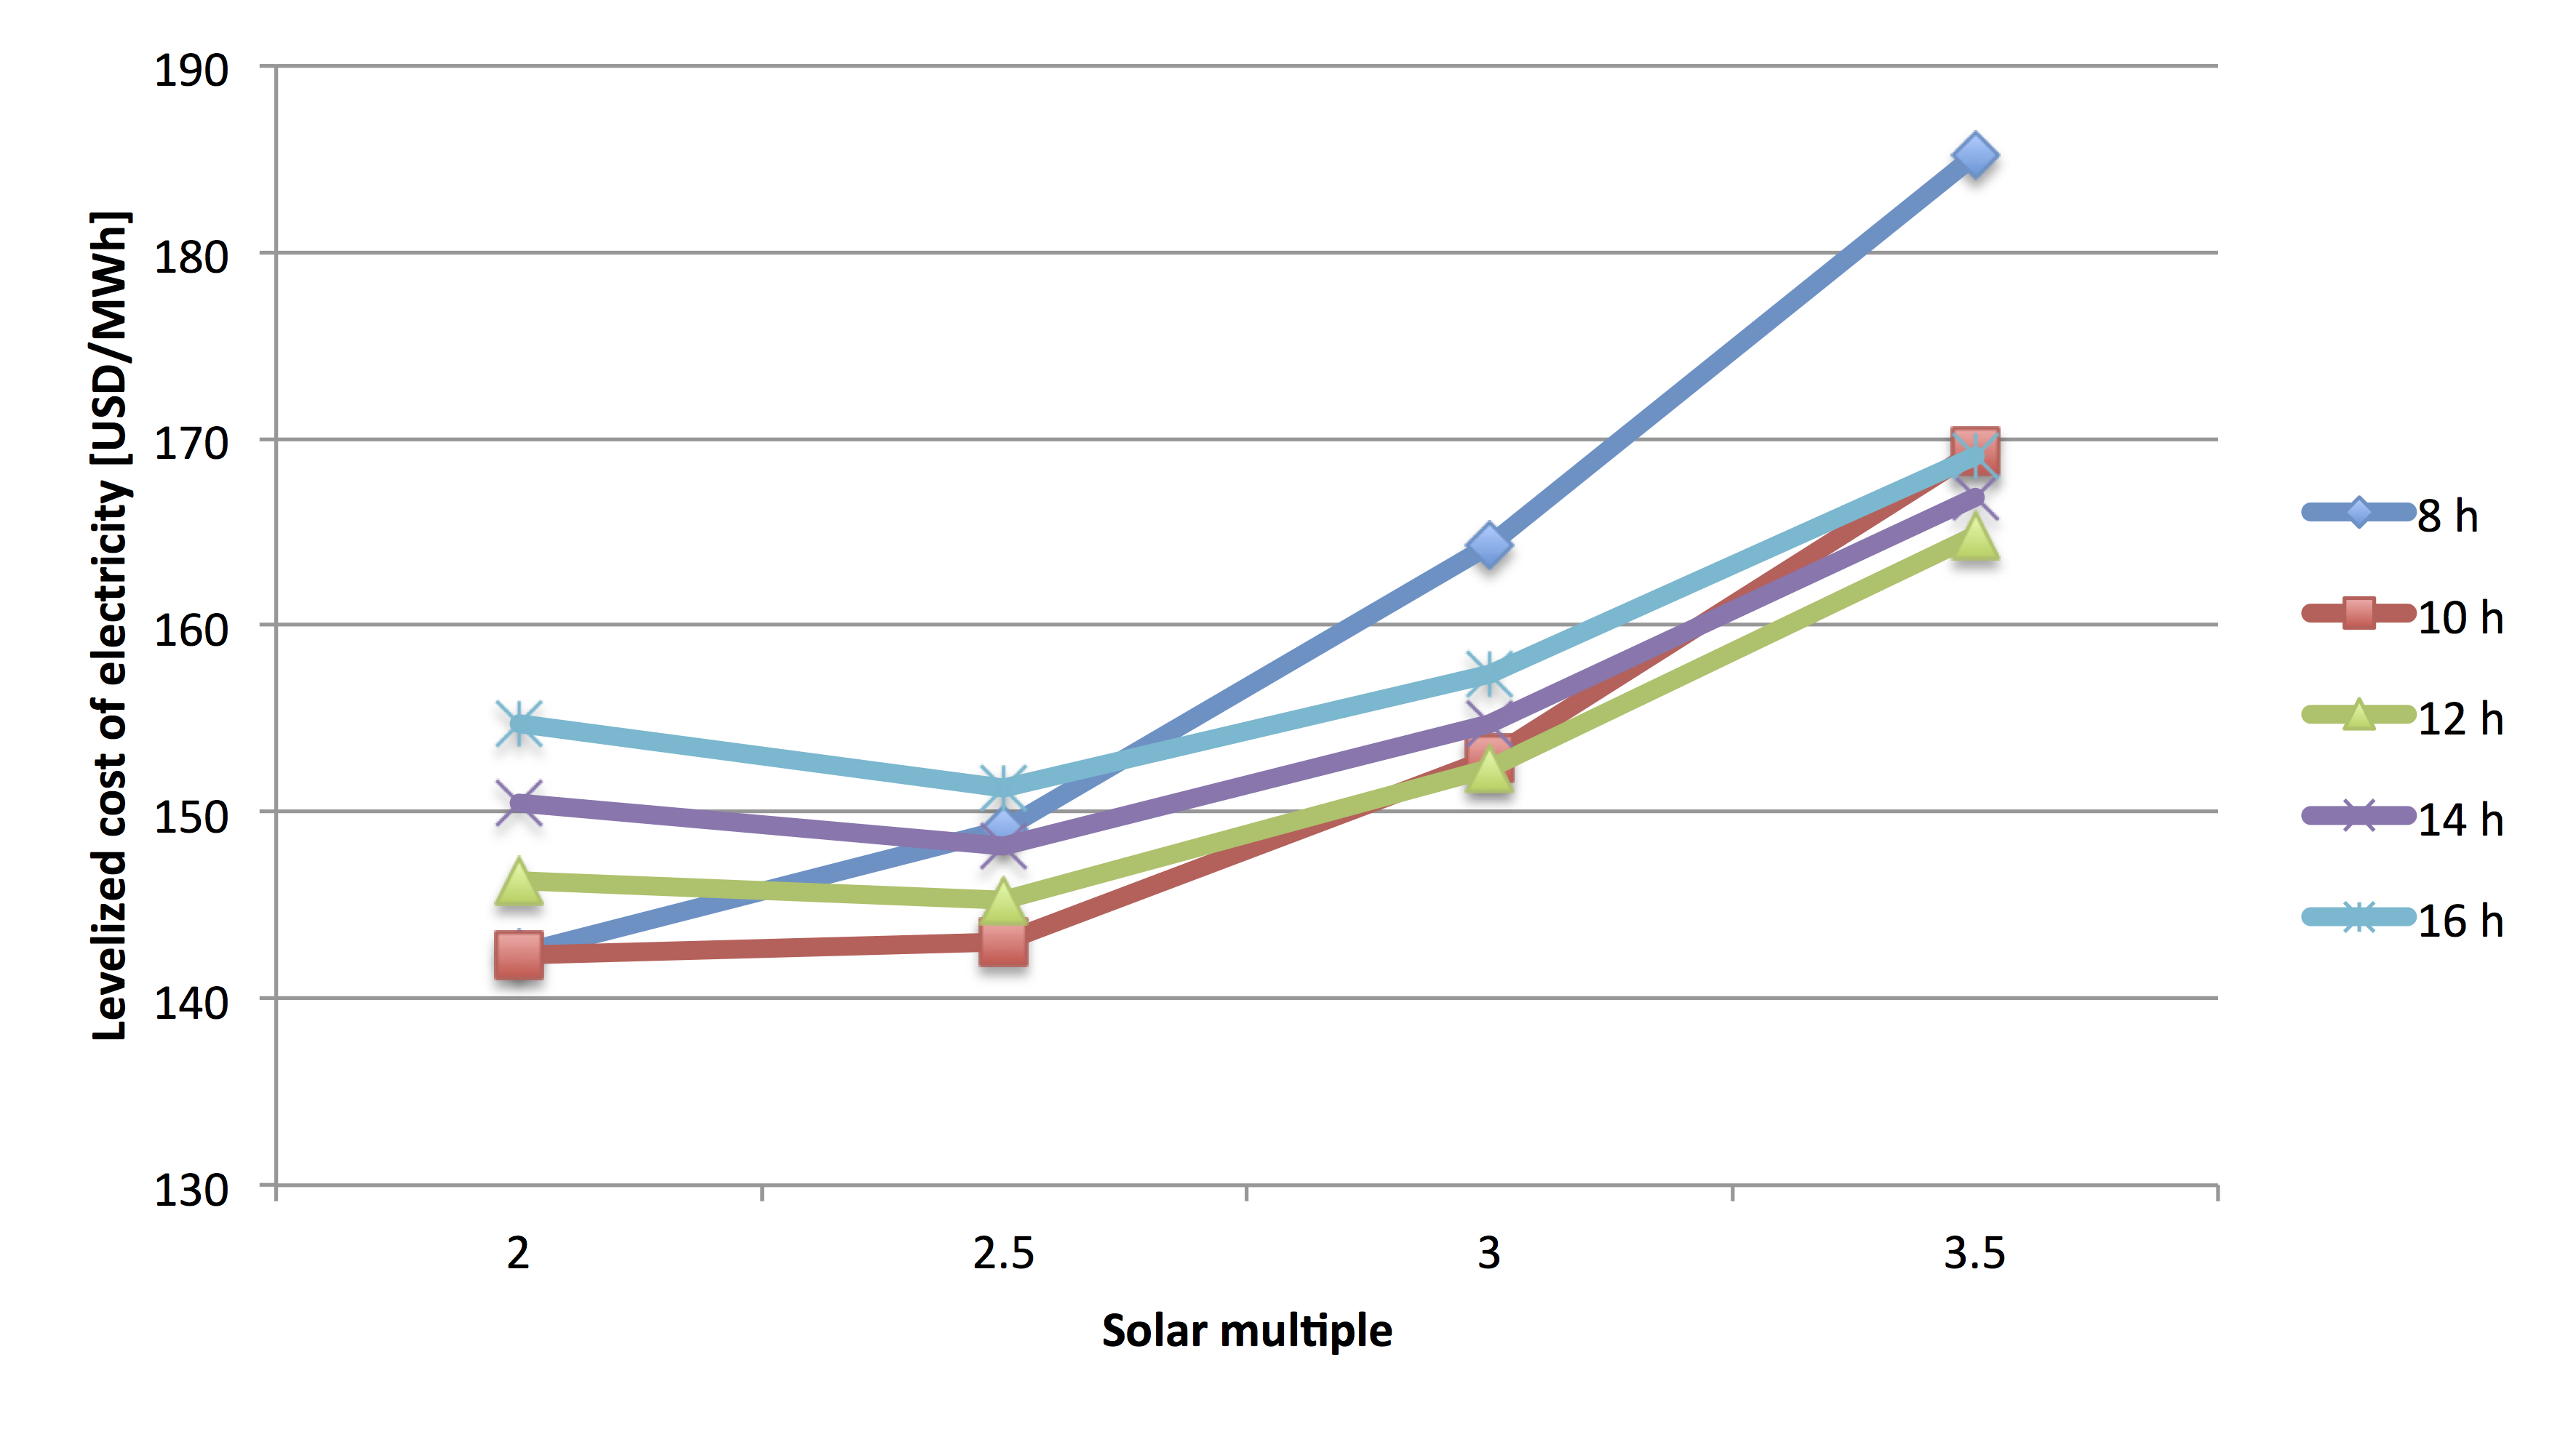
\includegraphics[width=1\linewidth]{FIG/CR_LCOE}
\caption[LCOE calculation results for CR simulation.]{LCOE calculation results for CR simulation.}\label{CR_LCOE}
\end{figure}
The results of the calculation shows that the lowest LCOE of \SI{137.55}{USD/MWh} is reached at a SM of 2.0 and \SI{10}{h} of TES and is just  marginal cheaper then using \SI{8}{h} of TES with a LCOE of \SI{137.63}{USD/MWh}. The LCOE addition from SM 2.0 to 2.5 is goes minimal up to \SI{138.25}{USD/MWh} for \SI{10}{h} of TES. The highest LCOE result of the simulated configurations is 179.00~\$cent/kWh at a SM of 3.5 and \SI{8}{h} of TES. 

The behavior of the 12, 14 and \SI{16}{h} of TES results for all SM of the LCOE is almost identical. Just the individual value is differently.

\begin{figure}[!htbp]
        \centering                
        \begin{subfigure}[b]{0.5\textwidth}
                \centering
                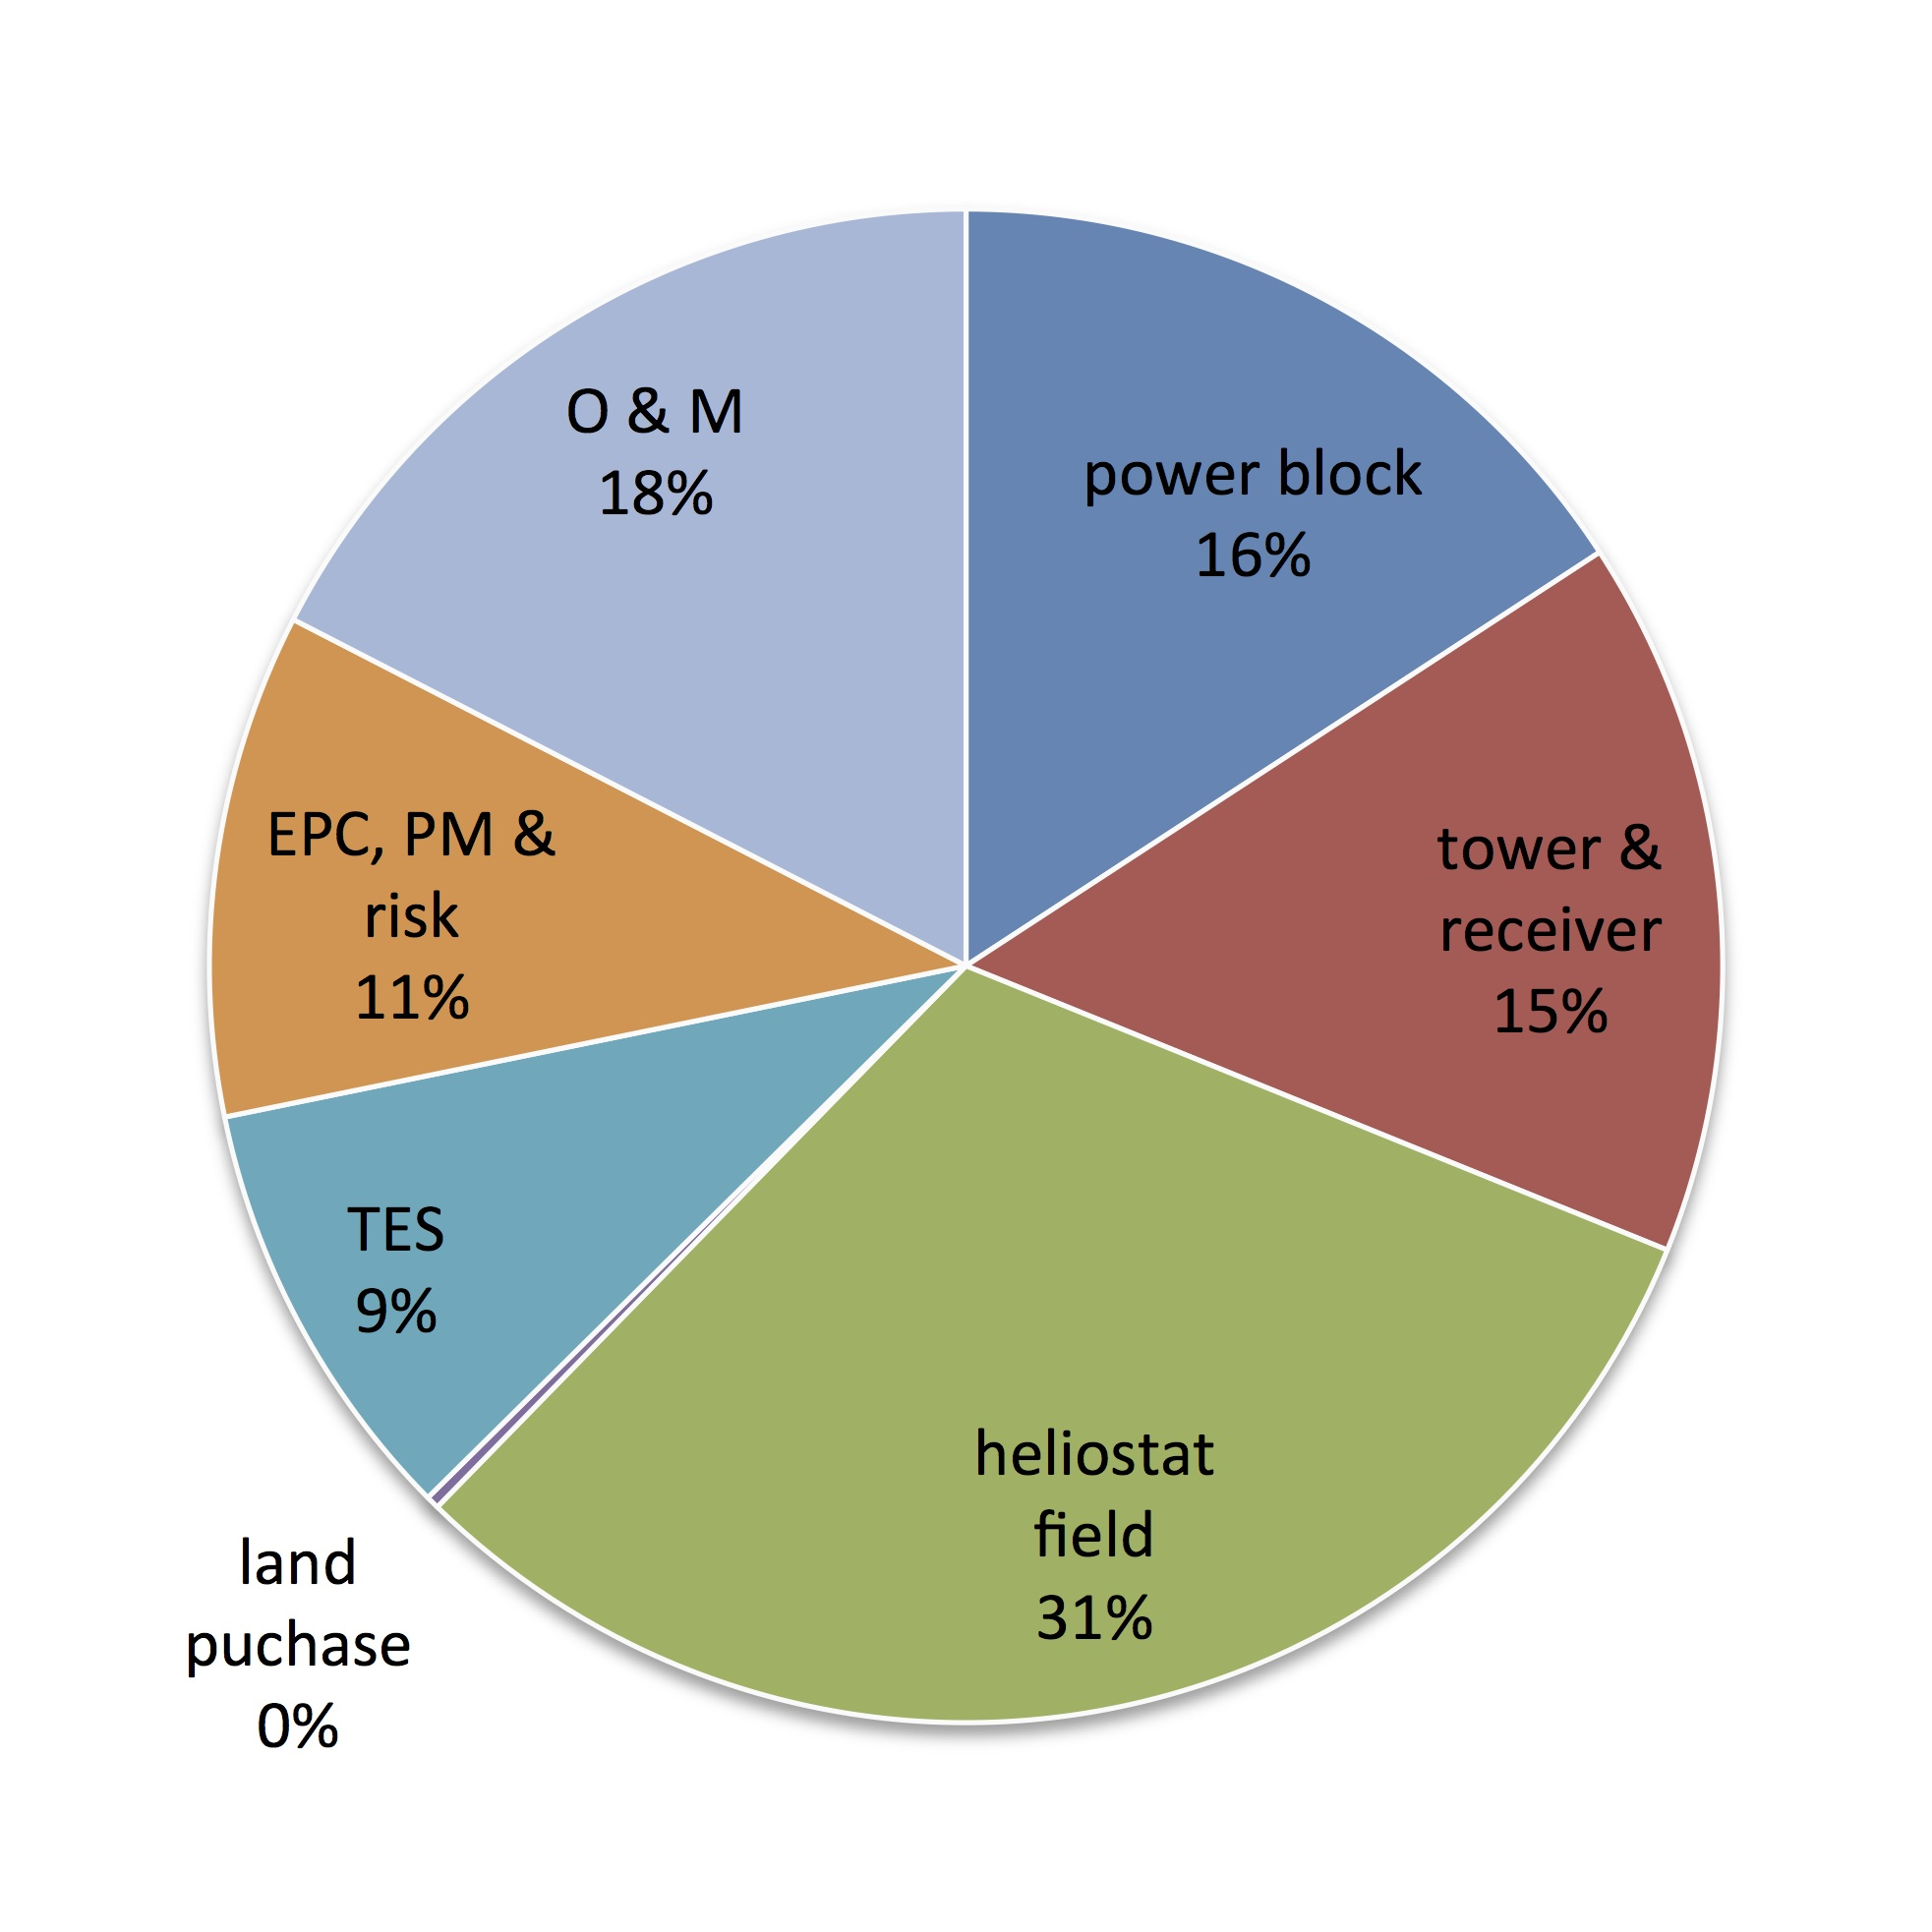
\includegraphics[width=1\textwidth]{FIG/CR_LCOE_lowinvest_BreakDown}
                \caption{LCOE break-down for SM~2.0 and \SI{8}{h}~TES.}\label{CR_LCOE_lowinvest_BreakDown}
        \end{subfigure}%
        ~
        \begin{subfigure}[b]{0.5\textwidth}
                \centering
                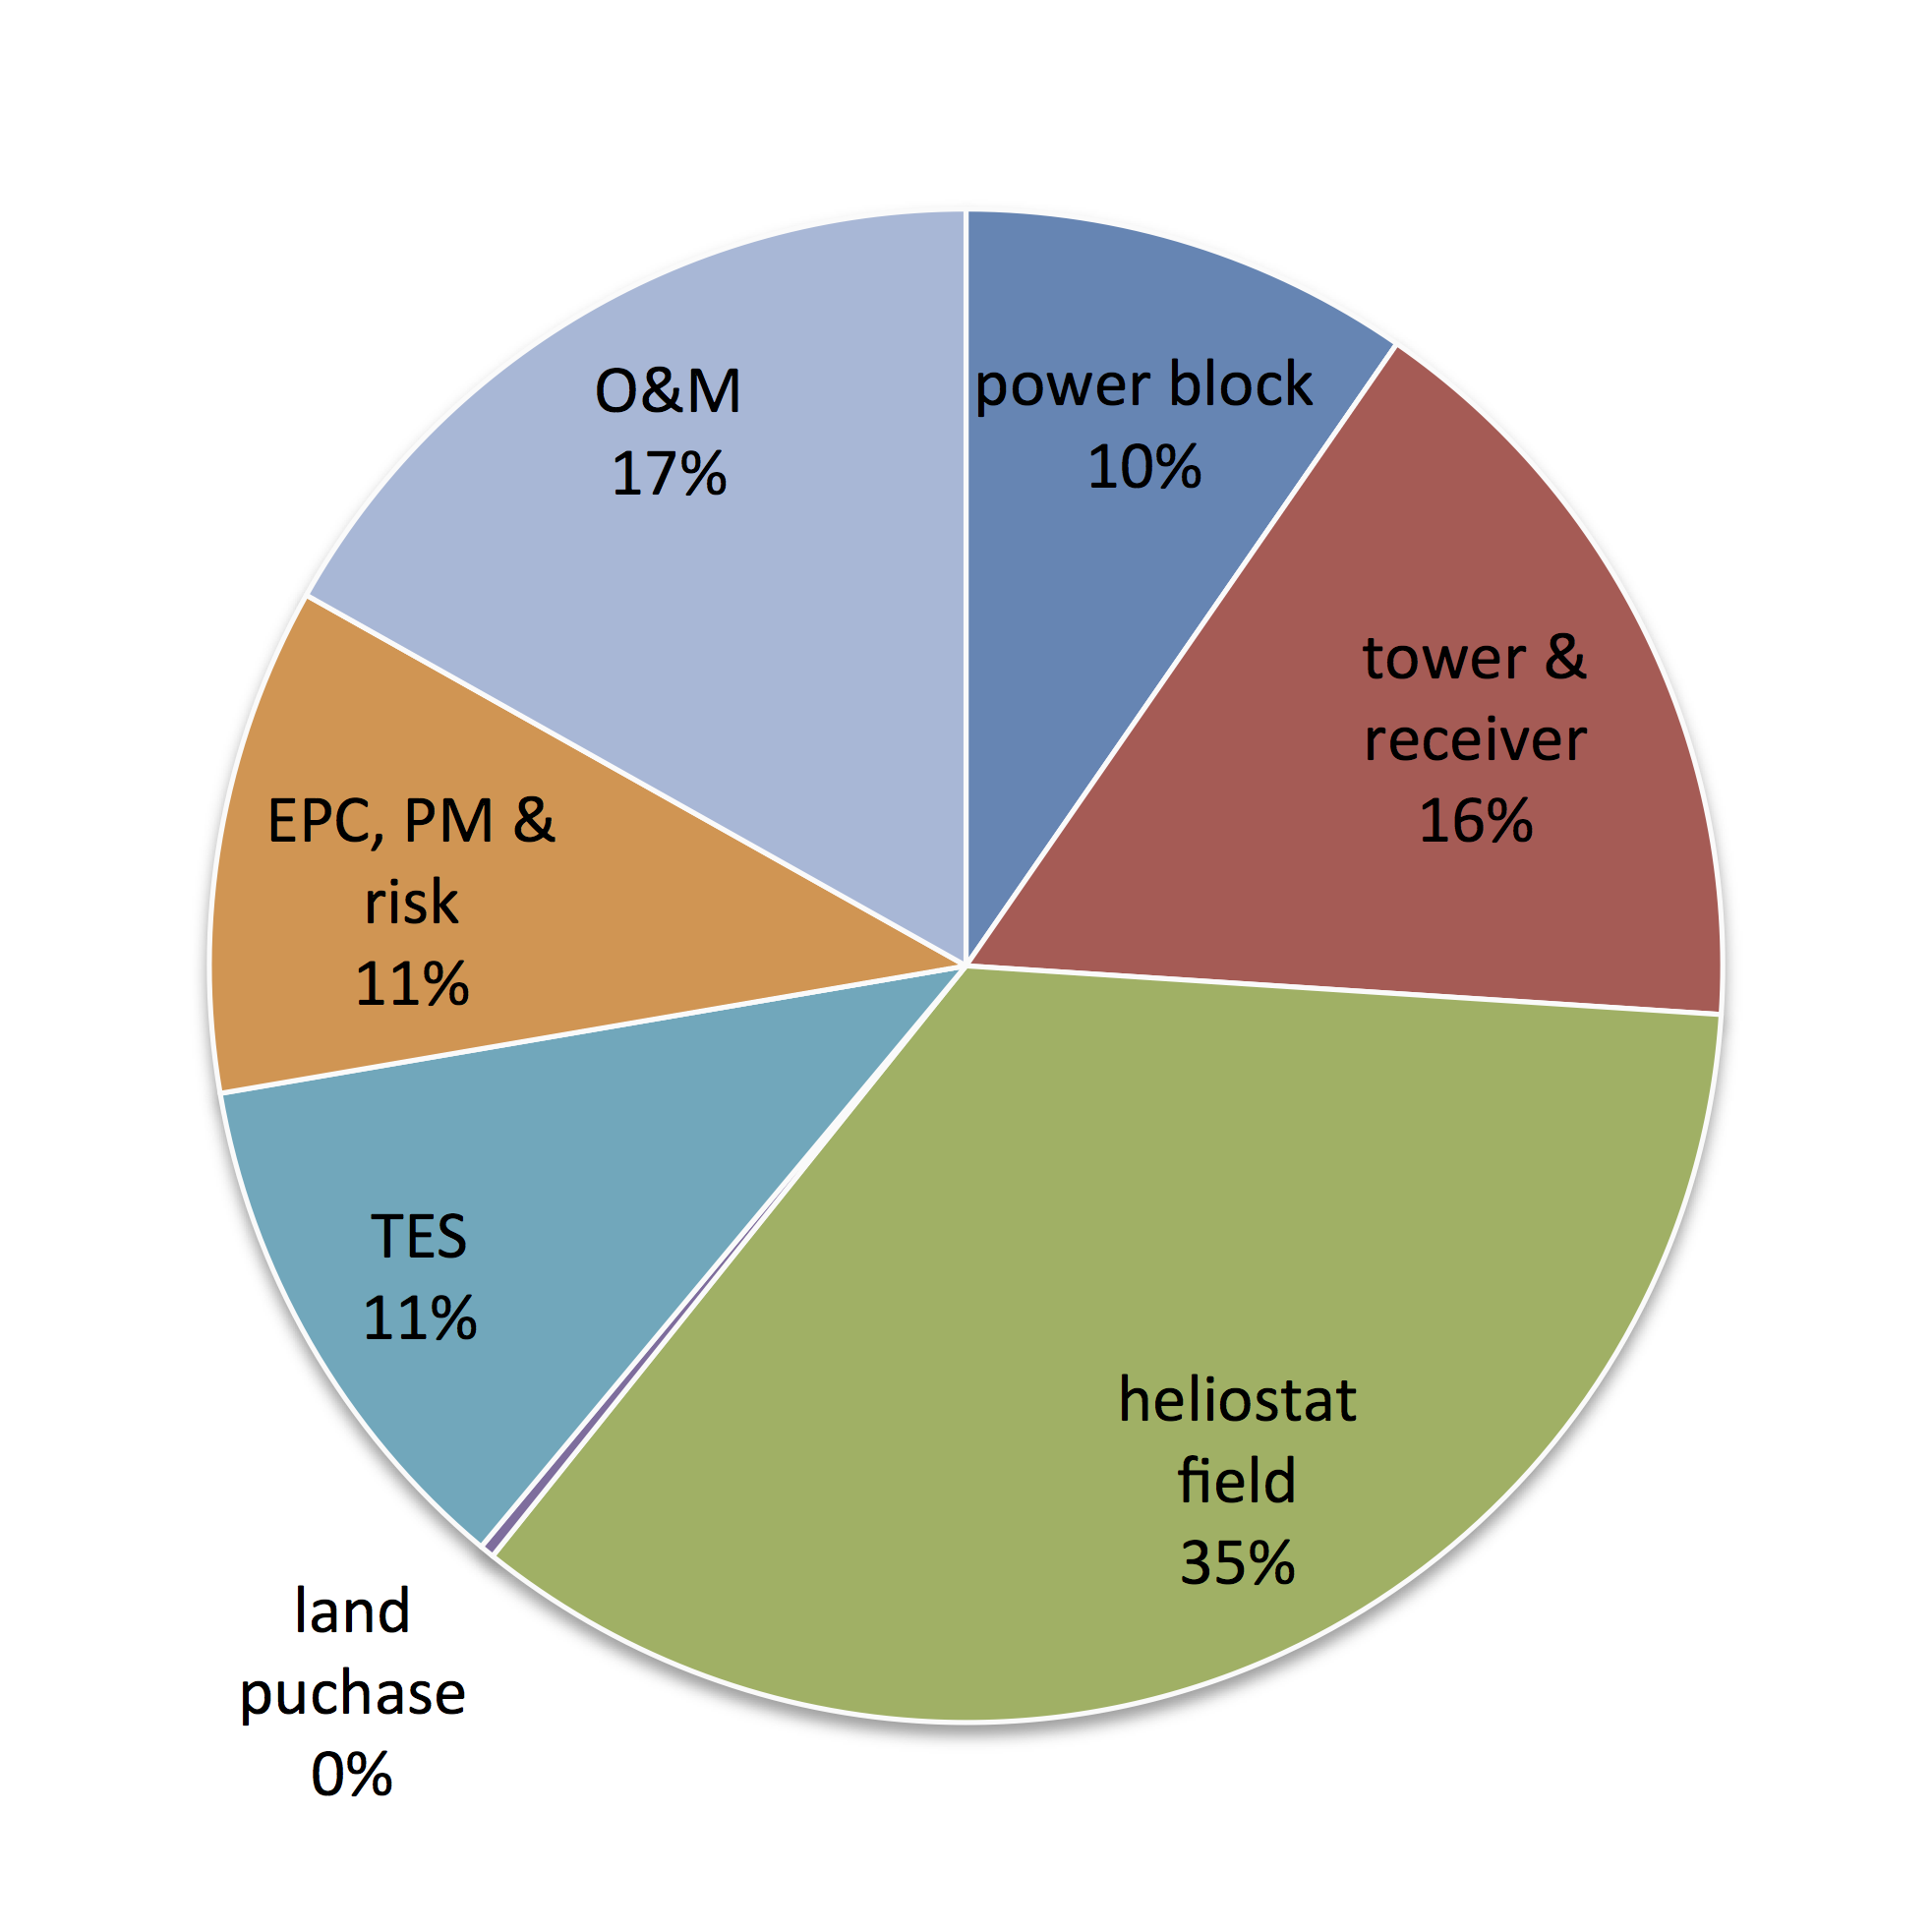
\includegraphics[width=1\textwidth]{FIG/CR_LCOE_highinvest_BreakDown}
                \caption{LCOE break-down for SM~3.5 and \SI{16}{h}~TES.}\label{CR_LCOE_highinvest_BreakDown}
        \end{subfigure}
        \caption[Break-down of selected CR-LCOE calculation results.]{Break-down of selected CR-LCOE calculation results.}\label{CR_LCOE_BreakDown}
\end{figure}
The calculated LCOEs of the simulated CR power plants is composed by seven cost parts. The investment costs of power block, tower and receiver, heliostat field, land purchase, TES, additional EPC, project management (PM) and risk as well as the annual costs for operation and maintain (O\&M). The brake-down of the LCOE components can be seen in Figure~\ref{CR_LCOE_BreakDown} for the simulation of the lowest and the highest configuration.  It can be seen that the investment costs of the land purchase don't have any influence to the LCOE of the simulated CR configurations. Also the share of the EPC, PM and risk as well as the share of O\&M don't varies much.

When comprising the results of the load curve covering with the LCOE calculation the lowest LCOE for reaching the target of 90~\% is the configuration of a SM of 3.0 and \SI{14}{h} of TES. The LCOE for these configuration is \SI{149.58}{USD/MWh}. 

For reaching 80~\% of the prescribed load curve the lowest LCOE is \SI{138.25}{USD/MWh} using a SM of 2.5 and \SI{10}{h} of TES. The lowest LCOE for covering 70~\% of the prescribed load curve is also the lowest LCOE of all and is mentioned above.

\pagebreak
\section{PTC power plant}
\subsection{Design  and simulation} \label{PTC power plant design  and simulation}
The PTC power plant was simulation in the “CSP parabolic trough (physical)" model in SAM using the option "no financial model". As before the input the EPW weather file to specify the hourly atmospheric conditions from Section~\ref{Location and weather data} was used. For the PTC simulation SAM uses the following input data:
\begin{itemize}
\item Latitude ($\,^{\circ}$)
\item Longitude ($\,^{\circ}$)
\item Elevation above sea level (m)
\item DNI (\si{\watt\per\square\metre})
\item Atmospheric pressure (\si{\milli\bar})
\item Dry bulb temperature (\si{\celsius})
\item Wetbulbtemperature(\si{\celsius})
\item Relative humidity (\si{\percent})
\item Wind velocity (\si{\metre\per\second})
\end{itemize}
This Chapter describes in detail the input data of the PTC power plant simulation by there components, namely the  power cycle, solar collector, solar receiver, solar field and thermal energy storage (TES).

Also for the simulation of the PTC are the financial parameters and the LCOE calculated separately Microfoft Excel using a simplified method which is documented in Appendix~\ref{ChapterLCOE} on Page \pageref{ChapterLCOE}.
\subsubsection{Simulated configurations}
In order to reaching the goal of covering 90 \% of the scheduled production curve also the simulated PTC power plant used a variation of solar multiple and full load hours of TES. To covering the scheduled load the solar multiple was varied from 2 to 5.0 in steps of 5.0. This is significantly higher SM compared the simulated CR system was necessary to reach the \SI{90}{\percent} covering factor. As before with the simulation of the CR, the storage full load hours were varied from \si{8} to \SI{16}{h} in steps of \SI{2}{h}. The target of \SI{100}{MW} net capacity was reached with a gross capacity of \SI{120}{MW} with an estimated gross-to-net conversion factor of \si{0.83}. The comparatively high gross turbine output is nessasary for the high parasitic burden of the system. Table~\ref{tbl: PTC_OverallConfig} summarizes the simulated configurations.
\begin{table}[!h]  
  \centering
	\begin{tabular}{ p{4.0cm}  C{1.0cm}  C{0.3cm} C{0.3cm} C{0.3cm} C{0.3cm} C{0.3cm} |C{0.3cm}  C{0.3cm} C{0.3cm} C{0.3cm} C{0.3cm} } 
	\hline	
\textbf{Item} & \textbf{Unit} & \multicolumn{10}{c}{\textbf{Value}} \\ \hline \hline
Net turbine capacity & \si{\mega\wattel} & \multicolumn{10}{c}{100} \\
Gross turbine capacity & \si{\mega\wattel} & \multicolumn{10}{c}{120} \\ \hline
Solar multiple & - & \multicolumn{5}{c}{2.0} & \multicolumn{5}{c}{2.5} \\
TES capacity & h & 8 & 10 & 12 & 14 & 16 & 8 & 10 & 12 & 14 & 16 \\ \hline 
Solar multiple & - & \multicolumn{5}{c}{3.0} & \multicolumn{5}{c}{3.5} \\
TES capacity& h & 8 & 10 & 12 & 14 & 16 & 8 & 10 & 12 & 14 & 16 \\ \hline 
Solar multiple & - & \multicolumn{5}{c}{4.0} & \multicolumn{5}{c}{4.5} \\
TES capacity& h & 8 & 10 & 12 & 14 & 16 & 8 & 10 & 12 & 14 & 16 \\ \hline 
Solar multiple & - & \multicolumn{5}{c}{5.0} & \multicolumn{5}{c}{ } \\
TES capacity& h & 8 & 10 & 12 & 14 & 16 &  \multicolumn{5}{c}{ } \\ \hline 
\end{tabular}
\caption[Simulated PTC solar multiple and thermal energy storage  configurations.]{Simulated PTC solar multiple and thermal energy storage  configurations.}\label{tbl: PTC_OverallConfig}
\end{table}

\subsubsection{Power cycle}
The PTC system also uses the steam Rankine cycle technology. In the modeled cycle, feedwater is heated in open (mixed stream) feedwater heaters with two intermediate turbine extractions - once for high pressure and once for low pressure, and the steam generation equipment consists of a preheater, boiler, and superheater. The HTF temperature at the field outlet is bound primarily by HTF stability, so maximum HTF temperatures for oil troughs typically range between \SI{370}{\celsius} and \SI{410}{\celsius}. The turbine has a gross capacity of \SI{120}{\mega\wattel}. So the net turbine capacity output at design (nameplate) is \SI{100}{\mega\wattel}. The design inlet temperature of the HTF in the steam generator is 393\si{\celsius} and outlet temperature of 293\si{\celsius} at design point and operates at a pressure of 100 bar.



Table~\ref{tbl: PTCPowerplant} shows the input parameter for the power block design in SAM. Besides the capacity of the turbine and the condecer type, the parameters are coming from \cite{Wagner2011}. It is obviously, that the cycle conversion efficiency of the PTC power plant is lower than that one from the CR power plant. This is trace back to the lower cycle temperatures and the thereby resulting lower steam pressure in the turbine.



The air-cooled condenser was selected here as well, because water is an valuable resource in the region of Upington. The cooling system is designed to covers the stem generator thermal power. 
\begin{table}[!h]  
  \centering
	\begin{tabular}{  p{7.0cm}  C{2.0cm}  C{2.0cm} } 
	\hline	
\textbf{Item} & \textbf{Value} & \textbf{Unit} \\ \hline \hline
Turbine design capacity, gross  & 110 & \si{\mega\wattel} \\ 
Turbine design capacity, net & 100 & \si{\mega\wattel} \\ 
Boiler operating pressure & 100 & bar \\ 
Design inlet temperature & 393 & \si{\celsius} \\ 
Design outlet temperature & 291 & \si{\celsius} \\ 
Cycle conversion efficiency & 37.74 & \% \\ 
Steam generator design thermal power & 318.0 & \si{\mega\wattth}  \\
Power block start-up time & 0.5 & h \\ 
Minimum required start-up temperature & 300 & \si{\celsius} \\
Maximum turbine over design operation & 90 & \\
Condenser type & air-cooled & - \\ 
\hline
\end{tabular}
\caption[PTC power block and condecer input parameter in SAM.]{PTC power block and condecer input parameter in SAM.}\label{tbl: PTCPowerplant}
\end{table}
\subsubsection{Solar collector (SCA)}
For the simulation of the PTC system the Ultimate Trough was selected as solar collector assembly (SCA). This collector is currently not in commercial use, but comparable troughs with similar characteristics are under construction. So the Ultimate Trough can be adopted  without technical modifications and no increase of risk. Figure~\ref{PTC_Ultimate_config} shows the information of the technical input parameter for SAM. These coming directly from a publication of the developer of the Ultimate Trough, Flabeg GmbH and sbp sonne GmbH \cite{Riffelmann2014}. 
\begin{figure}[bhtp]
\centering
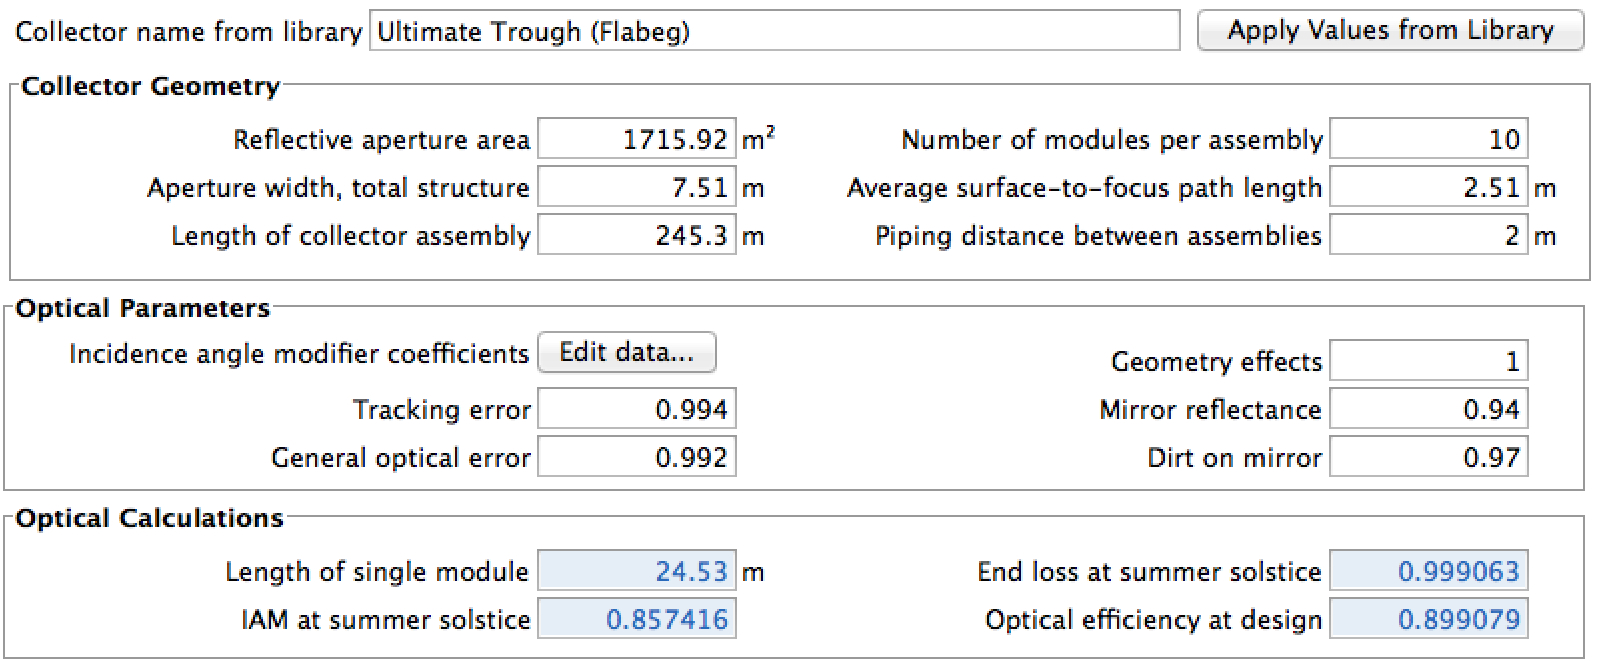
\includegraphics[width=0.95\linewidth]{FIG/PTC_Ultimate_config}
\caption[Screenshot of Ultimate Trough SCA input parameter for SAM.]{Screenshot of Ultimate Trough SCA input parameter for SAM.}\label{PTC_Ultimate_config}
\end{figure}
The section "Optical Calculation" shows, that the total optical efficiency at design of the Ultimate Trough is 89.9~\%. The dimensions and main characteristics of the HCE is shown in the section "Receiver Geometry".
\subsubsection{Solar receiver (HCE)}
As heat collecting element (HCE) Schott's PTR80 was selected. This receiver tube has with \SI{0.08}{m} an extended tube outer diameter. Thereby the tube can contain more HTF and reduce the mass flow in the tubes. Figure~\ref{PTC_HCE} shows the for the simulation inserted parameter. The values are the results of measurements of outdoor optical efficiency and indoor receiver heat loss of parabolic trough collector from researchers of National Renewable Energy Laboratory \cite{Kutscher2012}.
\begin{figure}[htbp]  
\centering
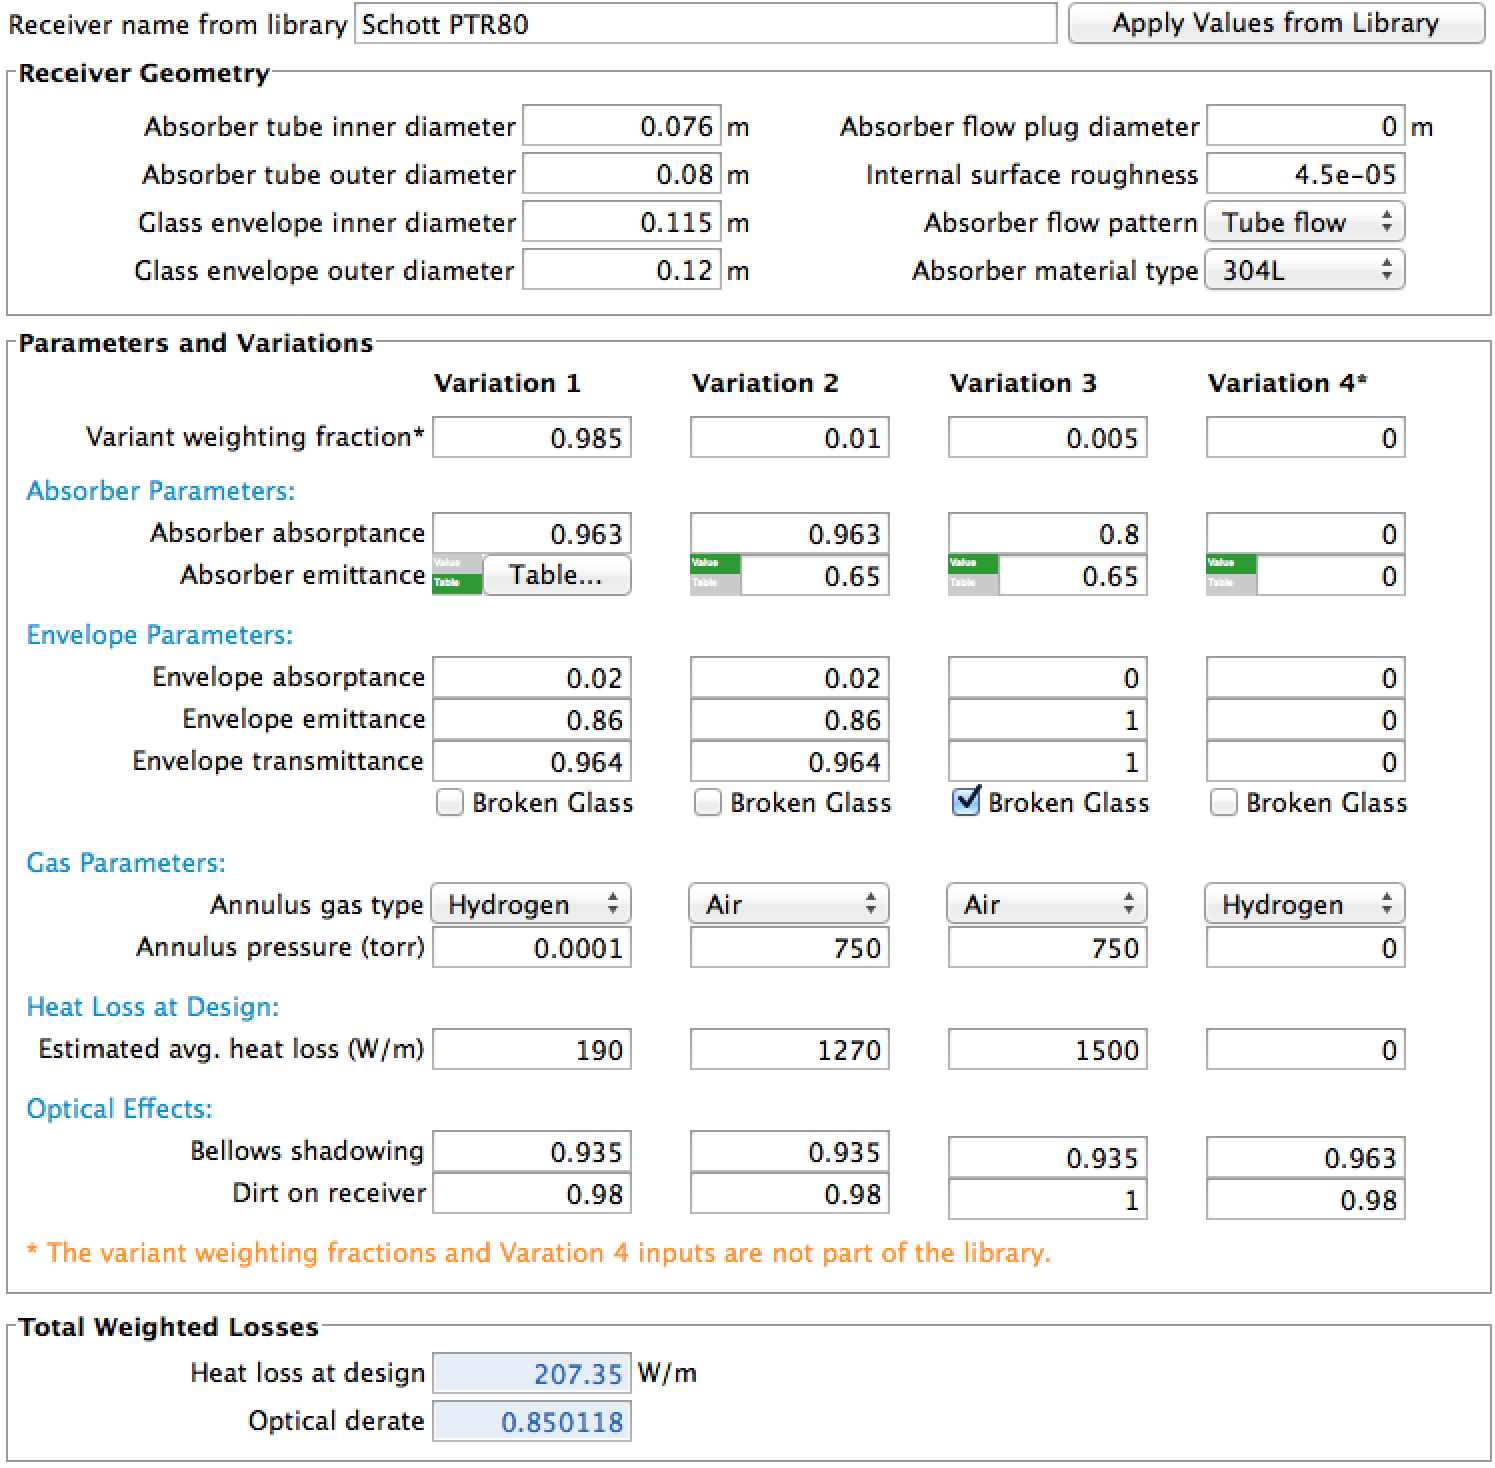
\includegraphics[width=0.95\linewidth]{FIG/PTC_HCE}
\caption[Screenshot of Schott PTR80 input parameter for SAM.]{Screenshot of Schott PTR80 input parameter for SAM.}\label{PTC_HCE}
\end{figure}
The section "Parameter and Variations" shows the different conditions of the HCE. Variation 1 shows the optimal condition of the HCE with annulus pressure of 0.0001 torr (\SI{0.000133}{hPa}), so an vacuum. The estimated average heat lost is \SI{190}{W/m}. This Variation counts for 98.5~\% of all HCEs. In Variation 2 the vacuum is lost and which strongly affects the heat loss. It is 1~\SI{270}{W/m} and counts for 1~\% of all HCEs. In Variation 3 also the protection glass is broken, so the heat loss increase to 1~\SI{500}{W/m}. The total weighted losses is \SI{207.35}{W/m} heat loss at design and about 0.85 optical derate and is shown at the last section most below.
\subsubsection{Solar field}
PTC solar fields are separated in sections. In the simulation of the PTC system the solar field is designed in two sections. Each section carries a feed pipe and a return pipe to transport the thermal energy to the power block. Attached to the header pipes are many loops, which contains the SCAs, the HCEs and the HTF. Figure~\ref{PTC_Field_ultimate} shows an typical layout for PTC system with two field subsections. As in the Figure is the simulated PTC system designed by four SCAs per loop \cite{Riffelmann2014}.
\begin{figure}[htbp]  
\centering
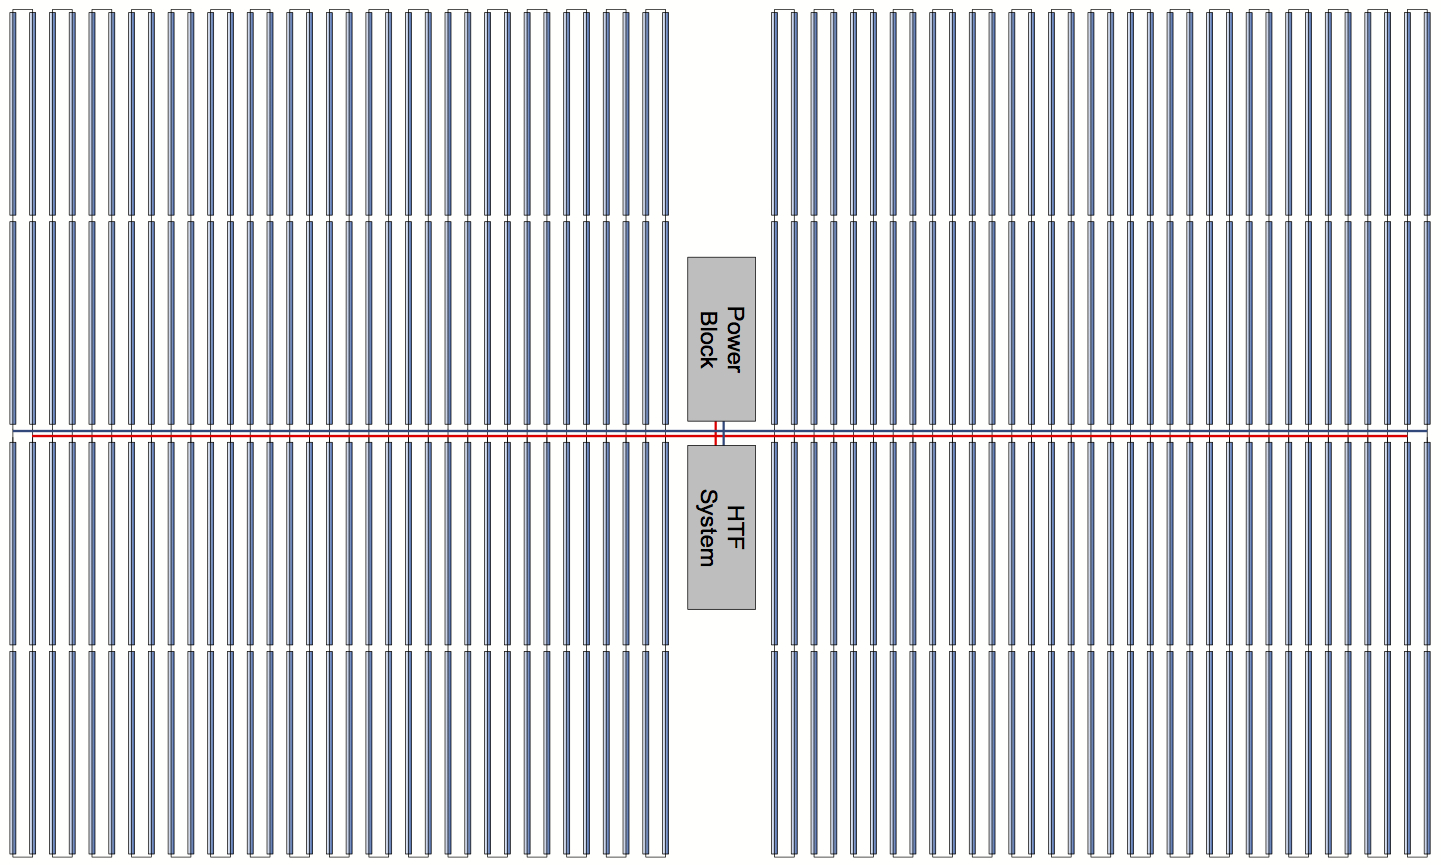
\includegraphics[width=0.9\linewidth]{FIG/PTC_Field_ultimate}
\caption[Typical configuration of a solar field layout with two field subsections for a Ultimate Trough.]{Typical configuration of a solar field layout with two field subsections for a Ultimate Trough \cite{Riffelmann2014}.}\label{PTC_Field_ultimate}
\end{figure}


As mentioned before synthetic oil is used as HTF for the simulation of the PTC system. The current standard for HTF in PTC systems is Terminol VP-1. The input parameter for the HTF are shown in Figure~\ref{PTC_HTF} and are limited by the performance characteristics of Terminol VP-1 of 12 to 400\si{\celsius} \cite{Therminol2015}. The velocity range of Therminol VP-1 should be in the range of 0.36 and 4.97 m/s \cite{Wagner2014} and is affected by the inner tube diameter of the HCE, the HTF density and the loop flow rate \cite{NREL2015a}. A freeze protection temperature for the HTF of 150\si{\celsius} is typically and also assumed for the simulation \cite{Kearney2002}.
\begin{figure}[htbp]  
\centering
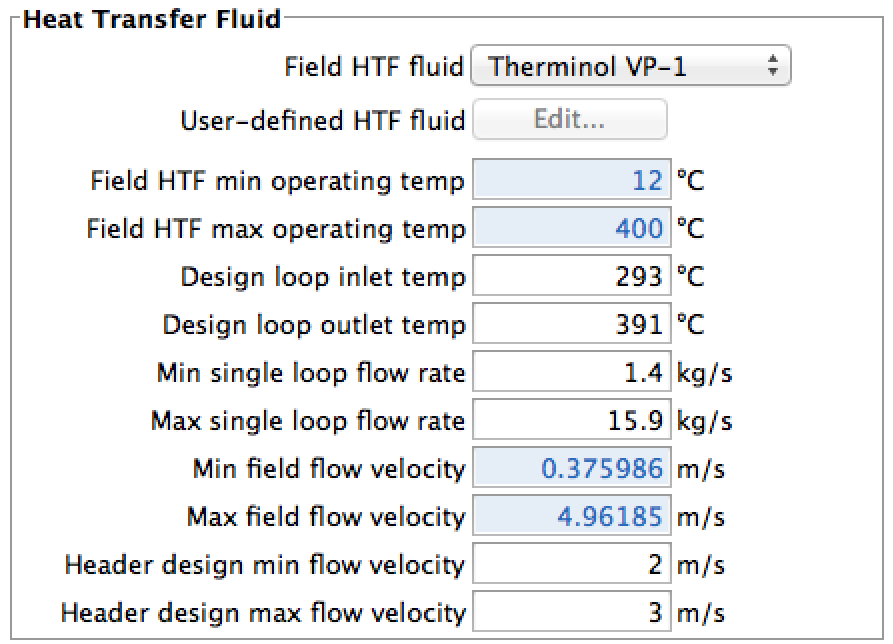
\includegraphics[width=0.6\linewidth]{FIG/PTC_HTF}
\caption[Screenshot of HTF input parameter for SAM.]{Screenshot of HTF input parameter for SAM.}\label{PTC_HTF}
\end{figure}


The size of the solar field is strongly effected by the solar multiple and the thermal demand of the steam Rankine cycle. At a solar multiple of \si{1} (design thermal power of the steam generator) the solar field requires \SI{453003}{\square\metre} ($\approx$\SI{45.3}{ha}) reflective aperture area of SCA. \si{65.86} ($\approx$66) loops are required at a SM of \si{1}. The number of loops and so also the field size multiplies by the value of the SM.



Also the the solar field area and thereby the total land area depending by the SM. Equation~\ref{GL_PTCSolarfieldarea} shows the influence on the solar field area of the ratio between the row spacing and the SCA width. The roe spacing is assumed by \SI{18}{m} between the parallel SCAs. The total land area results by Equation~\ref{GL_PTCtotallandarea} and is the solar field area multiplies by the factor of non-solar field area. The factor is assumed by \si{1.4} in the simulation \cite{NREL2015a}.
\begin{align}
\textrm{solar field area }(m^2) =\textrm{aperture area }(m^2) \times \frac{\textrm{row spacing }(m)}{ \textrm{SCA width }(m)} \label{GL_PTCSolarfieldarea}
\end{align}
\begin{align}
\textrm{total land area }(m^2) =\textrm{solar field area }(m^2) \times  \textrm{non-solar field multiplier}\label{GL_PTCtotallandarea}
\end{align}
Table~\ref{tbl: PTCSolarfield} shows the solar field simulation parameter of the PTC system for the simulation configuration values of the solar multiple. The parameters of the Table comes from the above mentioned relations between the Items. The design power of the steam generator (SG) stays at \SI{318.0}{\mega\wattth} while the solar field thermal output rises proportional through the SM. 
\begin{table}[!h]  
  \centering
	\begin{tabular}{ p{3.3cm} C{1.1cm} C{1.1cm} C{1.1cm} C{1.1cm} C{1.1cm} C{1.1cm} C{1.1cm} C{1.1cm} } 
	\hline	
\textbf{Item} & \textbf{Unit} & \multicolumn{7}{c}{\textbf{Value}} \\ \hline \hline
SG Design power & \si{\mega\wattth} &  \multicolumn{7}{c}{318.0}\\
Design-point DNI & \si{\watt\per\metre} &  \multicolumn{7}{c}{950}\\
\hline
\textbf{Solar multiple} &  & \textbf{2.0} & \textbf{2.5} & \textbf{3.0} & \textbf{3.5} & \textbf{4.0} & \textbf{4.5} & \textbf{5.0}\\ \hline 
Field th. output & \si{\mega\wattth} & 636 & 795 & 954 & 1~113 & 1~272 & 1~431 & 1~590\\
Number of loops  & - & 132 & 165 & 198 & 231 & 264 & 297 & 330\\ 
Aperture refl. area & ha & 90.6 & 113.3 & 135.9 & 158.6 & 181.2 & 203.9 & 226.5\\ 
Total land area & ha & 675 & 845 & 1013 & 1~182 & 1~351 &1~540 & 1~689\\ 
\hline
\end{tabular}
\caption[PTC solar field parameter.]{PTC solar field parameter.}\label{tbl: PTCSolarfield}
\end{table}
\pagebreak
\subsubsection{Thermal energy storage (TES)}
The thermal energy storage (TES) of the simulated PTC system uses a indirect two-tank molten salt system with "Hitec Solar Salt" as storage fluid. This storage fluid is made from sodium nitrate (60~\% NaNO\textsubscript{3}) and potassium nitrate (40~\% KNO\textsubscript{3}). Solar Salt needs an minimum operating temperature of 238\si{\celsius} and and has a maximum operating temperature of 593\si{\celsius}. \cite{Suite2011,Kearney2003}

\begin{table}[htbp]  
  \centering
	\begin{tabular}{ p{3.9cm}  C{1.0cm} C{1.2cm} C{1.2cm} C{1.2cm} C{1.2cm} C{1.2cm} } 
	\hline	
\textbf{Item} & \textbf{Unit} & \multicolumn{5}{c}{\textbf{Value}} \\ \hline \hline
Storage type & - &  \multicolumn{5}{c}{indirect two-tank molten salt}\\
Storage fluid & - &  \multicolumn{5}{c}{Hitec Solar Salt}\\
Hot tank design temp. & \si{\celsius} & \multicolumn{5}{c}{391}\\
Cold tank design temp. & \si{\celsius} & \multicolumn{5}{c}{293}\\
\hline
\textbf{TES full load hours} & \textbf{h} & \textbf{8} & \textbf{10} & \textbf{12} & \textbf{14} & \textbf{16}\\ \hline 
Thermal capacity & \si{\mega\wattth\hour}  & 2~544 & 3~180 & 3~816 & 4~452 & 5~087 \\
Storage volume  & \si{\cubed\metre} & 34~407 & 43008 & 51~610 & 60~212 & 68~813\\
\hline
\end{tabular}
\caption[PTC system TES parameter.]{PTC system TES parameter.}\label{tbl: PTCTES}
\end{table}

The storage design temperatures depends from the solar field design temperatures, so the designed temperature difference is \SI{98}{K}. As it is shown in Table~\ref{tbl: PTCTES} the operating temperature limits fits with the storage tank design temperatures. The heater set point is 265\si{\celsius} for both storage tanks. The TES full load hours goes from 8 to 16 in steps of 2. The thermal capacity and also the storage volume rises with the TES full load hours. The simulated stored thermal capacity reaches from 2~\SI{544}{MWh}\textsubscript{th}  at 8 full load hours up to 5~\SI{087}{MWh}\textsubscript{th} at 16 full load hours. It is obviously, that the storage volume of the PTC needs to be more than 3 times that much than the storage volume of the CR system. This is the result of lower temperature difference of the HTF and the turbine design capacity.

Also for the simulation of the PTC system the dispatch control of the turbine output fraction in the storage settings was used. Figure~\ref{PTC_turbineoutput} shows the dispatch control matrix for the turbine output fraction.
\begin{figure}[htbp]  
\centering
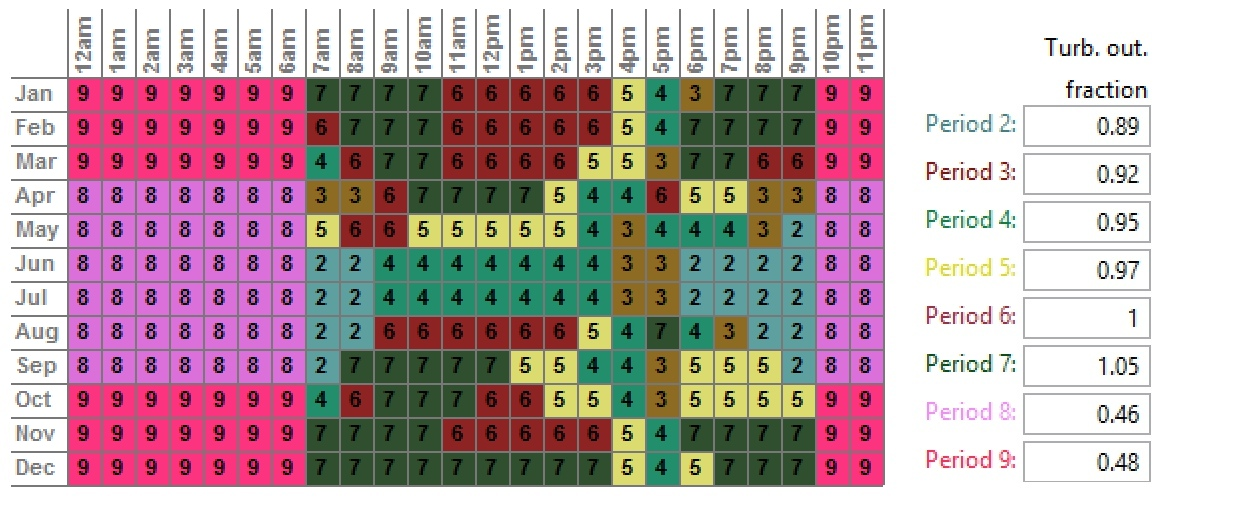
\includegraphics[width=0.95\linewidth]{FIG/PTC_turbineoutput}
\caption[TES dispatch control matrix for turbine output fraction of PTC simulation in SAM.]{TES dispatch control matrix for turbine output fraction of PTC simulation in SAM.}\label{PTC_turbineoutput}
\end{figure}
\subsubsection{Financial parameter}
The financial parameter for calculating the LCOE of the simulated configuration are shown in Table~\ref{tbl: PTCFinance}. As before at the CR is the PTC power plant calculated over a lifetime of \SI{25}{years} using a real interest rate of 7.5~\% \cite{FraunhoferISE2013}. Also the total plant availability of  15~\% once-off surcharge for EPC and contingencies on the total investment costs are equal to the CR \cite{Platzer2014}.


The specific costs for the collector field inclusive HTF-system is assumed with \SI{275}{\usd\per\square\metre} from \cite{Morin2012}. These specific cost could also be reduced by 25~\% by using the assumed cost reduction from Flabeg \cite{FLABEG_FE_GmbH2015}. So the for the simulation assumed costs are highly conservative.

The specific costs for the power block are the same as at the CR but from other sources \cite{Platzer2014}. 

The specific costs of \SI{50}{USD/kWh}\textsubscript{th} for the TES of the PTC are up to 50~\% higher than the CR costs \cite{Platzer2014}. This is reduce to the lower energy density using lower storage temperatures \cite{Steinmann2015}. Other expected specific costs between 35 and \SI{50}{USD/kWh}\textsubscript{th} \cite{Steinmann2012}.

As before Fichtner analyzed also the annual O\&M costs for PTC power plants in SA and results costs of 1.96-1.97~\% of the total investment costs \cite{Fichtner2010}. The value of 2~\% can so also be assumed as conservative.

The costs for the land purchase comes from the "African Agriculture Review" report of the Nedbank Capital, which reported the prices for farmland in SA. For the LCOE calculation of the CSP and PV system was the land purchase costs of 3~\SI{000}{USD/ha} assumed which is based on these report \cite{Cassell2012}.
\begin{table}[!h]  
  \centering
	\begin{tabular}{  p{5.0cm} C{2.0cm} C{1.5cm}  C{1.5cm}  C{4.0cm} } 
	\hline	
\textbf{Item} & \textbf{Symbol}& \textbf{Value} & \textbf{Unit} & \textbf{Source}\\ \hline \hline
Collector field/HTF-system & $c_{CF}$ & 275 & \si{\usd\per\square\metre} & \cite{Morin2012}\\ 
Power block &$c_{PB,PTC}$ & 1000 & \si{\usd\per\kilo\wattel} & \cite{Platzer2014}\\ 
Thermal energy storage & $c_{TES,PTC}$ & 50 & \si{\usd\per\kilo\wattth\hour} & \cite{Platzer2014}\\ 
Land purchase & $c_{LP}$ & 3~000 & \si{\usd\per\hectare} & \cite{Cassell2012} \\ 
Annual O\&M & $f_{O\&M,PTC}$ & 2 & \si{\percent} &\cite{Fichtner2010}\\ 
\hline
Lifetime&$n$ & 25 & \si{\year} & \cite{FraunhoferISE2013} \\ 
Interest rate& $i_{PTC}$& 7.5 & \si{\percent} & \cite{FraunhoferISE2013} \\ 
Annual insurance costs& $f_{ins,PTC}$ & 0.5 & \si{\percent} & \cite{IRENA2012}\\
Surcharge for EPC, project management and risk & $f_{EPC,PTC}$ & 15 & \si{\percent} & \cite{Platzer2014} \\
Total plant availability &$f_{avail,plant,PTC}$ & 96 & \si{\percent} & \cite{Morin2012} \\ 
\hline
\end{tabular}
\caption[Finacial input parameter for PTC-simulation in SAM.]{Finacial input parameter for PTC-simulation in SAM.}\label{tbl: PTCFinance}
\end{table}
\subsection{Results of PTC power plant simulation} \label{sec.resultsPTC}
This section comprised the results of the simulation from the above designed PTC power plant and there belonging LCOE results. Therefore the load curve covering performance and the belonging load profiles and duration curves are described and analyzed. The goal of these Section is to find the suitable PTC design configuration to reach 90~\% covering of the prescribed load which having the lowest belonging LCOE calculation result.
\subsubsection{Load curve covering}
As it was shown in Table~\ref{tbl: PTC_OverallConfig} on Page~\pageref{tbl: PTC_OverallConfig} the PTC system based power plant was simulated in 35 different configurations, using a SM from 2.0 to 5.0 and 8 to \SI{16}{h} of TES, in order to reach the target of 90~\% load curve covering. This section compares the results of the configuration with the lowest SM and TES hours (SM: 2.0 \& TES: \SI{8}{h}) with the configuration using the highest SM and TES hours  (SM: 5.0 \& TES: \SI{16}{h}) representative for all in between.  

The annual average load curve covering result of the selected simulated PTC configurations is shown in Figure~\ref{PTC_annual_profil}. It can be seen, that the PTC power plant using a SM of 5.0 and \SI{16}{h} of TES covers mostly any time of the year the prescribed load curve. But it is also obviously that power supply declines during the night from \SI{3}{am} on and is also decreasing in the morning hours at \SI{8}{am}. In comparison to that covers the PTC power plant using a SM of 2.0 and \SI{8}{h} of TES significantly less of the year the prescribed load curve. This simulated configuration of the PTC system starts declining the covering directly in the afternoon and standstill during the night from 3 to \SI{6}{am} during the whole year. All annual average load profile simulation results can be found in Appendix~\ref{all_load_profile}.

\begin{figure}[htbp]  
\centering
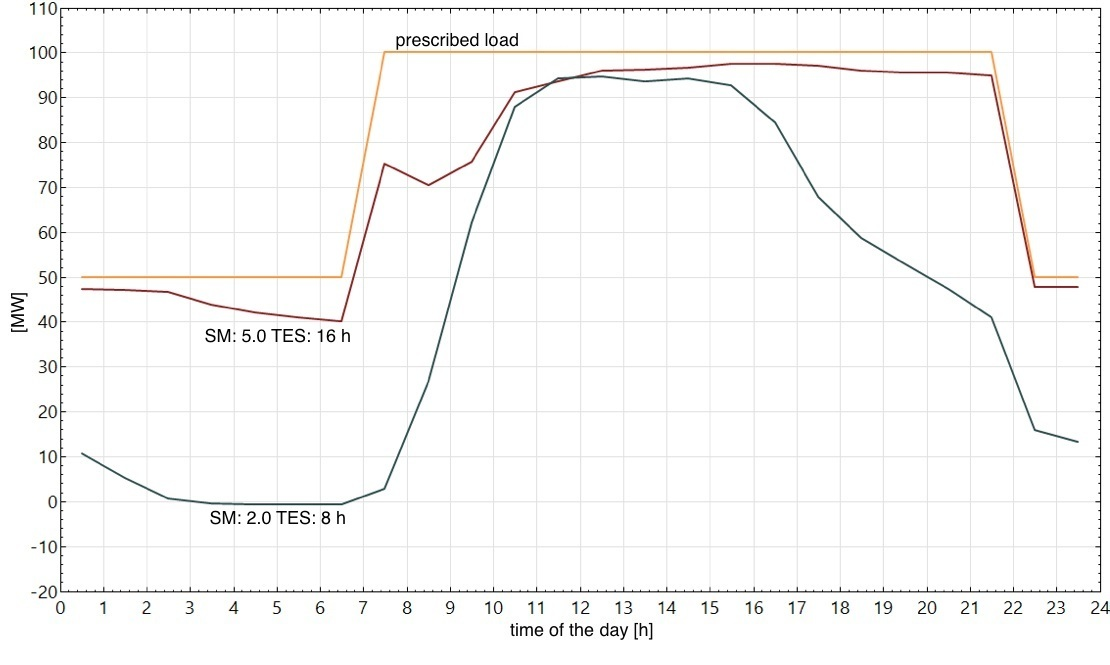
\includegraphics[width=0.8\linewidth]{FIG/PTC_annual_profil}
\caption[Annual average load profile of selected PTC power plant configurations.]{Annual average load profile of selected PTC power plant configurations.}\label{PTC_annual_profil}
\end{figure}
The annual average load curve covering coming from the covering of the prescribed load at any time of the year through the net output of the power plant. The net output variate at any time step and depends on one side from the local whether date and on the other side from the set parameters. The annual sun paths diagram of Upington can be seen on Page~\pageref{SunPathUpington} in Figure~\ref{SunPathUpington}. 

Figure~\ref{PTC_winter_load} shows the load curve behavior of the selected PTC power plant configurations during the time of winter solstice, so the time with the shortest time of sunlight and the lowest angle of the incoming sunlight in Upington, SA. In the portrayed time line the DNI coming fro the whether file has a maximum of a about \SI{830}{\watt\per\square\metre} in peak times and there are also days with lower or almost no direct irradiance. 

The net electricity production of the PTC power plant with low configurations don't reach the prescribed load at any time in this portrayed time line. Therefore it is obviously that the solar field don't collect enough thermal energy during the day for filling up the storage to supply the steam turbines also by night. The power that is produced by the solar field goes at any time directly to the power generation and without direct sun irradiance the production is coming to standstill. The parasitic consumer has a peak load of about \SI{8}{MW} during these days in these configuration.

In comparison to that is reaches the net electricity production of the PTC power plant with high configurations almost everyday the prescribed load for some hours. These configuration can also produce enough thermal energy by the solar field to fill up the storage to produce energy till after midnight. But also in that configuration is coming to standstill every night and rises first with the incoming direct irradiance again. In this configuration there is a peak load of about \SI{12}{MW} coming from the parasitic consumer. 

The overproduction of the net output depends on the gross output control and the variable parasitic consumers. The turbine output was preset for all PTC power plant simulation using the turbine output fraction of the TES dispatch control matrix which illustrated in Figure~\ref{PTC_turbineoutput} on Page~\pageref{PTC_turbineoutput}. So it was not possible to regulate the net output under variable external influences at any time. 

\begin{figure}[htbp]  
\centering
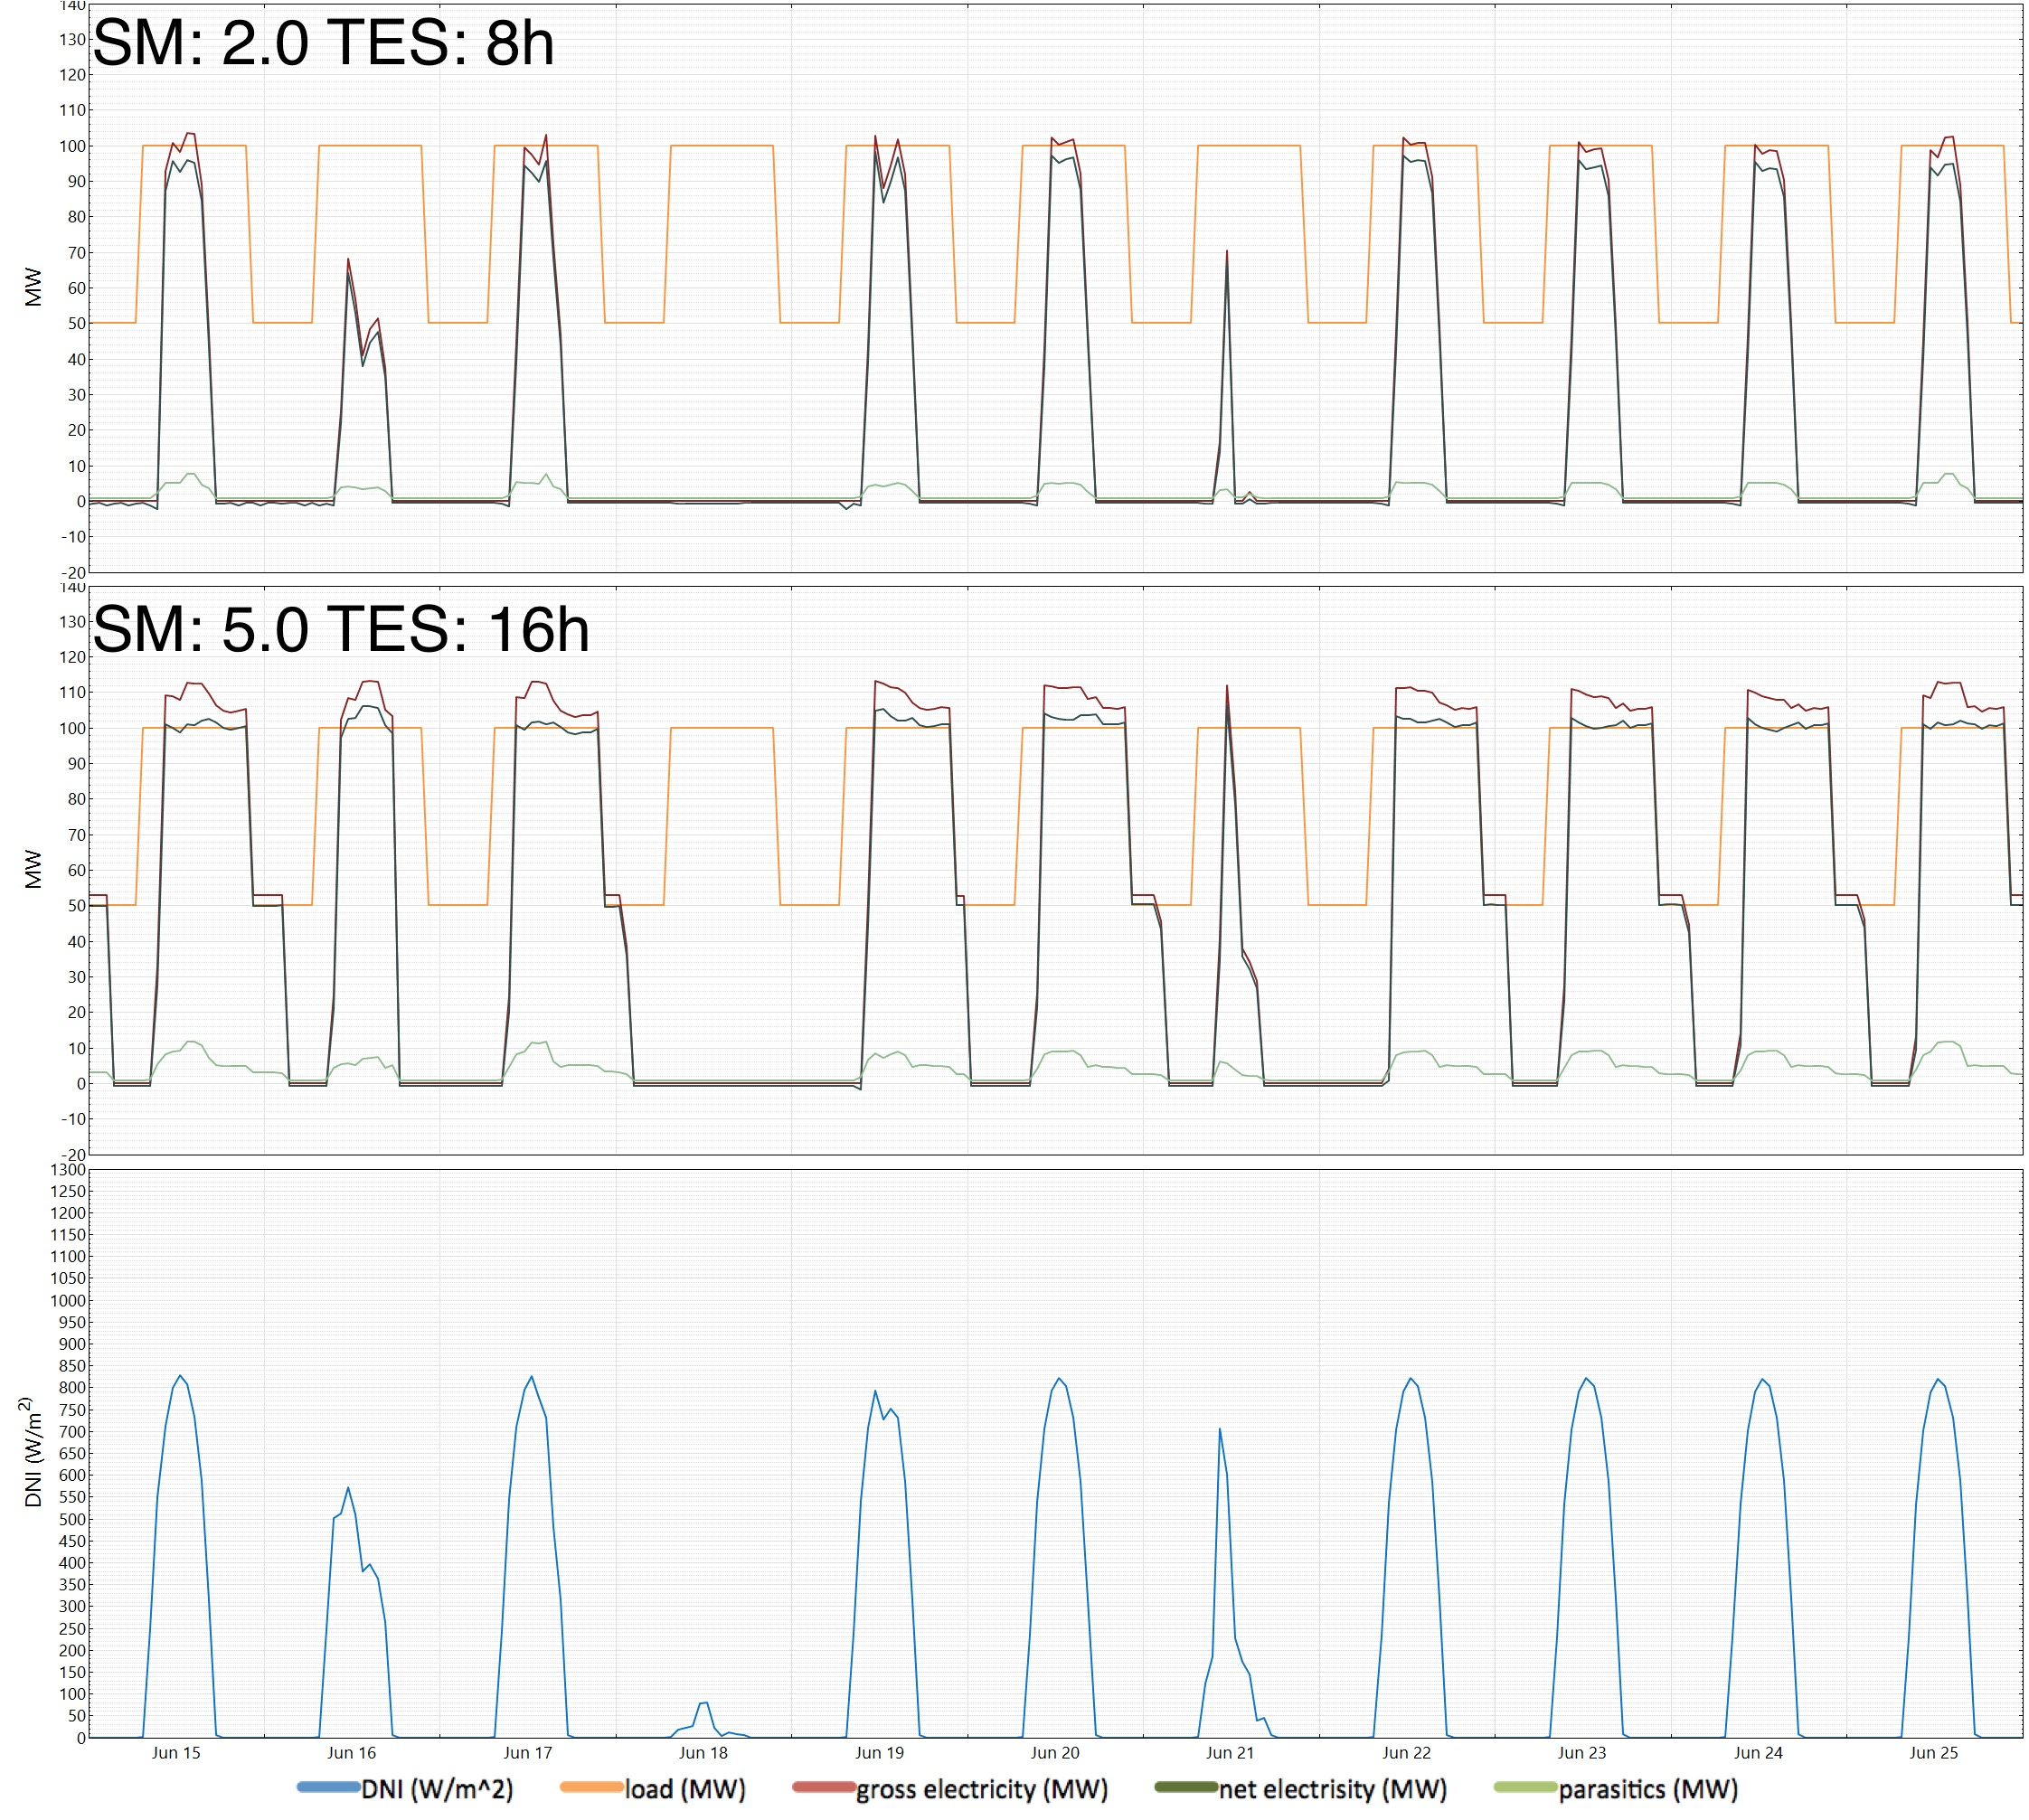
\includegraphics[width=1\linewidth]{FIG/PTC_winter_load}
\caption[PTC load profile during the time of winter solstice (15. June - 25. June).]{PTC load profile during the time of winter solstice (15. June - 25. June).}\label{PTC_winter_load}
\end{figure}
It is obviously that the performance of the PCT power plant isn't great at all during the winter solstice. Neither under high then low performance configurations. This leads mainly from the declining optical performance of the solar collector field under impact of lower sunlight angle during the winter months. This performance loss can mainly reduce to the cosine efficiency of the solar field. Figure~\ref{PTC_field_eff} gives an impression of the strong influence of the cosine efficiency on the total optical field efficiency of the simulated PTC power plants. It can be seen that the cosine effect reduces the total field efficiency by almost 50~\% during the midday in June. 

\begin{figure}[!htbp]
        \centering                
        \begin{subfigure}[b]{0.5\textwidth}
                \centering
                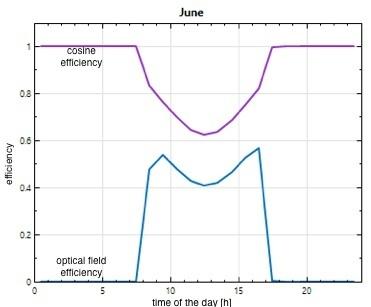
\includegraphics[width=1\textwidth]{FIG/PTC_field_eff_winter}
                \caption{Avarage influence of the cosine efficiency on the avarage total optical field efficiency in June.}\label{PTC_field_eff_winter}
        \end{subfigure}%
        ~
        \begin{subfigure}[b]{0.5\textwidth}
                \centering
                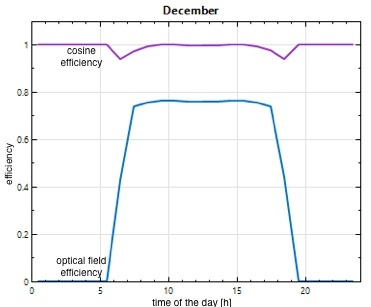
\includegraphics[width=1\textwidth]{FIG/PTC_field_eff_summer}
                \caption{Avarage influence of the cosine efficiency on the avarage total optical field efficiency in December.}\label{PTC_field_eff_summer}
        \end{subfigure}
        \caption[Avarage influence of the cosine efficiency on the avarage total optical field efficiency of a PTC power plant for different months of the year.]{Avarage influence of the cosine efficiency on the avarage total optical field efficiency of a PTC power plant for different months of the year.}\label{PTC_field_eff}
\end{figure}
The loss in optical field performance by the cosine effect arise from the low angle of sunlight, therefor is the efficiency loss in the summer months through the cosine effect comparability low and has just an low effect in the morning and evening hours. 

The load behavior of the two exemplary PTC power plants during the summer solstice is shown in Figure~\ref{PTC_summer_load}. It is obviously that the higher values of the DNI which reaches 1~\SI{150}{\watt\per\square\metre} in peak and the better field efficiency leads to a considerably higher covering of the prescribed load in both configurations. 

The lower PTC configuration which is using a SM of 2.0 and \SI{8}{h} of TES can cover almost the full daytime load and a part of the night time load eith the net electricity production. But under this configuration the PTC power plant can't cover the prescribed load during the night at the best irradiance time of the year, therefrom is also the mentioned gap in production in the annual average load curve coming which was mentioned at the beginning of these section. The net electricity production over-scaled prescribed load at the beginning of the days which leads from the mentioned gross power output control. The parasitic consumers reaching a peak demand of \SI{15}{MW} in this configuration. 

Figure~\ref{PTC_summer_load} shows also the load behavior of the PTC power plant with the highest simulated configuration, which doesn't stand still in this portrayed time span. The graph shows that the net out put is not constant at all. This is coming from the gross power output control and from the massive rises from the parasitic consumers, especially the solar field HTF pump. These pump needs to move a high volume of HTF through the HCEs. At a SM of 5.0 the solar field produce 5 times that much heat then the steam turbine actually needs at the design point. This over-scaling is necessary for the energy production in winter times during the night. Therefore the fractions of focused SCA's getting reduced when the generated energy filled up the storage completely and no more energy in demanded by the steam turbine. This is what  happens to the total parasitic consumption in the chart. The fractions of focused SCA's getting reduced so the power of solar field HTF pump is getting reduced as well. The peak of the parasitic consumers reaching a demand of about \SI{33}{MW} which makes about 27.5~\% of the gross turbine capacity.

\begin{figure}[htbp]  
\centering
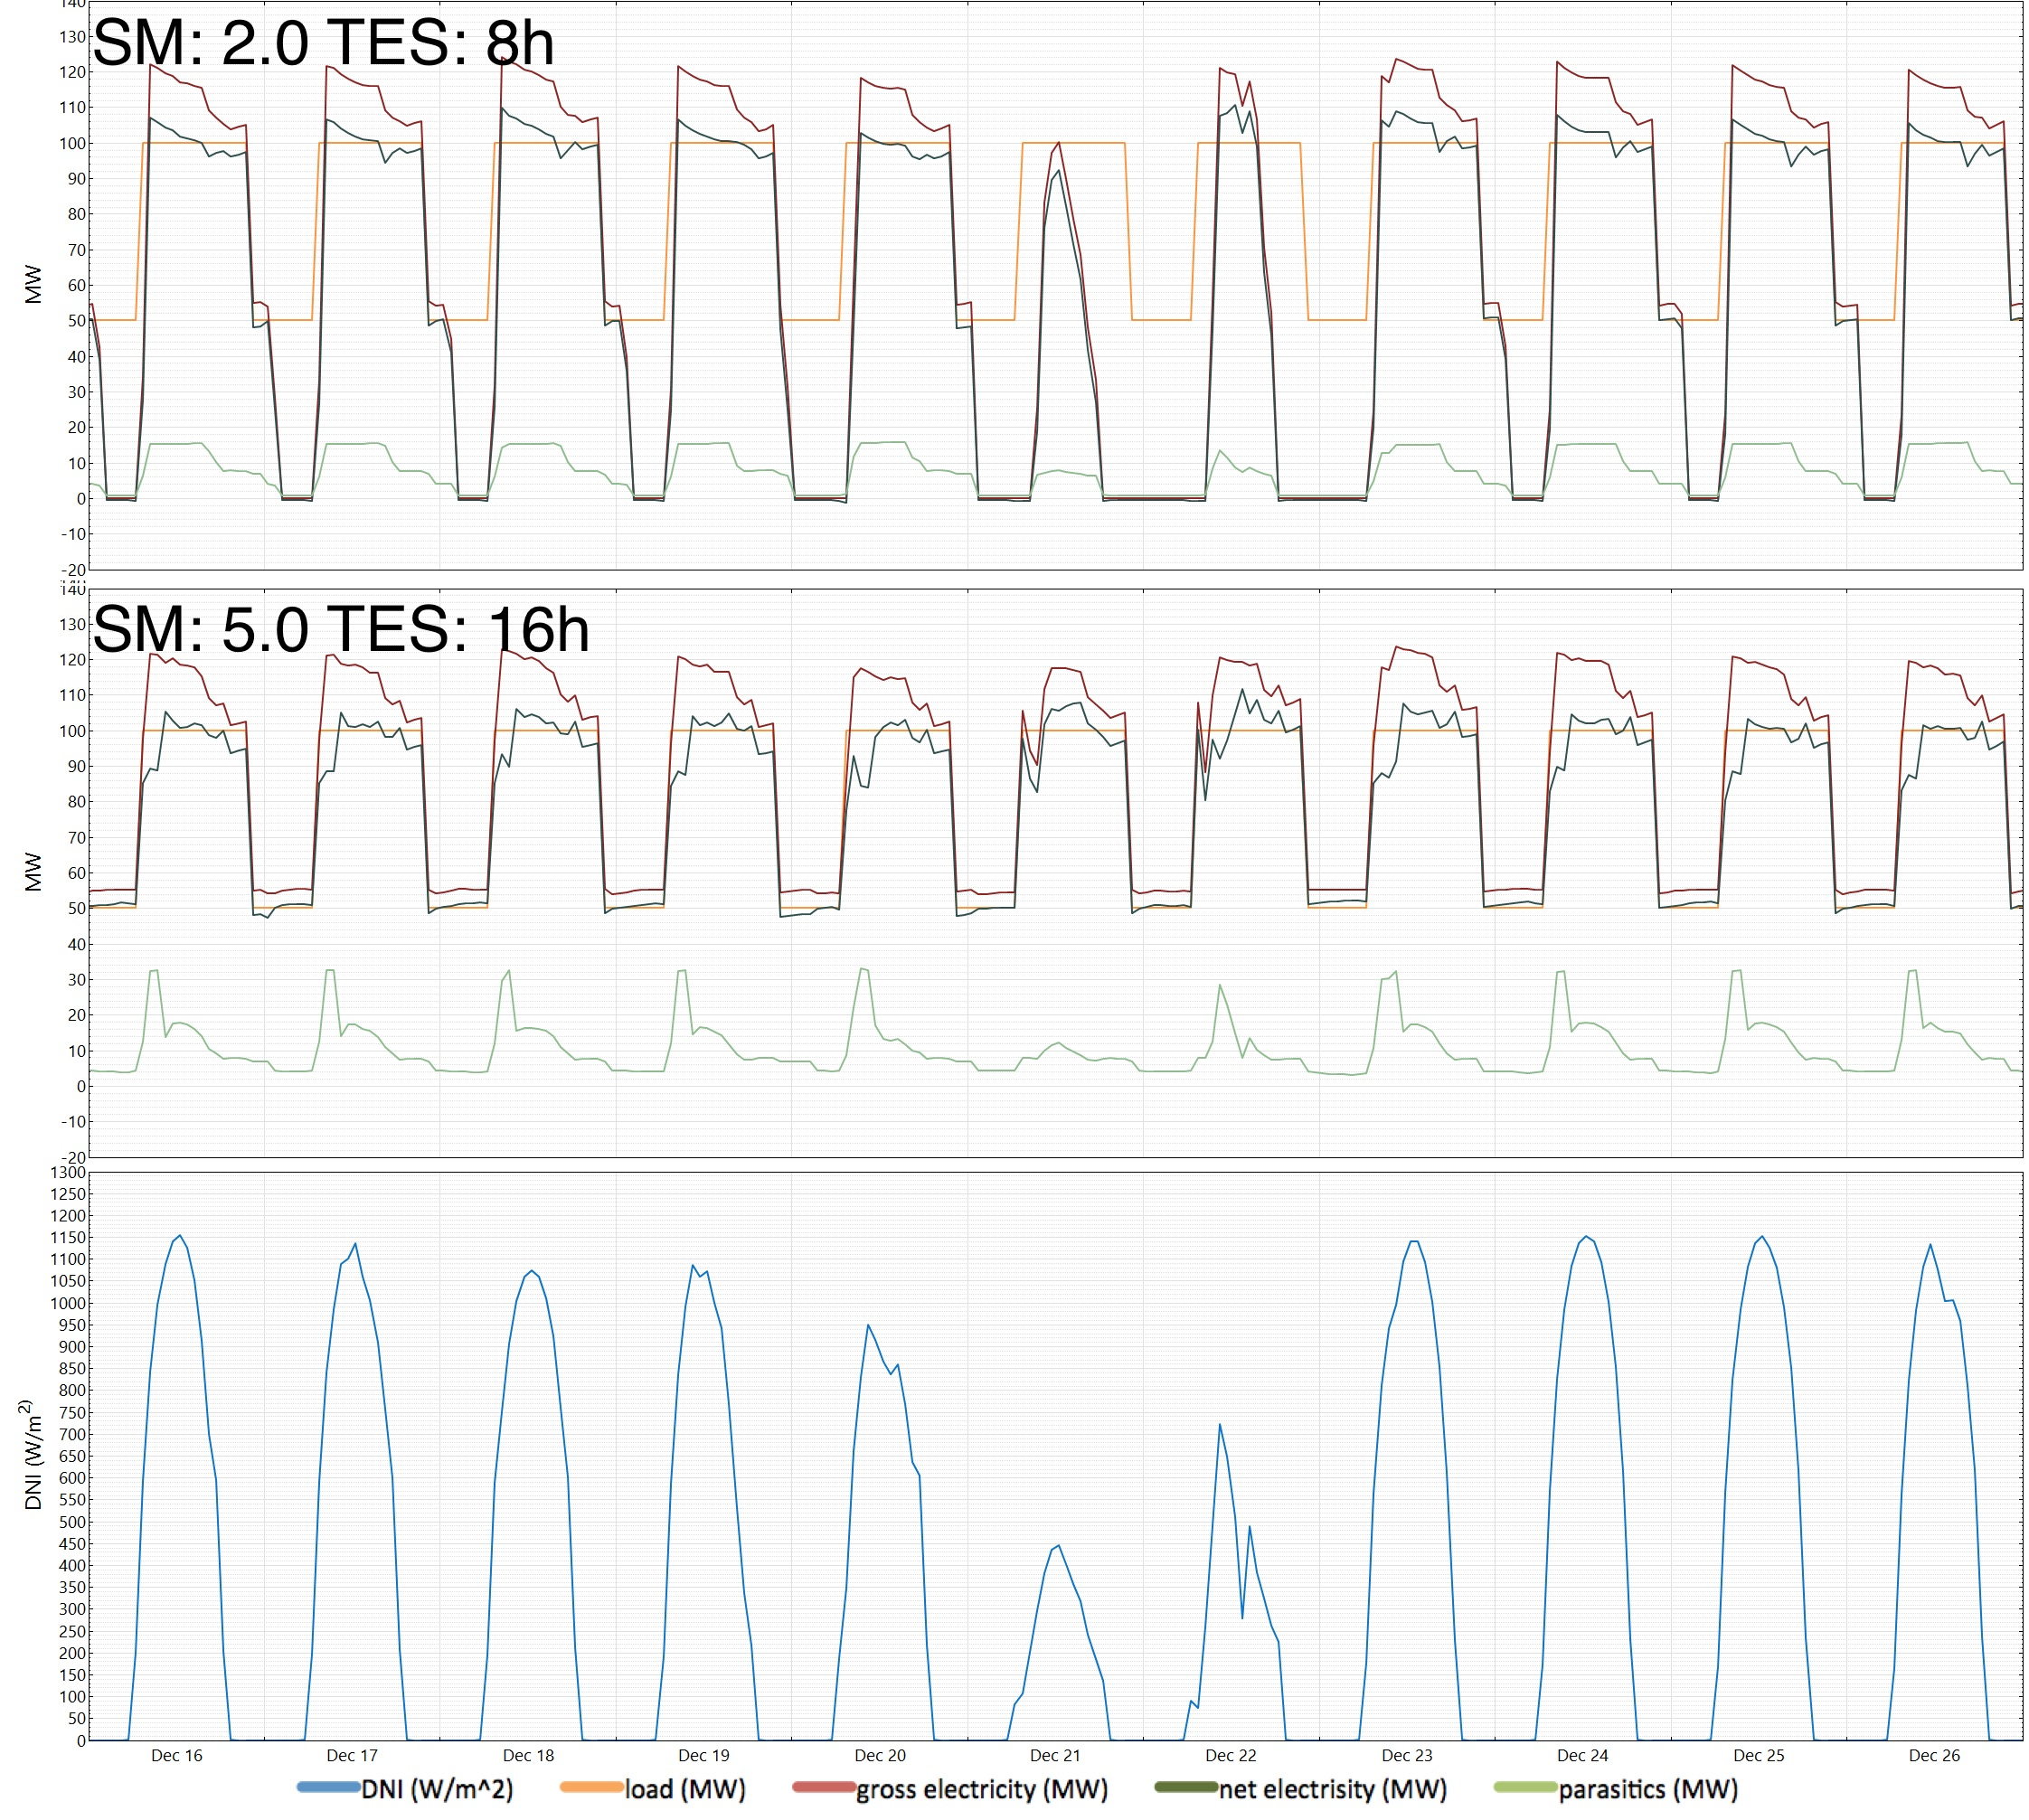
\includegraphics[width=1\linewidth]{FIG/PTC_summer_load}
\caption[PTC load profile during the time of summer solstice (16. December - 26. December).]{PTC load profile during the time of summer solstice (16. December - 26. December).}\label{PTC_summer_load}
\end{figure}
The parasitic demand is composed from different electrical loads of the PTC power plant. Dominantly is the mentioned solar field HTF pump but also the condenser operation of the power cycle. Additionally are the parasitic consumption of the TES \& cycle HTF pump, the field collector drives and the fixed loads. Figure~\ref{PTC_parasitics} shows the share of the produced gross energy of the selected configurations for the simulated year. About 10~\% of the annual gross energy production is going to the parasitic consumers. Therefrom goes about one-third respectively to the condenser operation and the solar field HTF pump. The reaming parasitic load is shared by the TES \& cycle HTF pump and the fixed loads. The share of the field collector drives to the parasitic loads is below 1~\% in any case.

\begin{figure}[!thbp]
        \centering   
        \begin{subfigure}[b]{0.65\textwidth}
                \centering
                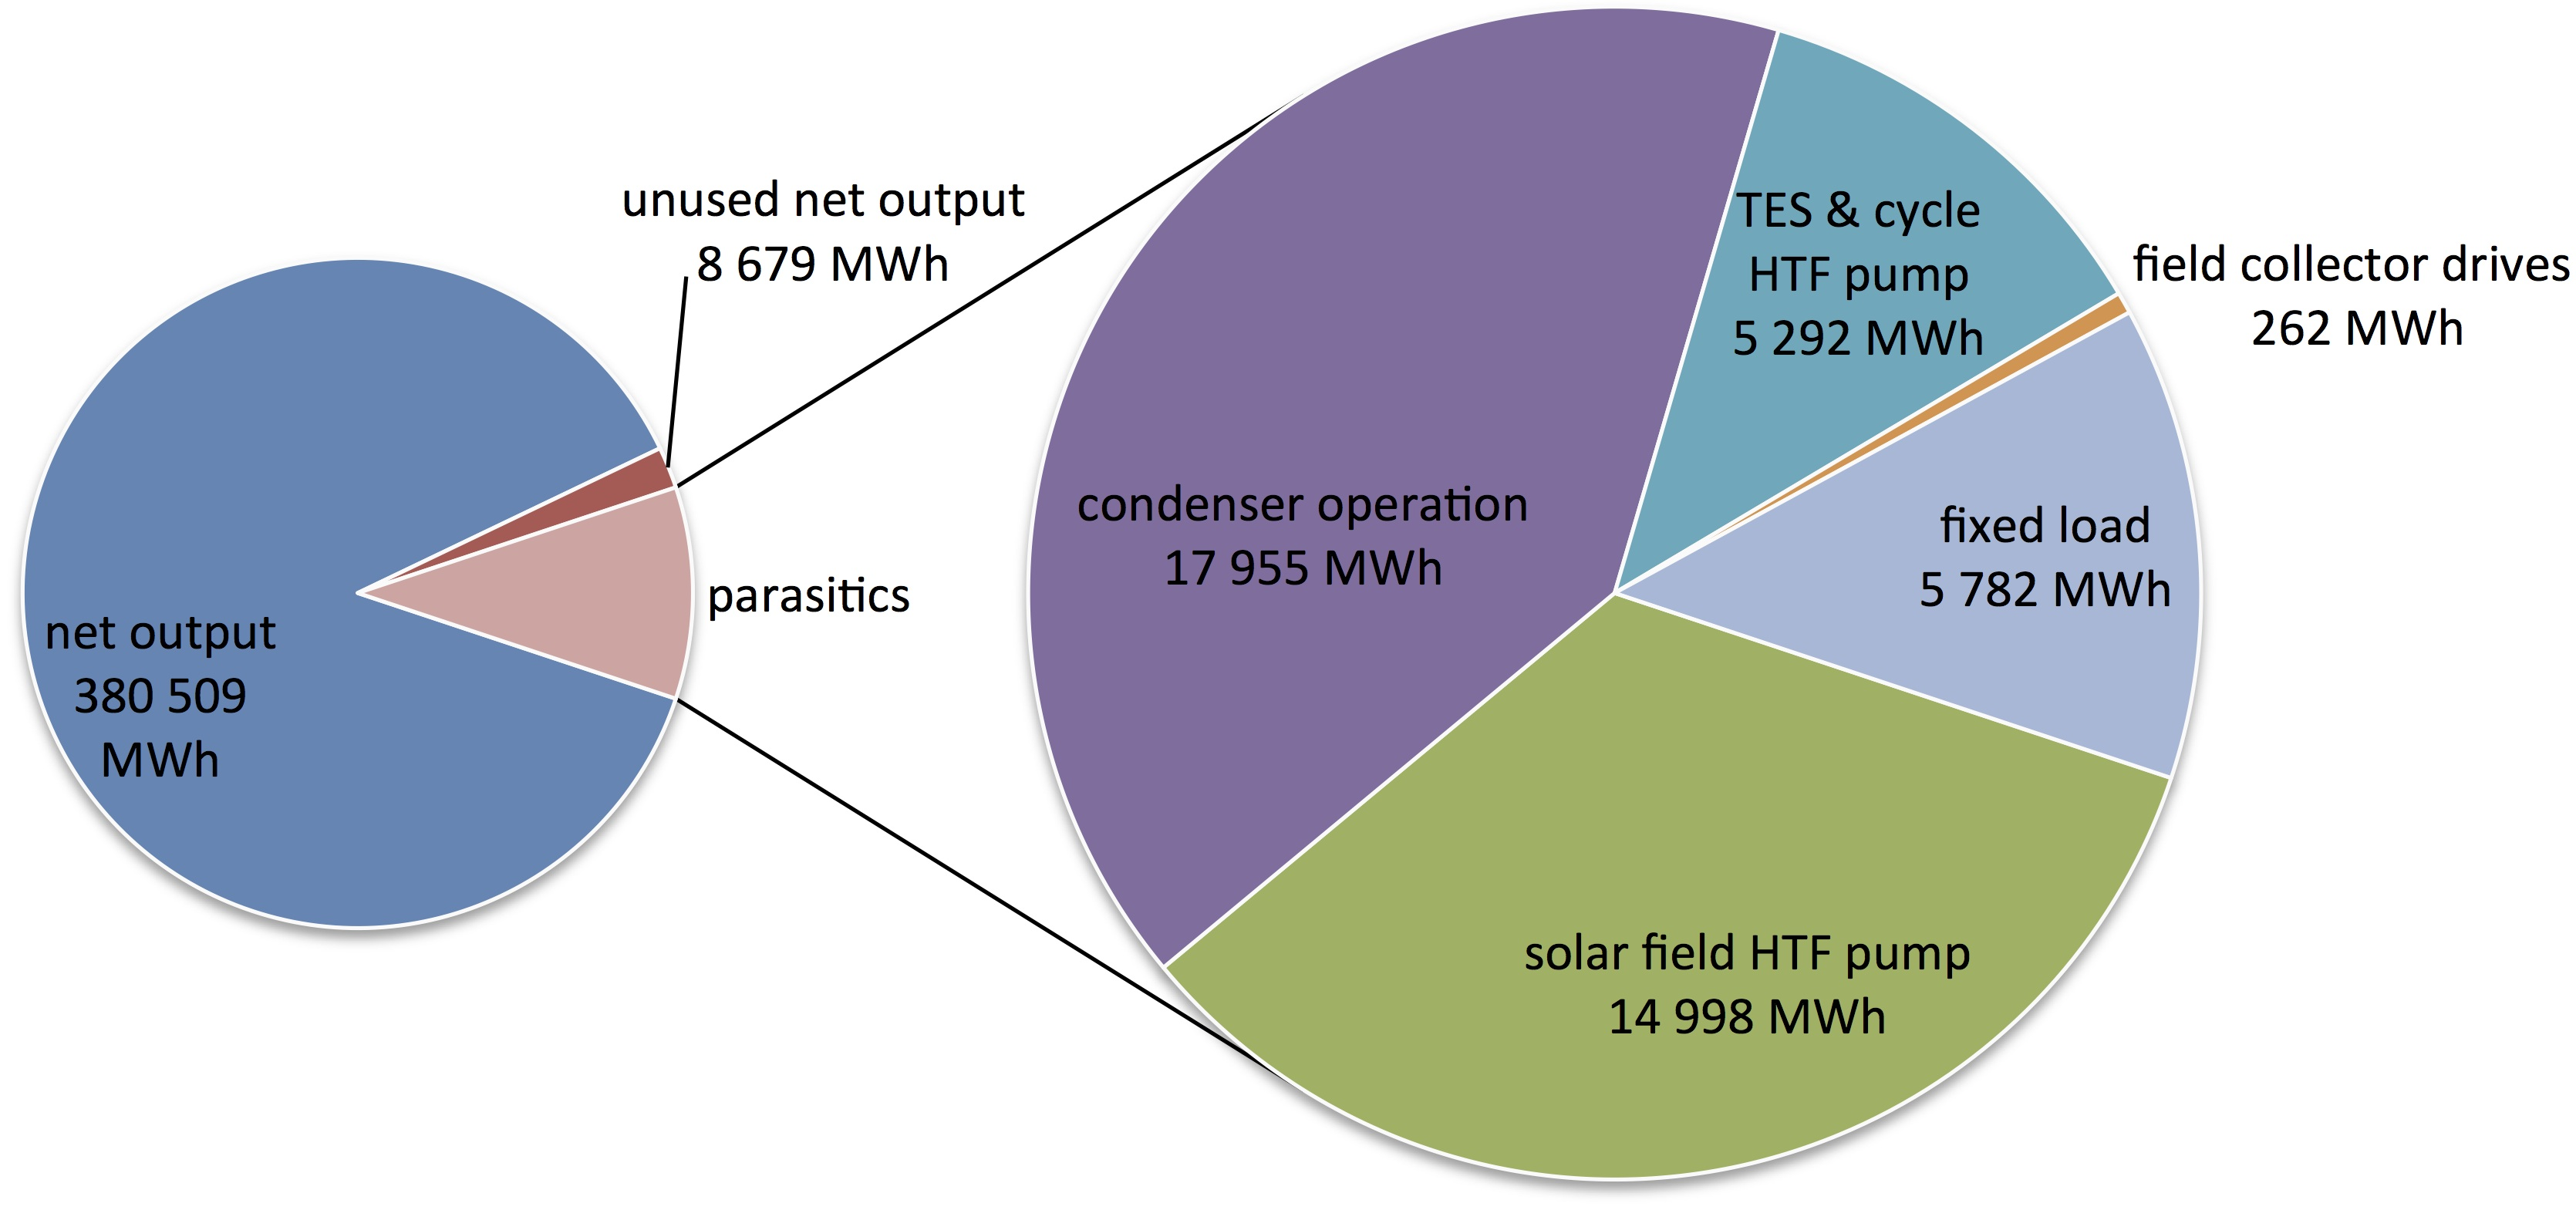
\includegraphics[width=1\textwidth]{FIG/PTC_parasitics_low}
                \caption{SM: 2.0 TES: 8 h}\label{PTC_parasitics_low}
        \end{subfigure}
\par\medskip % Linebreak              
        \begin{subfigure}[b]{0.65\textwidth}
                \centering
                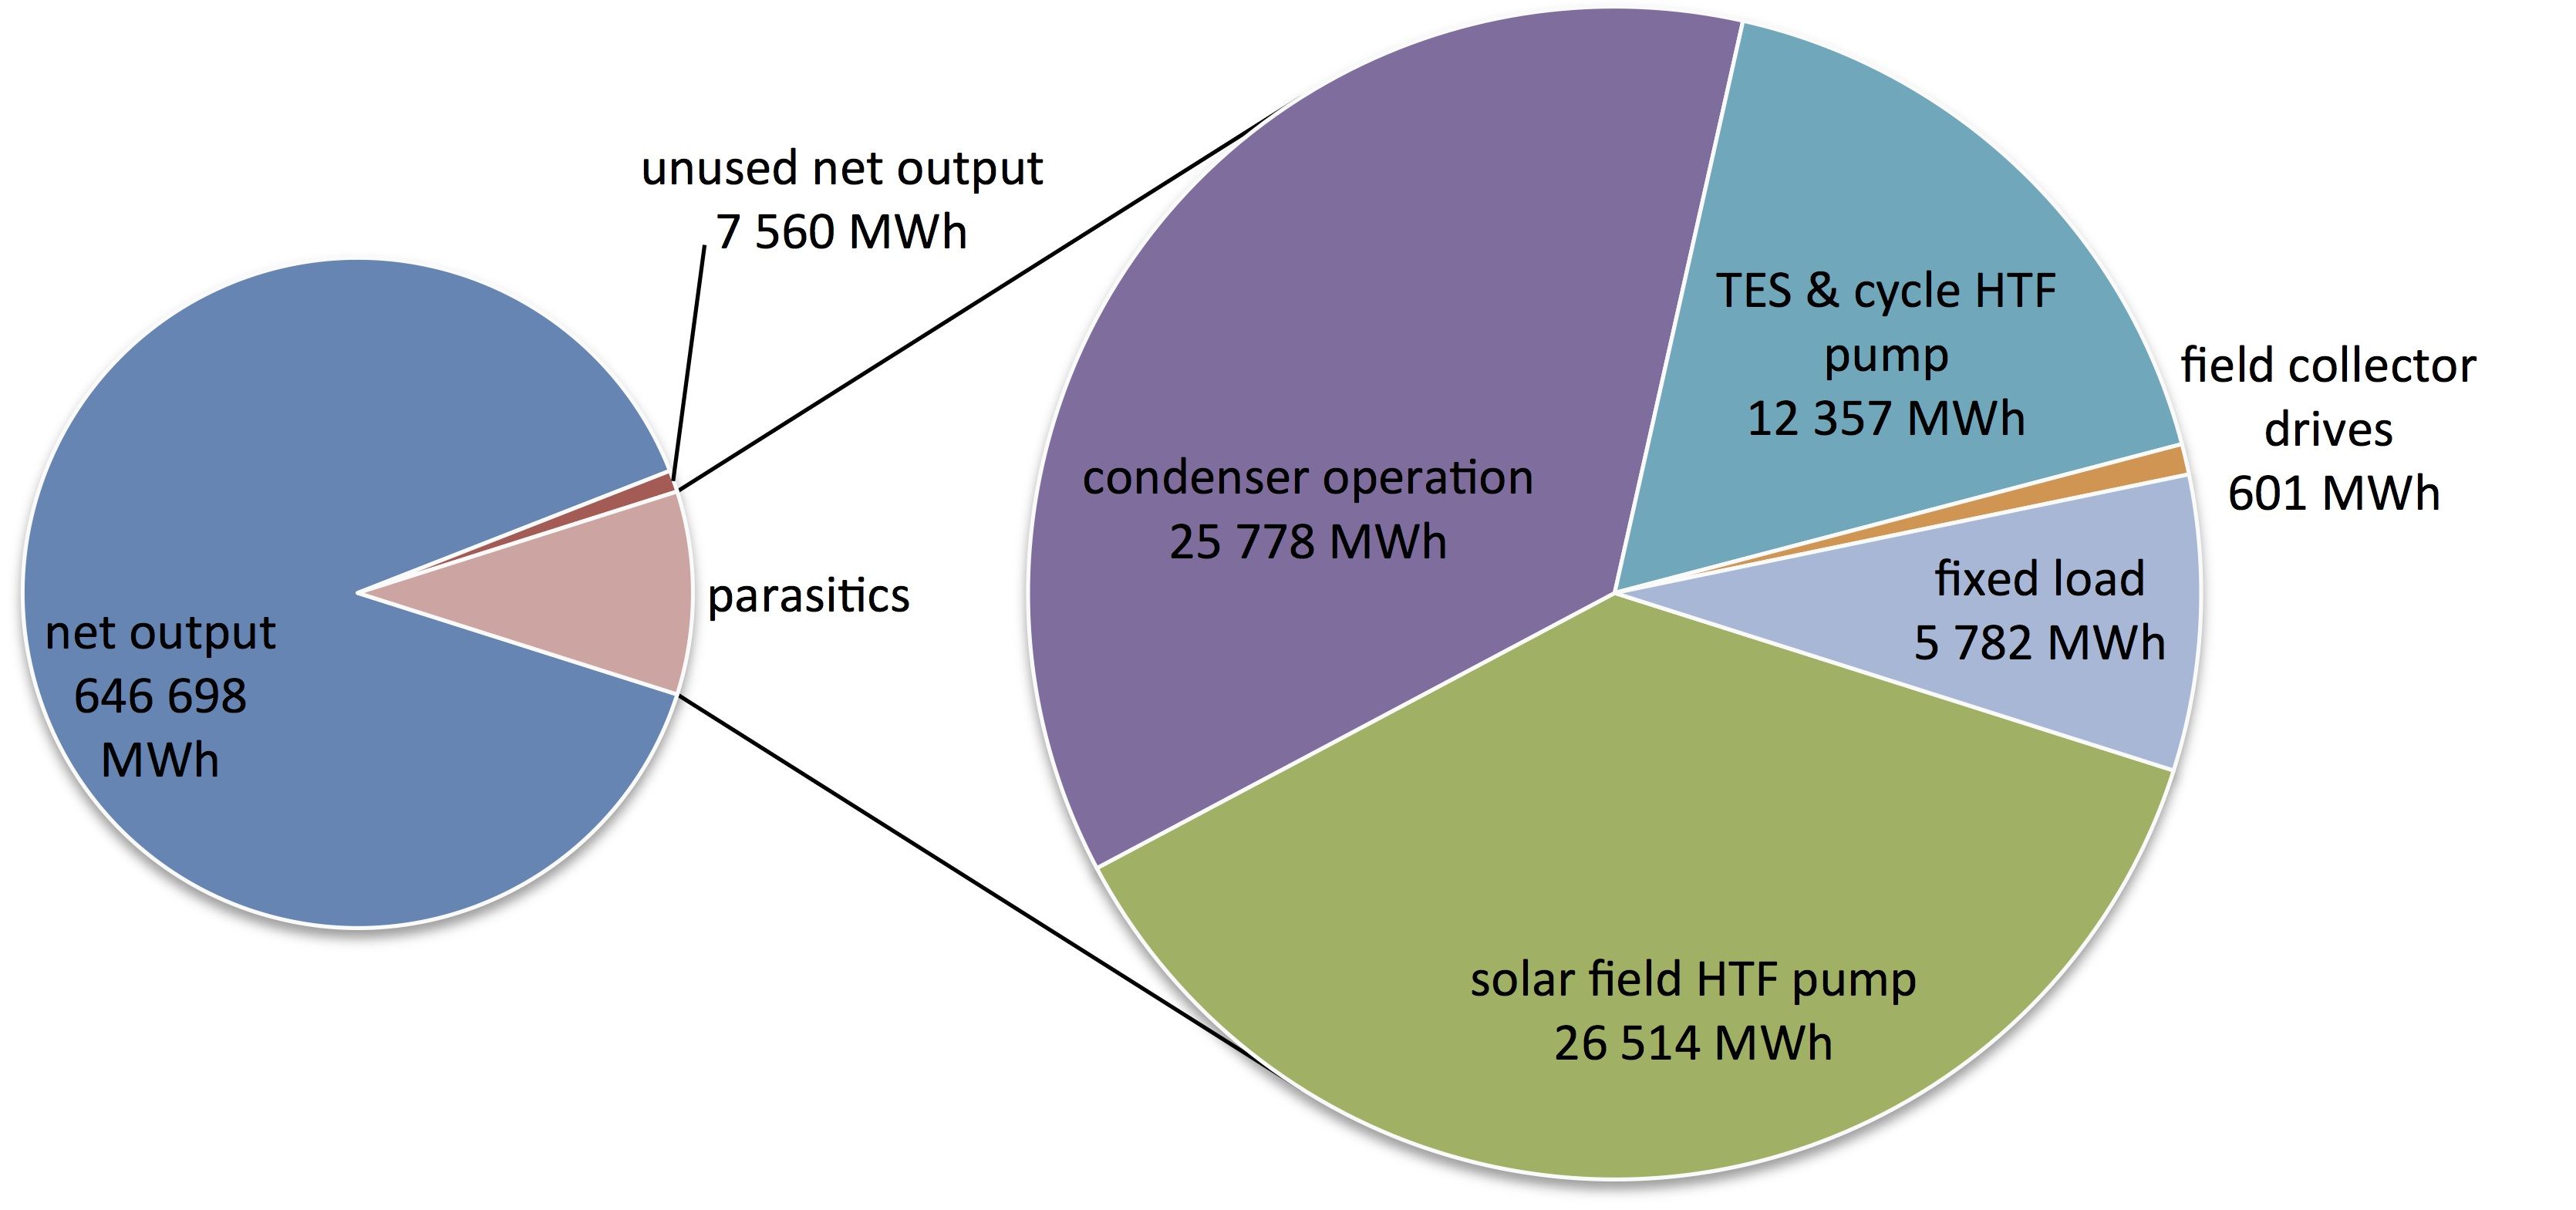
\includegraphics[width=1\textwidth]{FIG/PTC_parasitics_high}
                \caption{SM: 5.0 TES: 16 h}\label{PTC_parasitics_high}
        \end{subfigure}
        \caption[Share of annual gross energy output of selected PTC power plant configurations.]{Share of annual gross energy output of selected PTC power plant configurations.}\label{PTC_parasitics}
\end{figure}
Figure~\ref{PTC_parasitics_low} names the total net output for covering the prescribed load at about \SI{380.51}{GWh} for the PTC power plant with a SM of 2.0 and \SI{8}{h} of TES. The total sum of the annual prescribed load is \SI{711.75}{GWh}. Therefrom results a covering of 53.5~\% of the PTC power plant with the lowest configurations. The annual net output result of the highest simulated PTC configuration can be found in Figure~\ref{PTC_parasitics_high} and is about \SI{646.70}{GWh} which results in a load covering from about 90.9~\% over the year of the prescribed load. 

The remaining load covering results of all simulated PTC power plants can be found in Figure~\ref{PTC_LCCF}. The chart shows that at a SM of 2 all simulated TES variations reaching a load curve covering of 53.4~\%. It can be noteced that the growing rate of the covering is declining with the rising SM. The growing rate from the SM 2.0 to 2.5 is between 10.9~\% and 14.9~\% while it is from the SM 4.5 to 5.0 just between 1~\% and 2~\%. Also there is no noticeable gain between using 12, 14 or \SI{16}{h} of TES. The difference is at highest 0.7~\%. 

\begin{figure}[htbp]  
\centering
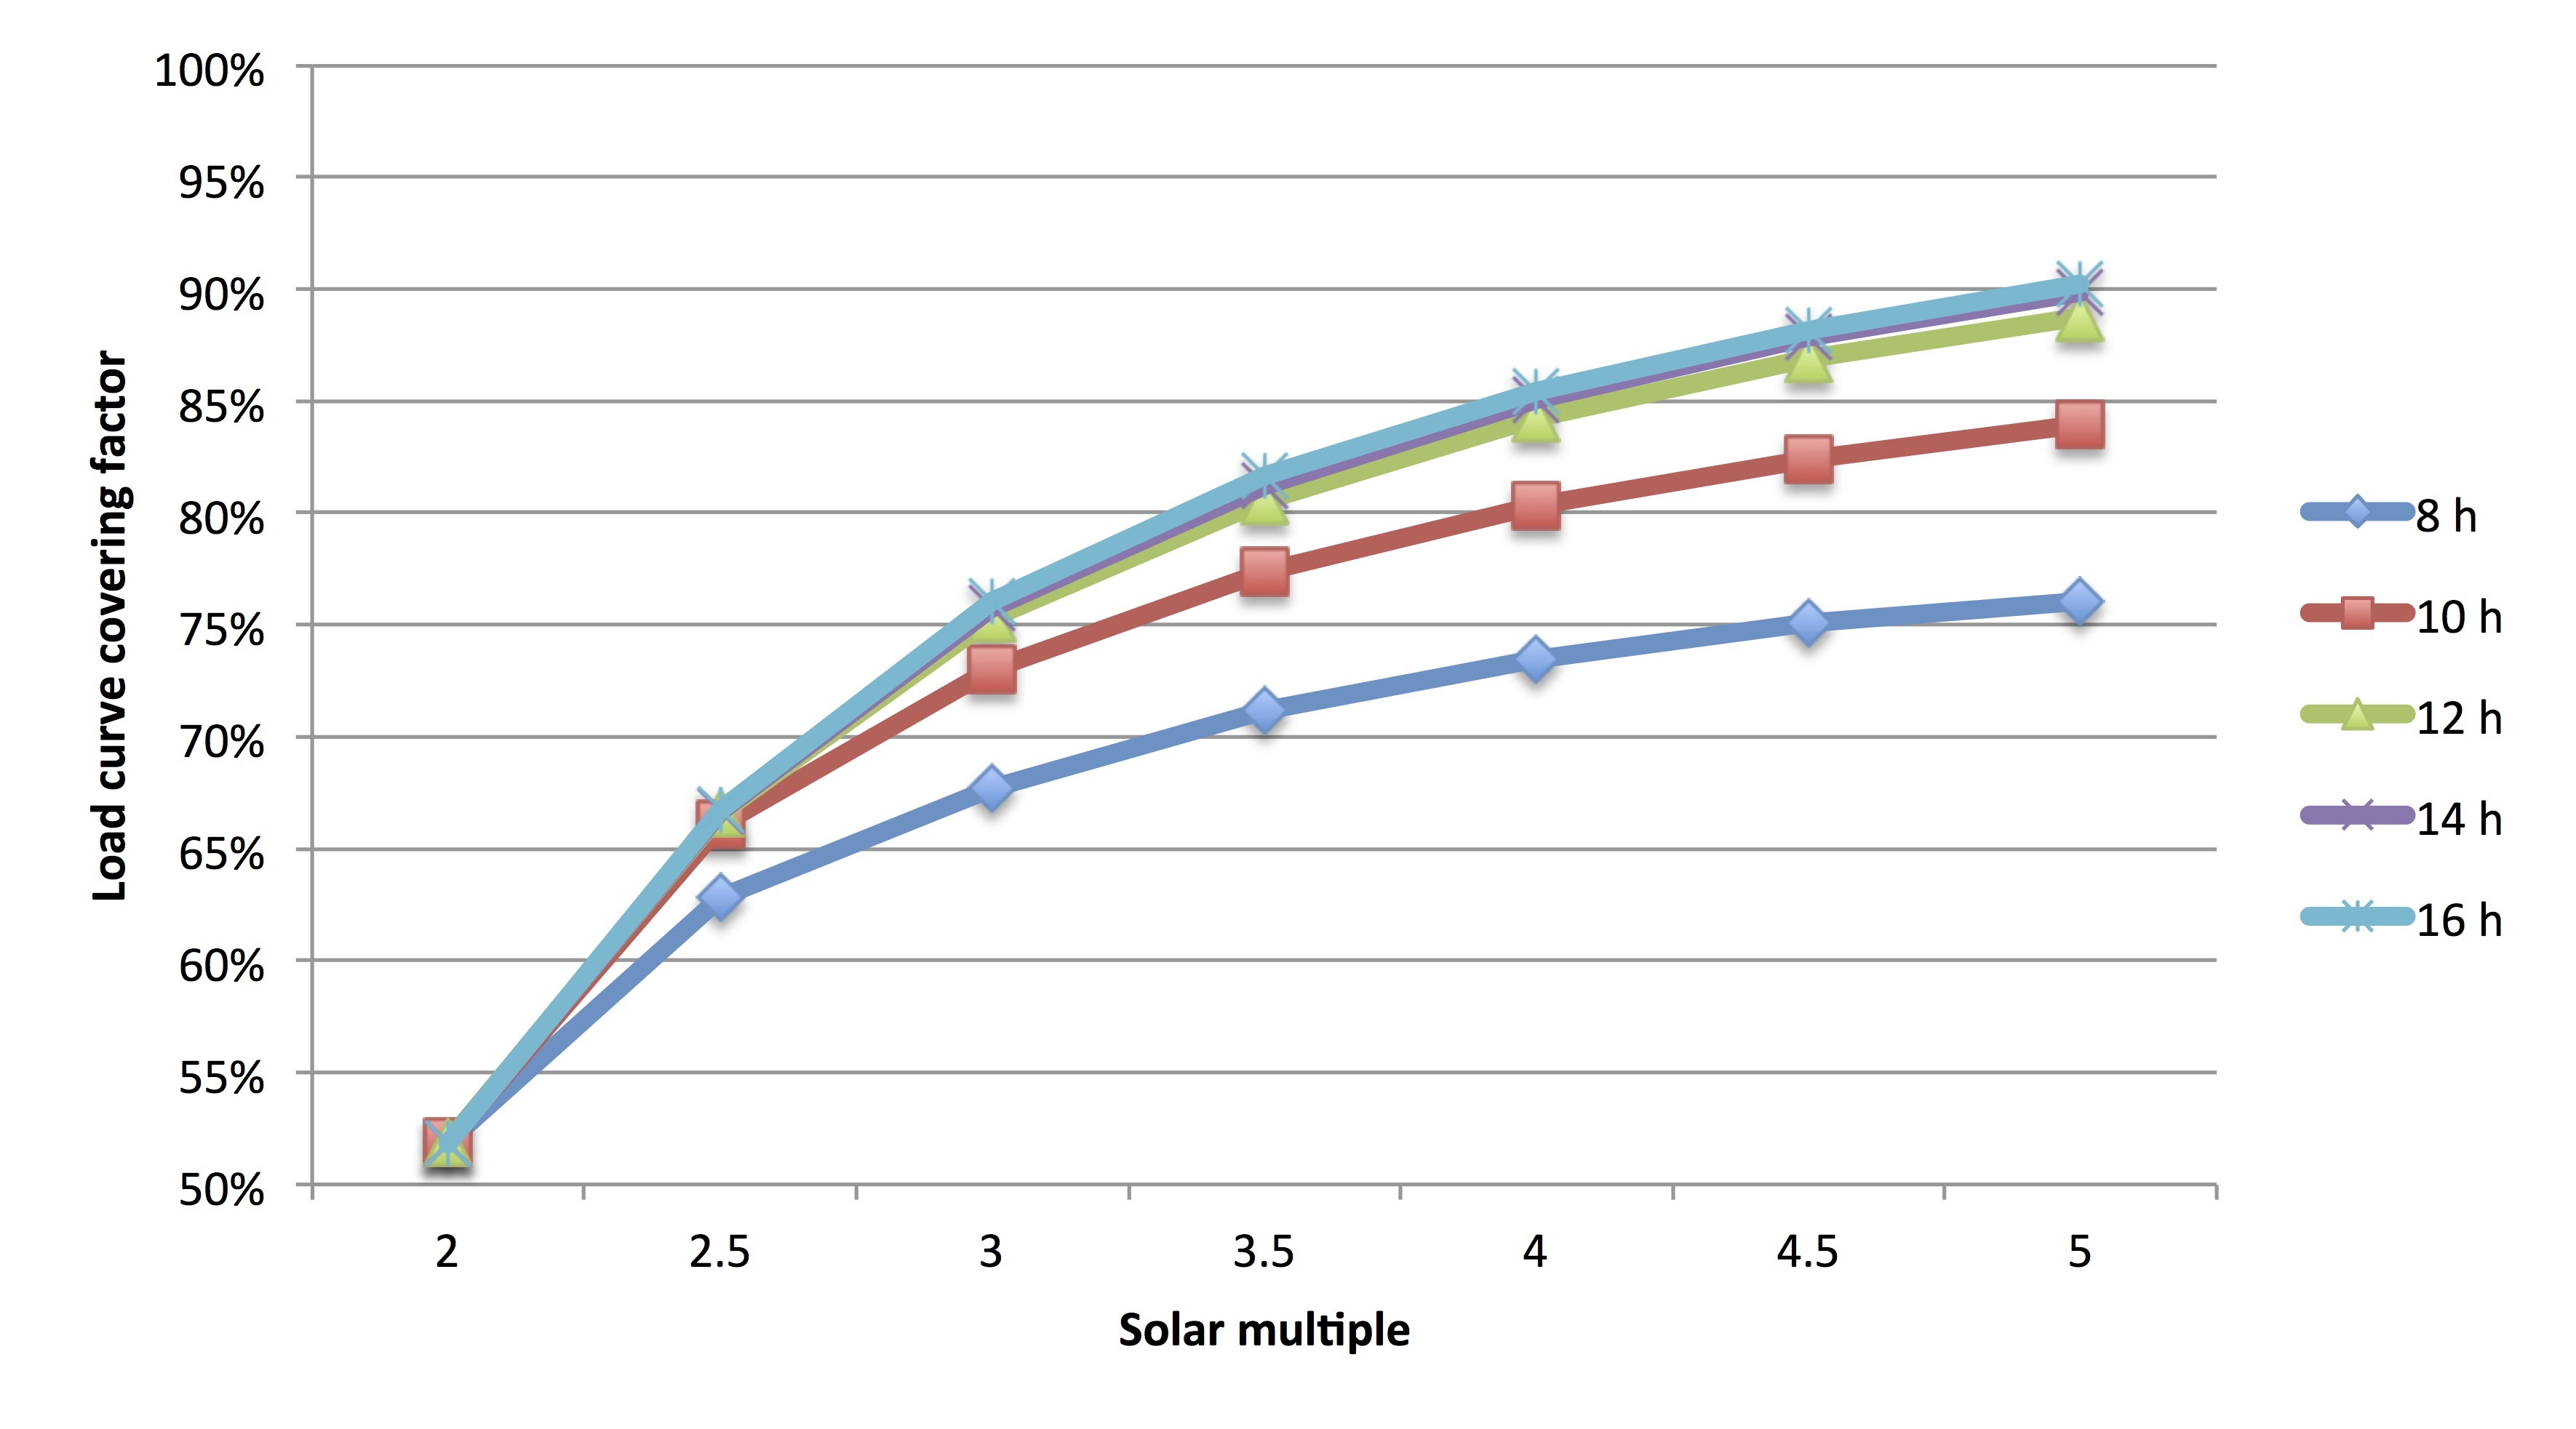
\includegraphics[width=1\linewidth]{FIG/PTC_LCCF}
\caption[Load curve covering result of simulated PTC systems.]{Load curve covering result of simulated PTC systems.}\label{PTC_LCCF}
\end{figure}
The target of 90~\% load covering is just reached by a SM of 5.0 and more then \SI{12}{h} of TES and it can be noted that it seams to be really elaborate for reaching that high value of annual covering using a PTC plant. 70~\% load covering was reached at all simulated PTC configurations. While 80~\% load covering was reached by all configurations besides the \SI{8}{h} of TES.
\subsubsection{Levelized costs of electricity}
For the calculated LCOE the finacial input parameter in Table~\ref{tbl: PTCFinance} and a simplified method which is documented in Appendix~\ref{ChapterLCOE} on Page \pageref{ChapterLCOE} was used. These results of the LCOE claculation for the simulated PTC configurations can be seen in Figure~\ref{PTC_LCOE}. 

The lowest LCOE result of the simulated PTC power plants is \SI{161.69}{USD/MWh} at a SM of 2.5 and \SI{8}{h} of TES. The \SI{10}{h} TES has marginal higher result using a SM of 3.0 (\SI{162.00}{USD/MWh}) and 2.5 (\SI{162.35}{USD/MWh}). The highest LCOE result of \SI{216.63}{USD/MWh} was reached at a SM of 2.0 and \SI{16}{h} of TES. 

Depending from almost identical load curve covering is the behavior of LCOE results of the simulated TES variations 12, 14 and \SI{16}{h} almost identical. The difference in the height of the charts results from the higher investment cost of the larger storage configuration.

\begin{figure}[htbp]  
\centering
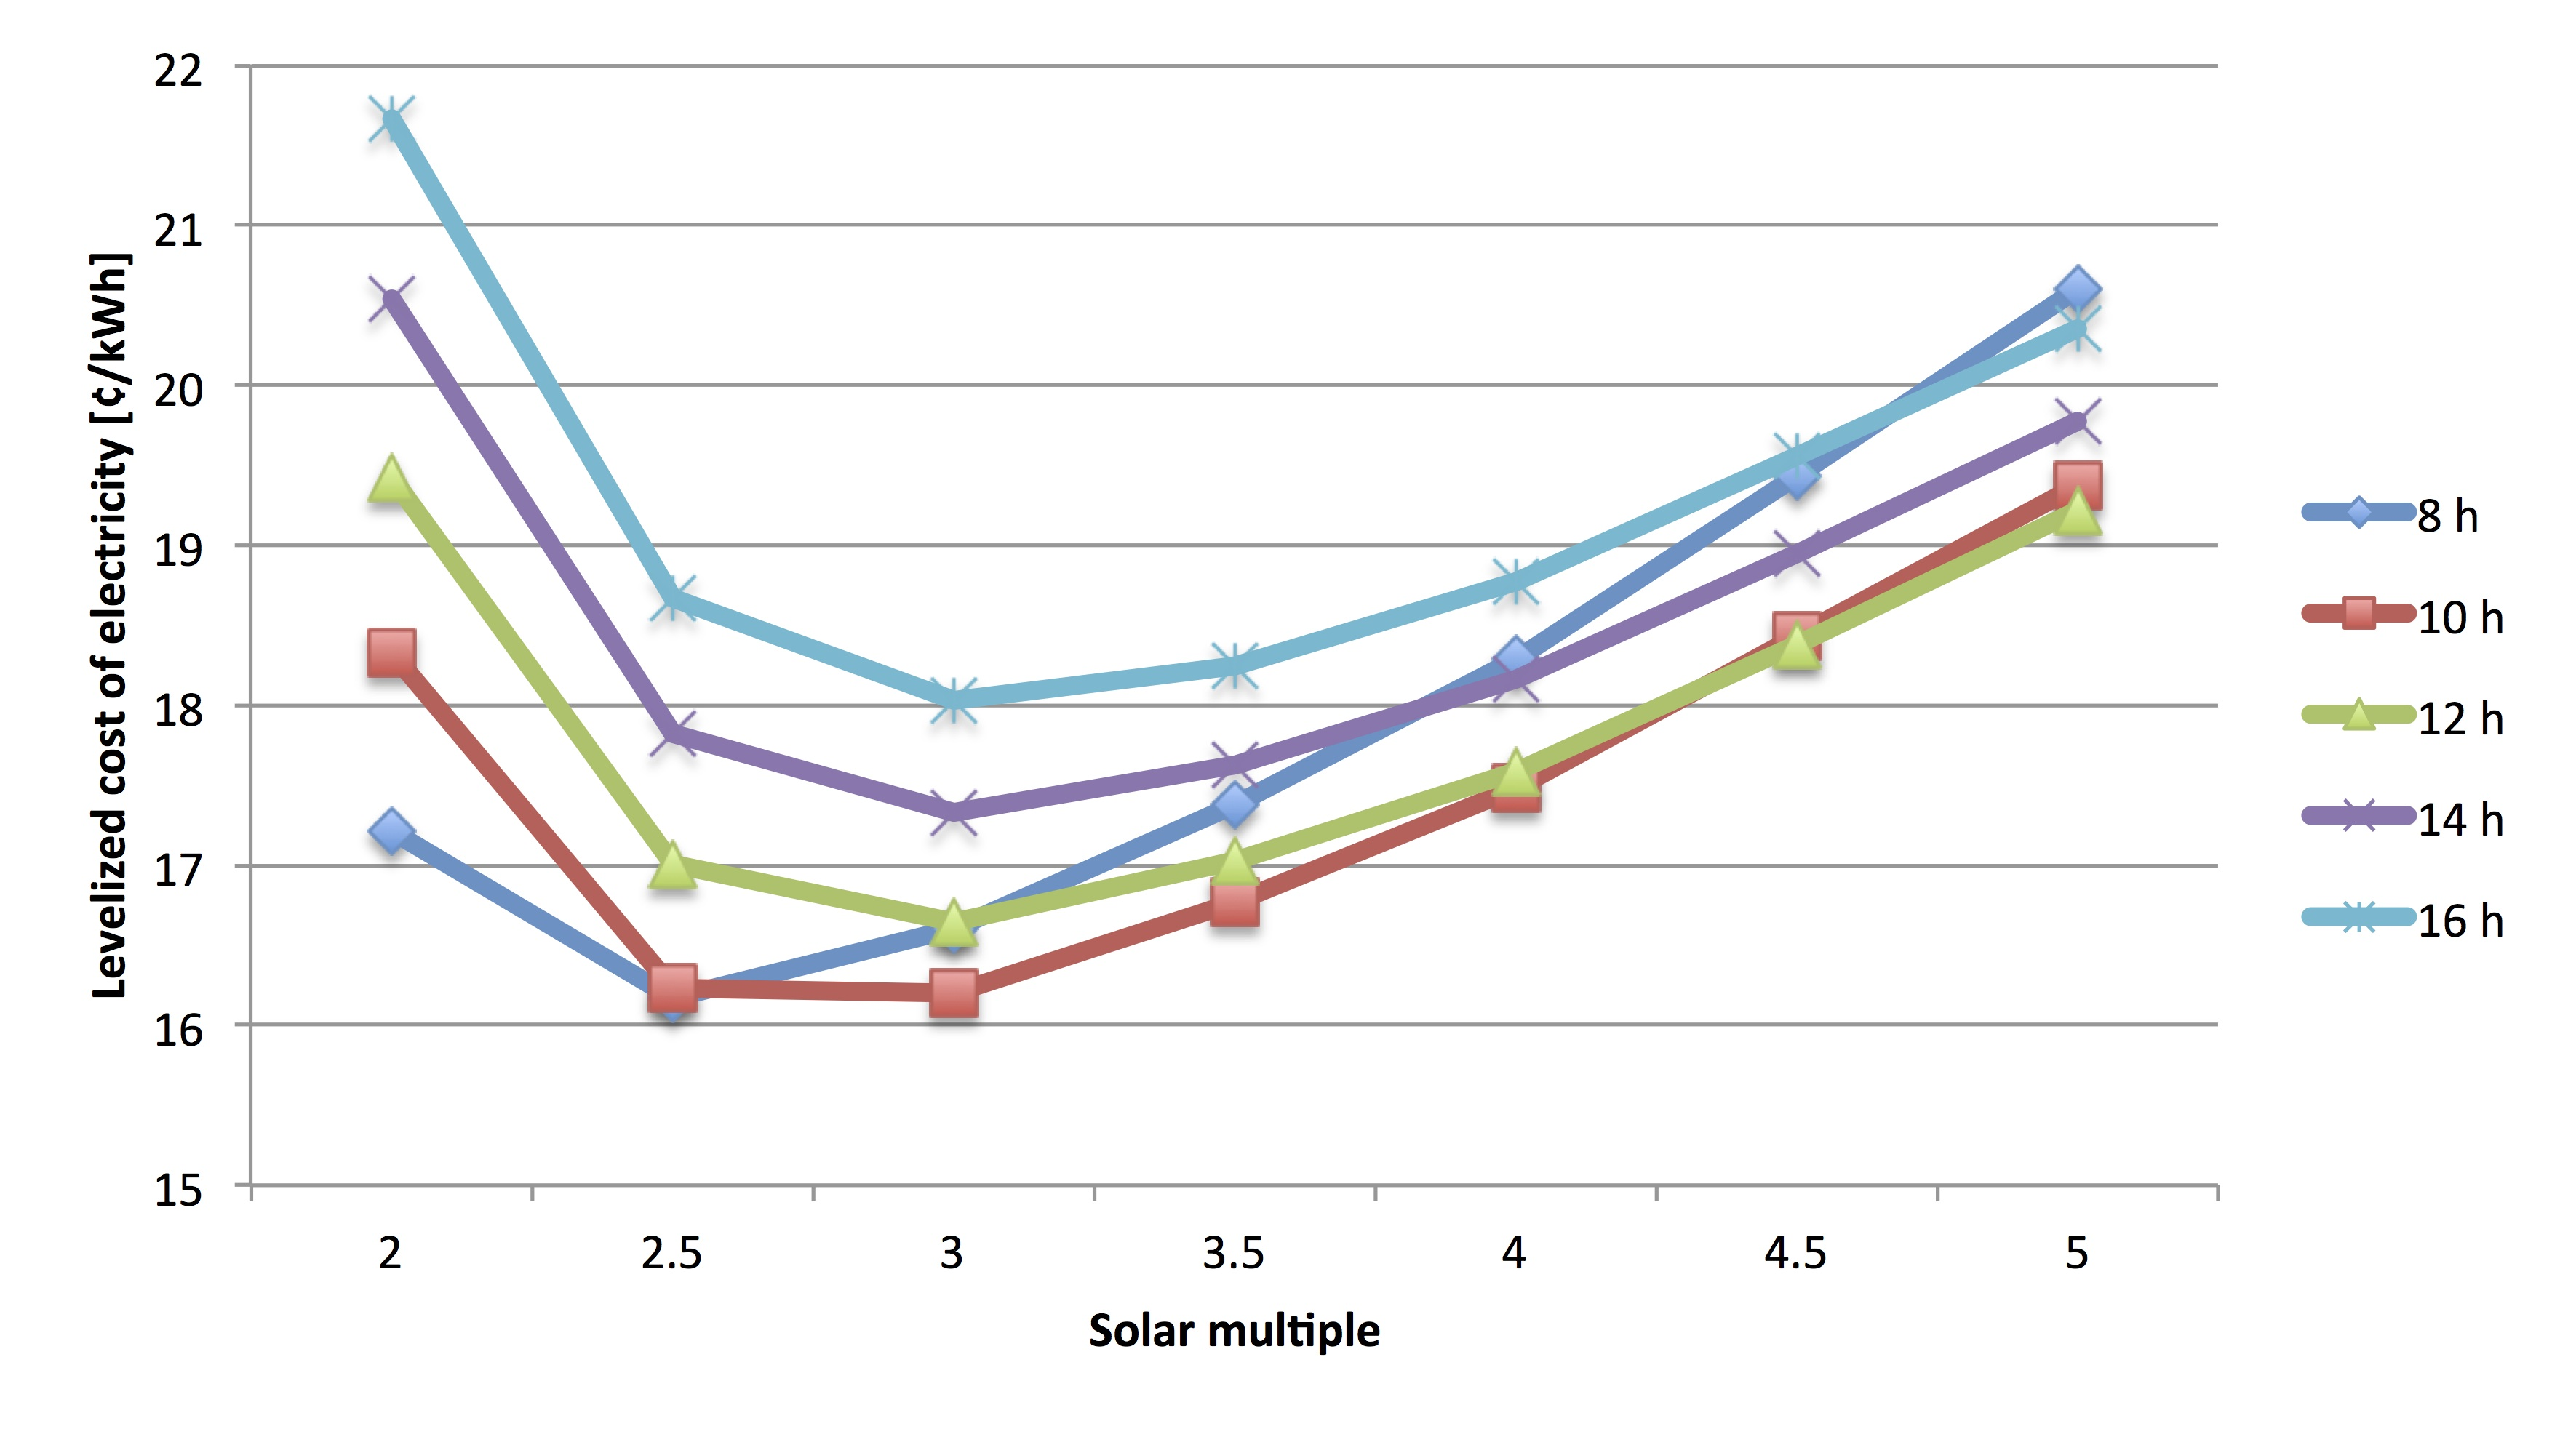
\includegraphics[width=1\linewidth]{FIG/PTC_LCOE}
\caption[LCOE calculation results for PTC simulation.]{LCOE calculation results for PTC simulation.}\label{PTC_LCOE}
\end{figure}
The calculated annual LCOE's of the simulated PTC power plants are composed by six cost parts, namely the investment costs of the collector field, TES, power block, land purchase and additional EPC, project management (PM) and risk as well as the annual operation and maintenance (O\&M) costs. The share of the annual LCOE for the selected PTC power plants can be seen in Figure~\ref{PTC_LCOE_BreakDown}. The share of the land purchase is almost irrelevant for the LCOE. 

When comprising the load curve covering results and the LCOE calculation results of the simulated PTC power plants, the lowest LCOE for reaching the target of 90~\% load curve covering is \SI{192.15}{USD/MWh} at a SM of 5.0 and \SI{16}{h} of TES. 

For reaching a covering of 80~\% of the load curve the PTC configuration with a SM of 3.5 and \SI{12}{h} of TES has the lowest LCOE with \SI{170.32}{USD/MWh}. The lowest LCOE for reaching 70~\% of the prescribed load curve is \SI{162.00}{USD/MWh} at a SM of 3.0 and \SI{10}{h} of TES.
\begin{figure}[!htbp]
        \centering                
        \begin{subfigure}[b]{0.5\textwidth}
                \centering
                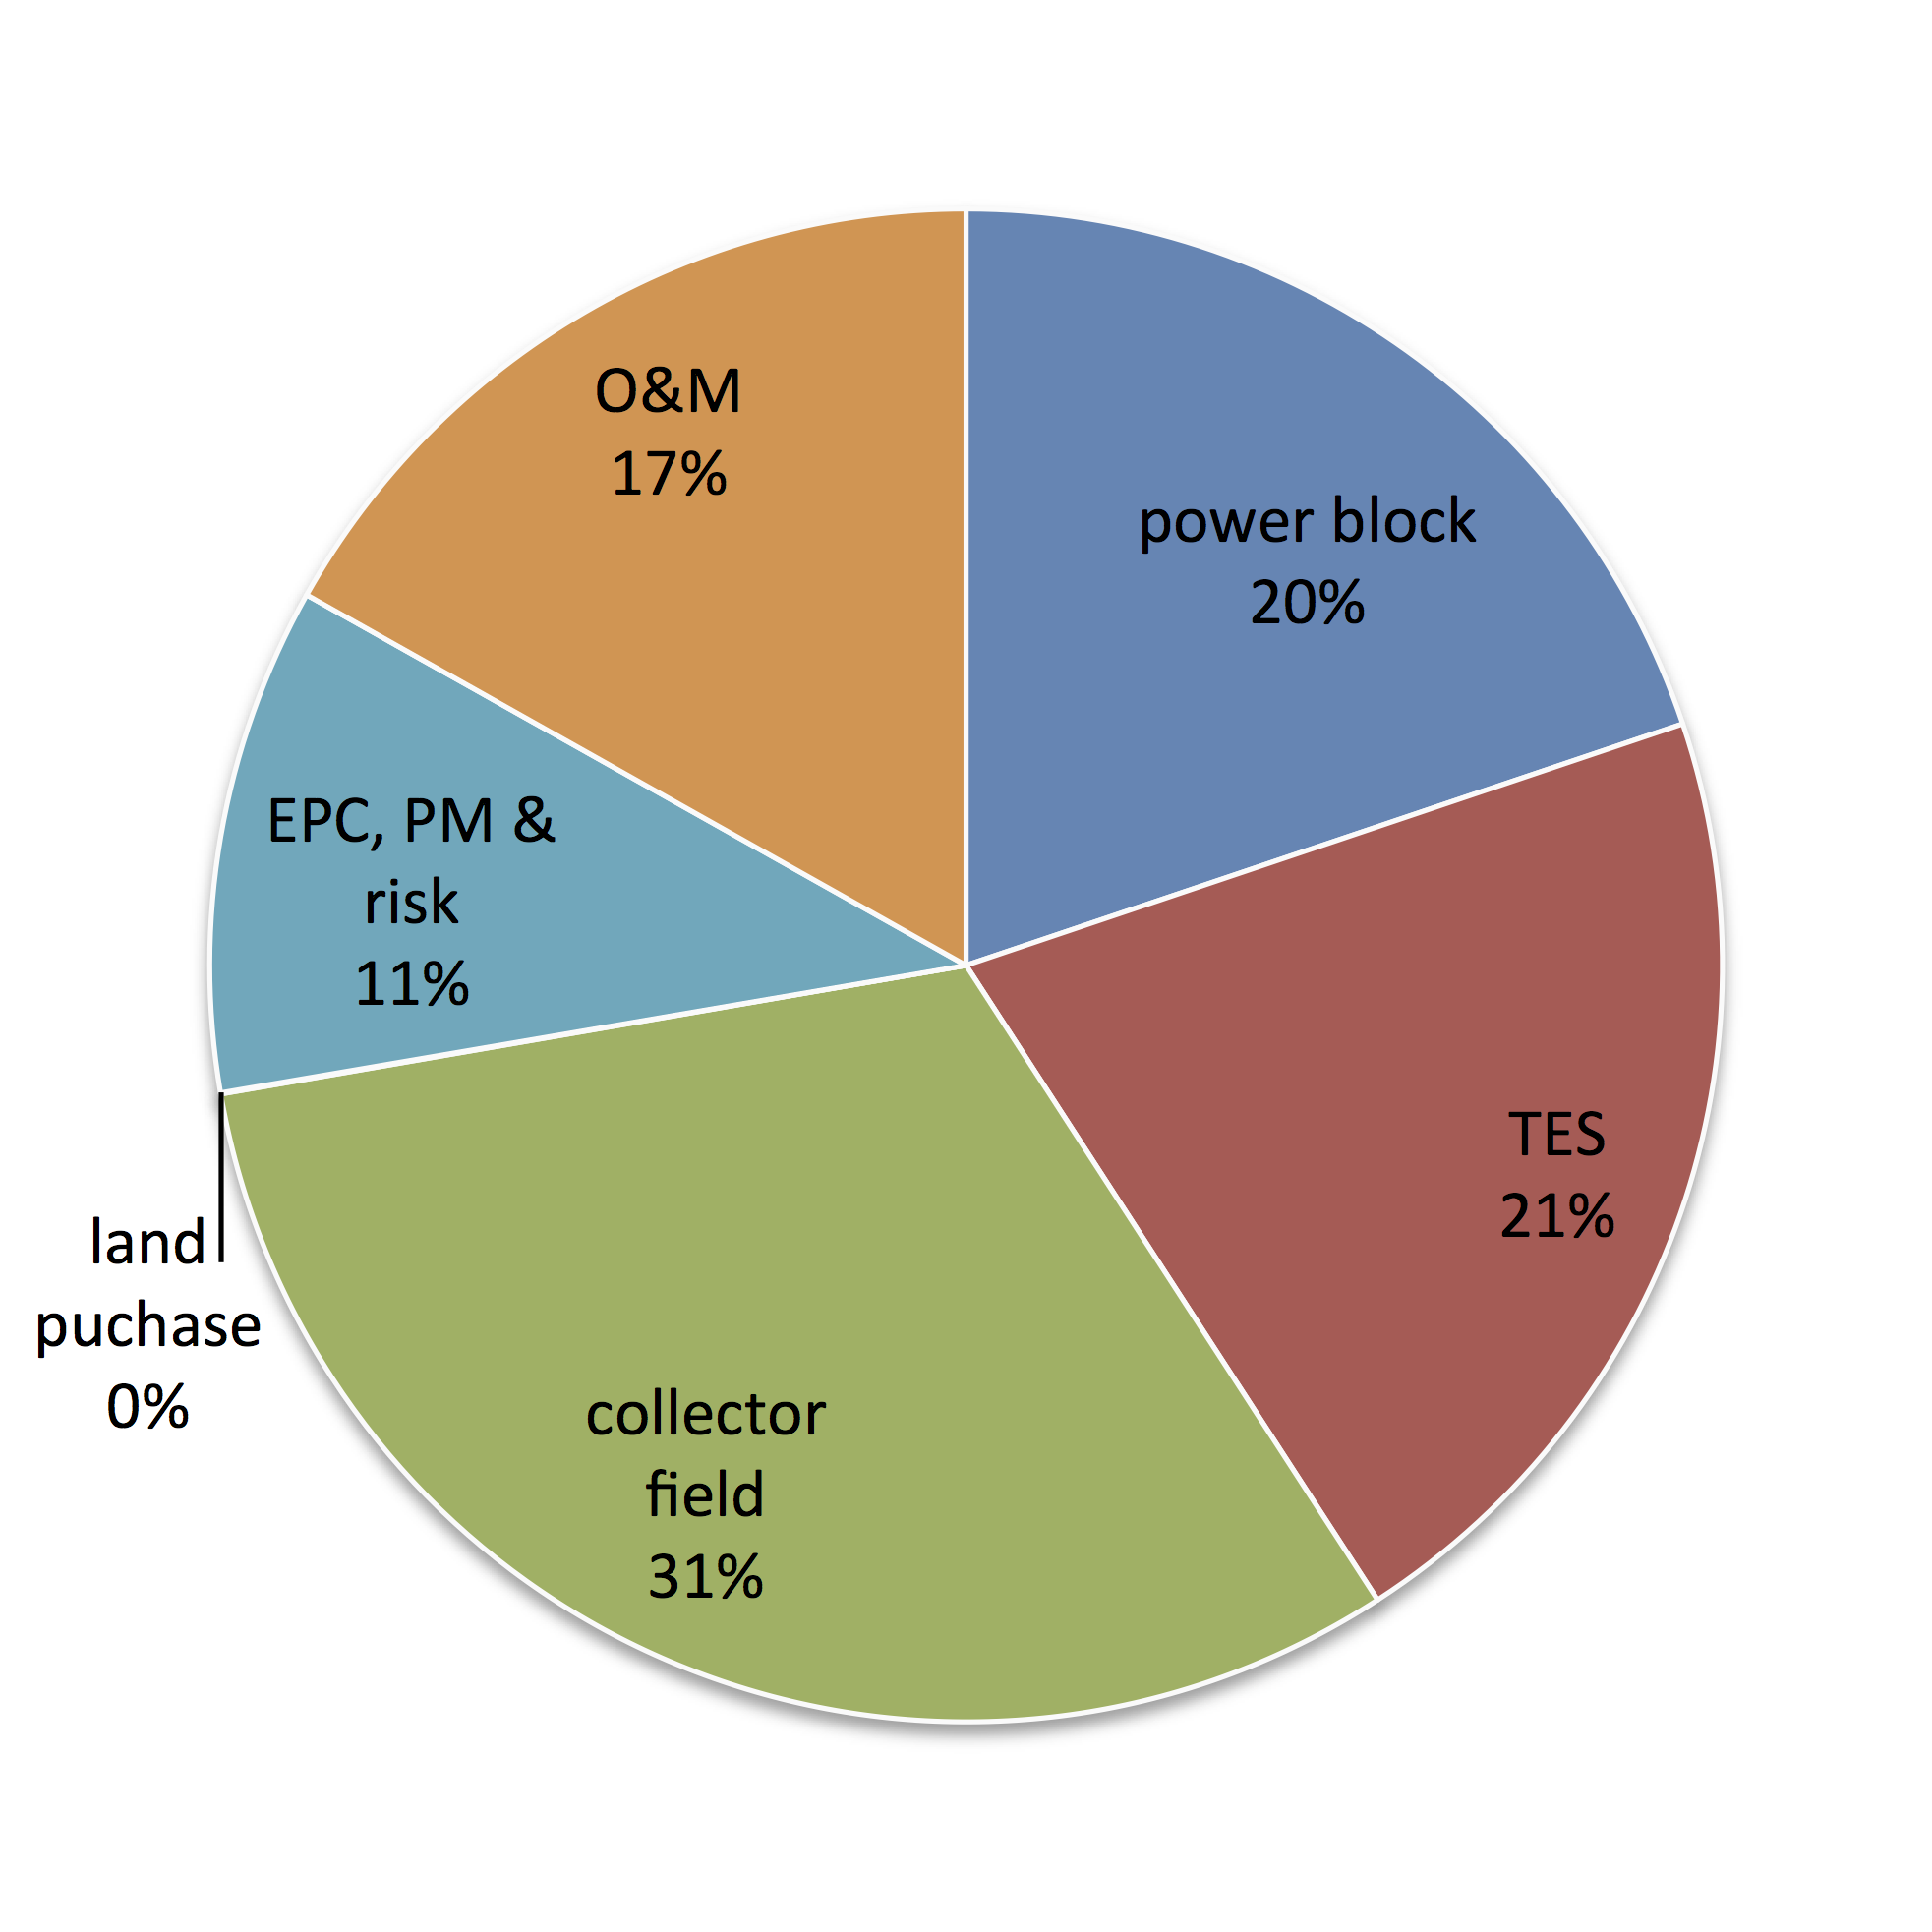
\includegraphics[width=1\textwidth]{FIG/PTC_LCOE_lowinvest_BreakDown}
                \caption{LCOE break-down for SM~2.0 and \SI{8}{h}~TES.}\label{PTC_LCOE_lowinvest_BreakDown}
        \end{subfigure}%
        ~
        \begin{subfigure}[b]{0.5\textwidth}
                \centering
                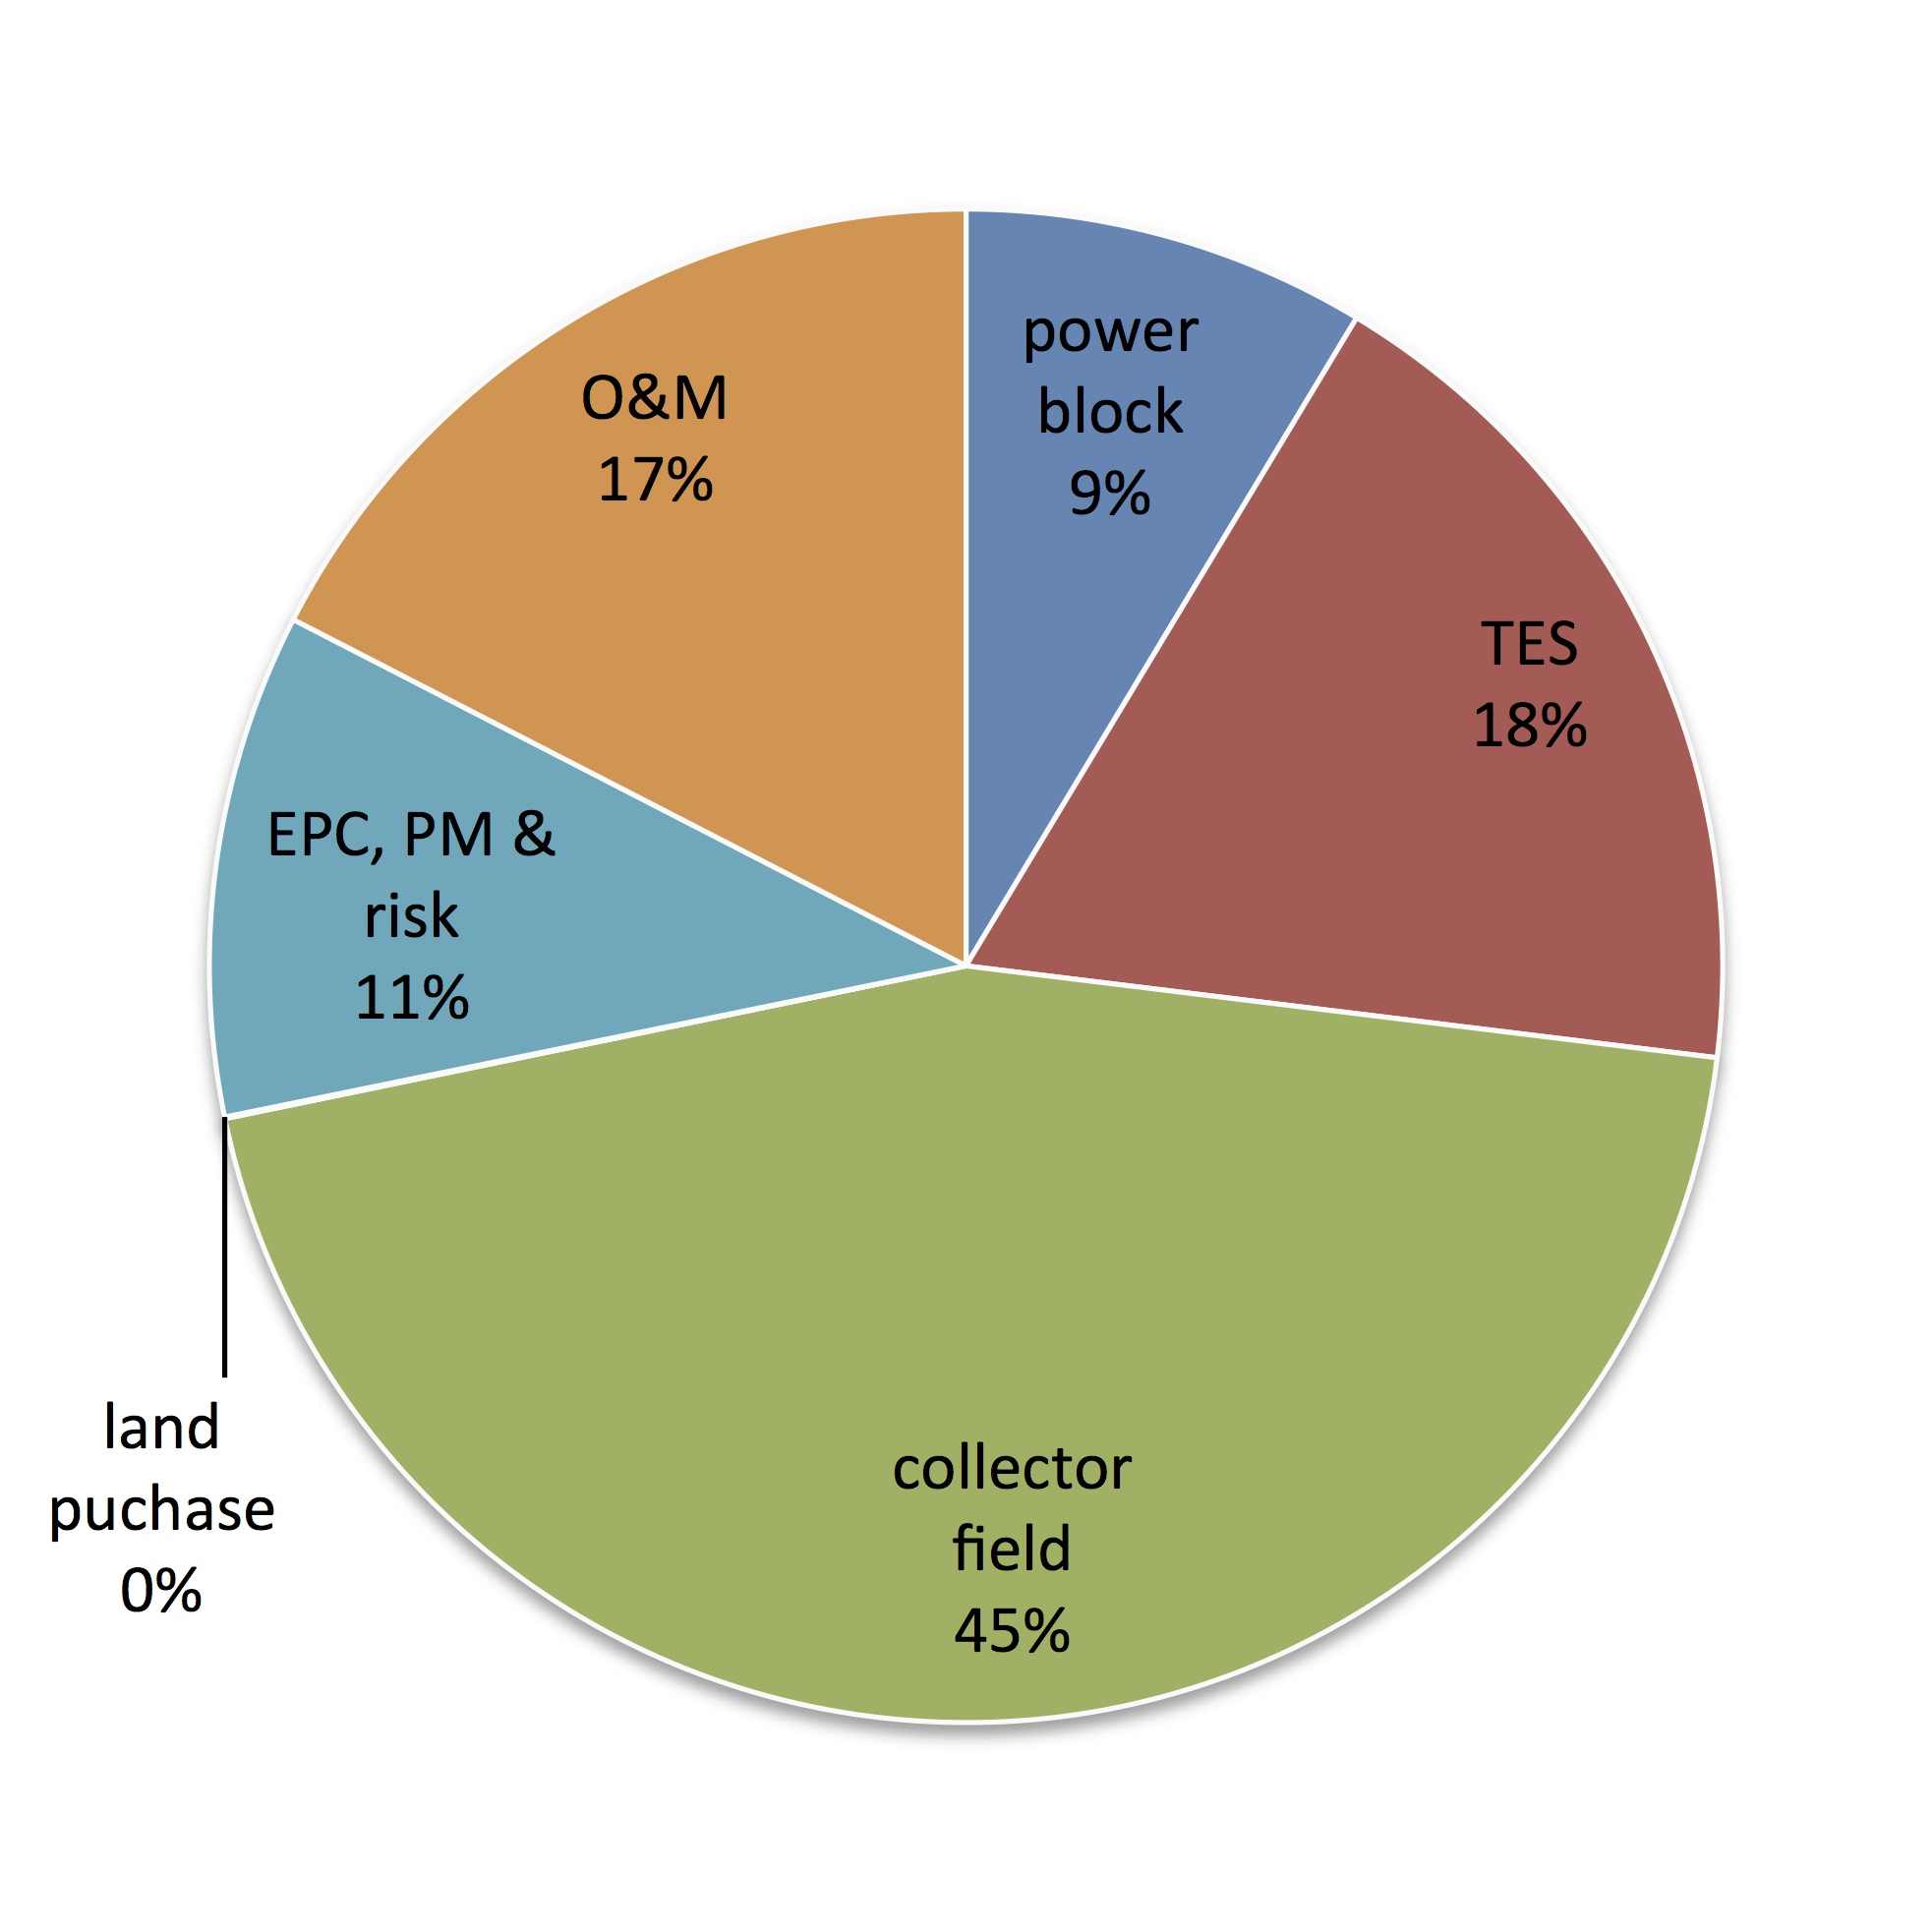
\includegraphics[width=1\textwidth]{FIG/PTC_LCOE_highinvest_BreakDown}
                \caption{LCOE break-down for SM~5.0 and \SI{16}{h}~TES.}\label{PTC_LCOE_highinvest_BreakDown}
        \end{subfigure}
        \caption[Break-down of selected PTC-LCOE calculation results.]{Break-down of selected PTC-LCOE calculation results.}\label{PTC_LCOE_BreakDown}
\end{figure}
\pagebreak
\section{PV power plant with adapted EES}
\subsection{Design and simulation} \label{section PV system}
For this simulation a PV power plant was extended with an electrical energy storage (EES). This extended PV power plant was simulated in SAM's "Photovoltaic (detailed)" model with enabled battery storage option. Also for this simulation was the EPW weather file for Upington from Section~\ref{Location and weather data} used. For the PV simulation SAM uses the following input data:
\begin{itemize}
\item Latitude ($\,^{\circ}$)
\item Longitude ($\,^{\circ}$)
\item Elevation above sea level (m)
\item GHI, DNI and DHI (\si{\watt\per\square\metre})
\item Dry bulb temperature (\si{\celsius})
\item Wind velocity (\si{\metre\per\second})
\end{itemize}
This section describes in detail the residual input data of the PV power plant with adapted battery storage. As before in the sections of simulated CSP technologies first the essential components of the system are defined. The financial parameters and the LCOE for this simulation was also here calculated separately and is documented in Appendix~\ref{ChapterLCOE} on Page \pageref{ChapterLCOE}.



As mentioned at the beginning of these Chapter this must be seen as theoretical simulation. Actually there are not that large electrical energy storage systems in form of battery storage available.



For this simulation the load was conected to the PV and Battery system as shown on Figure~\ref{PV_model_config}. The load shape was defined as before specified before in Chapter~\ref{Overall simulated configuration} and simulates the demand of the power grid. As it is shown there is also the actual power grid connected as additional component, but for this simulation just the power flows between PV, battery and load is in focus. As it is shown in the Figure, SAM actually just support the battery connection at the AC-bus via a power conversion system and is not able to simulate direct DC-connected batteries besides the PV-array before the PV-inverter. However in order to produce comparable results SAM was also used for the simulation of the PV power plant. As mentioned before this system contains out of the PV system with solar modules, solar and inverter and are described in the following section as well as the electrical energy storage.
\begin{figure}[htbp]  
\centering
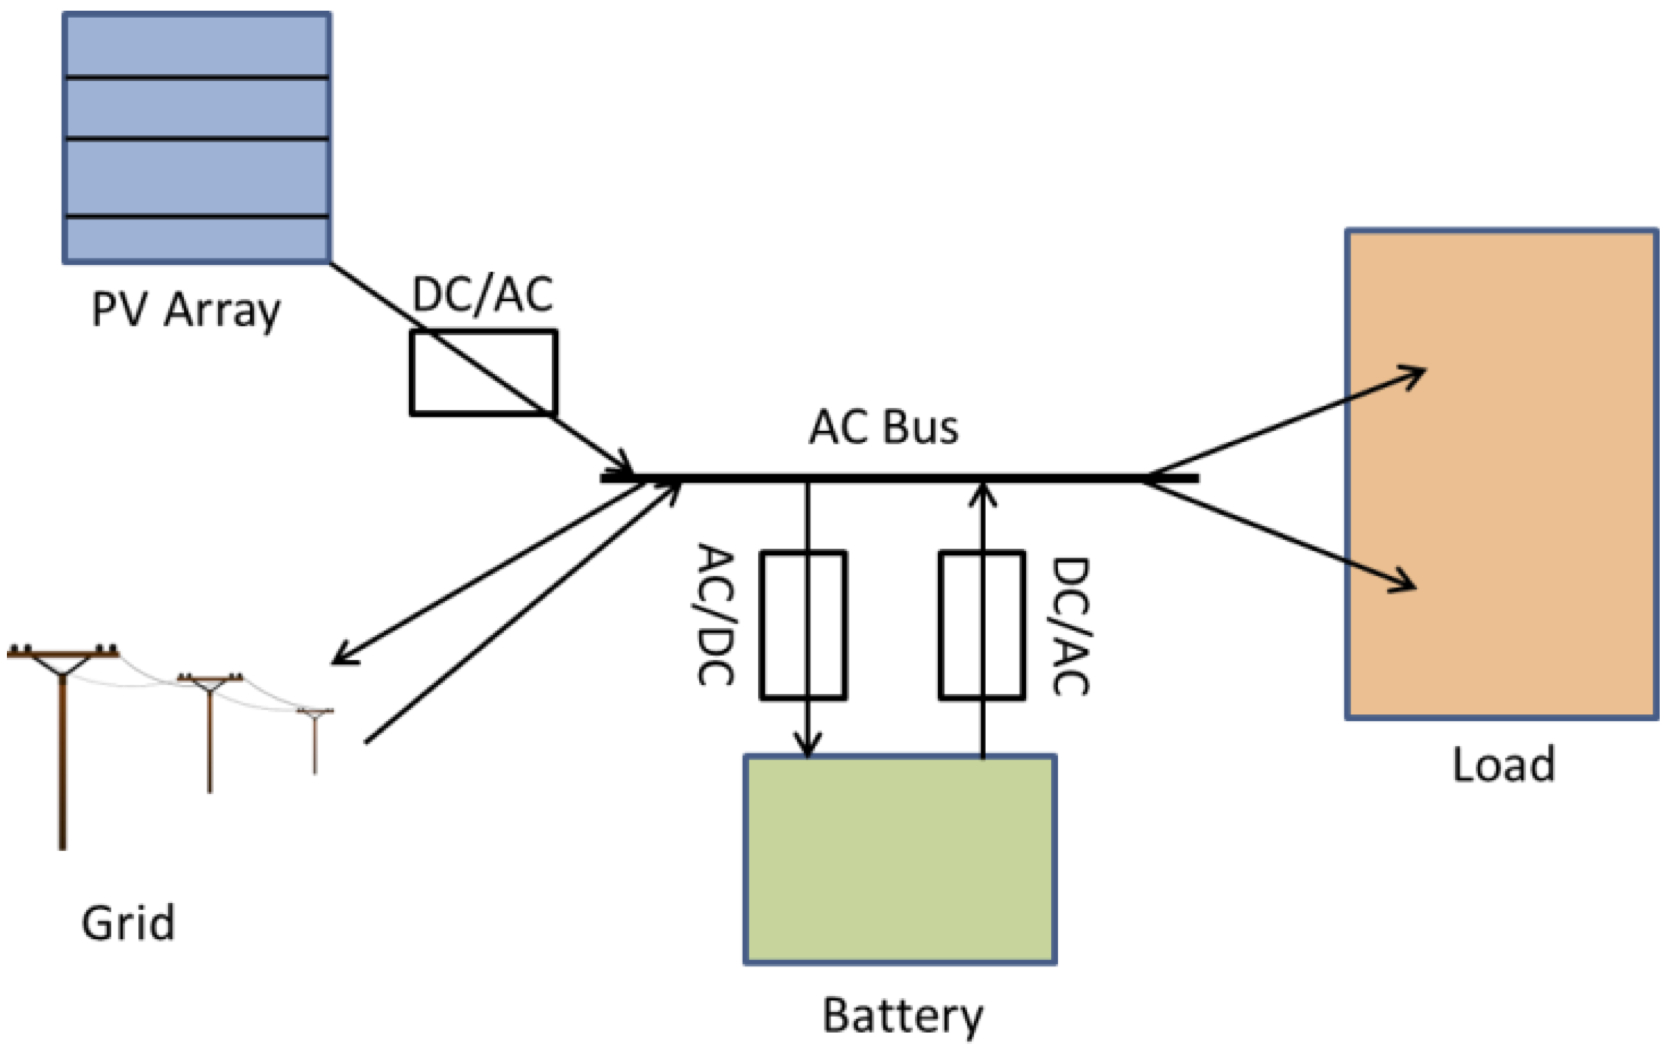
\includegraphics[width=0.55\linewidth]{FIG/PV_model_config}
\caption[Model of the configurated PV plus batterie scheme.]{Model of the configurated PV plus batterie scheme \cite{Diorio2015}.}\label{PV_model_config}
\end{figure}
\subsubsection{Simulated configurations}
The configurations of the PV system with adapted electrical energy storage has also the target to reach 90~\% of the scheduled production curve from Section~\ref{Overall simulated configuration}. To reach this target it is necessary to over scale the energy production of the PV system to produce enough power to covers the given load and load the storage during the day. This is quite similar to the solar multiple of the CSP system, but can not be put on a same level. Therefore this over scaling will be called "PV multiple" (PVM) and means the multiple of the PV inverter output. For example the system with a maximum inverter output of \SI{100}{\mega\wattel} is a PVM of 1 than has the PV system with a PVM of 2 a maximum inverter output of \SI{200}{\mega\wattel}. 
\begin{table}[htbp]  
  \centering
	\begin{tabular}{ p{4.0cm}  C{1.0cm} C{0.3cm} C{0.3cm} C{0.3cm} C{0.3cm} C{0.3cm}  | C{0.3cm} C{0.3cm} C{0.3cm} C{0.3cm} C{0.3cm} } 
	\hline	
\textbf{Item} & \textbf{Unit} & \multicolumn{10}{c}{\textbf{Value}} \\ \hline \hline
Maximum load supply & \si{\mega\wattel} & \multicolumn{10}{c}{100} \\ \hline
PV multiple & - & \multicolumn{5}{c}{1.0} & \multicolumn{5}{c}{1.8} \\
EES capacity & h & \multicolumn{5}{c}{-} & 4 & 5 & 6 & 7 & 8 \\ \hline 
PV multiple & - & \multicolumn{5}{c}{2.0} & \multicolumn{5}{c}{2.2} \\
EES capacity& h &  4 & 5 & 6 & 7 & 8 & 4 & 5 & 6 & 7 & 8 \\ \hline 
PV multiple & - & \multicolumn{5}{c}{2.4} & \multicolumn{5}{c}{2.6} \\
EES capacity & h & 4 & 5 & 6 & 7 & 8 & 4 & 5 & 6 & 7 & 8 \\ \hline 
\end{tabular}
\caption[Simulated configurations of the PV system with adapted EES.]{Simulated configurations of the PV system with adapted EES.}\label{tbl: PV_OverallConfig}
\end{table}
The simulated system load is maximum \SI{100}{\mega\wattel}, so this is also the maximum supply of the system. The PV system was simulated one time without storage and a maximum inverter output of \SI{100}{\mega\wattel} which is a PVM of 1. After that, the system was simulated in steps 0.2 of the PVM from 1.8 to 2.6. The adapted energy storage capacity was simulated from 4 to 8 hours in hourly steps. This storage capacity range is also defined for large-scale off-grid application in \cite{IEA2014c}. Table~\ref{tbl: PV_OverallConfig} summarizes the simulated configurations.
\subsubsection{PV system}
The simulated PV system is orientated at actual PV systems in SA. Therefore the currently under construction situated Mulilo Sonnedix Prieska PV Project in the Northern Cape will serve as a role model for the main components. In this \SI{75}{\mega\wattsdc}-project are poly crystalline \SI{305}{\wattsdc} modules of type BYD 305P6C-36 from BYD installed. The efficiency of the modules is about 15.72~\%. The full module specification is in Table~\ref{tbl: PVmodule}. The peak performance of the project is \SI{86.23}{\mega\wattsdc}. \cite{Morse2014}

\begin{table}[htbp]  
  \centering
	\begin{tabular}{  p{5.0cm}  C{5.0cm}  C{1.4cm} } 
	\hline	
\textbf{Item} & \textbf{Value} & \textbf{Unit} \\ \hline \hline
Manufacturer  & BYD COMPANY LIMITED & - \\ 
Model & BYD 305P6C-36 & - \\ 
Cell type &  poly-crystalline silicon & - \\ \hline
Maximum power & 304.99 & \si{\wattel} \\ 
Nominal efficiency & 15.72 & \si{\percent} \\ 
Maximum power voltage & 36.2 & \si{\voltsdc} \\ 
Maximum power current & 8.4 & \si{\ampsdc}  \\
Open circuit voltage & 45.5 & \si{\voltsdc}  \\ 
Short circuit current & 8.9 & \si{\ampsdc}  \\
Temperature efficiency & -0.41 & \si{\percent\celsius}\\
Module area & 1.94 & \si{\square\metre} \\ 
Number of cells & 72 & -\\
\hline
\end{tabular}
\caption[Module specification of BYD 305P6C-36.]{Module specification of BYD 305P6C-36 under STC: \SI{1000}{\watt\per\square\metre}, cell temperature \SI{25}{\celsius} \cite{NREL2015g}.}\label{tbl: PVmodule}
\end{table}


These for the simulation selected module type was already deposited in the module library in SAM. This large library is based on the database of Go Solar California for photovoltaic modules and inverters from the California Energy Commission \cite{NREL2015g}.

\begin{figure}[htbp]  
\centering
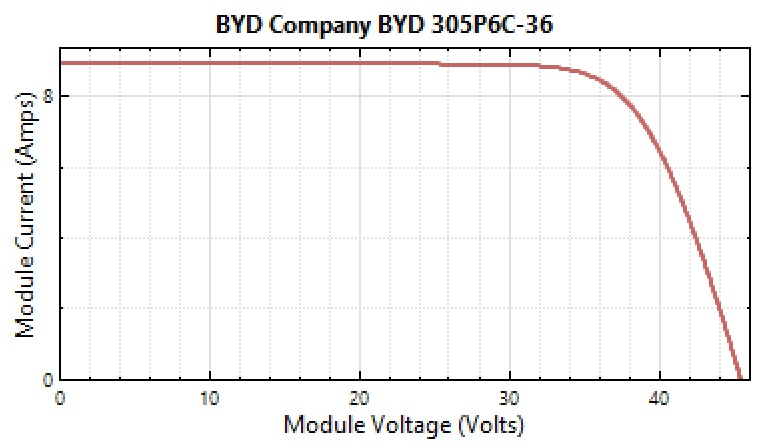
\includegraphics[width=0.70\linewidth]{FIG/PVModuleVA}
\caption[Current–voltage characteristic under STC of module BYD 305P6C-36.]{Current–voltage characteristic under STC of module BYD 305P6C-36 \cite{NREL2015g}.}\label{PVModuleVA}
\end{figure}


Figure~\ref{PVModuleVA} shows the module’s current–voltage characteristic with a short circuit voltage of \SI{8.9}{A} and an open circuit voltage of \SI{45.5}{V}.\newpage\noindent
The Mulilo Sonnedix Prieska PV Project install inverter from AEG. These specific AEG Protect PV.800 inverter is not available in the library of SAM, but a similar model with almost the same power rating was selected. Table~\ref{tbl: PVinverter} depicts the specifications of the for the simulation used Ingeteam inverter INGECON SUN 805TL U X420 Outdoor with \SI{805}{kW}\textsubscript{ac} power at an efficiency of 98.33~\%. The efficiency curve of the inverter can be seen in Figure~\ref{InverterEfficiencyCurve}. 

\begin{figure}[htbp]  
\centering
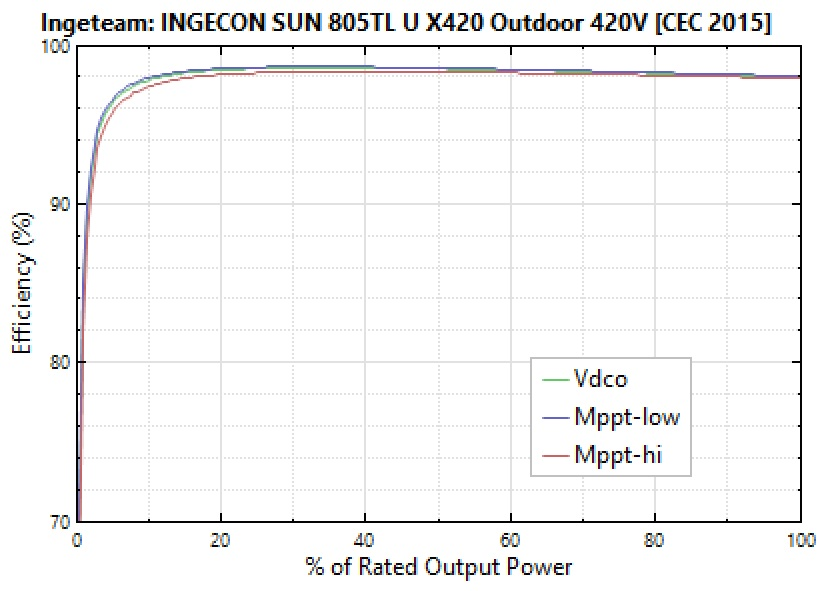
\includegraphics[width=0.75\linewidth]{FIG/InverterEfficiencyCurve}
\caption[Efficientcy characteristic of Ingecon Sun 805TL U X420 Outdoor.]{Efficientcy characteristic of Ingecon Sun 805TL U X420 Outdoor \cite{IngeteamINC.2015,NREL2015g}.}\label{InverterEfficiencyCurve}
\end{figure}
\begin{table}[htbp]  
  \centering
	\begin{tabular}{ p{6.0cm}  C{7.0cm}  C{1.5cm} } 
	\hline	
\textbf{Item} & \textbf{Value} & \textbf{Unit} \\ \hline \hline
Manufacturer  & Ingeteam Power Technology & - \\ 
Model & Ingecon Sun 805TL U X420 Outdoor & - \\ 
Type &  central inverter & - \\ \hline
\textbf{Input (dc)} &  &  \\ 
Maximum power & 821.39 & kW\textsubscript{dc} \\ 
Voltage range & 611-820 & V\textsubscript{dc} \\ 
Maximum voltage & 1~000 & V\textsubscript{dc} \\ 
Maximum current & 1~350 & A\textsubscript{dc} \\
Nominal voltage & 715.91 & V\textsubscript{dc} \\ \hline
\textbf{Output (ac)} &  &  \\ 
Maximum power & 805 & kW\textsubscript{ac} \\ 
Nominal voltage & 420 & V\textsubscript{ac} \\
Maximum current & 1.35 & A\textsubscript{ac} \\
Frequency & 50-60 & Hz \\
cos$\phi$ & 1 & -\\ \hline
Maximum efficiency & 98.33 & \\% 
European efficiency & 98.29 & \\% 
Power consumption in operation &1.25 & kW\textsubscript{dc} \\ 
Power consumption at night & 0.12 & kW\textsubscript{ac} \\ 
\hline
\end{tabular}
\caption[Inverter specifications of Ingecon Sun 805TL U X420 Outdoor.]{Inverter specifications of Ingecon Sun 805TL U X420 Outdoor \cite{IngeteamINC.2015,NREL2015g}.}\label{tbl: PVinverter}
\end{table}
\newpage\noindent
As mentioned before the PV system was design under similar condition that the Mulilo Sonnedix Prieska PV Project. There a dc/ac ratio of 1.15 is used \cite{Morse2014}. This power ratio compares the photovoltaic array power to the inverter capacity \cite{Woodcock2013}. For the simulated PV system the same ratio was assumed. So at 100 MW\textsubscript{ac} inverter output, a total module capacity of 115 MW\textsubscript{dc} is needed. From the discussed parameter and the PVM SAM calculates the resulting number of modules and inverters as well as other parameters on its own. These PV system parameter are summarized in Table~\ref{tbl: PVsystemdesign}.

\begin{table}[!b]  
  \centering
	\begin{tabular}{ p{4.5cm} C{1.0cm} C{1.2cm} C{1.2cm} C{1.2cm} C{1.2cm} C{1.2cm} C{1.2cm} } 
	\hline	
\textbf{Item} & \textbf{Unit} & \multicolumn{6}{c}{\textbf{Value}} \\ \hline \hline
Module azimuth & $\,^{\circ}$ &\multicolumn{6}{c}{0 (north)}\\
Module tilt & $\,^{\circ}$ & \multicolumn{6}{c}{28.4}\\
Modules per string& - & \multicolumn{6}{c}{21}\\
String open circuit voltage& V\textsubscript{oc} & \multicolumn{6}{c}{955.3}\\
String max. power rated voltage& V\textsubscript{mp} & \multicolumn{6}{c}{759.8}\\
Maximum dc-voltage& V\textsubscript{dc} & \multicolumn{6}{c}{1~000}\\
Aspired dc/ac-ratio & - &\multicolumn{6}{c}{1.15}\\
\hline
\textbf{PV multiple} & - & \textbf{1.0} & \textbf{1.8} & \textbf{2.0} & \textbf{2.2} & \textbf{2.4} & \textbf{2.6}\\ \hline 
Total inverter capacity & MW\textsubscript{ac} & 99.8 & 180.3 &199.6 & 219.8 & 239.9 & 260.0 \\
Total module capacity & MW\textsubscript{dc} & 115.0 & 207.0 & 230.0 &253.0 & 276.0 & 299.0 \\
Strings in parallel & - & 17~954 & 32~318 & 35~909 & 39~500 & 43~091 & 46~682 \\
Number of modules & - & 377~034 & 678~678& 754~089 & 829~500 & 904~911 & 980~322 \\
Number of inverter  & - & 124 & 224 & 248 & 273 & 298 & 323 \\
Total module area & ha & 73.1 & 131.7 & 146.3 & 160.9 & 175.6 & 190.1 \\
Total land area & ha & 244 & 439 & 488 & 536 & 585 & 634 \\
\hline
\end{tabular}
\caption[PV system design parameter.]{PV system design parameter.}\label{tbl: PVsystemdesign}
\end{table}

For the orientation of the simulated PV-modules the latitude of Upington was used as tilt angle (28.4$\,^{\circ}$) and the azimuth is 0$\,^{\circ}$, so directly facing north. The self-shading model was selected, without external shading parameter. Therefore 2 modules along the side of row and 10 along the bottom of row was selected. Therefrom a shading loss of 0.545~\% on the solar radiation incident on the subarray. Further assumed losses are soiling, mismatch, diodes and connections and wiring losses. The assumed soiling losses reduce the solar radiation incident on the subarray of about 5~\%. The assumed mismatch loss of about 2~\% is related to slight differences in performance of individual modules in the array. Voltage drops across blocking diodes and electrical connections leads to a assumed diodes and connections loss of 0.5~\%. There are also assumed resistive losses of 2~\% in wiring on the dc-side and 1~\% wiring loss between the inverter and the grid connection point on the ac-side of the system. All PV system loss parameter coming from a IEEE photovoltaics specialists conference paper about performance parameters for grid-connected PV systems \cite{Marion2005}.
\subsubsection{Electrical energy storage (EES)}
The electrical energy storage is adapted though the system as it is shown in Figure~\ref{PV_model_config} on Page~\pageref{PV_model_config}. The EES basically consists out of two parts - the power conversions system (PCS) and the storage unit - as it is shown in Figure~\ref{TCC_EES} on Page~\pageref{TCC_EES}. For the simulation in SAM the PCS was simplified to the conversion efficiency. The AC to DC conversion efficiency was assumed with 99~\% as well as the DC to AC efficiency. Nevertheless for the LCOE calculation it is still relevant to define the performance of the PCS. As it is shown in Table~\ref{tbl: PVsystemdesign} the inverter capacity range is between 240 and \SI{320}{MW}\textsubscript{ac} for the simulation cases with adapted storage. The maximum scheduled load from Section~\ref{Overall simulated configuration} is \SI{100}{MW}. So depending from the PV inverter capacity the PCS capacity needs to variate as well to collect the  PV-overproduction. For the calculation of the LCOE it was assumed that the PCS needs to collects the inverter capacity minus the \SI{100}{MW} daily base load.



As mentioned before the storage unit consists out of a Li-Ion battery, more precisely a using a Nickel Cobalt Aluminum ($LiNiCoAlO_2$  or NCA) cathode. This battery excels through a less expensive cathode material with improved safety characteristics and high specific energy \cite{NREL2015a}. The voltage characteristics of these battery for the simulation are shown in Figure~\ref{EES_VoltageDischarge}. The NCA battery is inter alia installed in the Tesla Model S and X \cite{Nykvist2015} which uses currently Panasonic cells and will also be installed in Teslas Power Wall system \cite{Shahan2015}. The performance and lifetime of the NCA batteries depending on how they are used. Tesla names the lifetime of 5~000 cycles without mentioning the assumed depth of discharge (DOD) \cite{Shahan2015}.

\begin{figure}[!htbp]  
\centering
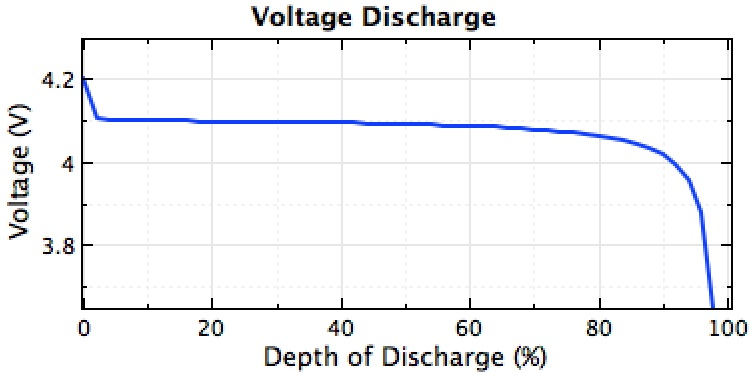
\includegraphics[width=0.6\linewidth]{FIG/EES_VoltageDischarge}
\caption[Voltage proparties of NCA Li-Ion battery.]{Voltage proparties of NCA Li-Ion battery..}\label{EES_VoltageDischarge}
\end{figure}



The DOD is the amount of capacity in the battery that is usable by the system. For electric vehicles (EV) the DOD is set between 80-95~\% at the "top" end of the battery and 10-20~\% at the "bottom" end \cite{Warner2014}. The state of charge (SOC) is an expression of the present battery capacity as a percentage of maximum capacity and is the inverse of the DOD. It must be noted, that the nominal capacity of a battery is not the effective usable capacity of a battery and depends on the DOD. Also the DOD effects the cycle life of the batteries. The higher the DOD, the lower the cycle life. In other words, the lower the SOC, the longer the cycle life. \cite{MitElectricVehilceTeam2008}



SAM visualizes the decreasing capacity of the battery over the number of cycles with capacity fades as it is shown in Figure~\ref{CapacityFade} for the NCA. The figure shows the characteristic for 20~\% and 80~\% DOD. As mentioned above the graph shows the higher decreasing of the effective capacity at higher DOD. The performance data behind this graph is coming from \cite{Dahn2011} and correspond with other tests \cite{Read2009}.
\begin{figure}[bhtp]  
\centering
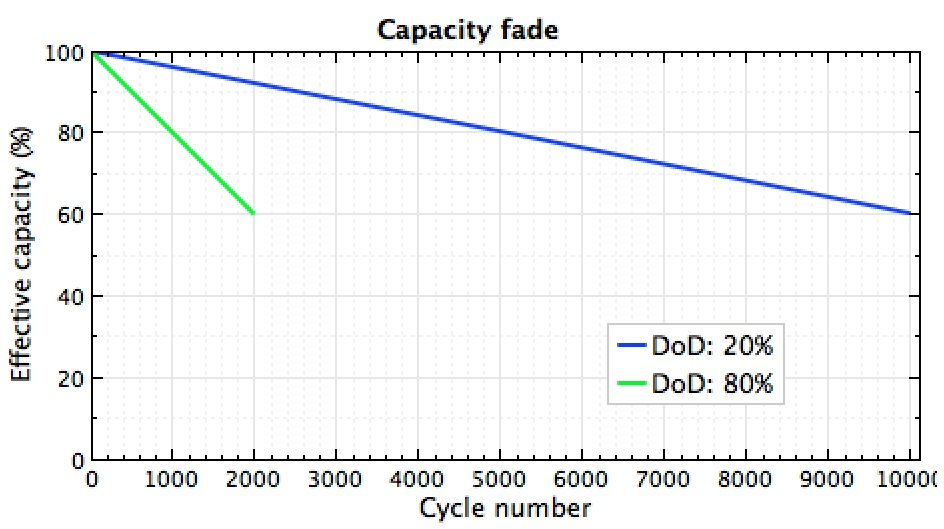
\includegraphics[width=0.75\linewidth]{FIG/CapacityFade}
\caption[Capacity fade of Nickel Cobalt Aluminum Lithium-Ion battery.]{Capacity fade of Nickel Cobalt Aluminum Lithium-Ion battery.}\label{CapacityFade}
\end{figure}

It must be noted, that the cycle lifetime is not only affected by the DOD but also by other conditions such as temperature and humidity \cite{MitElectricVehilceTeam2008}. SAM designs the cycle lifetime for the batteries at a constant room temperature of 20\si{\celsius} therefore the storage room needs to be conditioned. Also the charging and discharging of the battery results losses in form of heat which needs to get led away. The cooling demand of the EES system is not included in the simulation, but must be actually significant. \cite{Diorio2015} 



The system was designed for a lifetime of 25 years. Therefore also the EES is designed for this period. For the simulation a amount of 365 cycles per year was assumed. So the NCA was designed for 9~125 cycles whiteout using a battery bank replacement. SAM also can analyses the cycle lifetime of the batteries. This analyses showed that the NCA battery reaches this cycle lifetime with a DOD of 50~\%. But under this conditions the effective capacity of the battery is nearly 0~\% after 25 years. As it is shown in Figure~\ref{CapacityFade} the effective capacity of the NCA battery decreases almost lineal with the cycle number. There are two opportunities to reduce the loss to the effective capacity increasing over the lifetime of the system. First is a battery bank replacement after a specified schedule or loss of effective capacity to a specified amount and second is to use a lower DOD which leads also to a lower effective usable capacity of the battery, so a higher nominal capacity of the battery would be necessary.



Further is to note that Li-Ion batteries has a expiry period \cite{Jossen2006}. Tesla gives a warranty of 10 years of the batteries \cite{Shahan2015} so it can be expected, that the expiry period is close to these warranty. So also for the simulation an battery bank replacement is indispensable.



The for a long lifetime an average SOC of 30-70~\% is recommended for Li-Ion batteries \cite{Jossen2006}. Consequently the SOC was set to a maximum of 30~\% and a minimum of 70~\% for the simulation. So a total DOD of 40~\% which signified 40~\% of the nominal battery capacity was assumed as usable. In order to have high storage availability over the total system lifetime it was assumed that the battery bank will replaced at a effective capacity loss of 20~\%. This is also advised for EES in electronic consumer devices \cite{Spotnitz2003}. Resulting from this assumptions the cycle lifetime of the cells in the battery bank is 2~500 cycles. Therefore the battery bank needs to be replaced after 6-\SI{7}{years}. So the battery bank needs to be replaced three times in the total lifetime of the system. 



Table~\ref{tbl: EESsystemdesign} summarizes results of the discussed parameter for the simulation. The adapted voltage level for this large-scale EES application from \SI{820}{V}\textsubscript{dc}\ per string is coming from \cite{Leuthold2014}. The remaining values results from the above discussed parameter or are adapted from the SAM library \cite{Diorio2015}. 
\begin{table}[!htbp]  
  \centering
	\begin{tabular}{ p{5.0cm} C{1.0cm} C{1.2cm} C{1.2cm} C{1.2cm} C{1.2cm} C{1.2cm} } 
	\hline	
\textbf{Item} & \textbf{Unit} & \multicolumn{5}{c}{\textbf{Value}} \\ \hline \hline
Chemistry & - & \multicolumn{5}{c}{Lithium ion: nickel cobalt aluminum oxide} \\
Cell nominal voltage & V\textsubscript{dc} &\multicolumn{5}{c}{3.6}\\
Internal resistance & Ohm &\multicolumn{5}{c}{0.1}\\
Fully charged cell voltage & V\textsubscript{dc} &\multicolumn{5}{c}{4.2}\\
Exponential zone cell voltage & V\textsubscript{dc} &\multicolumn{5}{c}{4.1}\\
Nominal zone cell voltage & V\textsubscript{dc} &\multicolumn{5}{c}{3.6}\\
Nominal bank voltage & V\textsubscript{dc} &\multicolumn{5}{c}{820}\\
Cells in in series& - &\multicolumn{5}{c}{228}\\
Cell capacity & Ah &\multicolumn{5}{c}{55}\\
C-rate of discharge curve & - &\multicolumn{5}{c}{0.2}\\
Maximum C-rate charge & per/h &\multicolumn{5}{c}{1}\\
Maximum C-rate discharge & per/h &\multicolumn{5}{c}{1}\\
Total DOD& \% &\multicolumn{5}{c}{20}\\
\hline
\textbf{Storage capacity at \SI{100}{MW} output} & \textbf{h} & \textbf{4} & \textbf{5} & \textbf{6} & \textbf{7} & \textbf{8} \\ \hline 
Effective capacity & MWh & 400 & 500 & 600 & 700 & 800 \\
Nominal capacity & MWh & 1~000 & 1~250 & 1~500 & 1~750 & 2~000\\
Cells & $\times 10^6$ & 5.1 & 6.3 & 7.6 & 8.8 & 10.1\\
\hline
\end{tabular}
\caption[EES system design parameter.]{EES system design parameter.}\label{tbl: EESsystemdesign}
\end{table}
\pagebreak
\subsubsection{Financial parameter}
The financial parameter for the LCOE calculation are composed in Table~\ref{tbl: PVFinance}. As mentioned before was the LCOE calculation for this simulation made separately in Microfoft Excel using a simplified method which is documented in Appendix~\ref{ChapterLCOE} on Page \pageref{ChapterLCOE}. As for the other systems is the PV power plant designed for a lifetime of \SI{25}{years}. 

The specific large-scale PV system costs in South Africa  amount to \SI{1.285}{USD/W}\textsubscript{p} (\SI{14.5}{ZAR/W}\textsubscript{p} using \SI{11.286}{USD/ZAR} average in 2014 \cite{IRS2015}) which leads from an in 2014 actually built PV system \cite{Terblanche2015}. These specific costs are close to utility-scale PV systems in Europe with specific investments of \SI{1}{EUR/W}\textsubscript{p} \cite{FraunhoferISE2013}, corresponding to \SI{1.33}{USD/W}\textsubscript{p} (using the average exchange rate in 2014 of \SI{1.33}{USD/EUR}  \cite{StatistaGmbH2015}).

The LCOE was calculated with different interest rates and O\&M costs for the PV power plant and the EES system. The real interest rate for the PV power plant was amused with 2.8~\% \cite{FraunhoferISE2013} and the annual O\&M costs are 1~\%  of the PV investment costs \cite{IEA2014a}. A degradation of 1~\% per year of the annual energy output was assumed for the ageing phenomena of the PV cells \cite{Tidball2010}.

The storage costs are calculates from three  parts. The costs for the PCS, the battery bank and the replacement costs of the battery bank during the lifetime of the system.

The costs of the PCS of \SI{615}{USD/kW} (\SI{463}{EUR/kW} using the average exchange rate in 2014 of 1.33 USD/EUR \cite{StatistaGmbH2015}) was taken over from a study toward comparative life cycle cost analysis of EES \cite{Zakeri2015}. This is the average value of  a wide cost range (250-600€/kW) of PCS for Li-Ion EES systems.

For the storage part of the EES a highly optimistic value of \SI{300}{USD/kWh} was assumed from \cite{Nykvist2015}. The average storage part cost for Li-Ion EES in other studies is \SI{914}{USD/kWh} \cite{Zakeri2015}.

For the replacement costs of the an other highly optimistic value of \SI{150}{USD/kWh} was assumed. The cost for the replacement of the storage in \cite{Zakeri2015} are approximately the half of the storage costs. This costs was also assumed with a look to Figure~\ref{CostofLi-ion} on Page~\pageref{CostofLi-ion}.

The assumed EES battery bank replacements during the lifetime was described in this Chapter already.

The annual O\&M costs of \SI{9.18}{USD/kW} was also a adaption from \cite{Zakeri2015} as well as the real interest rate of 8.0~\%.

As before for the other solar power plants also for the PV system was land purchase costs of 3~000USD/ha \cite{Cassell2012} assumed.
\pagebreak
\begin{table}[!h]  
  \centering
	\begin{tabular}{  p{5.4cm} C{1.5cm} C{1.5cm}  C{1.7cm}  C{4.0cm} } 
	\hline	
\textbf{Item} & \textbf{Symbol}& \textbf{Value} & \textbf{Unit} & \textbf{Source}\\ \hline \hline
Lifetime &$n$ & 25 & years & \cite{FraunhoferISE2013} \\ \hline
Solar modules & $c_{sm}$&0.481 & USD/W\textsubscript{p} & \cite{Terblanche2015}\\ 
Structural &$c_{st}$ &0.138 & USD/W\textsubscript{p} & \cite{Terblanche2015} \\ 
Electrical parts &$c_{ep}$ &0.116 & USD/W\textsubscript{p} & \cite{Terblanche2015} \\ 
Inverters&$c_{inv}$ &0.117 & USD/W\textsubscript{p} & \cite{Terblanche2015} \\ 
Engineering and labour costs & $c_{elc}$ & 0.242 & USD/W\textsubscript{p} & \cite{Terblanche2015} \\ 
Security and infrastructure & $c_{si}$& 0.091 & USD/W\textsubscript{p} & \cite{Terblanche2015} \\ 
Transport and logistics & $c_{tl}$& 0.067 & USD/W\textsubscript{p} & \cite{Terblanche2015}\\ 
Sub-Station & $c_{ss}$ & 0.071 & USD/W\textsubscript{p} &\cite{Terblanche2015} \\ \hline
Total PV system costs & $c_{PV}$ & 1.285 &  USD/W\textsubscript{p} &\cite{Terblanche2015} \\ 
Annual degradation factor &$f_{degrad}$ & 1 & \% & \cite{Tidball2010}\\ 
Annual PV O\&M costs factor &$f_{O\&M,PV}$ & 1 & \% & \cite{IEA2014a}\\
Interest rate of PV & $i_{PV}$& 2.8 & \% & \cite{FraunhoferISE2013} \\ 
Annual insurance costs & $f_{ins,PV}$ & 0.5 & \% & \cite{InternationalFinanceCorporation2015}\\ \hline
EES PCS costs & $c_{EES,PCS}$ & 615 & USD/kW & \cite{Zakeri2015} \\ 
EES battery bank costs & $c_{EES,BBC}$ &300 & USD/kWh & \cite{Nykvist2015} \\ 
EES battery bank replacement costs & $c_{EES,BBRC}$ & 150 & USD/kWh & \cite{Zakeri2015} \\ 
Assumed EES battery bank replacements during lifetime & $n_{BBR}$ & 3 & - & - \\ 
Annual EES O\&M costs & $c_{O\&M,EES}$ & 9.18 & USD/kW & \cite{Zakeri2015}\\
Interest rate of EES & $i_{EES}$& 8.0 & \% & \cite{Zakeri2015} \\
Annual insurance costs& $f_{ins,EES}$ & 0.5 & \% & \cite{Cutter2014}\\ \hline
Land purchase &$c_{LP}$ & 3~000.00 & USD/ha & \cite{Cassell2012} \\ 
\hline
\end{tabular}
\caption[Finacial input parameter for PV-simulation in SAM.]{Finacial input parameter for PV-simulation in SAM.}\label{tbl: PVFinance}
\end{table}
\pagebreak
\subsection{Simulation results of PV power plant}
In this section the results of the simulated PV system and there belonging LCOE results are described and analyzed. First the PV system without EES and then the results of the PV system with adapted EES. The goal of these Section is to find the suitable PV power plant design configuration to reach a covering of 90~\% of the prescribed load which having the lowest belonging LCOE result.
\subsubsection{PV power plant without storage}
As it was described before at the beginning of Section~\ref{section PV system}, the PV system was also simulated without using an EES system. These PV system was designed for a maximum power output of \SI{99.8}{MW}\textsubscript{ac} and \SI{115.0}{MW}\textsubscript{dc} as it is defined in Table~\ref{tbl: PVsystemdesign}. It must be noted, that the following results are simulated for the first year of the PV system so for the performance results contains no degradation which is to be expected during the full lifetime. For the LCOE calculation a degradation factor was assumed as it was described in the previous section. 

Figure \ref{PVwithoutEESanual} visualizes the resulting annually load covering behavior. It can be seen, that the system can't cover the prescribed load at all. As it is usually for a solar powered system without storage the energy production standstill during the night time. The here shown annual average PV system power output covers about 32.9~\% of the prescribed load in the first year of the system. So the simulated PV system had a annual energy production during the first year of about \SI{233.69}{GWh}.

\begin{figure}[htbp]  
\centering
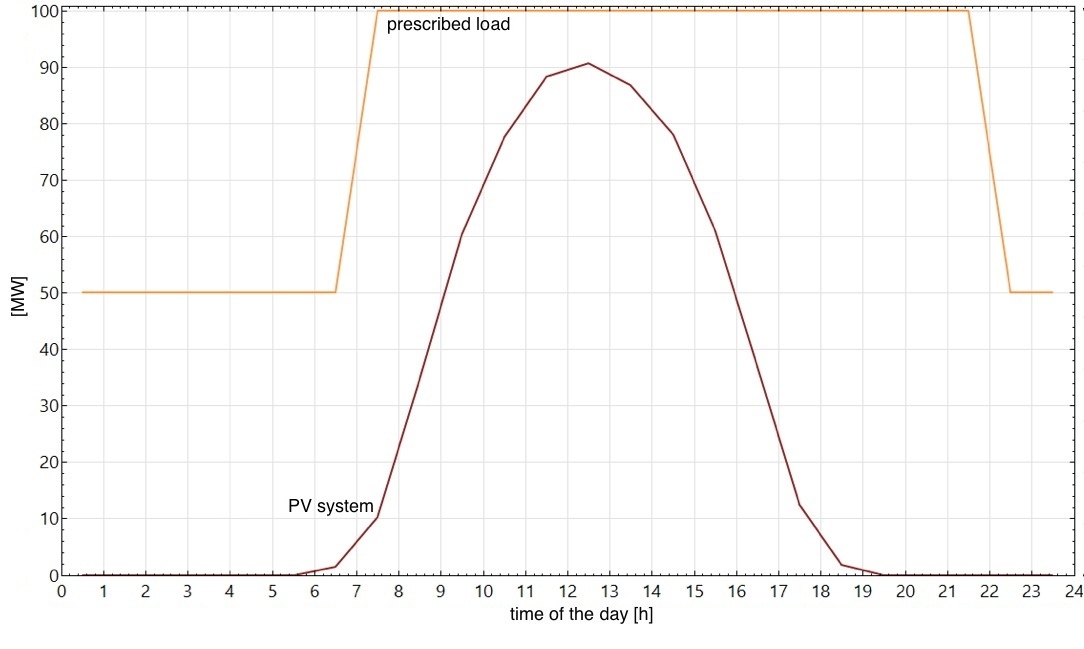
\includegraphics[width=0.8\linewidth]{FIG/PVwithoutEESanual}
\caption[Annual average profile of the simulated PV power plant without EES.]{Annual average profile of the simulated PV power plant without EES.}\label{PVwithoutEESanual}
\end{figure}
The simulation results of the energy output behavior in Figure~\ref{PVwithoutEES} shows that there is a small differences of the daily peak system power output between winter and summer time even though the GHI peak during the summer time is about twice that high then the winter peak. This leads from the irradiation angle of the sunlight and the fixed module tilt angle. However, the shorter sunshine duration reduces the daily energy output anyways. Especially appreciable is the situation at the noon of the 27. December. There the PV field produces more than the inverter can process because they reached there max output power of \SI{99.8}{\mega\watt}\textsubscript{ac}. At this day the PV system produces \SI{767}{\mega\watt\hour}, comparing this to the energy production at the 27. June (\SI{548}{\mega\watt\hour}) the difference in energy production between a summer and a winter day is just about \SI{29}{\percent}.

\begin{figure}[!htbp]
        \centering                
        \begin{subfigure}[b]{0.5\textwidth}
                \centering
                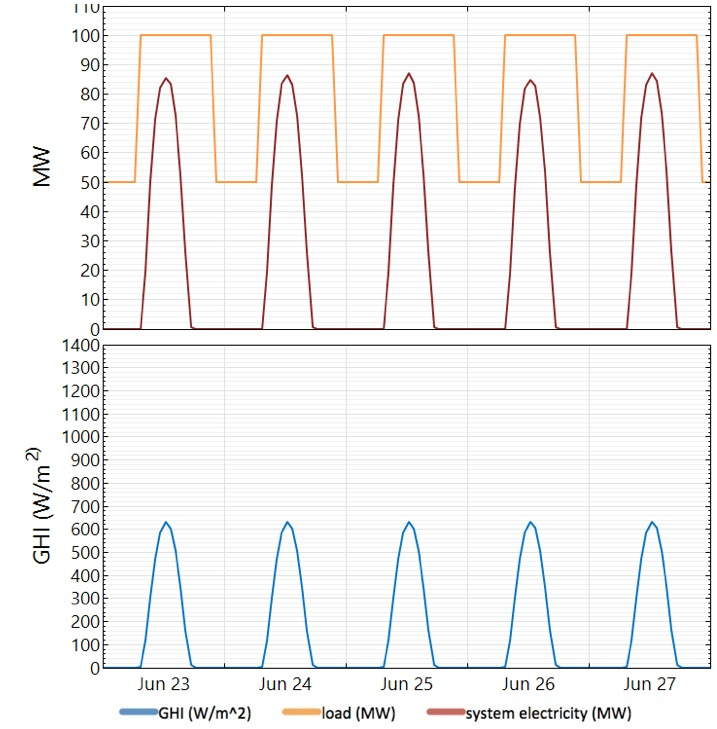
\includegraphics[width=1\textwidth]{FIG/PVwithoutEESwinter}
                \caption{Power output behavior short after winter solstice (23. to 27. June).}\label{PVwithoutEESwinter}
        \end{subfigure}%
        ~
        \begin{subfigure}[b]{0.5\textwidth}
                \centering
                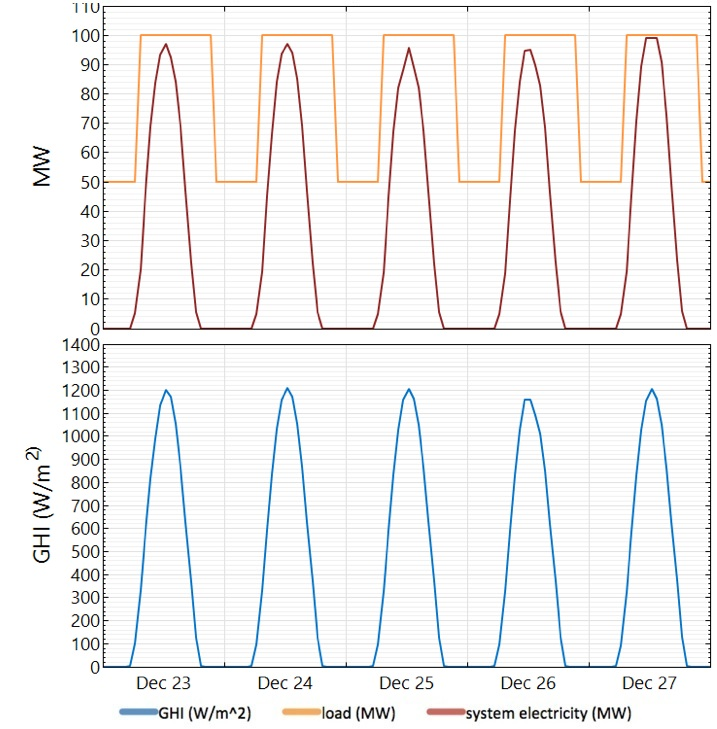
\includegraphics[width=1\textwidth]{FIG/PVwithoutEESsummer}
                \caption{Power output behavior short after summer solstice (23. to 27. December).}\label{PVwithoutEESsummer}
        \end{subfigure}
        \caption[Power output behavior of PV system.]{Power output behavior of PV system.}\label{PVwithoutEES}
\end{figure}
The LCOE was calculated taking into account of 1~\% annual degradation of the PV modules and under use of the remaining values from Table~\ref{tbl: PVFinance}. The LCOE was calculated using a the in Appendix~\ref{ChapterLCOE} documented method and results \SI{50.81}{USD/MWh}. Table~\ref{tbl: PVwithoutEESresult} summarizes the results of the PV system without adapted EES.
\begin{table}[htbp]  
  \centering
	\begin{tabular}{  p{3.0cm}  C{3.0cm}  C{3.0cm} } 
	\hline	
\textbf{Item} & \textbf{Value} & \textbf{Unit} \\ \hline \hline
First year energy & 233.69 & GWh \\ 
Load covering &  32.9 & \% \\ 
LCOE result & 50.81 & USD/MWh \\
\hline
\end{tabular}
\caption[Summary of the results of the simulated PV system without EES.]{Summary of the results of the simulated PV system without EES.}\label{tbl: PVwithoutEESresult}
\end{table}
\pagebreak
\subsubsection{Load curve covering}
The PV system was also simulated with the adapted EES system as it was described before in Section~\ref{section PV system}. In order to find a suitable size of the PV system and for the adapted EES, there was 25 different configurations simulated as they are described in Table~\ref{tbl: PV_OverallConfig}. The lowest defined configuration was simulated using a PVM of 2.0 and a \SI{4}{h} of EES. The highest simulation configuration was defined with a PVM of 2.8 and a EES capacity for \SI{8}{h} at \SI{100}{MW} output. In the following the simulation results of these configurations are delineated  representative for the remaining 23 configurations in between. 

The simulation results are based on the first year energy output of the designed PV power plants and don't includes degradation of the PV system or the adapted EES system. 

The result of the simulation for the both selected configurations are present in the annual average load profile in Figure~\ref{PV_annual_profil}. The simulation result shows that the highest configuration can cover the load almost completely during the simulated first year and just has appreciable shortfalls of covering in the morning hours. Considering the the load curve behavior from \SI{10}{am} to \SI{4}{pm} it can be noticed, that the predicted load is covered over the whole year in that time span. Compared to that covers the lowest PV power plant configuration much less of the predicted load curve. The  annual average load profile shows that during the night the system coming to standstill from 12 pm to 5 am over the full year. Nevertheless, the PV power plant can cover the prescribed load completely during the midday at any time of the year. The remaining  annual average load profile simulation results can be found in Appendix~\ref{all_load_profile}.

\begin{figure}[htbp]  
\centering
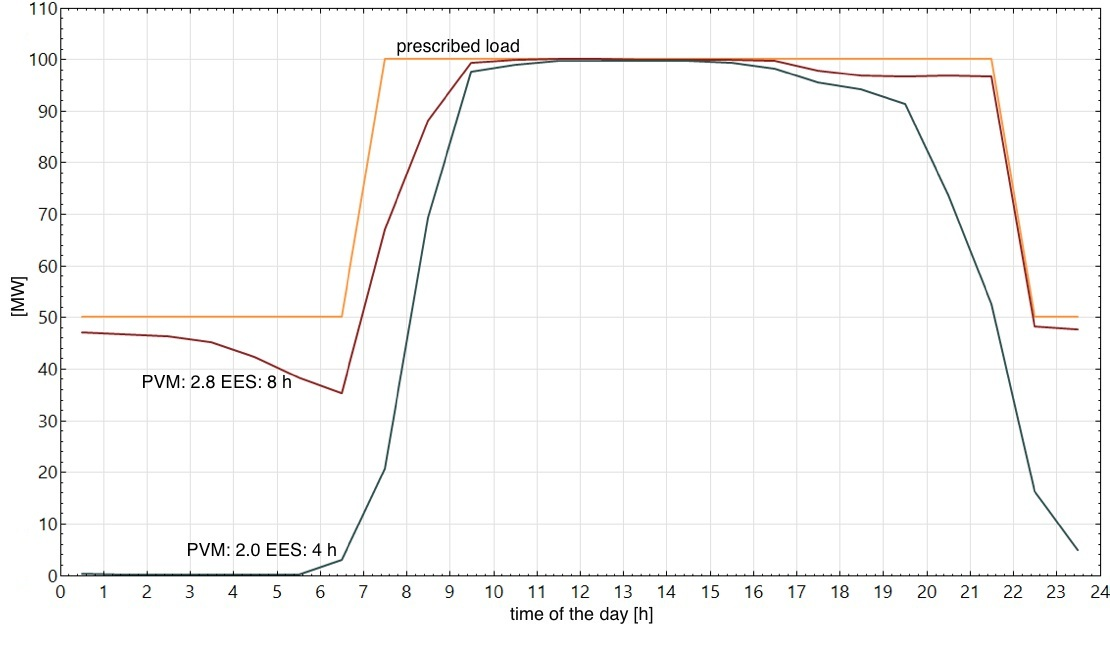
\includegraphics[width=0.8\linewidth]{FIG/PV_annual_profil}
\caption[Annual average load profile of selected PV power plant configurations.]{Annual average load profile of selected PV power plant configurations.}\label{PV_annual_profil}
\end{figure}
The covering of the prescribed load during the day results mainly from the PV system, which also loads with there surplus power production the EES. During the night the EES taken over the covering of the load till it reaches the fixed bottom limit of the SOC. If the EES is fully loaded and the PV system is still producing more electricity than the prescribed load needs the surplus power is not going in to the load curve covering calculation as well as into the LCOE calculation as it was defined in Section~\ref{Overall simulated configuration}. 

\begin{figure}[!bhtp]  
\centering
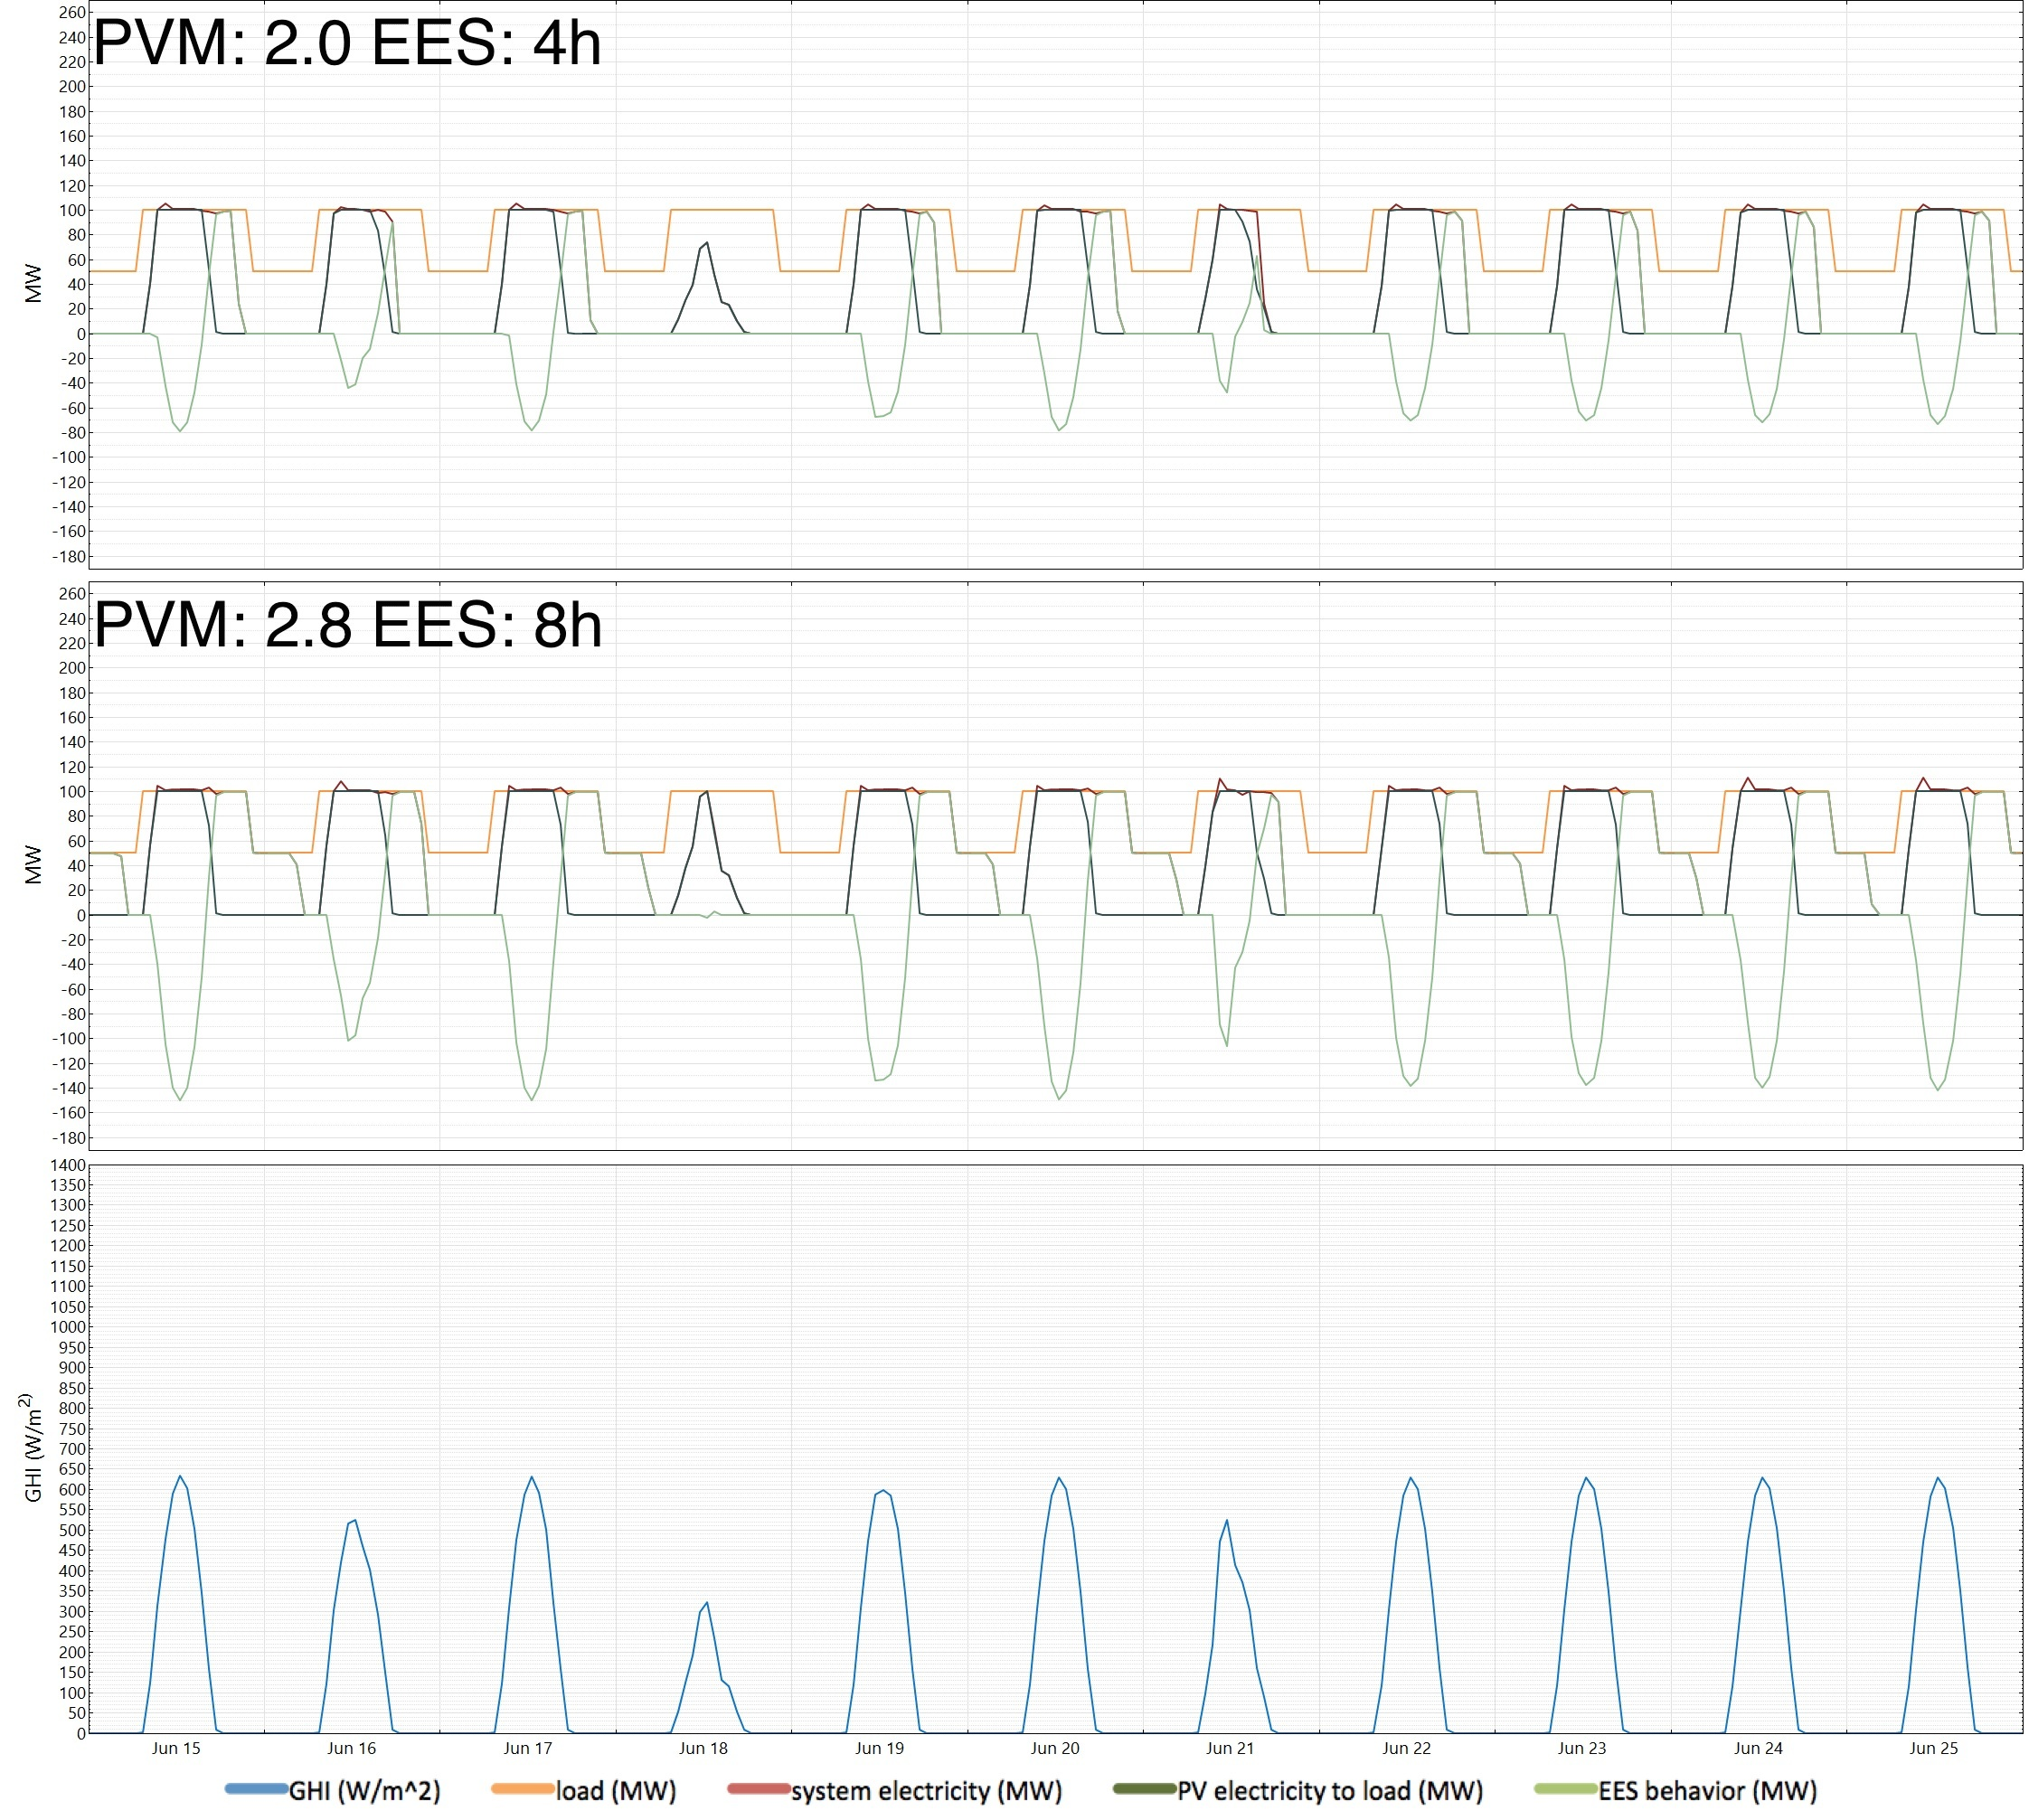
\includegraphics[width=1\linewidth]{FIG/PV_winter_load}
\caption[PV system with adapted EES load profile during the time of winter solstice.]{PV system with adapted EES load profile during the time of winter solstice (15. June - 25. June).}\label{PV_winter_load}
\end{figure}
The behavior of the power output of the selected simulated PV power plants and there power flow is shown in Figure~\ref{PV_winter_load} for the time with the lowest irradiance values. During the time of the winter solstice the value of GHI reaches just about \SI{630}{\watt\per\square\metre} in peak. The graph shows the behavior of the EES during the days and as it was described above the PV system first covers the prescribed load and then charges the EES with there surplus power. In the time span of the 22. to the 25. of June are the irradiance values of GHI during the days almost perfect. Nevertheless, both PV power plant configurations can't produce power without coming to standstill. The configuration with a PVM of 2.0 and \SI{4}{h} of EES stops covering the prescribed load before this steps down to the night reduction. But the PV power plant configuration with a PVM of 2.8 and \SI{8}{h} of EES covering the load till in the early morning hours. When comparing the value of the EES charging power it is obviously that there higher charging power peaks at a higher PVM configuration a the lower. 

During the winter times captures the EES the whole electricity power from the simulated PV systems, but this is not always the situation during the summer times. Figure~\ref{PV_summer_load} shows the load profile during the longest days of the year for the two selected configurations of the simulated PV power plants. The GHI rises up to \SI{1210}{\watt\per\square\metre} in peak at the portrayed time span.

\begin{figure}[htbp]
\centering
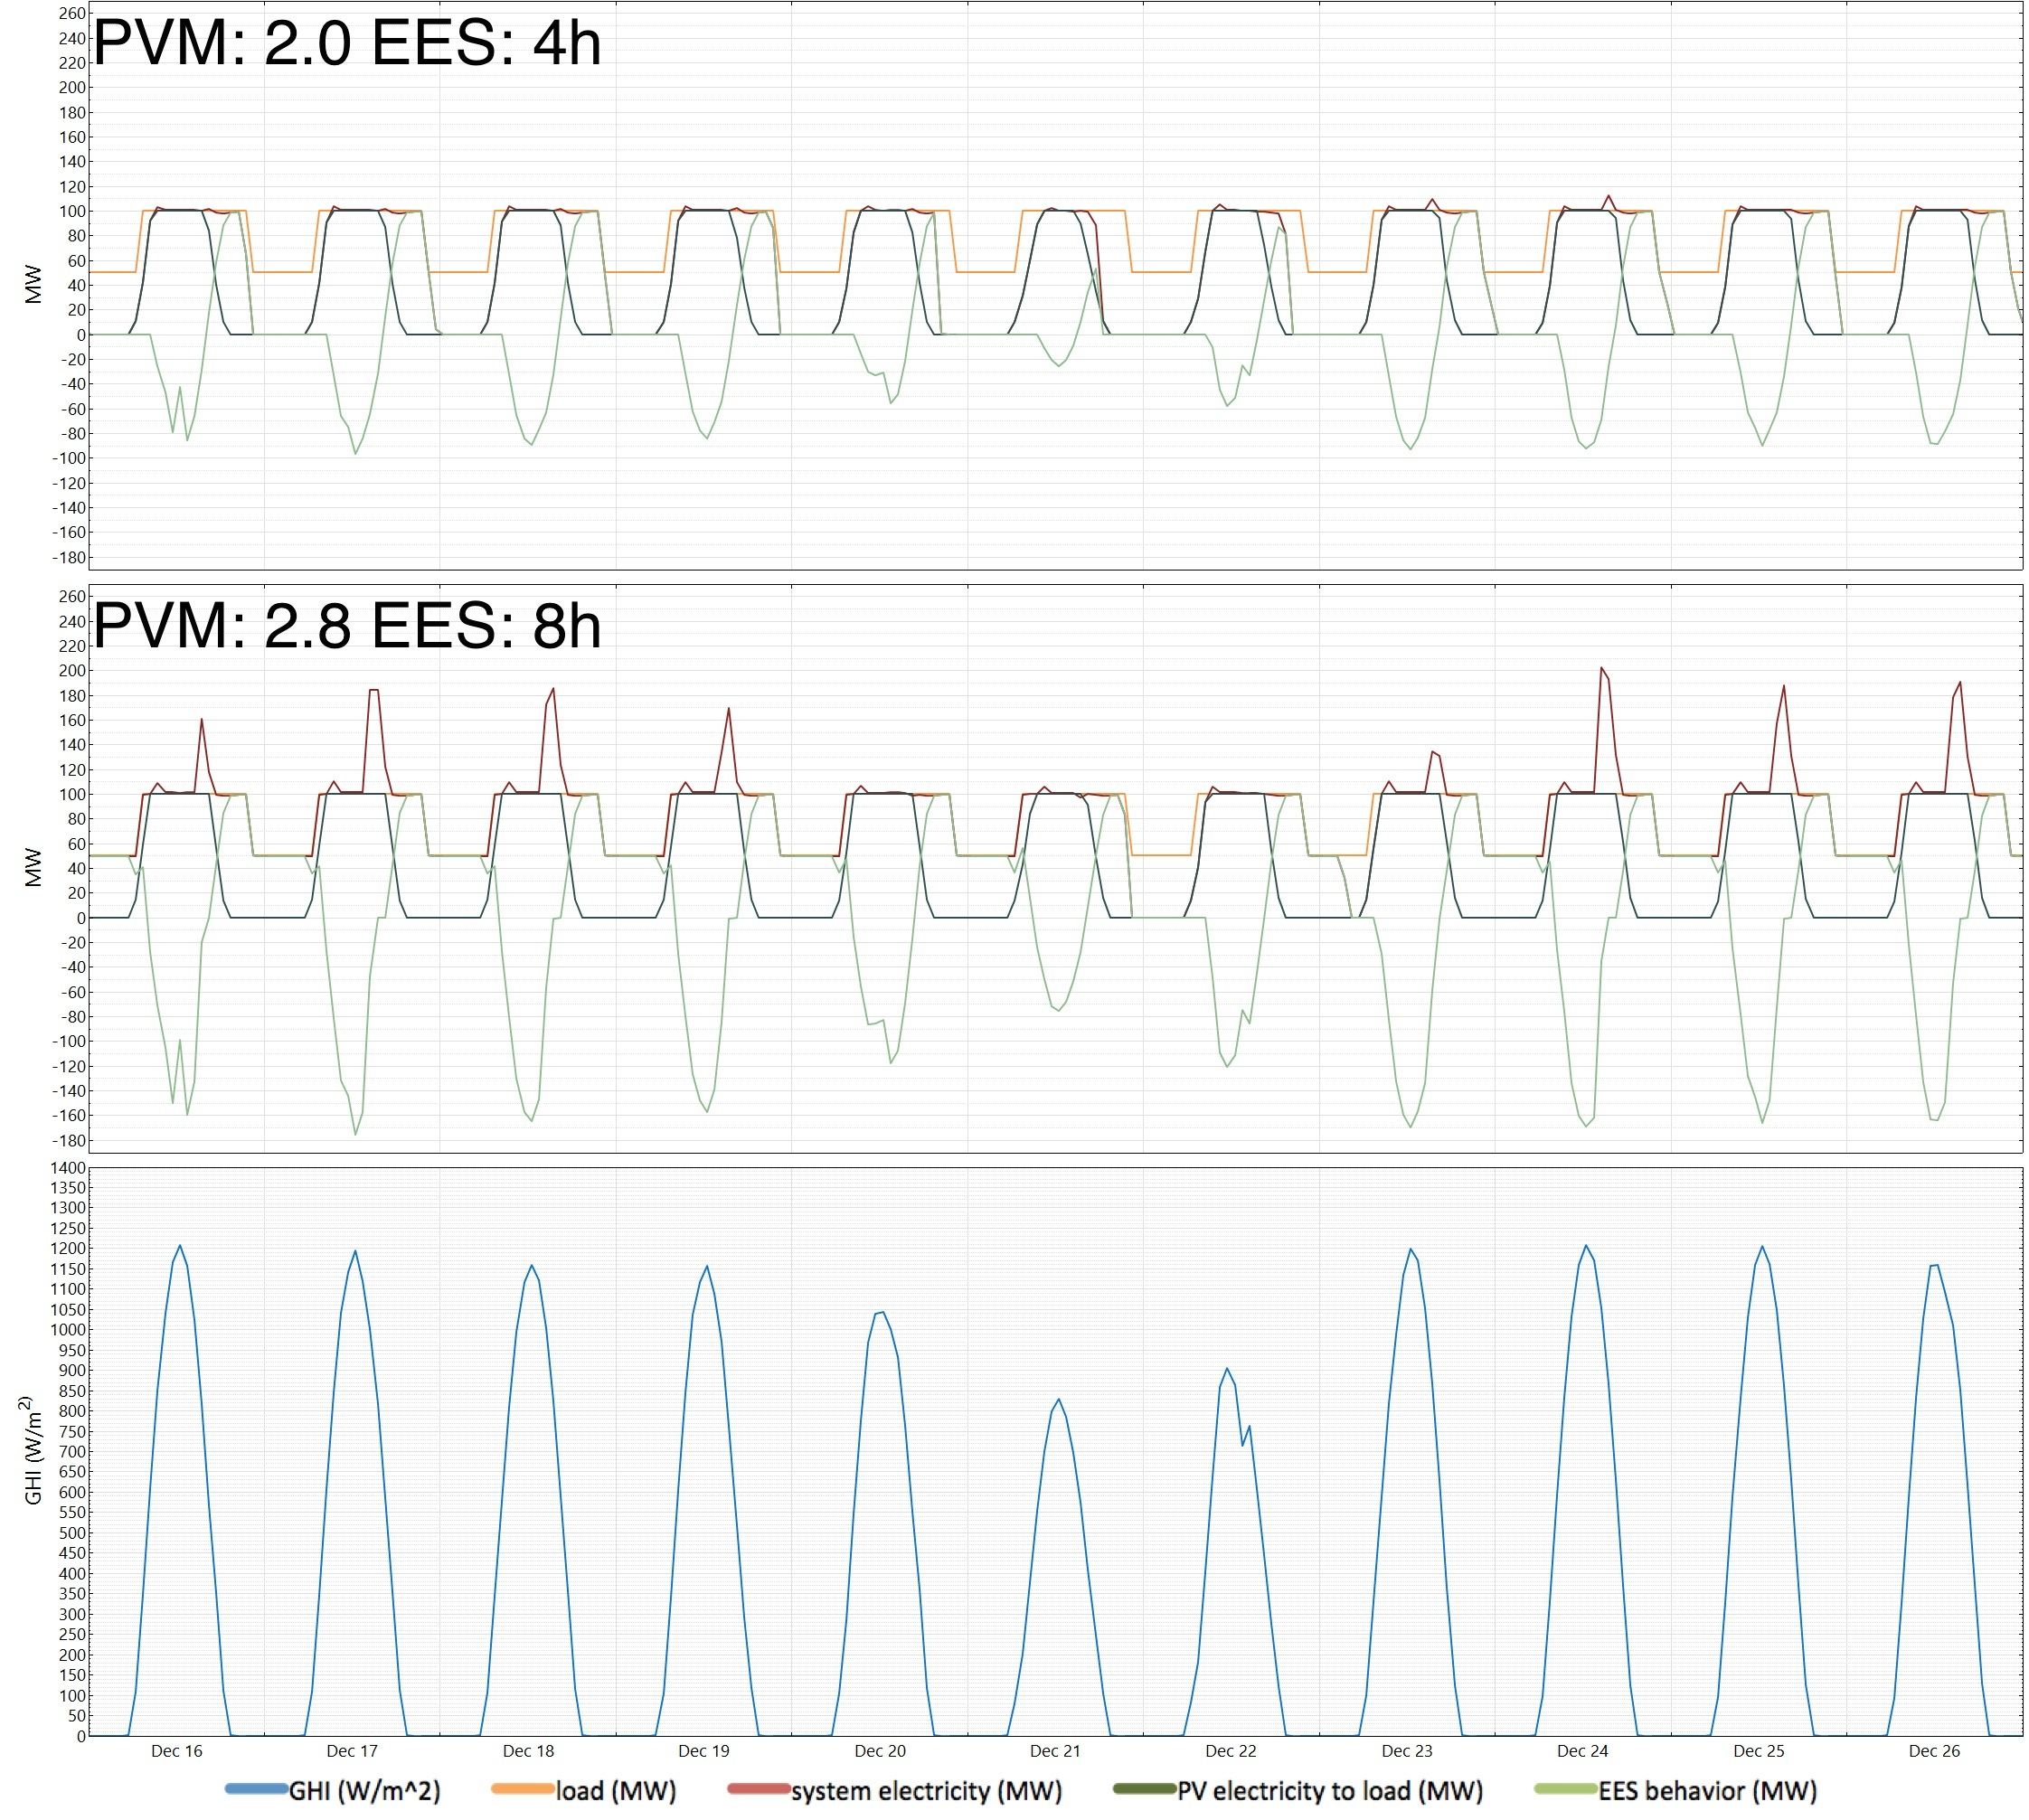
\includegraphics[width=1\linewidth]{FIG/PV_summer_load}
\caption[PV system with adapted EES load profile during the time of summer solstice.]{PV system with adapted EES load profile during the time of summer solstice (16. December - 26. December).}\label{PV_summer_load}
\end{figure}
The graph shows that the lowest PV power plant configuration can't cover the prescribed load during the night. The by the system provided power coming to stand still when the load got reduced for the night reduction at latest. Therefore the electricity production standstill during the night in the annual average load profile (Figure~\ref{PV_annual_profil}) as well. In comparison to that covers the highest PV power plant configuration almost the full prescribed load. Just during the following night times of days with lower irradiance (21. \& 22. December) comes the systems electricity output to standstill. Considering the system electricity output more precise, it offers high overproduction peaks which are the above mentioned situations where the storage got full charged and the PV system produces more power than the load requests.  

This surplus output depends on the ratio between the PV and EES system. The behavior of the ratio is shown in Figure~\ref{PV_energy_output}, which describes the share of the PV power plants energy output in the first year. The chart shows that the share of surplus energy rises with a higher PVM and decreases by larger EES capacity.

\begin{figure}[htbp]  
\centering
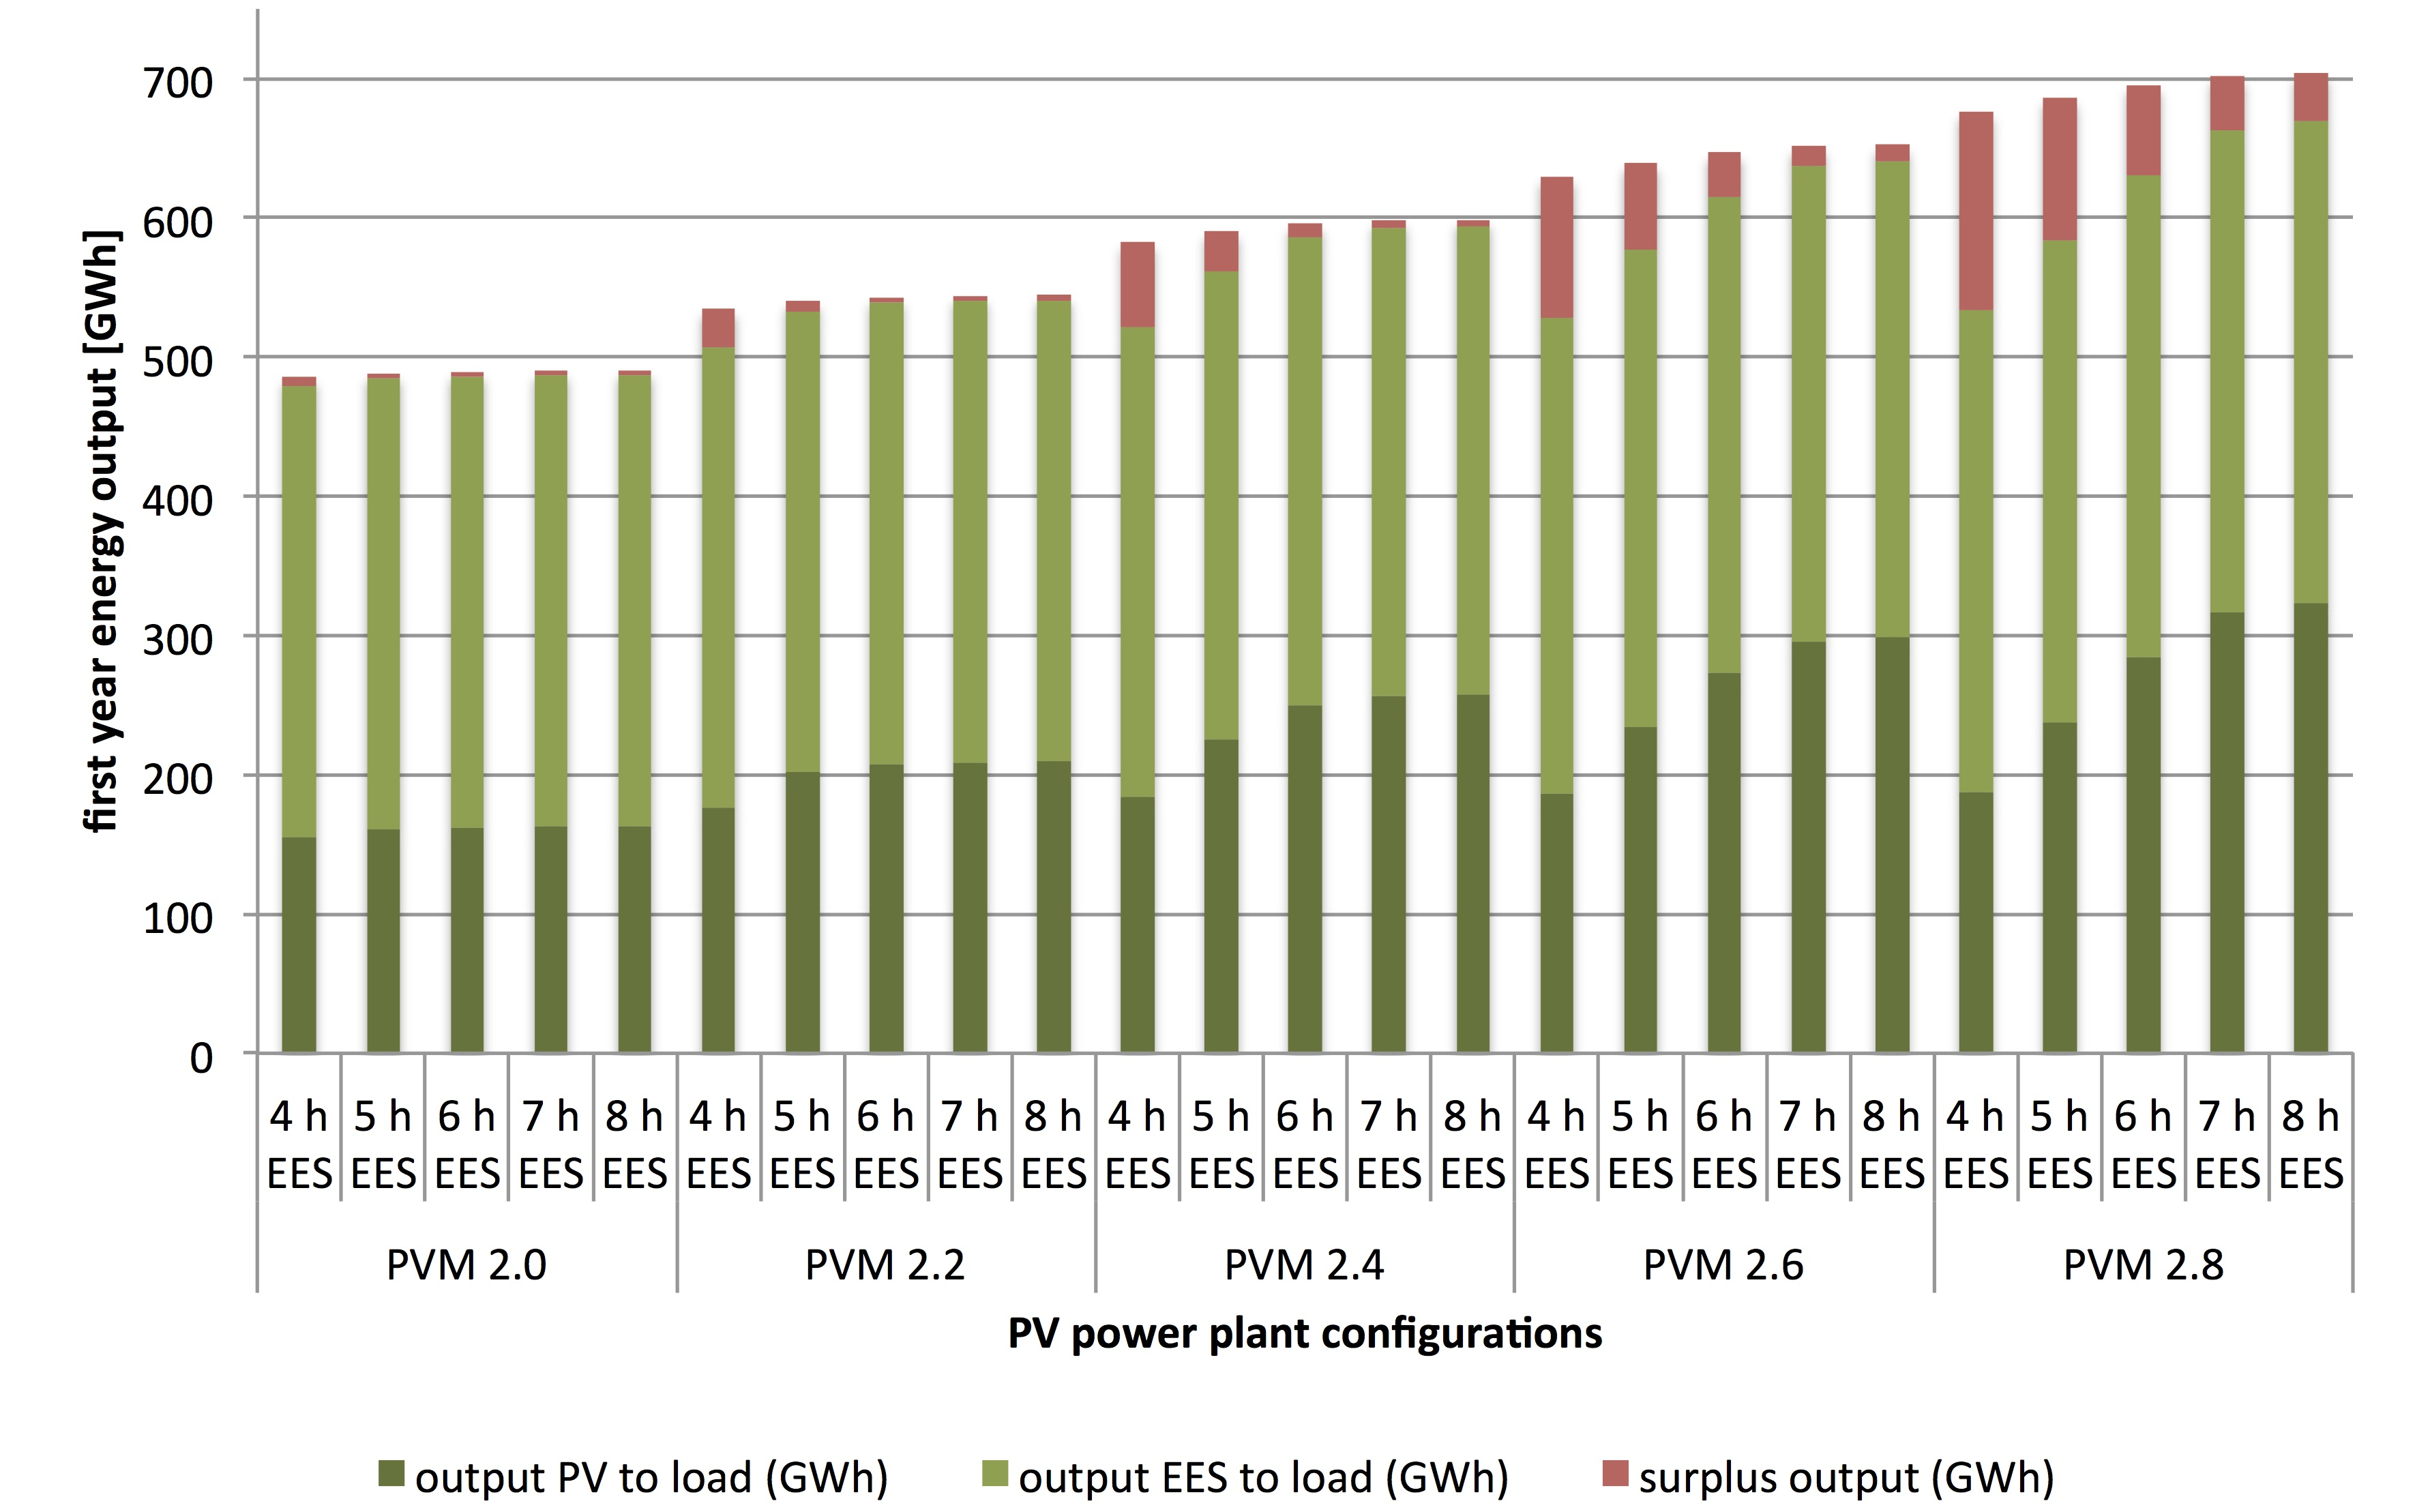
\includegraphics[width=1\linewidth]{FIG/PV_energy_output}
\caption[Share of energy output of all simulated PV power plants with adapted EES.]{Share of energy output of all simulated PV power plants with adapted EES.}\label{PV_energy_output}
\end{figure}
The Figure also gives an idea of the amount of the energy output of the simulated PV power plants for covering the prescribed load. The lowest simulated configuration produces an energy output of about \SI{479.54}{GWh} in the first year which covers the prescribed load. The total sum of the annual prescribed load is \SI{711.75}{GWh}. Consequently, the lowest configuration of the simulated PV power plants covers 67.4~\% of the prescribed load in the first year. The share of the surplus output is 1.2~\% of the total generated energy. The energy output of the highest simulated configuration has a share of a surplus output of about 4.9~\% and produces an load covering energy output of about \SI{669.44}{GWh} in the first year. This output covers 94.1~\% of the prescribed load.

The from the energy output derived load curve covering results of the simulated PV power plant are shown in Figure~\ref{PV_LCCF}. At a PVM of 2.0 the size of the variations of EES don't have a big influence to the load curve covering. With the rising PVM the significance of the EES capacity gains as well. The forced target to covering 90~\% of the prescribed load is reached with the EES configuration 7 and \SI{8}{h} from a PVM of 2.6 on. The configuration PVM 2.6 with \SI{7}{h} of EES reaches actually just about 89.58~\% but reaching the 90~\% by round up. 70~\% load covering is reached by all EEs capacities and besides of the \SI{4}{h} EES configuration also all simulated EES variants reaching the covering of 80~\% of the prescribed load. 

\begin{figure}[htbp]  
\centering
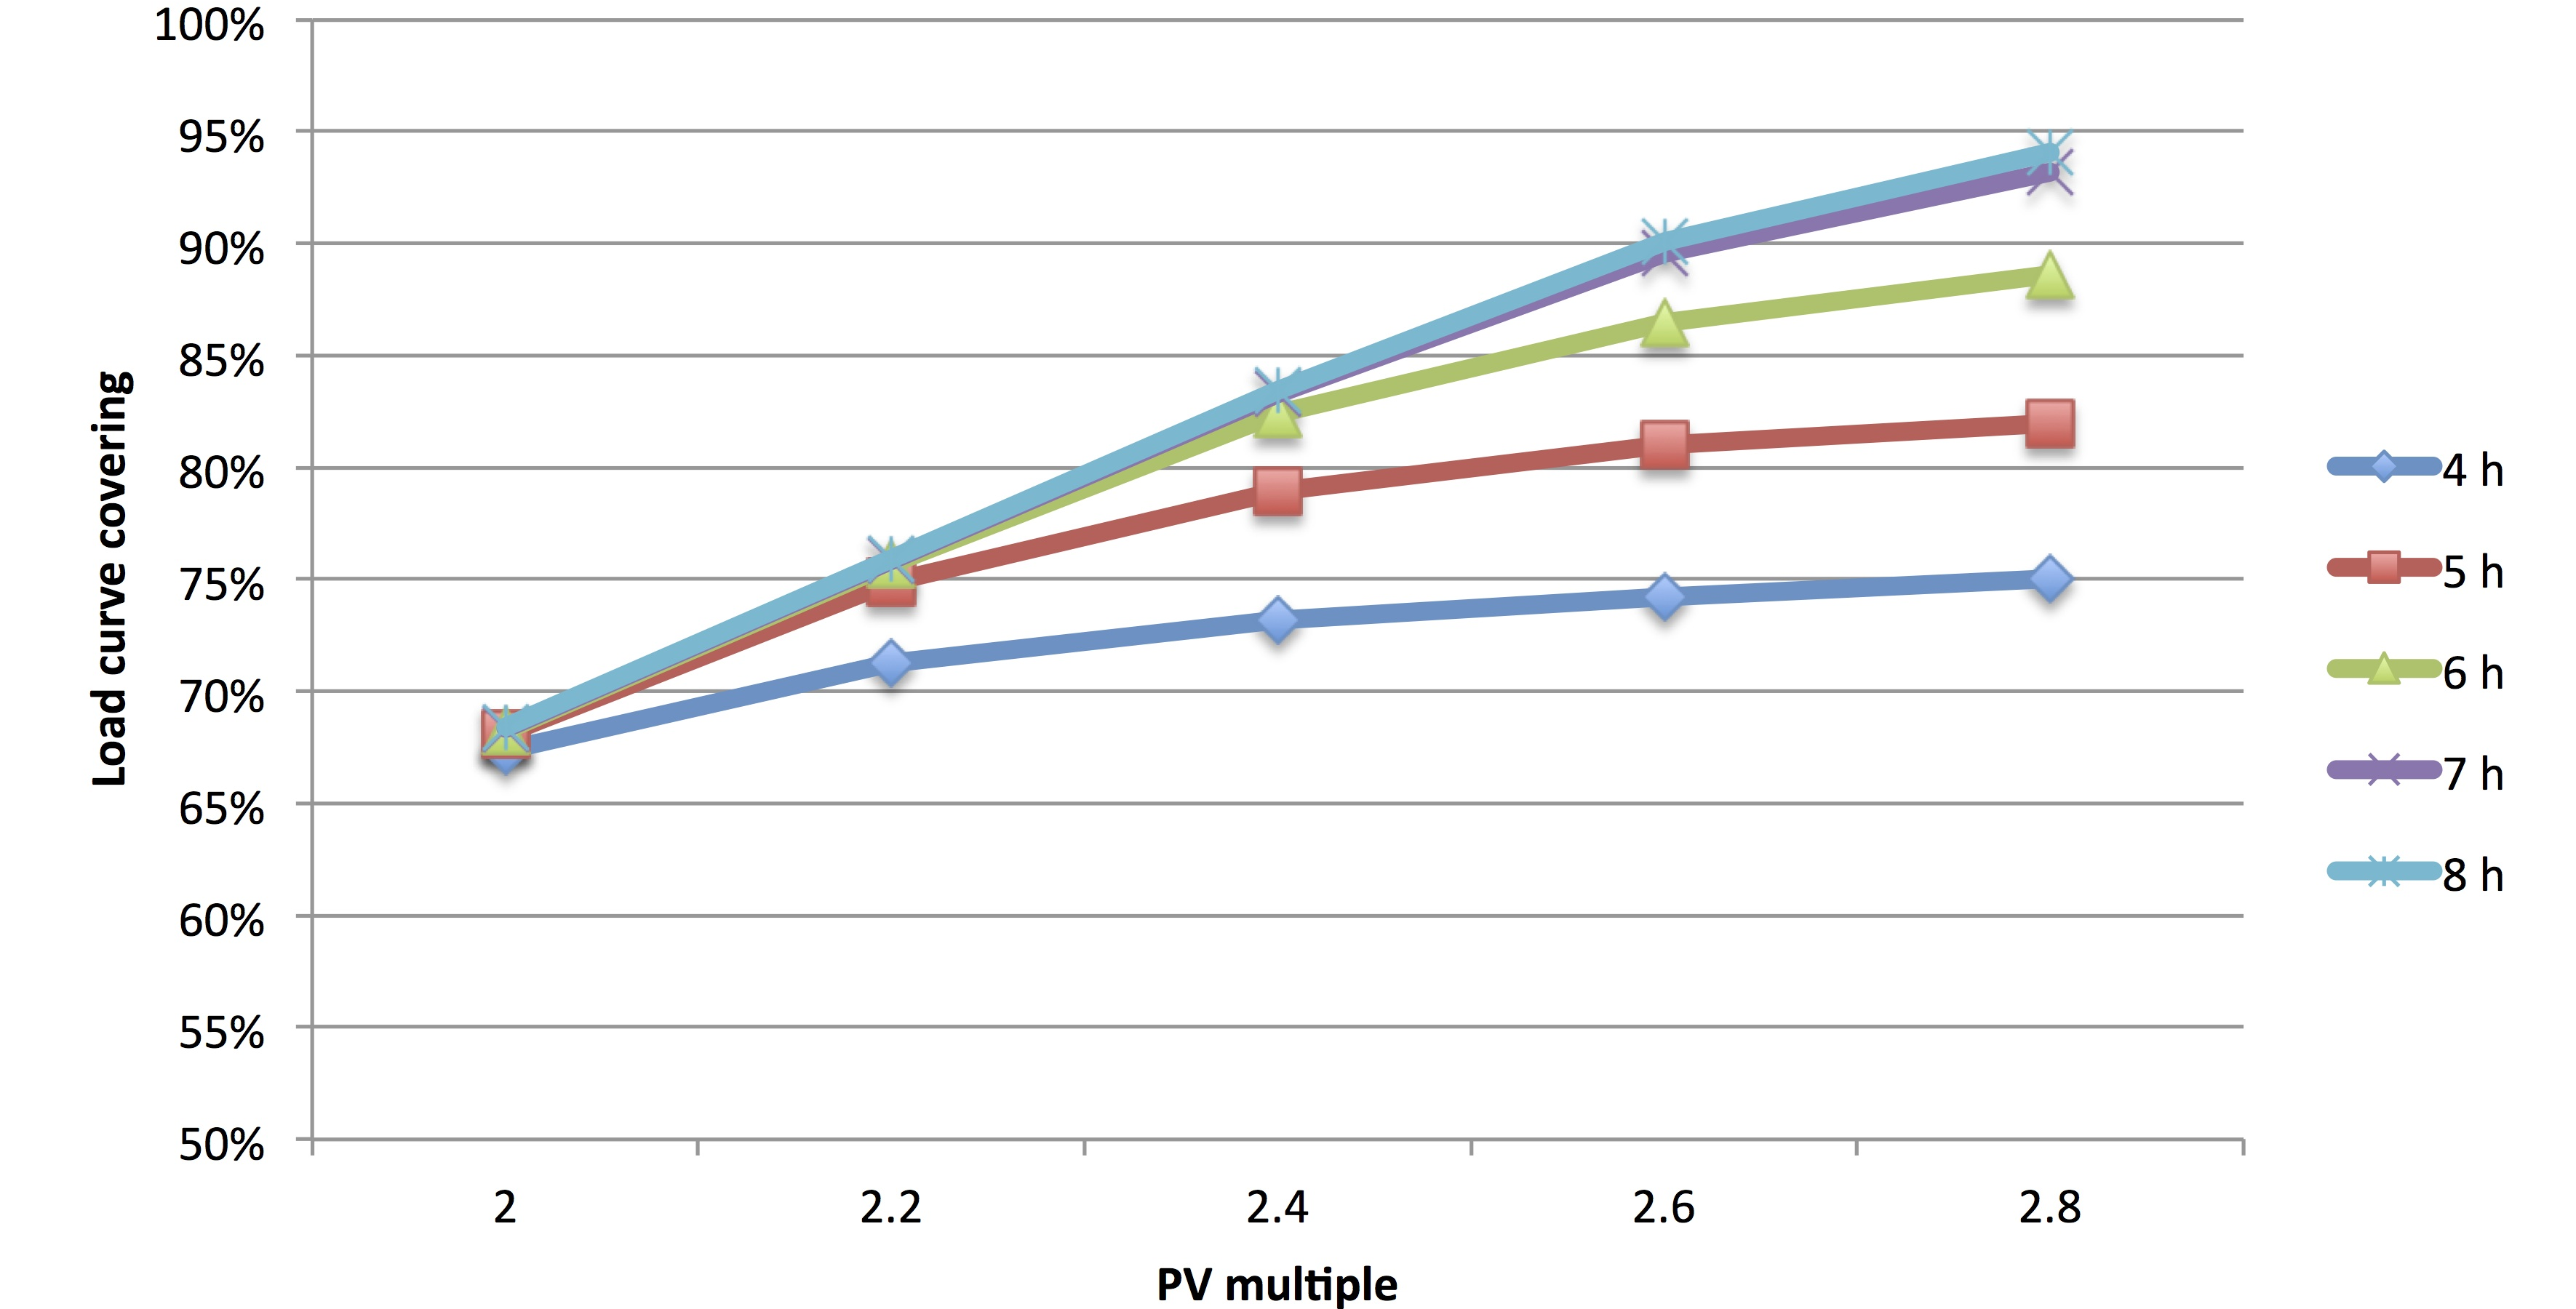
\includegraphics[width=1\linewidth]{FIG/PV_LCCF}
\caption[Load curve covering result of simulated PV systems with adapted EES.]{Load curve covering result of simulated PV systems with adapted EES.}\label{PV_LCCF}
\end{figure}
\pagebreak
\subsubsection{Levelized costs of electricity}
The LCOE was calculated by using the finacial input parameter from Table~\ref{tbl: PVFinance} and a simplified method which is documented in Appendix~\ref{ChapterLCOE} on Page \pageref{ChapterLCOE}. It must be noted, that the calculation is based on the simulation result for the first year PV power plant results under consulting of a degradation factor for the PV system, but not for the EES. The results of the LCOE claculation for the simulated PV power plant configurations can be seen in Figure~\ref{PV_LCOE}. 

The lowest LCOE result of \SI{251.83}{USD/MWh} is reached at a PVM of 2.2 and the lowest EES configuration and is marginal lower than  \SI{252.42}{USD/MWh} at a PVM of 2.4 with the same EES configuration. Generally must be said that there are no overlaps of LCOE lines in this chart and the spacing leads from the EES system costs.

\begin{figure}[htbp]  
\centering
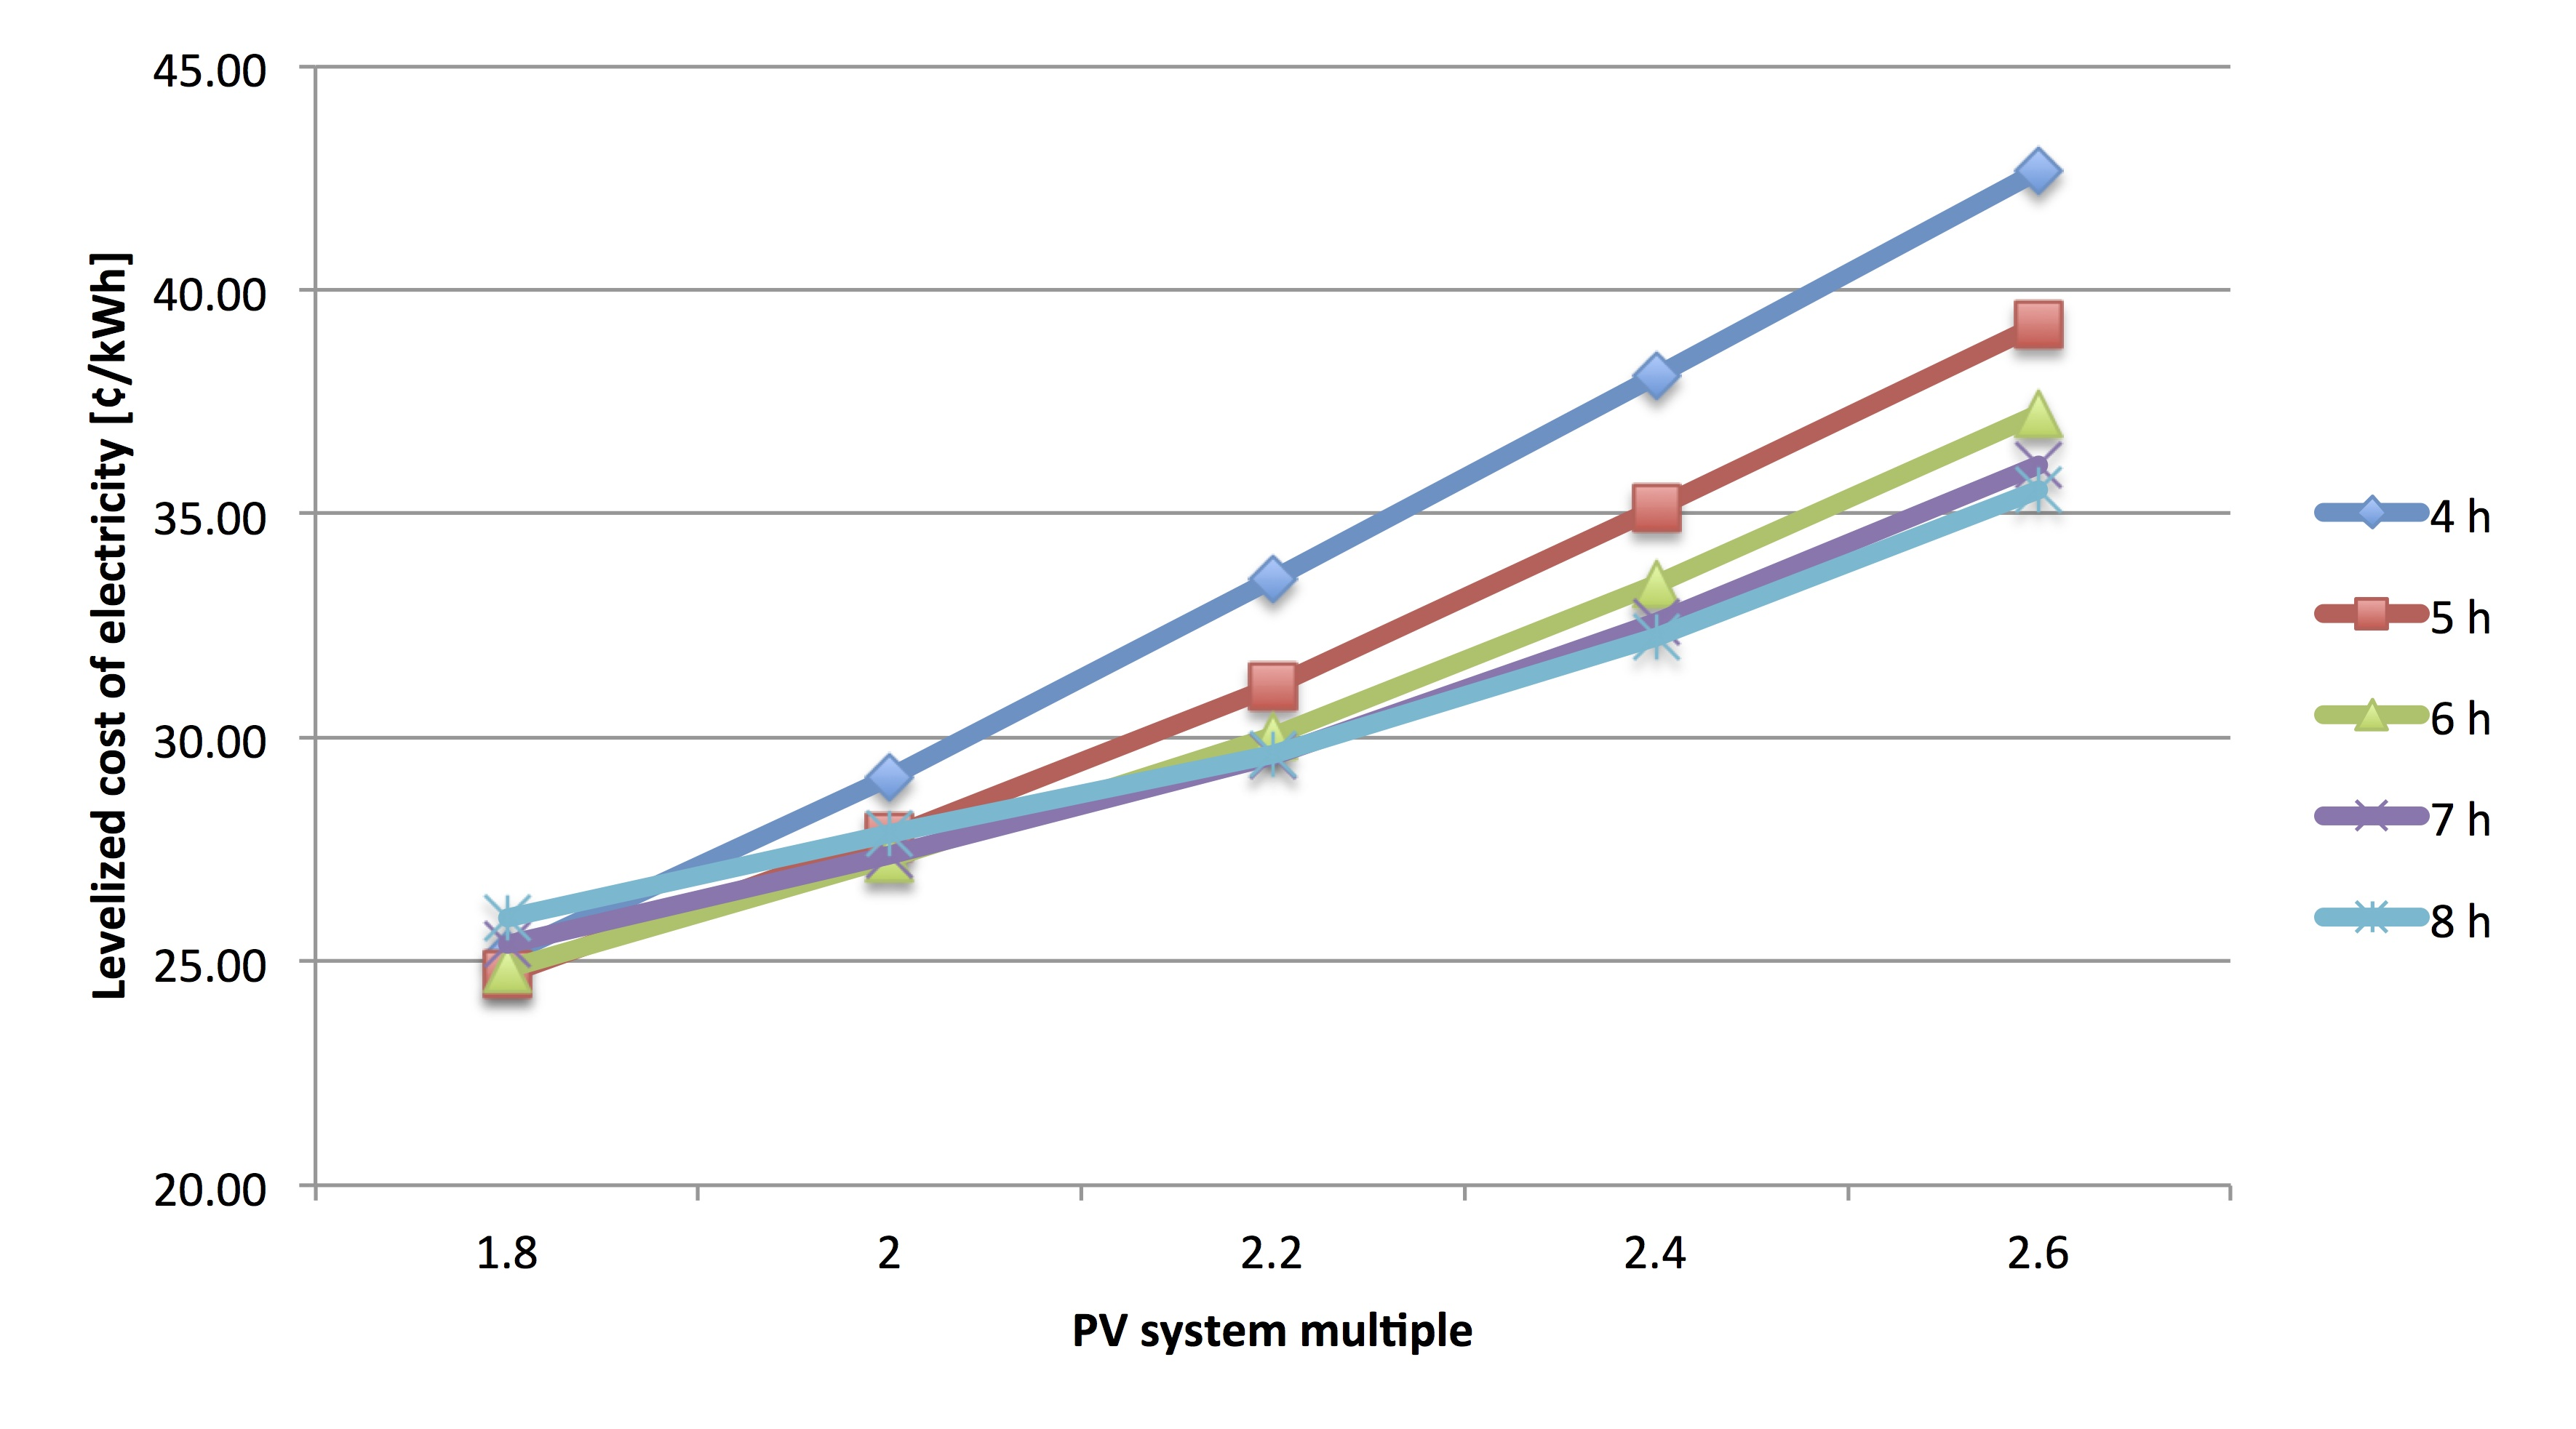
\includegraphics[width=1\linewidth]{FIG/PV_LCOE}
\caption[LCOE calculation results for PV systems with adapted EES simulation.]{LCOE calculation results for PV systems with adapted EES simulation.}\label{PV_LCOE}
\end{figure}
The EES systems costs share makes the main part of the LCOE cost of the simulated PV power plants with an adapted EES. The break-down of the LCOE is shown for the lowest and highest configuration in Figure~\ref{SMPV_LCOE_BreakDown}. This chart clarify the big impact of the EES cost. At the lowest configuration 81~\% of the LCOE are traced to the EES and at the highest about 86~\%. The other results showed that the range of the EES is between 76\% and 89~\% of the calculated LCOE's.

\begin{figure}[!htbp]
        \centering                
        \begin{subfigure}[b]{0.5\textwidth}
                \centering
                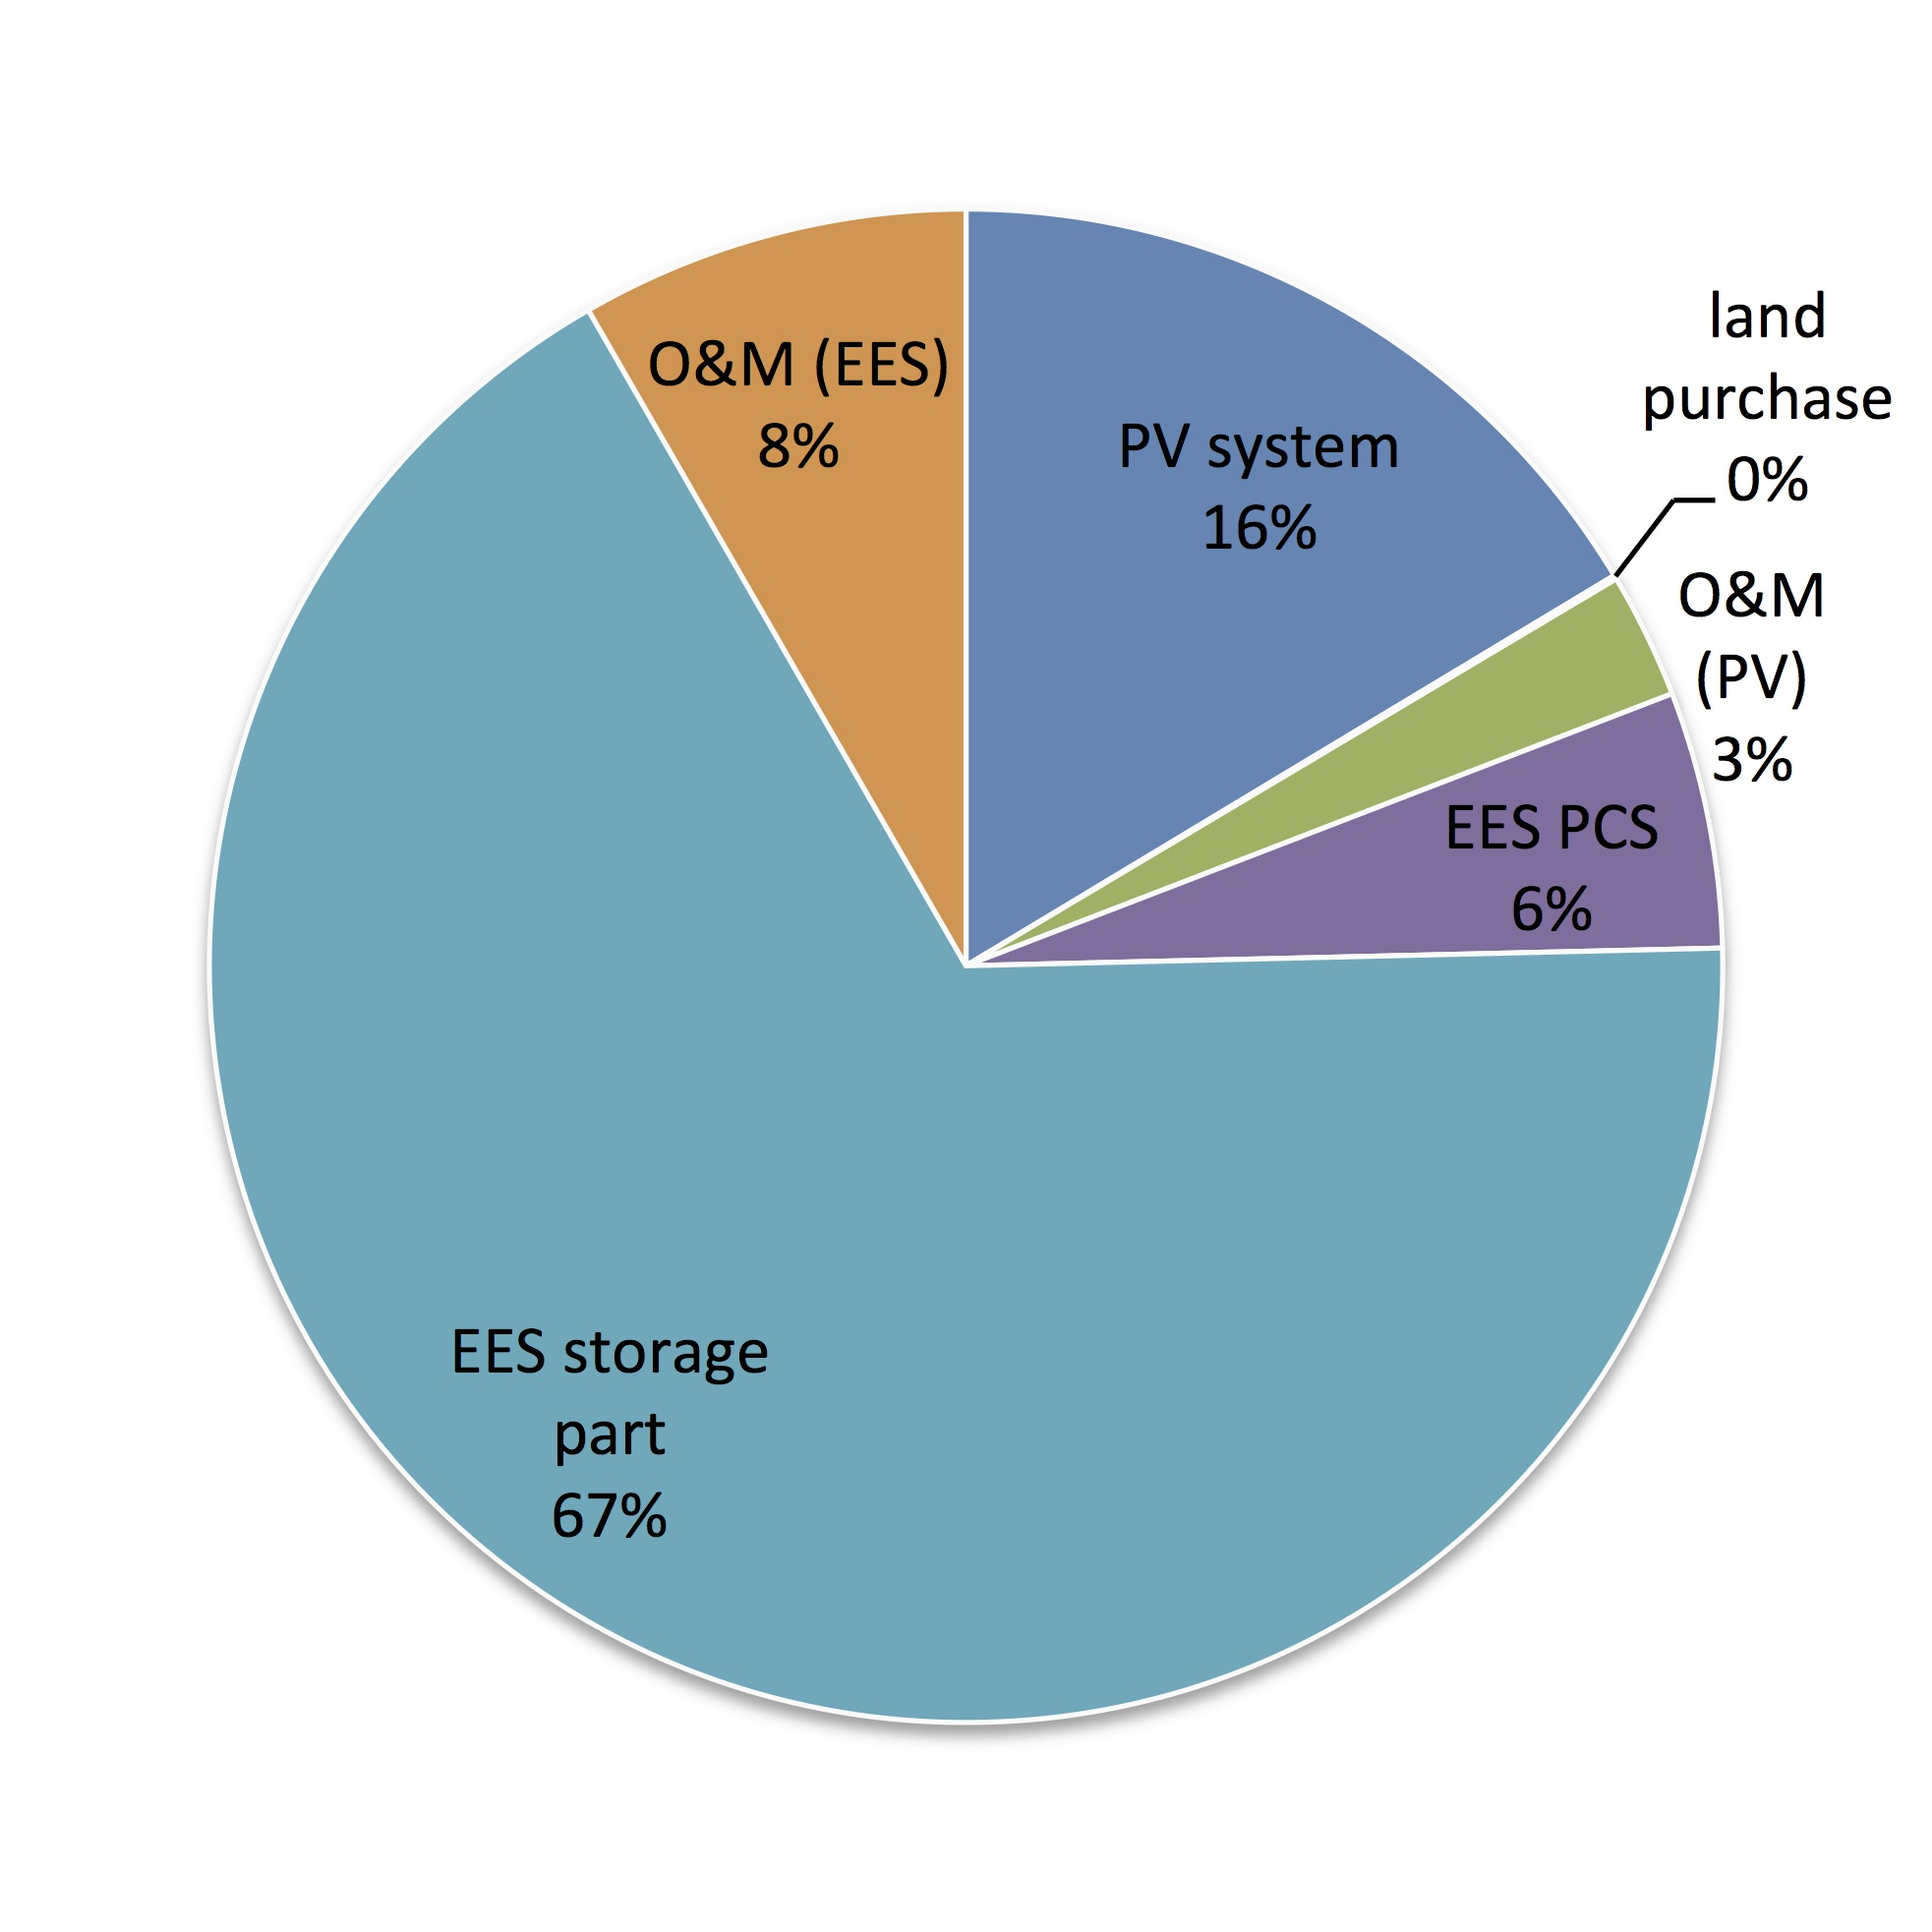
\includegraphics[width=1\textwidth]{FIG/PV_LCOE_lowinvest_BreakDown}
                \caption{LCOE break-down for PVM~2.0 and \SI{4}{h}~EES.}\label{PV_LCOE_lowinvest_BreakDown}
        \end{subfigure}%
        ~
        \begin{subfigure}[b]{0.5\textwidth}
                \centering
                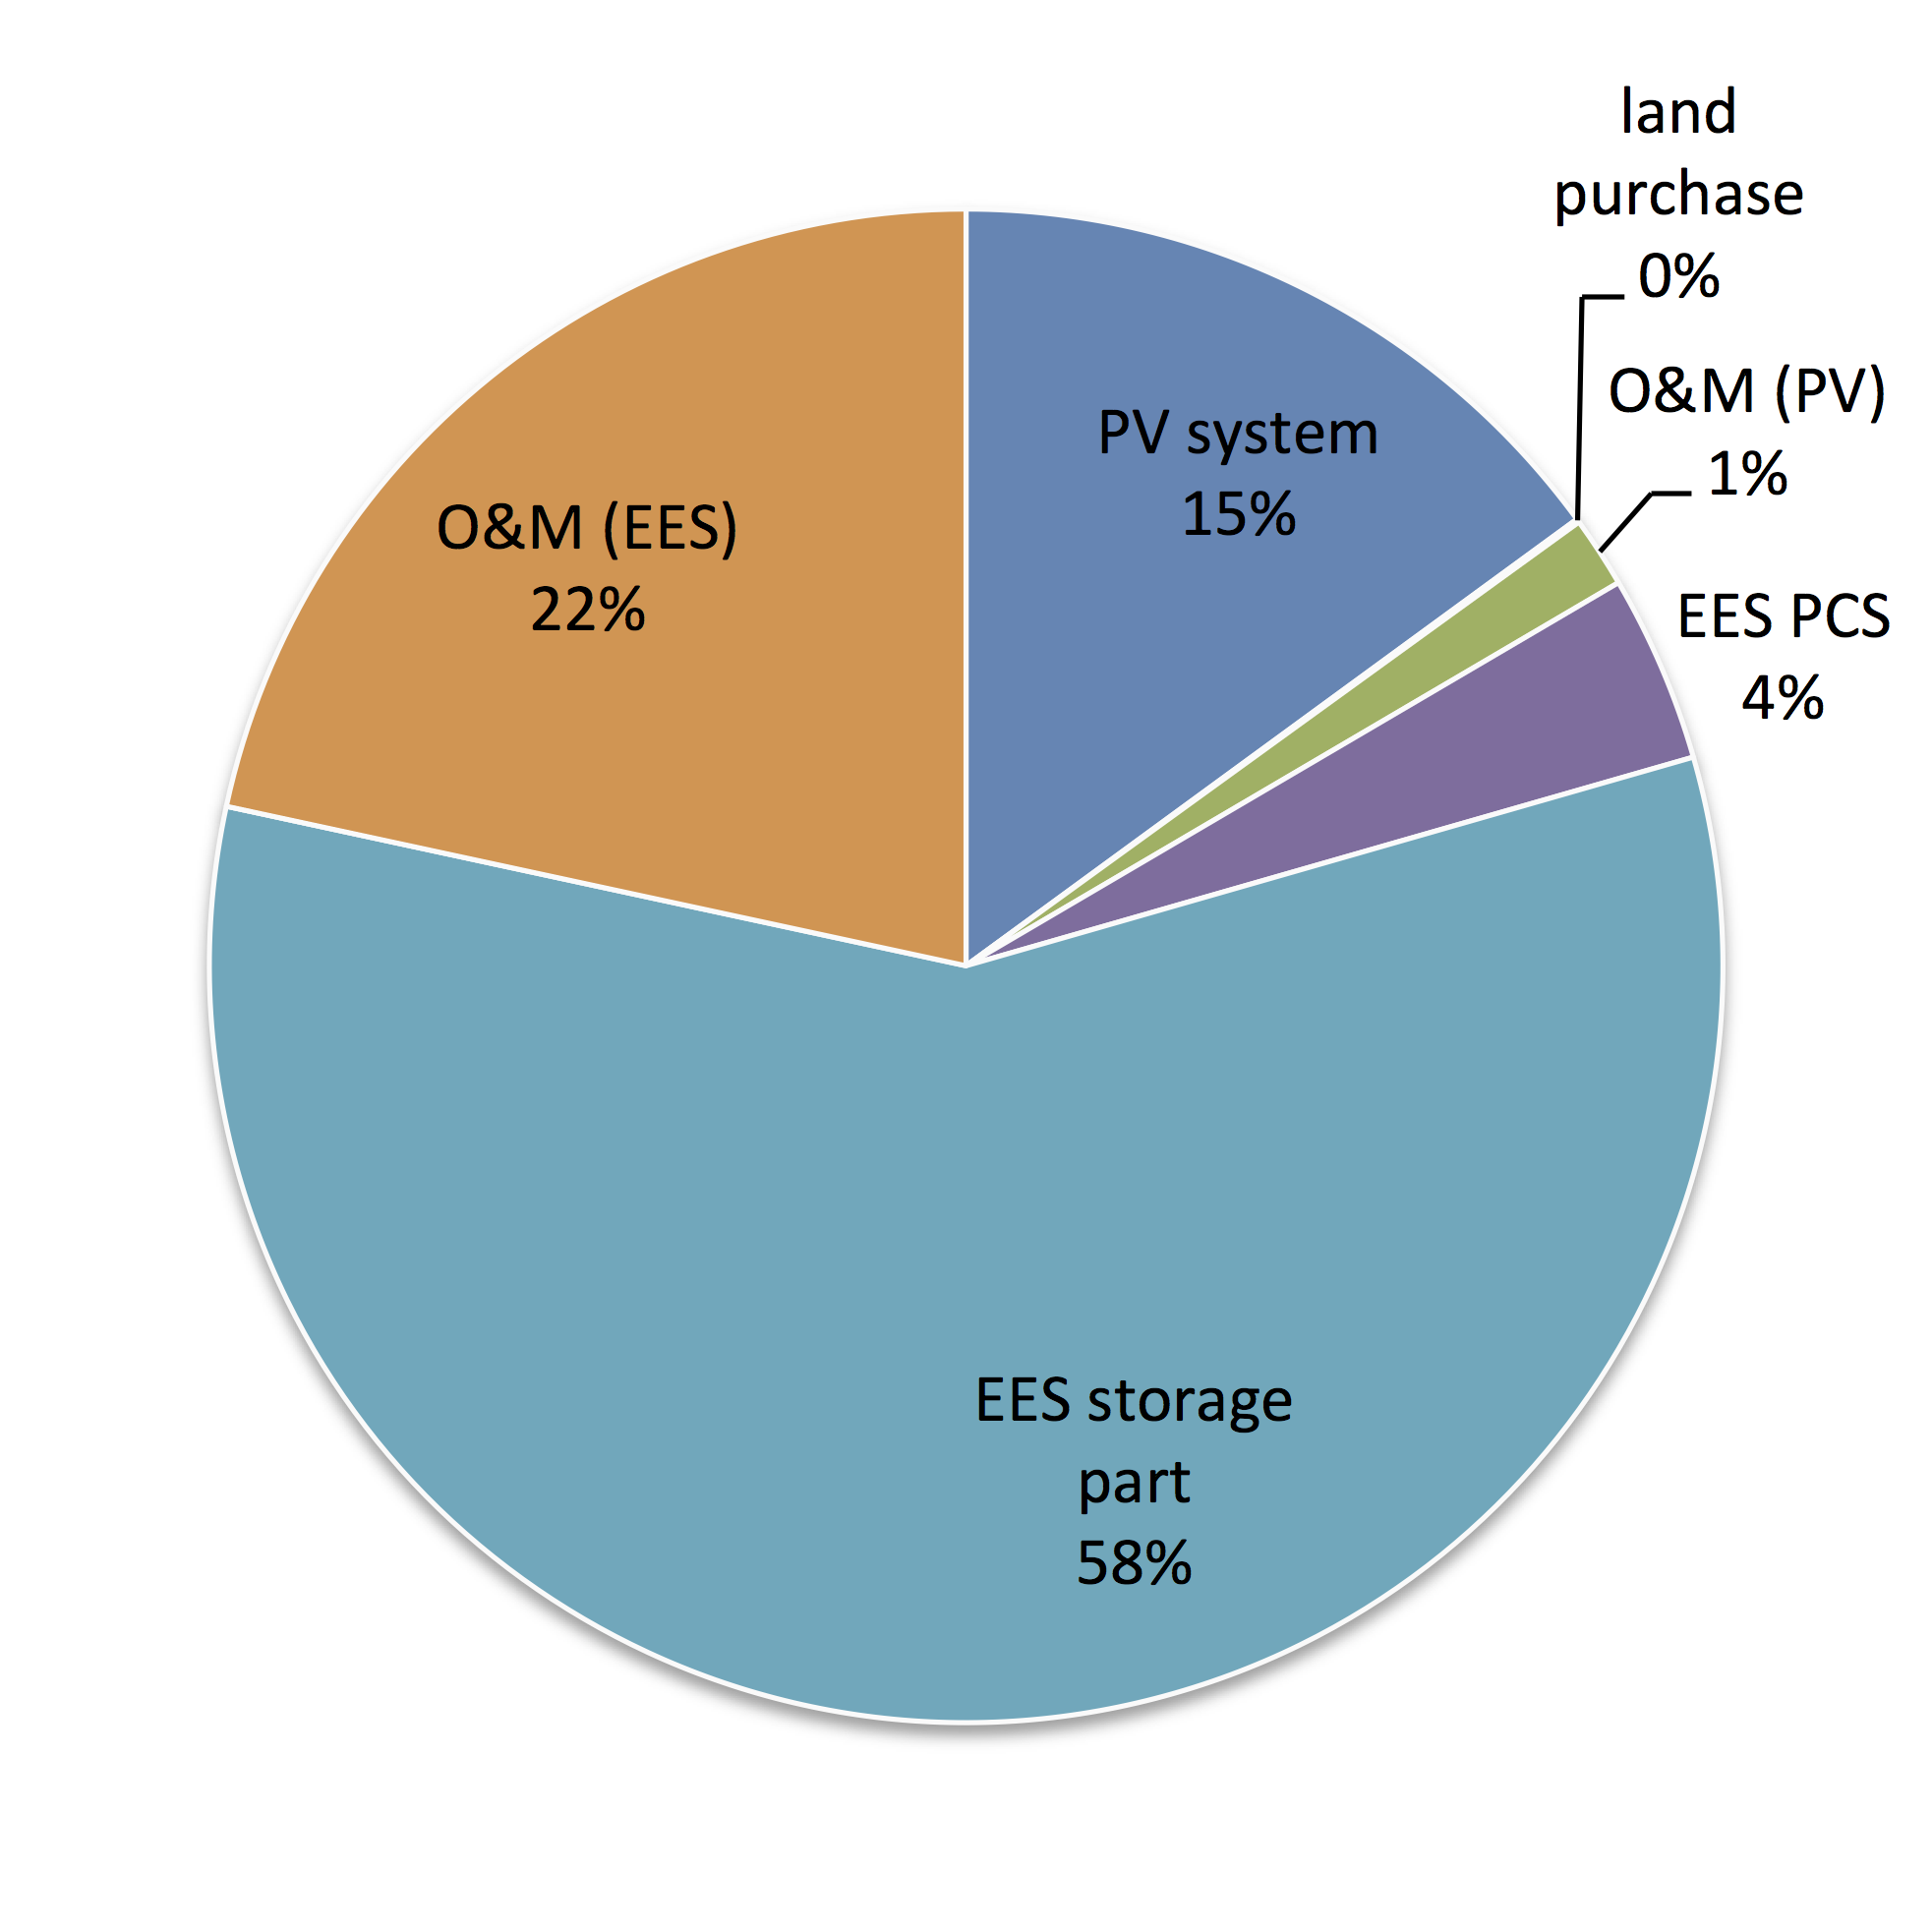
\includegraphics[width=1\textwidth]{FIG/PV_LCOE_highinvest_BreakDown}
                \caption{LCOE break-down for PVM~2.8 and \SI{8}{h}~EES.}\label{PV_LCOE_highinvest_BreakDown}
        \end{subfigure}
        \caption[Break-down of selected LCOE calculation  results of PV systems with adapted EES.]{Break-down of selected LCOE calculation results of PV systems with adapted EES.}\label{SMPV_LCOE_BreakDown}
\end{figure}
Comprising the results of the LCOE calculation and associated load curve covering results shows that for covering 90\% of the predicted load the configuration of PVM 2.8 and \SI{7}{h} of EES reaching the lowest LCOE of \SI{315.39}{USD/MWh}. But the configuration owns an high value of surplus output of about 5.5~\% (see Figure~\ref{PV_energy_output}). The configuration PVM 2.6 reaches also the 90~\% load curve covering with a share of just 2.1~\% surplus output and a LCOE of \SI{322.18}{USD/MWh}.

The lowest LCOE for reaching 80~\% of the prescribed load is \SI{275.18}{USD/MWh} using \SI{5}{h} of EES and also a PVM of 2.6. For reaching 70~\% the 2.2 and \SI{4}{h} of EES reaches the lowest LCOE of \SI{251.83}{USD/MWh}.
\pagebreak
\section{Interpretation and comparison of results}
The previous sections showed that all simulated solar power plants are able to cover the predicted load curve for more than 90~\% over the year using specified configurations. To describe this in a wildly-used indicator, all simulated power plants are reaching a CF of about 73.1~\% in these specified scenario. The selected power plant configuration of each technology to cover the prescribed load at the lowest LCOE are summarized in Table~\ref{tbl: summaryresult}.
\begin{table}[!htbp]  
  \centering
	\begin{tabular}{ p{3.0cm} C{3.6cm} C{3.6cm} C{3.6cm} } 
	\hline	
&\multicolumn{3}{c}{\textbf{Selected configuration to cover the predicted load}}\\

\textbf{Type} & \textbf{$\geq$~70~\%} & \textbf{$\geq$~80~\%} & \textbf{$\geq$~90~\%} \\ \hline \hline
CR power plant 	& SM:~2.0 \& TES:~10~h	& SM:~2.5 \& TES:~10~h & SM:~3.0 \& TES:~14~h \\
PTC power plant	& SM:~3.0 \& TES:~10~h	& SM:~3.5 \& TES:~12~h & SM:~5.0 \& TES:~12~h  \\
PV power plant	& PVM:~2.2 \& EES:~4~h	& PVM:~2.6 \& EES:~5~h & PVM:~2.8 \& EES:~7~h \\
\hline
\end{tabular}
\caption[Summary of selected solar power plant configurations to reach the target load covering at lowest LCOE.]{Summary of selected solar power plant configurations to reach the target load covering at lowest LCOE.}\label{tbl: summaryresult}
\end{table}

The summary in the Table shows, that the expenditure in technical and therefore also in economic terms are quite different between the technologies to reaching higher load curve coverings. When comparing the rising multiple of the design point of the solar power plants to reach a higher amount of annual load covering it seams that the effort is quite different between the technologies. When comparing the necessary growing multiple to the design point of the power plants to reach higher annual load curve covering it seams obviously that the effort of the PTC technology rises at most. The PTC power plant needs a about five-times larger solar field (SM of 5.0) in reference to the design point to cover 90~\% of the predicted load curve. This is particular high, especially in comparison to the SM of the CR power plant system at the same design point which needs just a three times larger heliostat field. As it was shown before in Section~\ref{sec.resultsPTC} the high effort of the PTC technology to reach high load curve covering values is based on the optical efficiency loss of the solar field at low irradiation angle through the cosine effect. The optical efficiency loss through the cosine effect affects also the CR system, but thanks to the two-axis tracking of the heliostats is the influence comparatively small. 

As the solar fields needs to be over scaled to producing enough thermal power for the whole day also in winter times, both CSP technologies needs to reduce the field optical focus fraction in summer times. The average field optical focus fraction, for both CSP technologies from the Table which covers more then 90~\% are shown in Figure~\ref{FocusFraction} for December. Both technology needs to reduce the thermal output of there receivers by optical focus fraction significantly during the December. The December average shows that more than 60~\% of the CR heliostat field is defocused from 13:00 to 15:00 and also the solar field of the PTC plant needs a focus fraction up to over 50~\% in December. 
\begin{figure}[!htbp]
        \centering                
        \begin{subfigure}[b]{0.5\textwidth}
                \centering
                \includegraphics[width=1\textwidth]{FIG/FocusFraction/DecemberCR}
                \caption{Average CR heliostat field focus fraction in December at a SM of 3.0 and 14~h of TES.}\label{DecemberCR}
        \end{subfigure}%
        ~
        \begin{subfigure}[b]{0.5\textwidth}
                \centering
                \includegraphics[width=1\textwidth]{FIG/FocusFraction/DecemberPTC}
                \caption{Average PTC SCA field focus fraction in December at a SM of 5.0 and 12~h of TES.}\label{DecemberPTC}
        \end{subfigure}
        \caption[Average field optical focus fraction in December of for 90~\% load curve covering configurated CSP technologies.]{Average field optical focus fraction in December of for 90~\% load curve covering configurated CSP technologies.}\label{FocusFraction}
\end{figure}

The designed PV power plant is fixed orientated and doesn't track the sun, nevertheless for reaching a covering of 90~\% of the prescribed load over the first year the PV power plant needs a lower multiple of the design point than the other two solar power plants. This mainly comes from the characteristics of the PV system by using GHI instead of DNI. Upington has a huge amount on direct irradiation but also cloudy days with diffuse irradiance (see Figure~\ref{DHI-DIF}). Therefrom the PV power plant needs a lower multiple of the PV system and a smaller storage compared to the CSP power plants. Also the surplus net output of the simulated PV power plants is just about 2.2 and 5.5~\% over the year. Compared with the defocused solar field capacities of the CSP plants this is a very small value.

\begin{figure}[htbp]  
\centering
\includegraphics[width=0.8\linewidth]{FIG/90_annual_profil}
\caption[Annual average load profile of selected PV power plant configurations.]{Annual average load profile of selected PV power plant configurations.}\label{90_annual_profil}
\end{figure}
The annual average load profiles of the in Table~\ref{tbl: summaryresult} specified  power plant configuration over 90~\% load covering are compared in Figure~\ref{90_annual_profil}. It can be seen that they profiles of the three solar power plant are relatively equal. But it is noticeable that the PV plant can fully cover the load from 10:00 to 16:00 over the full year. Compared to are the annual average net energy outputs of the CSP plants just below, but can't cover the load like the PV power plant. This mainly comes from the not exactly configurable turbine power output control, which settings was described in the respective simulation design sections. It can be assumed that under real conditions a steam Rankine power output control is working far more accurate. 

As the line chart shows all simulated solar power plants are having there main leak in supply during the morning hours. But this mainly comes from the weaker power generation during the winter time, where the irradiation amount and angle of sunlight radiation is lower. Basically can be said that all three here shown solar power plant covers the load almost continuously over the year, but during the mentioned time during the winter all solar power plants coming to standstill. This can also be seen in the net power output heat maps of Figure~\ref{Heatmap}. The Figures describes the net power output of the selected simulated solar power plants at any hour of the simulated year. It just shows the net power output which is covering  the prescribed load and no surplus net power. It describes therefore the values of the annual average load profile from the line chart above more in detail. The power reduction during the night time from 22:00 to 7:00 is clearly visible in the heat maps. Also can be seen, that all solar power plants has interruptions in supply on various days in the year which leads from low direct or global irradiation at days of bad weather. 

\begin{figure}[!htbp]
        \centering   
        \begin{subfigure}[b]{1\textwidth}
                \centering
                \includegraphics[width=1\textwidth]{FIG/HeatmapCR}
                \caption{CR with a SM of 3.0 and 14~h of TES.}\label{HeatmapCR}
        \end{subfigure}
        
\par\medskip % Linebreak

        \begin{subfigure}[b]{1\textwidth}
                \centering
                \includegraphics[width=1\textwidth]{FIG/HeatmapPTC}
                \caption{PTC with a SM of 5.0 and 12~h of TES.}\label{HeatmapPTC}
        \end{subfigure}
        
\par\medskip % Linebreak     
           
        \begin{subfigure}[b]{1\textwidth}
                \centering
                \includegraphics[width=1\textwidth]{FIG/HeatmapPV}
                \caption{PV with a PVM of 2.8 and 7~h of EES.}\label{HeatmapPV}
        \end{subfigure}
        \caption[Net power output to predicted load from selected solar power plants shown as heat map over the simulated year.]{Net power output to predicted load from selected solar power plants shown as heat map over the simulated year.}\label{Heatmap}
\end{figure}
At first it is obviously when comparing the heat maps that at the time of winter solstice all power plants coming to standstill in the morning hours. When taking a view at the stating time of the power plants during that time it can be noted that the PV power plant starts about one hour earlier than the other two plants. On one site this leads from the for the PV system usable diffuse share of the GHI at dawn and on the other site from the set power block starting up time of 30 minutes for both CSP plants. It can also be noted, that the PTC system is starting with less power output then the CSP system at these time of the year.

The heat map of the PTC shows a slightly lower power output during the time from 8:00 to 12:00 in summer time. This leads from the above mentioned power output control, but also from high parasitic consumer of the power plant during that time. When taking an eye on the power output of the PV power plant it can be said that the plant fully covers the predicted load over the year from 11:00 to 13:00.

The comparison shows that all solar power plants are able to cover the predicted load with there individual configured systems. But the cost effort is most different between the systems which also reflected in the investment costs and therefrom in the LCOE. Figure~\ref{LCOEcomparision} summarizes the the LCOE calculation results of the solar power plants at different load curve covering from the previous sections and compares them with each other and with public projections. 

It can be seen that the PV system without EES reaches with 51~USD/MWh the lowest LCOE of the simulated power plants, but covers the predicted load curve just about 33~\%. In comparison with other projections can be seen that the PV system in Upington reaches an excellent LCOE. The Fraunhofer ISE institute names the LCOE range for PV systems in 2013 between 80 and 160~USD/GWh (60-120~EUR/GWh using the avarage exchange rate in 2013 of 1.33 USD/EUR \cite{StatistaGmbH2015}) in areas with a GHI from 1~450 to 2~000~kWh/m\textsuperscript{2} \cite{FraunhoferISE2013}. When using the higher GHI value of Upington and the lower assumed invest costs the calculated LCOE seams realistic. The International Energy Agency (IEA) published the LCOE vlaues of the year 2014 in there annual report of "Tracking Clean Energy Progress 2015" \cite{IEA2015}. These values can be assumed for the international average market. But the GHI value of Upington must be noted as above-average.

In order to make the results of the chart more common it might be helpful to remember that a load curve covering (LCC) of 70~\% is equal with a capacity factor of about 57~\% and  a LCC of 90~\% equals a capacity factor of about 73~\% as it was described at the beginning of this Chapter.

When comparing the LCOE results of the simulated solar power plant it must be noted that the degradation of the EES storage is not included in the LCOE calculation of the PV power plant with adapted EES. 

\begin{figure}[htbp]  
\centering
\includegraphics[width=1\linewidth]{FIG/LCOEcomparision}
\caption[Summary of calculated LCOE results of Simulated solar power plants compared with public projections.]{Summary of calculated LCOE results of Simulated solar power plants compared with public projections.}\label{LCOEcomparision}
\end{figure}
The lowest LCOE calculation results of the simulated solar power plants which covers more than 90~\% of the predicted load curve has the CR power plant with about 150~USD/MWh. The CR power plant in generally reaches the lowest LCOE values while having a high load curve covering rate. Also the LCOE result of the PTC power plant is with 189~USD/MWh relatively low. When comparing this values with the projections of Fraunhofer ISE institute and IEA they are looking quite optimistic. 

When taking an eye on the LCOE calculation results of the simulated PV power plant it is obviously that they are much more expansive then the CSP power plants. The LCOE of the cheapest PV power plant which reaches the 90~\% LCC is about twice that high than that from the CR power plant. For the comparison also must be remembered, that the costs of the EES storage part was assumed extremely low in comparison with the average marked price. But when using other optimistic LCOE calculations of battery EES the result seams realistic. Vassallo calculated a LCOE of a battery EES with about 200~USD/MWh pure storage costs \cite{Corcuera2015}. This also goes in hands with the battery EES LCOE results from Zakeri. He names the range of LCOE for battery storage between 278 and 821~USD/MWh (209 -617~EUR/MWh exchange rate 1.33 USD/EUR \cite{StatistaGmbH2015})   at a energy price of 66.5~USD/MWh and 8\% interest rate\cite{Zakeri2015}. However he results the LCOE of the Li-Ion battery at the top end.




\begin{figure}[!htbp]
        \centering                
        \begin{subfigure}[b]{0.5\textwidth}
                \centering
                \includegraphics[width=1\textwidth]{FIG/CR_LCOE_90_BreakDown}
                \caption{LCOE break-down for .}\label{CR_LCOE_90_BreakDown}
        \end{subfigure}%
        ~
        \begin{subfigure}[b]{0.5\textwidth}
                \centering
                \includegraphics[width=1\textwidth]{FIG/PTC_LCOE_90_BreakDown}
                \caption{LCOE break-down for .}\label{PTC_LCOE_90_BreakDown}
        \end{subfigure}
\par\medskip % Linebreak   
        \begin{subfigure}[b]{0.5\textwidth}
                \centering
                \includegraphics[width=1\textwidth]{FIG/PV_LCOE_90_BreakDown}
                \caption{LCOE break-down for .}\label{PV_LCOE_90_BreakDown}
        \end{subfigure}
        \caption[Break-down of selected LCOE calculation results of PV systems with adapted EES.]{Break-down of selected LCOE calculation results of PV systems with adapted EES.}\label{SMPV_LCOE_BreakDown}
\end{figure}


Spinnennetzdiagramm 
PV unity scale without storage 
6-7.5 €cent/kWh (GHI 2000kWh/m2) in 2013 \cite{FraunhoferISE2013}\\\\

